% !TEX program = xelatex
% Free Energy to LLMs｜生成模型与概率统计：从变分自由能到大模型的推理和训练
\documentclass[UTF8,fontset=none,a4paper,11pt,openany]{ctexrep}

\usepackage{geometry}
\geometry{top=24mm,bottom=24mm,left=25mm,right=25mm,headheight=22.2pt}
\usepackage{microtype}
\usepackage{amsmath,amssymb,mathtools,bm}
\usepackage{booktabs,tabularx,array,multirow,longtable}
\usepackage{enumitem}
\usepackage{graphicx}
\usepackage{float}
\usepackage{tikz}
\usetikzlibrary{arrows.meta,positioning,calc,fit,shapes.geometric,shapes.misc,backgrounds,matrix,decorations.pathreplacing,patterns.meta}
\usepackage[most]{tcolorbox}
\usepackage{xcolor}
\usepackage{fancyhdr}
\usepackage{titlesec}
\usepackage{caption}
\usepackage{siunitx}
\usepackage{needspace}
\usepackage{eso-pic}
\usepackage{hyperref}
\usepackage{bookmark}
\usepackage[backend=biber,style=authoryear,sorting=nyt,maxbibnames=3,maxcitenames=2]{biblatex}

% CJK fonts for the book, the figures and the slides.
% Noto Sans CJK SC (SIL Open Font License) is the same typeface as Source Han Sans SC.
% macOS: brew install --cask font-noto-sans-cjk-sc
% Debian/Ubuntu: apt install fonts-noto-cjk
\setCJKmainfont[BoldFont={Noto Sans CJK SC Bold}]{Noto Sans CJK SC}
\setCJKsansfont[BoldFont={Noto Sans CJK SC Bold}]{Noto Sans CJK SC}
\setCJKmonofont{Noto Sans CJK SC}

\graphicspath{{../figures/}}

\definecolor{Navy}{HTML}{14324A}
\definecolor{Teal}{HTML}{0E7490}
\definecolor{Sky}{HTML}{E7F5F8}
\definecolor{Orange}{HTML}{D97706}
\definecolor{Amber}{HTML}{FFF3D6}
\definecolor{Ink}{HTML}{1F2937}
\definecolor{Slate}{HTML}{64748B}
\definecolor{CitationGray}{HTML}{6B7280}
\definecolor{Mist}{HTML}{F5F7FA}
\definecolor{Rose}{HTML}{9F1239}
\definecolor{RoseMist}{HTML}{FFF1F2}

\hypersetup{colorlinks=true,linkcolor=Navy,citecolor=CitationGray,urlcolor=Teal,pdftitle={生成模型与概率统计：从变分自由能到大模型的推理和训练},pdfauthor={张士欣}}
\AtEveryCite{\color{CitationGray}\footnotesize}
\urlstyle{same}
\setlist[itemize]{leftmargin=2em,itemsep=2pt,topsep=3pt}
\setlist[enumerate]{leftmargin=2em,itemsep=3pt,topsep=3pt}
\setlength{\parindent}{2em}
\setlength{\parskip}{0.35em}
\captionsetup{font=small,labelfont={bf,color=Navy},labelsep=space}

\pagestyle{fancy}
\setlength{\headheight}{22.2pt}
\fancyhf{}
\fancyhead[R]{\small\color{Slate}生成模型与概率统计}
\fancyfoot[C]{\small\color{Slate}\thepage}
\renewcommand{\headrulewidth}{0.4pt}
\renewcommand{\headrule}{\hbox to\headwidth{\color{Teal}\leaders\hrule height \headrulewidth\hfill}}

\titleformat{\chapter}[display]{\normalfont\bfseries\color{Navy}}{\filleft\fontsize{42}{46}\selectfont\thechapter}{0.4em}{\filright\Huge}
\titlespacing*{\chapter}{0pt}{-10pt}{24pt}
\titleformat{\section}{\Large\bfseries\color{Navy}}{\thesection}{0.7em}{}
\titleformat{\subsection}{\large\bfseries\color{Teal}}{\thesubsection}{0.6em}{}

\newtcolorbox{keybox}[1][]{enhanced,breakable,colback=Sky,colframe=Teal,boxrule=0.7pt,arc=2mm,left=4mm,right=4mm,top=2mm,bottom=2mm,title={#1},fonttitle=\bfseries\color{Navy}}
\newtcolorbox{warningbox}[1][]{enhanced,breakable,colback=RoseMist,colframe=Rose,boxrule=0.7pt,arc=2mm,left=4mm,right=4mm,top=2mm,bottom=2mm,title={#1},fonttitle=\bfseries\color{Rose}}
\newtcolorbox{examplebox}[1][]{enhanced,breakable,colback=Mist,colframe=Slate,boxrule=0.5pt,arc=2mm,left=4mm,right=4mm,top=2mm,bottom=2mm,title={#1},fonttitle=\bfseries\color{Navy}}

\tikzset{
  flow/.style={-{Latex[length=2.2mm]},line width=0.8pt,color=Slate},
  block/.style={draw=Navy,fill=white,rounded corners=2pt,minimum height=8mm,minimum width=25mm,align=center,font=\small},
  tealblock/.style={block,draw=Teal,fill=Sky},
  orangeblock/.style={block,draw=Orange,fill=Amber},
  softblock/.style={block,draw=Slate,fill=Mist},
  tiny/.style={font=\scriptsize,align=center},
}

\newcommand{\R}{\mathbb{R}}
\newcommand{\E}{\mathbb{E}}
\newcommand{\KL}{\mathrm{KL}}
\newcommand{\softmax}{\operatorname{softmax}}
\newcommand{\diag}{\operatorname{diag}}
\newcommand{\argmin}{\operatorname*{arg\,min}}
\newcommand{\argmax}{\operatorname*{arg\,max}}
\newcommand{\good}[1]{\textcolor{Teal}{#1}}
\newcommand{\note}[1]{\textcolor{Orange}{#1}}

\addbibresource{references.bib}

\begin{document}
\pagecolor{white}
\AddToShipoutPictureBG{\AtPageLowerLeft{\color{white}\rule{\paperwidth}{\paperheight}}}

\begin{titlepage}
\thispagestyle{empty}
\begin{tikzpicture}[remember picture,overlay]
  \fill[white] (current page.south west) rectangle (current page.north east);
  \fill[Navy] (current page.north west) rectangle ([yshift=-8.25cm]current page.north east);
  \fill[Teal] ([yshift=-8.25cm]current page.north west) rectangle ([yshift=-8.60cm]current page.north east);
  \fill[Orange] ([yshift=-8.60cm]current page.north west) rectangle ([yshift=-8.73cm]current page.north east);
\end{tikzpicture}
\vspace*{1.7cm}
{\color{white}\sffamily\small FREE ENERGY TO LLMS\par}
\vspace{1.1cm}
{\color{white}\sffamily\fontsize{31}{38}\selectfont\bfseries 生成模型与概率统计\par}
\vspace{1.35cm}
{\centering\color{Navy}\sffamily\fontsize{16}{22}\selectfont 从变分自由能到大模型的推理和训练\par}
\vspace{2.5cm}
\begin{center}
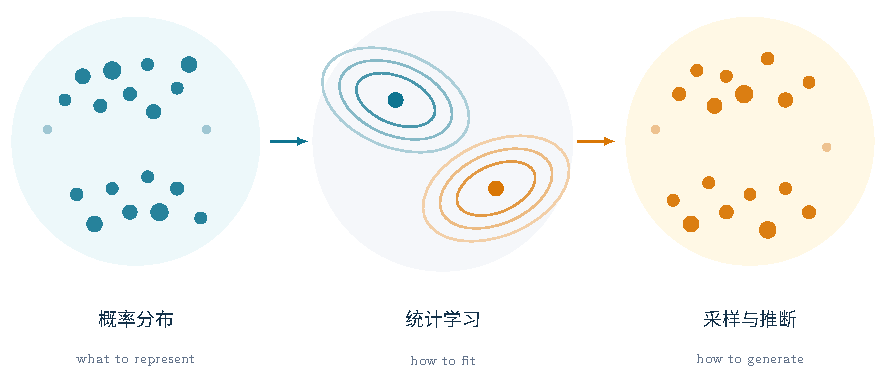
\includegraphics[width=0.96\textwidth]{cover_probability_flow.pdf}
\end{center}
\vfill
\begin{center}
\color{Navy}\sffamily\large 张士欣\par
\vspace{3mm}
\color{Slate}\normalsize 中国科学院物理研究所\quad 2026.10\par
\end{center}
\end{titlepage}


\pagenumbering{roman}
\chapter*{使用说明}
\addcontentsline{toc}{chapter}{使用说明}
本讲义围绕一个问题展开：给定像素、文本单元（token，可以是一个字、子词或符号）、原子坐标、自旋构型或量子态系数等高维对象，如何表达、学习并采样一个合理的概率分布？生成模型在这里指的是一整套方法：把概率建模、统计推断、数值采样和系统实现连接起来，回答同一个对象空间上的分布问题。

\begin{keybox}[本讲义的四个视角]
每个模型都可以从下面四个视角去看，后文讨论任何一个新方法时，都回到这四个问题：
\begin{enumerate}
  \item \textbf{概率对象：}模型表示的是显式密度、条件概率、隐式分布、对数密度梯度还是能量？
  \item \textbf{统计目标：}训练在做最大似然估计、变分下界、对抗匹配、对数密度梯度匹配，还是约束分布变化幅度的奖励优化？
  \item \textbf{计算路径：}采样是一次前向、逐 token 解码、可逆变换、随机微分方程积分，还是马尔可夫链蒙特卡洛？
  \item \textbf{系统瓶颈：}真正限制规模的是浮点运算次数、显存容量、显存带宽、跨卡通信、随机步数，还是数据质量？
\end{enumerate}
\end{keybox}


\tableofcontents
\clearpage
\pagenumbering{arabic}

\chapter{从函数拟合到概率分布}
\label{chap:probability-language}

\begin{keybox}[从拟合函数到拟合分布]
监督学习拟合的是一条从输入到答案的映射；生成模型要拟合的是对象空间上的整个分布。这一章先把这条跳跃拆开：损失函数在优化什么、梯度怎样沿计算图传回、判别与生成分别回答哪个条件概率、以及怎样比较两个分布。KL 的方向和变分自由能会在这里第一次出现，后面判断一个模型是覆盖所有模式还是只抓住一个，都要回到这两个量。
\end{keybox}

\section{一条训练链：从样本到参数更新}

\subsection{分类、拟合与损失函数}

先看最普通的监督学习。数据集 \(\mathcal D=\{(x_i,y_i)\}_{i=1}^N\) 给出输入及其已知答案；例如 \(x_i\) 可以是一个自旋构型，\(y_i\) 是相标签或能量。\textbf{分类}要求预测有限个类别：二分类时 \(y_i\in\{0,1\}\)，模型可输出属于第 1 类的概率 \(q_\theta(x_i)\in(0,1)\)，再用阈值作出类别判断。若答案是连续的能量数值，任务则是回归。两者都先选择一个带可调参数 \(\theta\) 的函数 \(f_\theta(x)\)，再用数据决定参数的取值；这就是函数的\textbf{参数化}与\textbf{拟合}。参数可以是线性模型的系数，也可以是神经网络各层的权重和偏置。

拟合需要把预测好坏化成可计算的标量。逐样本损失 \(\ell\) 衡量预测与答案的差异，经验损失是数据集上的平均：
\begin{equation}
  L(\theta)=\frac{1}{N}\sum_{i=1}^N \ell\bigl(f_\theta(x_i),y_i\bigr).
  \label{eq:basic-empirical-loss}
\end{equation}
对连续目标，常用均方误差（Mean Squared Error，MSE）对应的逐样本平方损失 \(\ell_{\mathrm{MSE}}=(f_\theta(x)-y)^2\)；对二分类概率，常用交叉熵（Cross-Entropy，CE）
\begin{equation}
  \ell_{\mathrm{CE}}=-y\log q_\theta(x)-(1-y)\log\bigl(1-q_\theta(x)\bigr).
  \label{eq:basic-binary-ce}
\end{equation}
预测的正确类别概率越小，交叉熵越大；多分类时相应地在所有类别上输出归一化概率，并取真实类别概率的负对数。损失函数说明\textbf{训练时优化什么}，分类正确率等评价量则说明\textbf{最终怎样衡量表现}，两者可以不同。训练集上的低损失只说明已见样本拟合得好，还需要用未参与参数更新的验证或测试数据检查泛化。

\subsection{梯度下降与自动微分}

当 \(L(\theta)\) 对参数可微时，梯度 \(\nabla_\theta L\) 给出每个参数微小变化对损失的一阶影响。最简单的梯度下降更新为
\begin{equation}
  \theta_{k+1}=\theta_k-\eta\nabla_\theta L(\theta_k),
  \label{eq:basic-gradient-descent}
\end{equation}
其中 \(\eta>0\) 是学习率；实际训练常用随机抽取的一小批样本估计梯度，并使用自适应优化器。优化是反复计算预测、损失和梯度，再更新参数的过程。梯度下降寻找的是当前参数附近的下降方向，不保证在非凸问题中找到全局最优，也不能单独保证泛化。

自动微分把实际执行的计算拆成加法、矩阵乘法、激活函数等基本运算，记录它们构成的计算图，再按链式法则求导。训练神经网络通常使用反向模式：先前向得到损失标量，再从损失沿计算图反向累积 \(\partial L/\partial\theta\)，这就是反向传播。自动微分负责计算梯度，梯度下降或 Adam 等优化器负责利用梯度改变参数；它们是训练链中的两个不同步骤。自动微分沿计算图求得程序中各可微运算的导数；遇到离散抽样等不可直接求导的步骤，还需要另外设计梯度估计方法。

\section{为什么神经网络适合表示函数}

多层感知机（Multilayer Perceptron，MLP）是最基本的前馈神经网络。一个含单个隐藏层的例子是
\begin{equation}
  f_\theta(x)=W_2\,\sigma(W_1x+b_1)+b_2,
  \qquad \theta=(W_1,b_1,W_2,b_2),
  \label{eq:basic-mlp}
\end{equation}
其中矩阵乘法混合输入分量，非线性激活 \(\sigma\) 让模型能表达弯曲的决策边界或非线性响应；若去掉激活，多层仿射变换仍只是一个仿射变换。增加层数就是反复组合这两种操作。用于二分类时，可把标量输出当作 logit，经 sigmoid 函数 \(q_\theta(x)=1/(1+e^{-f_\theta(x)})\) 变成概率；用于回归时，可以直接输出数值。网络的特征变换由数据共同学习，参数可沿计算图求梯度，矩阵运算也适合批量计算。图像、序列等结构化输入通常需要卷积、注意力等进一步的结构设计，后文的 Transformer 就是一种例子。

\textbf{通用近似定理}给出表达能力的一个边界：对紧致区域上的连续函数，在合适的非线性激活条件下，单隐藏层网络只要有足够多的隐藏单元，就能把函数逼近到任意指定的精度~\cite{cybenko1989approximation,hornik1991approximation}。这是一个\textbf{存在性}结论，描述表达能力的上限；实际能否学到还取决于样本量、优化和归纳偏置。神经网络实用的原因还包括可学习的组合特征、可扩展的计算以及对任务结构的适配。接下来把网络输出从数值或类别概率推广到整个数据分布，就进入生成模型的问题。

\section{判别、生成与逆向设计}

判别模型通常直接学习 \(p(y\mid x)\) 或一个决策函数，目标是给定观测 \(x\) 预测标签 \(y\)。生成模型试图刻画 \(p(x)\)，或者在给定条件 \(c\) 后刻画 \(p(x\mid c)\)，从而可以生成新的样本、补全缺失变量、估计似然或做逆向设计（图 \ref{fig:discriminative-generative}）。

\begin{figure}[ht]
\centering
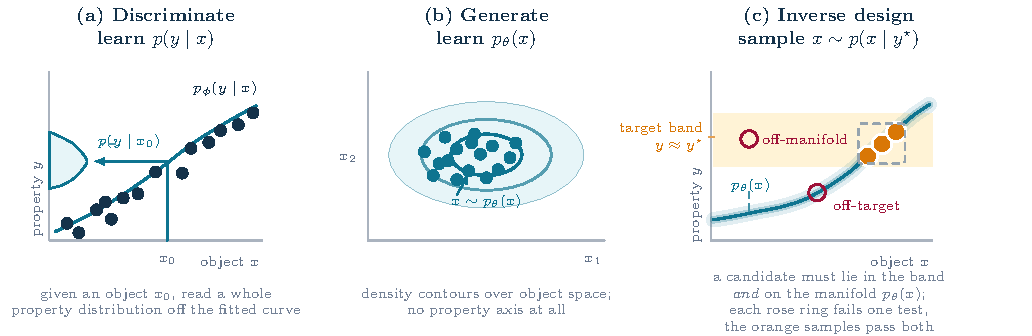
\includegraphics[width=\textwidth]{discriminate_generate_inverse.pdf}
\caption{三个任务使用同一批对象，却回答不同问题：判别模型沿已知对象预测性质；生成模型学习对象空间的概率质量；逆向设计只在目标性质带内寻找仍位于合理数据分布上的候选。}
\label{fig:discriminative-generative}
\end{figure}

贝叶斯公式（Bayes' rule）把这两个方向连接起来：
\begin{equation}
  p(x\mid y)=\frac{p(y\mid x)p(x)}{p(y)}\propto p(y\mid x)p(x).
\end{equation}
这条公式把生成问题中的三个概率对象连接起来，是一段纯粹的恒等变形，不需要任何神经网络参与。设 \(x\) 是待生成的候选结构、分子、图像或文本，\(y\) 是由它产生的观测、类别或目标性质。\(p(x)\) 是先验或无条件生成分布，表示什么样的 \(x\) 在数据中本来就合理；\(p(y\mid x)\) 是正向模型或似然，表示给定候选 \(x\) 后观察到目标 \(y\) 的概率；\(p(x\mid y)\) 是逆向问题真正需要的后验，表示在满足目标 \(y\) 的候选中，哪些 \(x\) 仍然符合数据分布。

例如，设 \(x\) 是候选分子，\(y^\star\) 是目标带隙。训练好的生成模型 \(p_\theta(x)\) 描述哪些分子通常合理，性质预测器 \(p_\phi(y^\star\mid x)\) 描述这些分子满足目标的程度，两者的乘积给出后验的相对权重。如果任务只需要一个候选，可以固定模型参数、对 \(x\) 最大化这个乘积；如果希望保留多个可行结构及其不确定性，就应从后验中采样。仅最大化性质预测器的输出，可能选到训练分布之外的畸形分子；加入先验后，候选还需要得到结构分布的支持。

实现条件生成有两条路线（图 \ref{fig:bayes-generative-models}），区别在于条件分布从哪里来。\textbf{先建模再推断}：分别得到 \(p_\theta(x)\) 与 \(p_\phi(y\mid x)\)，对给定的 \(y\) 用贝叶斯公式构造后验。\textbf{直接学习条件分布}：用配对数据 \((x,y)\) 训练一个条件生成器 \(p_\psi(x\mid y)\)，让同一个网络能够处理不同的 \(y\)。例如，条件自回归模型把 \(y\) 放入每一步生成的条件，条件扩散模型把 \(y\) 送入去噪网络；具体采样过程在第 \ref{chap:model-families} 章展开。

两条路线都必须得到归一化的输出分布，但无需用同一种方式计算归一化因子。先建模再推断时，设 \(\widetilde p_y(x)=p_\theta(x)p_\phi(y\mid x)\)，后验为 \(p(x\mid y)=\widetilde p_y(x)/Z_y\)，其中 \(Z_y=\int\widetilde p_y(x)\,dx\) 通常难算。直接学习条件分布时，归一化由模型构造保证，例如自回归模型的每个条件概率都在词表上归一化，扩散模型由归一化的反向转移逐步采样。这条路线需要足够的配对数据，并承担模型近似和训练误差；它不需要额外计算上述乘积模型的 \(Z_y\)。

回到上面的分子例子，用三个候选把这一步算出来。设它们的先验为 \(p(x_A),p(x_B),p(x_C)=(0.5,0.3,0.2)\)，性质预测器给出 \(p(y^\star\mid x)=(0.1,0.6,0.4)\)。把两项相乘再做归一化，就得到每个候选在后验中的权重（表 \ref{tab:inverse-design-weights}）。

\begin{table}[H]
\centering\small
\begin{tabularx}{\textwidth}{>{\bfseries}p{16mm} X X X X}
\toprule
候选 & 先验 \(p(x)\) & 性质似然 \(p(y^\star\mid x)\) & 乘积 \(\widetilde p_y(x)\) & 归一化后验\\
\midrule
A & 0.5 & 0.1 & 0.05 & 0.16\\
B & 0.3 & 0.6 & 0.18 & 0.58\\
C & 0.2 & 0.4 & 0.08 & 0.26\\
\bottomrule
\end{tabularx}
\caption{三个候选的逆向设计权重。\(Z_{y^\star}=0.05+0.18+0.08=0.31\)。}
\label{tab:inverse-design-weights}
\end{table}

候选 B 的性质最匹配，但先验只有 0.3；候选 A 先验最高，性质却不匹配；C 两项都不突出，后验居中。若只按性质预测器排序，B 仍然第一，但当两个候选的性质分数接近时，先验会改变排序——这正是逆向设计里加入 \(p(x)\) 的作用。

对于已经由 \(\widetilde p_y\) 给出的后验，下面两种方法分别通过采样和优化处理难算的 \(Z_y\)。马尔可夫链蒙特卡洛（Markov Chain Monte Carlo，MCMC）设计转移核 \(K(x'\mid x)\)，使目标后验成为平稳分布，即
\begin{equation}
 p(x'\mid y)=\int K(x'\mid x)p(x\mid y)\,dx.
\end{equation}
接受率可以只依赖 \(\widetilde p_y(x')/\widetilde p_y(x)\)，从而约掉 \(Z_y\)。在链具有遍历性等收敛条件、运行足够久且能跨越不同高概率区域时，样本的经验分布才逼近目标后验；通常丢弃一段初始过渡期（burn-in），并检查样本相关性与跨模式移动。

变分推断（Variational Inference，VI）选择一个归一化、可采样且可求密度的分布族 \(q_\varphi(x)\)，通过优化让它接近后验。这里用 Kullback--Leibler 散度（Kullback--Leibler divergence，KL）衡量两个分布的差异，其定义及在本问题中的展开为
\begin{align}
 \KL(q\Vert p)&=\int q(x)\log\frac{q(x)}{p(x)}\,dx,\\
 \KL(q_\varphi\Vert p(\cdot\mid y))
 &=\E_{q_\varphi}\!\left[\log q_\varphi(x)-\log\widetilde p_y(x)\right]+\log Z_y.
 \label{eq:vi-normalizer}
\end{align}
固定先验、性质预测器和条件 \(y\) 后，\(Z_y\) 与变分参数 \(\varphi\) 无关。因此最小化第一项就能找到同一个最优 \(q_\varphi\)，虽然无法由此报告 KL 的绝对数值。优化完成后，从 \(q_\varphi\) 采样的代价通常较低，误差来自所选分布族和优化结果。若同时改变 \(\theta\) 或 \(\phi\)，\(Z_y\) 一般也会变化，就不能在这些参数的梯度中直接忽略它。

MCMC 与 VI 都可用于“先建模再推断”路线中的后验计算。前者逐步更新样本，后者先拟合近似后验；直接从配对数据训练条件生成器是前面另一层面的建模选择，也可以使用变分训练。这两个层面的选择共同决定需要什么数据、优化什么目标以及最终如何取样。

\begin{figure}[H]
\centering
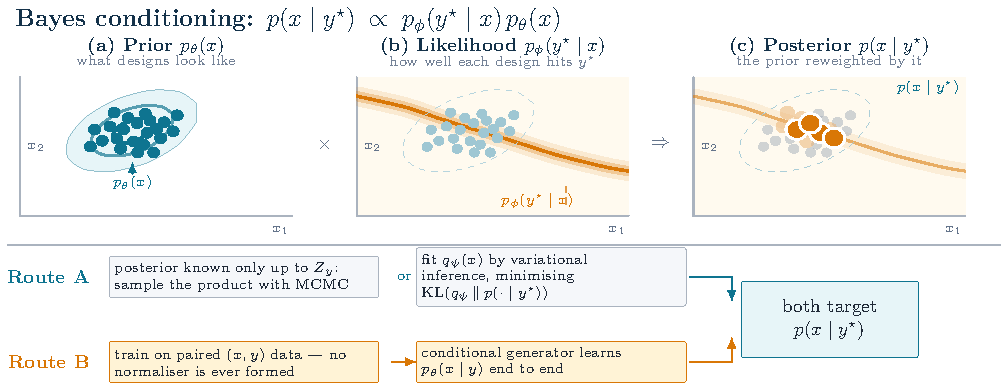
\includegraphics[width=\textwidth]{bayes_conditioning.pdf}
\caption{条件生成的两条建模路线。上方示意先验经目标性质的似然重新加权；路线 A 在给定乘积后验上使用 MCMC 或 VI，路线 B 从配对数据学习条件生成器。两者可以指向同一目标条件分布，有限数据、近似推断和模型误差决定实际差异。}
\label{fig:bayes-generative-models}
\end{figure}

\section{KL 方向与统计物理中的自由能}

\subsection{KL 的方向与模式覆盖}

上一节的 VI 需要选择分布间的差异度量。KL 非负，但带有方向。记 \(p\) 为目标分布（例如数据分布），\(q\) 为模型，则 \(\KL(p\Vert q)\neq\KL(q\Vert p)\)。前者在目标分布上取期望，若某个模式真实出现却被模型赋予极小概率，惩罚会很大，这一方向因此要求模型覆盖数据的全部模式；后者在模型自己的样本上取期望，更关心模型生成的样本是否进入目标分布的高概率区域。同一个散度写在哪一侧，决定了哪些区域的误差被赋予更大权重。

图 \ref{fig:kl-direction} 用单个高斯 \(q\) 拟合等权双峰目标 \(p\)。前向 \(\KL(p\Vert q)\) 在 \(p\) 下取期望，对高斯族的最优解恰好匹配 \(p\) 的均值与方差，于是 \(q\) 横跨两峰，也把质量放进了两峰之间的低谷。反向 \(\KL(q\Vert p)\) 在 \(q\) 下取期望，\(q\) 在 \(p\approx0\) 处的质量受到 \(\log(q/p)\) 的重罚，它只好躲进一个峰，另一个峰被整个丢掉。后文反复回到这两种行为：最大似然训练的模型倾向于覆盖所有模式，样本可能落在模式之间；生成对抗网络（Generative Adversarial Network，GAN）的模式坍缩、后训练中的分布坍缩则更接近反向 KL 的行为。

\begin{figure}[H]
\centering
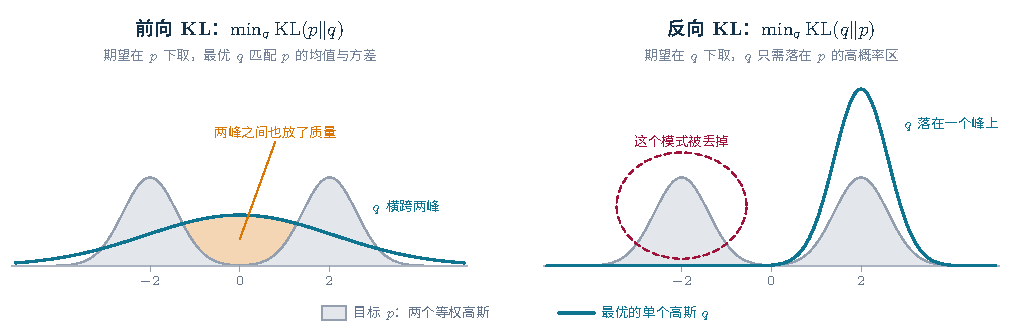
\includegraphics[width=\textwidth]{kl_direction.pdf}
\caption{用单个高斯 \(q\) 拟合双峰目标 \(p\) 时，KL 的两个方向给出不同的最优解。左：前向 \(\KL(p\Vert q)\) 的最优 \(q\) 与 \(p\) 同均值、同方差，覆盖两个模式，同时在两峰之间放了 \(p\) 几乎没有的质量（橙色）。右：反向 \(\KL(q\Vert p)\) 的最优 \(q\) 近似贴合一个峰，丢掉另一个模式；按对称性，落在左峰同样最优。}
\label{fig:kl-direction}
\end{figure}

\subsection{玻尔兹曼分布与变分自由能}
\label{sec:free-energy}

对玻尔兹曼目标 \(\pi(x)=Z^{-1}\exp[-\beta E(x)]\)，任意归一化试探分布 \(q_\theta\) 满足（其中 \(\beta=1/(k_BT)\)，\(T\) 为温度，\(k_B\) 为玻尔兹曼常数）
\begin{align}
 \KL(q_\theta\Vert\pi)&=\E_{q_\theta}[\log q_\theta(x)+\beta E(x)]+\log Z,\\
 F[q_\theta]&=\E_{q_\theta}[E(x)]-T S[q_\theta],\qquad S[q]=-k_B\E_q[\log q].
\end{align}
所以最小化变分自由能等价于最小化 \(\KL(q_\theta\Vert\pi)\)。这条关系将统计物理中的低能量、高熵平衡与生成模型中的样本质量、分布覆盖联系起来。

\begin{figure}[H]
\centering
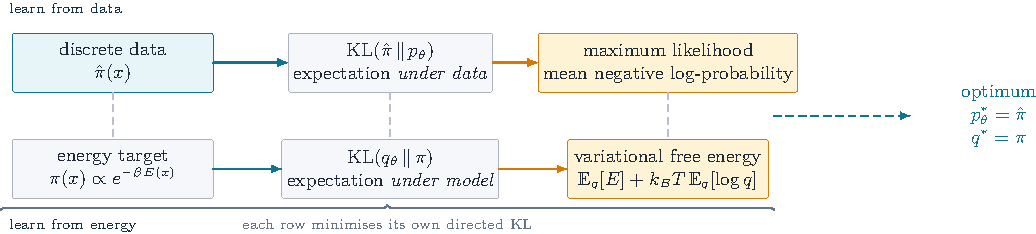
\includegraphics[width=\textwidth]{mle_free_energy.pdf}
\caption{两个方向的 KL 对应不同的学习目标。上行从离散数据学习分布，下行从已知能量学习平衡分布；前者导出下一章的最大似然，后者导出变分自由能。在不限制模型表达能力时，两者各自以匹配其目标分布为最优解。}
\label{fig:mle-free-energy}
\end{figure}

\subsection{从抽样分布看训练梯度}
\label{sec:gradient-estimator-map}

后面几类模型的训练目标都会出现同一步：从一个含参数 \(q_\eta\) 的分布里抽样，再对样本上的目标求期望。先把两条求导路径放在一起，遇到具体模型时可以直接对照；第 \ref{chap:model-families} 章变分自编码器（Variational Autoencoder，VAE）的连续潜变量走重参数化，第 \ref{chap:training-methods} 章的策略梯度走 score-function。

图 \ref{fig:mle-free-energy} 的两行还提示了训练梯度的区别。若样本来自固定的经验分布，且 \(\log p_\theta(x)\) 可以直接求值，最大似然损失满足 \(\nabla_\theta[-\E_{\hat\pi}\log p_\theta(x)]=-\E_{\hat\pi}\nabla_\theta\log p_\theta(x)\)：对每个真实样本直接反向传播即可。若目标包含 \(J(\eta)=\E_{u\sim q_\eta}[h_\eta(u)]\)，而该期望需要从依赖 \(\eta\) 的分布抽样估计，就必须处理参数如何影响被抽到的 \(u\)。两种常用路径是
\begin{align}
 \nabla_\eta J
 &=\E_{q_\eta}\!\left[\nabla_\eta h_\eta(u)
 +(h_\eta(u)-b)\nabla_\eta\log q_\eta(u)\right],
 &&\text{score-function},\\
 \nabla_\eta J
 &=\E_{\epsilon\sim p(\epsilon)}\!\left[
 \frac{d}{d\eta}h_\eta(g_\eta(\epsilon))\right],
 \quad u=g_\eta(\epsilon),
 &&\text{重参数化}.
\end{align}
这里 \(b\) 不依赖当前抽到的 \(u\)，可作为 baseline 降低第一种估计的方差~\cite{zhang2023admc}；第二种写法把随机性移到与 \(\eta\) 无关的 \(\epsilon\)，再沿确定性的 \(g_\eta\) 使用链式法则。两式都保留了 \(h_\eta\) 本身对参数的直接导数。强化学习大量使用第一条路径：策略从 \(\pi_\theta\) 抽取动作或整条轨迹，以回报乘以 \(\nabla_\theta\log\pi_\theta\) 构造蒙特卡洛策略梯度；后文的近端策略优化（Proximal Policy Optimization，PPO）和组相对策略优化（Group Relative Policy Optimization，GRPO）用优势替代原始回报，并加入概率比、裁剪等机制。

\begin{table}[H]
\centering\small
\begin{tabularx}{\textwidth}{>{\bfseries}p{28mm} X X X}
\toprule
梯度路径 & 适用条件 & 梯度从哪里来 & 优势与代价\\
\midrule
Score-function & 可计算并求导 \(\log q_\eta(u)\)；\(u\) 可离散，参数无关的 \(h\) 可为黑盒 & 目标值乘以 \(\nabla_\eta\log q_\eta(u)\) & 适用面广；方差通常较高，常配合 baseline\\
重参数化 & 可写成可微的 \(u=g_\eta(\epsilon)\)，且后续目标对 \(u\) 可微 & 沿 \(h_\eta\) 与 \(g_\eta\) 的计算图回传 & 利用样本方向上的导数，方差通常较低；需要可微路径\\
\bottomrule
\end{tabularx}
\caption{从参数化抽样分布求训练梯度的两条路径。}
\label{tab:gradient-estimator-map}
\end{table}

下文读到新的训练目标时，可先看抽样分布是否含待优化参数，再用表 \ref{tab:gradient-estimator-map} 判断梯度怎样通过采样步骤。VAE 的连续潜变量和 GAN 的连续生成路径使用重参数化一侧的路径梯度；从模型采样离散 token、自旋或线路结构并按评分更新其分布时，常用 score-function。

\chapter{主流生成模型：表达、训练与采样}
\label{chap:model-families}

\begin{keybox}[两条主线：采样与数据概率]
生成模型同时要能采样，也要能计算 \(p_\theta(x)\)：给定分布后取出新样本 \(x\) 是采样，判断一个样本在模型下有多合理是密度。这两件事在同一个模型上很难同时做好。自回归模型两件都容易，代价是采样必须串行；可逆流模型可追踪 \(p_\theta(x)\)，有限层 RealNVP（Real-valued Non-Volume Preserving）与连续归一化流（Continuous Normalizing Flow，CNF）分别付出结构约束和数值积分的成本；对抗生成模型采样极快却根本给不出 \(p_\theta(x)\)；能量模型把 \(p_\theta(x)\) 写成最灵活的形式，代价是采样变成昂贵的马尔可夫链。后续每个模型都沿着这条取舍阅读：先确定它表示什么概率对象；再找到可由数据计算的训练目标；随后把该目标与实际采样算法连接起来；最后定位成本来自串行解码、Jacobian、博弈、积分还是 MCMC 混合。
\end{keybox}

\section{一个统一的比较表}

六类模型的相对位置见图 \ref{fig:model-map}，各自的概率表达与代价见表 \ref{tab:model-families}。自回归模型逐变量生成，变分自编码器先抽取潜变量再解码，可逆流把简单分布连续变形，对抗生成模型通过判别反馈学习，扩散模型逐步去噪，能量模型通过能量高低规定相对概率。连续时间流所用的常微分方程（Ordinary Differential Equation，ODE）在后文推导。GAN 小节后还会讨论另一种只依靠两组样本训练生成器的方法：用核函数计算分布差异，而不训练判别器。

\begin{figure}[H]
\centering
\begin{tikzpicture}[x=1cm,y=1cm,font=\small]
  \draw[Slate!35,dashed] (3.4,0.2) -- (3.4,6.0);
  \draw[Slate!35,dashed] (6.6,0.2) -- (6.6,6.0);
  \draw[Slate!35,dashed] (0.2,2.25) -- (9.7,2.25);
  \draw[Slate!35,dashed] (0.2,4.35) -- (9.7,4.35);
  \draw[->,line width=0.8pt,Slate] (0,0) -- (10.1,0) node[right,font=\small] {似然可算性};
  \draw[->,line width=0.8pt,Slate] (0,0) -- (0,6.5) node[above,font=\small] {采样成本};
  \node[below,font=\scriptsize,text=Slate] at (1.7,0) {精确};
  \node[below,font=\scriptsize,text=Slate] at (5.0,0) {有下界或未归一化};
  \node[below,font=\scriptsize,text=Slate] at (8.3,0) {隐式};
  \node[left,font=\scriptsize,text=Slate,align=right] at (0,1.2) {一次\\前向};
  \node[left,font=\scriptsize,text=Slate,align=right] at (0,3.3) {固定\\$T$ 步};
  \node[left,font=\scriptsize,text=Slate,align=right] at (0,5.4) {迭代到\\混合};
  \node[tealblock,minimum width=25mm] at (1.7,1.2) {Flow\\{\scriptsize 可逆结构}};
  \node[tealblock,minimum width=25mm] at (1.7,3.3) {自回归\\{\scriptsize 串行}};
  \node[softblock,minimum width=25mm] at (5.0,1.2) {VAE\\{\scriptsize 下界}};
  \node[softblock,minimum width=25mm] at (5.0,3.3) {Diffusion\\{\scriptsize $T$ 步}};
  \node[softblock,minimum width=25mm] at (5.0,5.4) {EBM\\{\scriptsize MCMC}};
  \node[orangeblock,minimum width=25mm] at (8.3,1.2) {GAN\\{\scriptsize 无似然}};
\end{tikzpicture}
\caption{六类模型在似然可算性与采样成本上的位置。左下角“精确似然 + 一次采样”只有 Flow 能到，代价是可逆结构限制了表达力；其余模型至少放弃一项。GFlowNet 落在“未归一化”一列，采样是逐步构造，介于 Diffusion 与 EBM 之间。}
\label{fig:model-map}
\end{figure}

\begin{table}[ht]
\centering\small
\begin{tabularx}{\textwidth}{>{\bfseries}p{24mm} X X X}
\toprule
模型家族 & 概率表达 & 训练目标 & 采样与主要代价\\
\midrule
自回归 & $\prod_t p(x_t\mid x_{<t})$ & 最大似然 / 交叉熵 & 逐变量生成，质量稳定但串行延迟高\\
变分自编码器 & $\int p_\theta(x\mid z)p(z)\,dz$ & 变分下界 / 重参数化 & 从 $z$ 得观测分布并采样，潜变量可能被忽略\\
可逆流 & $z=f_\theta(x)$，可逆 & 负对数似然或速度回归 & 逆向运行有限层或积分 ODE\\
对抗生成 & 隐式推送分布 & 对抗博弈 & 一次生成，模式覆盖与稳定性困难\\
Diffusion/\allowbreak Score & 噪声过程的反演 & 去噪、类别预测或 score 回归 & 连续或离散状态下逐步恢复\\
能量模型 & $p(x)\propto e^{-E_\theta(x)}$ & 对比或变分自由能 & MCMC / Langevin，归一化和混合是难点\\
\bottomrule
\end{tabularx}
\caption{生成模型家族的同一组比较问题。}
\label{tab:model-families}
\end{table}

\section{自回归模型：概率分解就是采样程序}
\label{sec:autoregressive}

\subsection{联合概率的链式分解与网络实现}

一句话、一串自旋或一段离散轨迹都可以按顺序写成多个变量。若直接为所有完整序列分配概率，可能的组合会随长度迅速增加；自回归模型改为每次预测一个变量，把复杂的联合分布拆成一组可归一化的条件分布。这里的顺序规定了采样次序，条件分布则需要由具体网络给出。早期神经概率语言模型已经用有限词窗口和神经网络表示下一词的条件概率~\cite{bengio2003neural}。

对序列 \(x=(x_1,\ldots,x_T)\)，链式法则给出
\begin{equation}
 p_\theta(x)=\prod_{t=1}^{T}p_\theta(x_t\mid x_{<t}),\qquad
 \log p_\theta(x)=\sum_{t=1}^{T}\log p_\theta(x_t\mid x_{<t}).
\end{equation}

\Needspace{8\baselineskip}
一个直观的网络实现是 MADE（Masked Autoencoder for Distribution Estimation，掩码自编码密度估计器）~\cite{germain2015made}。它在前馈网络的连接上施加二值掩码，使第 \(t\) 个输出只能依赖 \(x_{<t}\)，不能读取 \(x_t\) 或后面的变量。以二值序列为例，网络输出 \(T\) 个参数，分别给出 \(p_\theta(x_t=1\mid x_{<t})\)；训练时一次前向就能计算所有位置的条件概率，生成时仍须按顺序采样并填入变量。MADE 展示了如何把链式分解落实为网络连接约束。第三章将重点讨论当前大语言模型的主流自回归实现：通过右移输入与因果注意力满足相同依赖约束的 decoder-only Transformer。

\subsection{从经验分布到逐位置训练损失}

为了让真实序列获得较高概率，训练时采用最大似然估计（Maximum Likelihood Estimation，MLE）。设数据集为 \(\mathcal D=\{x^{(i)}\}_{i=1}^N\)，经验分布 \(\hat\pi\) 给每个样本权重 \(1/N\)。对离散数据，
\begin{align}
 \KL(\hat\pi\Vert p_\theta)
 &=\E_{\hat\pi}[\log\hat\pi(x)]-\E_{\hat\pi}[\log p_\theta(x)]\\
 &=\text{与参数无关的常数}-\E_{\hat\pi}[\log p_\theta(x)].
\end{align}
所以最小化这个方向的 KL，等价于最大化训练数据的平均对数似然；实现上使用负对数似然（Negative Log-Likelihood，NLL）作为损失。连续数据的点质量经验分布与连续模型密度之间的 KL 一般为无穷大，此时应直接把样本平均负对数密度作为目标，或先规定数据离散化，不能把上式当作有限 KL 的恒等式。

把上式中的期望写开就得到训练时真正使用的求和形式。经验分布给每个训练样本权重 \(1/N\)，期望于是变成对 \(N\) 个样本取平均，
\begin{equation}
 -\E_{x\sim\hat\pi}\log p_\theta(x)
 =-\frac{1}{N}\sum_{i=1}^{N}\log p_\theta(x^{(i)}).
\end{equation}
如果 \(x^{(i)}=(x^{(i)}_1,\ldots,x^{(i)}_{T_i})\) 是长度为 \(T_i\) 的 token 序列，自回归模型把一个序列的概率分解为
\begin{equation}
 p_\theta(x^{(i)})=\prod_{t=1}^{T_i}p_\theta\!\left(x^{(i)}_t\mid x^{(i)}_{<t}\right),
\end{equation}
于是
\begin{equation}
 -\log p_\theta(x^{(i)})
 =-\sum_{t=1}^{T_i}\log p_\theta\!\left(x^{(i)}_t\mid x^{(i)}_{<t}\right).
\end{equation}
模型在每个真实前缀 \(x^{(i)}_{<t}\) 上输出整个词表 \(\mathcal V\) 上的 softmax 概率向量 \(\pi_{\theta,t}(\cdot\mid x^{(i)}_{<t})\)，训练标签只是其中真实下一个 token 的 one-hot 向量（真实类别处为 1，其余位置为 0） \(e_{x^{(i)}_t}\)。因此单个位置的 CE 为
\begin{equation}
 \operatorname{CE}_{i,t}
 =-\sum_{v\in\mathcal V}e_{x^{(i)}_t}(v)
 \log \pi_{\theta,t}\!\left(v\mid x^{(i)}_{<t}\right)
 =-\log p_\theta\!\left(x^{(i)}_t\mid x^{(i)}_{<t}\right).
\end{equation}
把上一步与最初的 KL 表达式合起来看：每个位置只保留真实 token 那一项的 log 概率，对这些位置求和，恰好就是最小化 \(\KL(\hat\pi\Vert p_\theta)\) 时被丢掉常数项之后剩下的那一块。也就是说，训练时常用的 softmax 交叉熵损失，正是从最大似然目标逐项推出来的。下面比较训练时使用真实前缀与生成时使用模型前缀的计算差别。

\subsection{训练与生成的前缀从哪里来}

同一个概率分解，在训练和生成时对应两种不同的计算组织。下面分别说明这两个术语所指的前缀来源，以及它们如何决定计算量。例子中使用序列开始标记（Beginning of Sequence，BOS）和序列结束标记（End of Sequence，EOS）。例如输入序列从 \(\langle\mathrm{BOS}\rangle,\text{猫},\text{坐},\text{在},\text{垫子}\) 开始。

\textbf{Teacher forcing} 指训练第 \(t\) 个位置时，把数据集中的真实前缀 \(x_{<t}\) 直接喂给模型，要求模型预测真实的下一个 token \(x_t\)。例如四个训练位置分别使用
\begin{equation}
\langle\mathrm{BOS}\rangle\to\text{猫},\quad
\langle\mathrm{BOS}\rangle\text{猫}\to\text{坐},\quad
\langle\mathrm{BOS}\rangle\text{猫}\text{坐}\to\text{在},\quad
\langle\mathrm{BOS}\rangle\text{猫}\text{坐}\text{在}\to\text{垫子}.
\end{equation}
因果 mask 使第 \(t\) 个输出看不到未来 token，所以这四个条件分布可以在一次矩阵前向中并行计算；每个位置都与真实标签比较，损失是它们的交叉熵之和。Teacher forcing 的“forcing”指的是训练时强制使用正确历史，让每个位置都获得稳定的监督信号；概率分解本身在任何时候都保持同一个形式。

\textbf{Ancestral sampling} 可译为按祖先条件逐步采样。“祖先”指链式法则中已经生成的前缀变量：先从
\begin{equation}
x_1\sim p_\theta(\,\cdot\mid\langle\mathrm{BOS}\rangle),
\end{equation}
抽取第一个 token，再把实际抽到的 \(x_1\) 放回条件中，抽取
\begin{equation}
x_2\sim p_\theta(\,\cdot\mid\langle\mathrm{BOS}\rangle,x_1),
\end{equation}
依此得到 \(x_3,x_4,\ldots\)，直到采到 EOS。每一步都可以直接按模型给出的条件分布抽取，也可以先修改这个分布（温度、截断、惩罚等）再抽取；具体做法和它们对分布的影响在第 \ref{sec:decoding} 章展开。采样必须等待前一个 token，因此训练的“并行计算所有位置”和生成的“串行推进前缀”是两个不同的计算过程。

两者的差异会造成 exposure bias：模型训练时总能看到真实前缀，部署时却会看到自己生成的前缀；一旦早期 token 出错，后续条件分布也随之改变。这个差异解释了为什么训练交叉熵很低时，仍需单独检验长序列采样稳定性。

\begin{figure}[H]
\centering
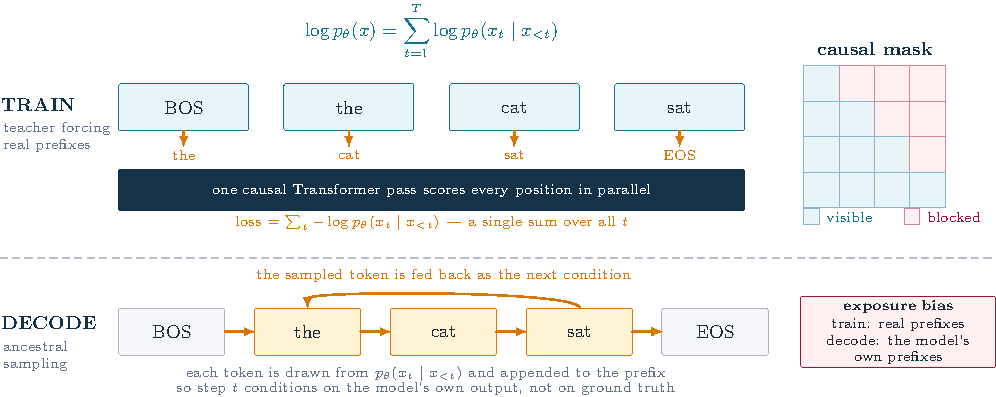
\includegraphics[width=\textwidth]{autoregressive_train_decode.pdf}
\caption{同一个自回归分解有两种计算组织。训练用真实前缀和因果 mask，在一次矩阵前向中并行监督所有位置；生成把刚采到的 token 追加到前缀，因而必须串行推进。}
\label{fig:autoregressive}
\end{figure}

\section{变分自编码器：潜变量与后验推断}

\subsection{潜变量模型与编码、解码}

图像中的姿态、风格或物理构型中的集体坐标，往往比原始数据更低维。VAE 先假设潜变量 \(z\) 的先验，以及给定 \(z\) 后观测 \(x\) 的条件分布；已有 \(x\) 时，再考虑如何推断未被观测的 \(z\)。常说的 encoder 和 decoder 是这两个概率计算方向的神经网络实现名称，出发点仍是潜变量模型与后验推断。

VAE 先假定数据 \(x\) 是由一个低维潜变量 \(z\) 生成的；其核心是把不可直接计算的后验推断改写成可优化的变分下界~\cite{kingma2013vae,rezende2014stochastic}。最常用的模型写成
\begin{equation}
 p_\theta(x,z)=p(z)p_\theta(x\mid z),\qquad
 p_\theta(x)=\int p(z)p_\theta(x\mid z)\,dz,
\end{equation}
其中 \(p(z)=\mathcal N(0,I)\) 是容易采样的先验，\(p_\theta(x\mid z)\) 是观测的条件分布。称作 decoder 的神经网络接收具体的 \(z\)，输出该分布的参数 \(\eta_\theta(z)\)。生成新数据依次需要采样 \(z\sim p(z)\)、计算 \(\eta_\theta(z)\)、再采样 \(x\sim p_\theta(\cdot\mid z)\)；困难在于训练时的边缘似然要对所有可能的 \(z\) 积分。

\subsection{变分下界与重构目标}

如果 decoder 是非线性神经网络，这个积分通常没有解析解，直接最大化 \(\log p_\theta(x)\) 也不能直接得到可反向传播的有限计算图。VAE 引入 encoder \(q_\phi(z\mid x)\) 作为真实后验 \(p_\theta(z\mid x)\) 的可计算近似。常见实现用一个共享的 encoder 主干和两个输出头产生 \(\mu_\phi(x)\) 与 \(\log\sigma_\phi^2(x)\)，定义 \(q_\phi(z\mid x)=\mathcal N\!\left(\mu_\phi(x),\operatorname{diag}\sigma_\phi^2(x)\right)\)。这个高斯分布描述的是给定 \(x\) 后潜变量 \(z\) 的近似后验；decoder 的观测分布 \(p_\theta(x\mid z)\) 则按数据类型选择。训练使用证据下界（Evidence Lower Bound，ELBO），“证据”指观测数据的边缘概率：
\begin{equation}
\begin{aligned}
 \mathcal L_{\mathrm{ELBO}}(x)
 &=\E_{q_\phi(z\mid x)}[\log p_\theta(x,z)-\log q_\phi(z\mid x)]\\
 &=\E_{q_\phi(z\mid x)}[\log p_\theta(x\mid z)]-\KL(q_\phi(z\mid x)\Vert p(z)).
\end{aligned}
\end{equation}
\Needspace{6\baselineskip}
这个目标为何是 \(\log p_\theta(x)\) 的下界？固定模型参数 \(\theta\) 和观测 \(x\)，把 Bayes 公式 \(p_\theta(z\mid x)=p_\theta(x,z)/p_\theta(x)\) 代入并整理，得到
\begin{equation}
\begin{aligned}
 \log p_\theta(x)-\mathcal L_{\mathrm{ELBO}}(x)
 &=\E_{q_\phi(z\mid x)}[\log q_\phi(z\mid x)-\log p_\theta(z\mid x)]\\
 &=\KL(q_\phi(z\mid x)\Vert p_\theta(z\mid x))\geq0.
\end{aligned}
\end{equation}
后验 KL 非负，所以 ELBO 不超过真实对数似然；当 \(q_\phi(z\mid x)=p_\theta(z\mid x)\) 时，两者相等。这个衡量下界松紧的后验 KL，与 ELBO 内部约束 \(q_\phi(z\mid x)\) 接近先验 \(p(z)\) 的 KL 是两个不同的量。真实后验通常也难以逐点计算，因此训练时优化可计算的 ELBO。最大化 ELBO 同时提高 decoder 条件分布对观测 \(x\) 的对数似然，并让 encoder 给出的潜变量分布接近可采样的先验。

第一项 \(\E_q[\log p_\theta(x\mid z)]\) 常叫重构项，实际计算的是已观测到的 \(x\) 在 decoder 所给条件分布下的对数概率。把网络输出的 \(\eta_\theta(z)\) 可视化时，通常得到一幅概率图或均值图；实际样本需另从分布抽取。这一项的具体形式由观测分布决定；选用 Bernoulli 或固定方差高斯分布时，会分别得到交叉熵或均方误差。对于二值数据 \(x\in\{0,1\}^D\)，经典例子让 decoder 输出每一位取 \(1\) 的概率 \(\pi_{\theta,j}(z)\)，并采用给定 \(z\) 后逐位独立的 Bernoulli 观测分布：
\begin{equation}
 p_\theta(x\mid z)=\prod_{j=1}^{D}\pi_{\theta,j}(z)^{x_j}\bigl[1-\pi_{\theta,j}(z)\bigr]^{1-x_j}.
\end{equation}
此时 \(-\log p_\theta(x\mid z)\) 正是逐位 binary cross-entropy；逐位独立只针对给定 \(z\) 的条件分布，边缘分布 \(p_\theta(x)\) 仍可有位与位之间的相关性。对于连续数据，另一种选择是高斯 decoder \(p_\theta(x\mid z)=\mathcal N(\mu_\theta(z),\sigma_x^2I)\)：固定方差时，负重构对数似然等于常数加 \(\|x-\mu_\theta(z)\|^2/(2\sigma_x^2)\)。第二项是 rate 或正则项，要求每个样本的编码分布不要随意偏离 \(p(z)\)，否则从先验采样出来的潜变量无法覆盖训练时的编码区域。

\subsection{重参数化与实际训练}

训练一个 minibatch 时，encoder 输出 \(\mu_\phi(x)\) 和 \(\log\sigma_\phi^2(x)\)，使用
\begin{equation}
 z=\mu_\phi(x)+\sigma_\phi(x)\odot\epsilon,\qquad
 \epsilon\sim\mathcal N(0,I),
\end{equation}
生成一个或少数几个 Monte Carlo 潜变量样本，再送入 decoder。对一个固定的训练样本 \(x\)，用 \(K\) 个独立潜变量样本估计负 ELBO：
\begin{equation}
\begin{aligned}
 \widehat{\mathcal J}_{\mathrm{VAE}}(x)
 &=-\frac{1}{K}\sum_{k=1}^{K}\log p_\theta(x\mid z^{(k)})
 +\KL(q_\phi(z\mid x)\Vert p(z)),\\
 &\hspace{9mm}z^{(k)}\sim q_\phi(\cdot\mid x).
\end{aligned}
\label{eq:vae-mc-loss}
\end{equation}
数据集的损失再对观测 \(x^{(i)}\) 取平均，实践中常取 \(K=1\)。这里每次都用同一个观测 \(x\) 评价 \(\log p_\theta(x\mid z^{(k)})\)，训练重构项时不需要从 decoder 再抽一个 \(x\)。若 \(q_\phi(z\mid x)\) 是对角高斯，KL 项可以精确计算：
\begin{equation}
 \KL\!\left(\mathcal N(\mu,\operatorname{diag}\sigma^2)\Vert\mathcal N(0,I)\right)
 =\frac12\sum_j\left(\mu_j^2+\sigma_j^2-\log\sigma_j^2-1\right).
\end{equation}
这里需要更新的是抽样分布 \(q_\phi(z\mid x)\) 的参数 \(\phi\)，因此使用第 \ref{sec:gradient-estimator-map} 节的重参数化路径。它把随机变量改写为与 \(\phi\) 无关的 \(\epsilon\)，随机性本身保留在 \(\epsilon\) 中，而 \(z\) 对 \(\mu_\phi,\sigma_\phi\) 变成可微的；梯度可以沿 \(x\to(\mu,\sigma)\to z\to\) decoder 反向传播。重构项对 decoder 参数 \(\theta\) 的梯度则是在抽到的 \(z\) 上直接求 \(\nabla_\theta\log p_\theta(x\mid z)\)。图 \ref{fig:vae-network} 把这一步训练画成网络：\(x\) 经 encoder 得到 \(\mu_\phi(x)\) 与 \(\sigma_\phi(x)\)，加入 \(\epsilon\) 抽出 \(z\)，decoder 再把 \(z\) 变回与 \(x\) 同形的 \(\hat x\)；\(\hat x\) 与 \(x\) 比较给出重构损失，\(\mu_\phi,\sigma_\phi\) 与先验比较给出 KL 损失。

\begin{figure}[H]
\centering
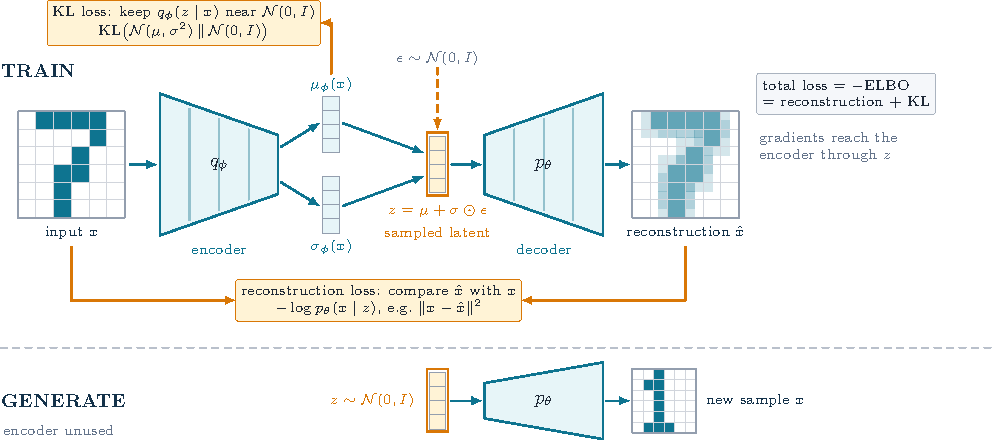
\includegraphics[width=\textwidth]{vae_network.pdf}
\caption{VAE 的网络结构。训练时，encoder 把输入 \(x\) 压缩为 \(q_\phi(z\mid x)\) 的参数 \(\mu_\phi(x),\sigma_\phi(x)\)，由 \(z=\mu+\sigma\odot\epsilon\) 抽出潜变量，decoder 把 \(z\) 展开为重构 \(\hat x\)，即 \(p_\theta(x\mid z)\) 的均值或概率图。重构损失 \(-\log p_\theta(x\mid z)\) 比较 \(\hat x\) 与 \(x\)，KL 损失约束编码分布接近 \(\mathcal N(0,I)\)，两者之和为负 ELBO。生成时不用 encoder，从先验抽 \(z\) 后只运行 decoder。各量之间的概率关系见图 \ref{fig:vae-architecture}。}
\label{fig:vae-network}
\end{figure}

\subsection{生成、重构与后验坍塌}

VAE 的推理有两种含义。生成新样本时从 \(p(z)\) 采样，运行 decoder 得到 \(p_\theta(x\mid z)\) 的参数，再从中采样 \(x\)；分析已有 \(x\) 时运行 encoder 得到 \(q_\phi(z\mid x)\)，可从中采样 \(z\)，再查看 decoder 给出的观测分布。所谓“重构图”通常显示该分布的均值或概率；随机样本需另从该分布抽取。训练复杂度主要是一次 encoder、一次 decoder 和少量潜变量样本，通常不随数据维度做高维积分；建模困难则来自 ELBO 松弛、先验与真实聚合后验不匹配，以及强 decoder 可能不使用潜变量。当 \(q_\phi(z\mid x)\approx p(z)\) 且每个潜变量维度的 KL 接近零时，就出现 posterior collapse；这时观测似然可能仍然很好，但 \(z\) 已经不携带样本特有信息。可以在训练初期减弱 KL 惩罚、随后逐步恢复，让编码器先学会携带样本信息；也可以限制解码器能力，降低其绕过潜变量解释数据的倾向~\cite{bowman2016generating}。

\begin{figure}[H]
\centering
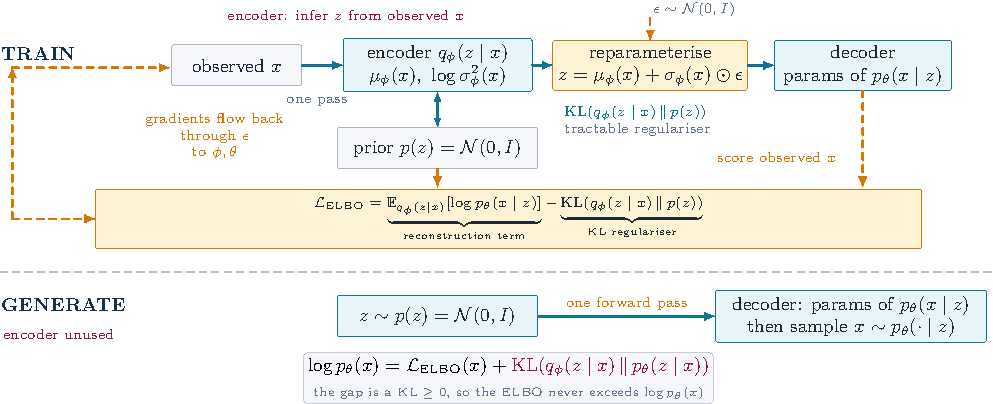
\includegraphics[width=\textwidth]{vae_architecture.pdf}
\caption{VAE 的训练与生成路径。左侧训练路径使用 encoder 得到 \(q_\phi(z\mid x)\)，随机性经重参数化 \(z=\mu+\sigma\odot\epsilon\) 引入，使梯度可以沿采样路径回传到 encoder；ELBO 的第一项是在 decoder 给出的条件分布下评价已观测 \(x\) 的对数概率，再减去 \(\KL(q_\phi(z\mid x)\Vert p(z))\)。右侧无条件生成路径从先验 \(p(z)=\mathcal N(0,I)\) 采样 \(z\)，由 decoder 输出观测分布 \(p_\theta(x\mid z)\) 的参数，再从中采样 \(x\)。ELBO 与真实 \(\log p_\theta(x)\) 之间的间隙正是 \(\KL(q_\phi(z\mid x)\Vert p_\theta(z\mid x))\)。}
\label{fig:vae-architecture}
\end{figure}

\subsection{离散潜变量：VQ-VAE}
\label{sec:vector-quantized-latents}

前面的高斯 VAE 用连续向量表示潜变量，但图像、语音和视频也可以先压缩成有限词表中的编号，再用离散序列模型学习这些编号的分布。例如，把一张图像编码成较小的二维编号网格，既能避开逐像素生成的长序列，又能把生成问题交给自回归 Transformer。向量量化变分自编码器（Vector-Quantized Variational Autoencoder，VQ-VAE）提供了这种从连续数据到离散潜变量的接口~\cite{vandenOord2017vqvae}。

设编码器在位置 \(i\) 输出 \(z_{e,i}(x)\in\R^d\)，可学习的码本为 \(\mathcal C=\{e_1,\ldots,e_M\}\subset\R^d\)。量化器选出最近的码字，用它代替编码器输出送入解码器：
\begin{equation}
 k_i(x)=\argmin_{1\leq j\leq M}\|z_{e,i}(x)-e_j\|_2^2,
 \qquad z_{q,i}(x)=e_{k_i(x)}.
 \label{eq:vq-lookup}
\end{equation}
例如，图像经过下采样编码器后得到 \(H'\times W'\) 个向量，每个位置执行一次式 \eqref{eq:vq-lookup}，便得到同样大小的整数索引网格 \((k_i)\)。每个整数 \(k_i\) 指向码本中的一个向量 \(e_{k_i}\)；把取出的向量按原来的空间位置排列，解码器便可据此重构图像。

训练的难点在于最近邻选择。只要 \(z_{e,i}\) 没有越过两个码字的分界面，\(z_{q,i}\) 就保持不变，因此量化映射对 \(z_{e,i}\) 的真实导数几乎处处为零，在分界面上不可导。VQ-VAE 采用直通估计（Straight-Through Estimator，STE）：用 \(\perp(u)\) 表示停止梯度操作，它在前向计算时等于 \(u\)，反向计算时对 \(u\) 的导数记为零。令
\begin{equation}
 \widetilde z_{q,i}=z_{e,i}+\perp(z_{q,i}-z_{e,i}).
 \label{eq:vq-straight-through}
\end{equation}
前向计算时 \(\widetilde z_{q,i}=z_{q,i}\)，解码器看到的仍是离散码字；反向计算时却规定 \(\partial\widetilde z_{q,i}/\partial z_{e,i}=I\)，把重构损失对解码器输入的梯度直接传给编码器。即使量化结果在一个邻域内完全不变，这个规则仍按单位导数回传。确定性的最近邻选择也没有可直接代入 score-function 公式的随机类别抽样分布。STE 是有意替换导数的工程折中，能帮助训练。

梯度直接传给编码器还不足以训练码本，因为式 \eqref{eq:vq-straight-through} 中的重构项不会沿这条路径更新 \(e_{k_i}\)。码本里的候选向量 \(e_1,\ldots,e_M\) 本身也是可训练参数；一种常用目标为
\begin{equation}
\begin{aligned}
 \mathcal J_{\mathrm{VQ}}(x)
 ={}&-\log p_\theta(x\mid\widetilde z_q)
 +\sum_i\|\perp(z_{e,i})-e_{k_i}\|_2^2\\
 &+\beta\sum_i\|z_{e,i}-\perp(e_{k_i})\|_2^2.
\end{aligned}
\label{eq:vq-loss}
\end{equation}
第一项更新解码器，并通过直通梯度更新编码器；第二项只更新本次被选中的码本向量，把它们拉向对应的编码器输出；第三项称为 commitment loss，只更新编码器，让输出靠近所选码字，\(\beta>0\) 控制其强度。码本向量也可以用编码器输出的移动平均更新。整数索引 \(k_i\) 不直接参与梯度更新，但编码器和码本向量改变后，下一次前向传播选中的索引可能随之改变。

离散变量也可以有 KL 散度：若 \(q_j,p_j\) 是两组类别概率，则 \(\KL(q\Vert p)=\sum_j q_j\log(q_j/p_j)\)。但这里的最近邻选择给出确定性的后验 \(q(k_i\mid x)\)：一个编号的概率为 1，其余为 0。若第一阶段暂取均匀先验 \(p(k_i)=1/M\)，则每个位置的 \(\KL(q(k_i\mid x)\Vert p(k_i))=\log M\) 是常数，不提供训练梯度。式 \eqref{eq:vq-loss} 后两项约束的是编码器输出与所选码字之间的距离，作用不同于高斯 VAE 中匹配后验与先验的 KL 项。

式 \eqref{eq:vq-loss} 的训练始终从真实图像 \(x\) 出发：编码器为各位置选出索引 \(k_i(x)\)，解码器利用对应的码本向量重构这张图像。若要不输入图像、从零生成新图像，就不能依靠编码器提供索引；此时还需要一个模型来决定每个位置该选哪个编号，以及不同位置的编号如何搭配。

为此，先用训练好的编码器把训练集中的每张图像变成索引网格，再按固定顺序读成序列。例如，\(2\times2\) 的网格 \(\bigl(\begin{smallmatrix}7&42\\3&19\end{smallmatrix}\bigr)\) 按行读成 \((7,42,3,19)\)。用这些真实图像产生的序列训练自回归 Transformer：给定前面的编号，预测下一个编号，并用真实编号计算交叉熵。这个索引序列的概率模型记为 \(p_\psi(k_1,\ldots,k_N)\)，其中 \(N=H'W'\)。生成时依次采样 \(N\) 个编号，按原顺序排回网格，把每个编号 \(k_i\) 换成码本向量 \(e_{k_i}\)，最后由已训练的解码器生成图像。

\Needspace{8\baselineskip}
\section{可逆流、对抗生成与能量模型}

\subsection{Normalizing Flow}

前面的高斯 VAE 需要对潜变量积分，使边缘似然难以精确计算。如果把数据与基分布之间的映射限制为同维、可逆的变换，就可以逐点追踪概率密度如何变化，并通过逆变换直接生成样本。这是下面可逆流模型的出发点。

Normalizing Flow 是一串可逆、可微的变换~\cite{papamakarios2021normalizing}。令 \(x\) 是数据空间中的样本，\(z=f_\theta(x)\) 是它在简单基分布中的坐标，例如 \(p_Z(z)=\mathcal N(0,I)\)。变量变换公式为
\begin{equation}
 \log p_X(x)=\log p_Z(f_\theta(x))+\log\left|\det\frac{\partial f_\theta(x)}{\partial x}\right|.
\end{equation}
如果直接用任意神经网络表示 \(f_\theta\)，它虽然可能有很强的表达能力，但既不一定可逆，也需要计算一个 \(d\times d\) Jacobian 的行列式。RealNVP 用 affine coupling layer 解决这两个问题~\cite{dinh2016density}。把输入按 mask 分成 \(x=(x_a,x_b)\)，第一部分直接复制，第二部分由第一部分产生 scale 和 shift：
\begin{align}
 z_a&=x_a,\\
 z_b&=x_b\odot\exp s_\theta(x_a)+t_\theta(x_a).
\end{align}
这里 \(s_\theta,t_\theta\) 可以是普通的卷积网络或多层感知机，它们本身不需要可逆；可逆性来自 \(x_b\) 只做逐元素的仿射变换。逆变换可以显式写出：
\begin{equation}
 x_a=z_a,\qquad
 x_b=\left(z_b-t_\theta(z_a)\right)\odot\exp[-s_\theta(z_a)].
\end{equation}

它能快速计算 Jacobian，是因为矩阵具有块三角结构：
\begin{equation}
 \frac{\partial z}{\partial x}
 =
 \begin{bmatrix}
 I & 0\\
 \frac{\partial z_b}{\partial x_a}
 & \operatorname{diag}\!\left(\exp s_\theta(x_a)\right)
 \end{bmatrix},
 \qquad
 \log|\det J|=\sum_j s_{\theta,j}(x_a).
\end{equation}
行列式只等于对角线元素的乘积，不需要对完整 Jacobian 做 \(O(d^3)\) 的通用行列式计算；在多层 coupling layer 中，log-determinant 只是每层 scale 输出的求和。不同层交替 mask，使前一层没有改变的 \(x_a\) 在下一层成为被变换的部分，否则模型会永久保留一半输入不变。

Flow 的训练目标是真实数据的精确负对数似然：
\begin{equation}
 \mathcal L_{\mathrm{Flow}}
 =-\frac1N\sum_i\left[
 \log p_Z(f_\theta(x^{(i)}))
 +\log|\det J_{f_\theta}(x^{(i)})|
 \right].
\end{equation}
训练时把数据 \(x\) 经过各层正向变换得到 \(z\)，基分布 log-density 和每层 log-determinant 都能反向传播到 \(s_\theta,t_\theta\)。前向训练不需要从模型中抽样，也没有 VAE 那样的潜变量积分；生成时才从 \(z\sim p_Z\) 随机采样，再按相反顺序运行显式逆变换得到 \(x\)。因此 Flow 同时有精确 likelihood、可逆编码和直接采样，但它必须牺牲一部分任意神经网络的自由度来保证可逆性；高维数据的多尺度分解、边界处理、scale 爆炸和层数带来的逆向成本都是主要架构难点。

\begin{figure}[H]
\centering
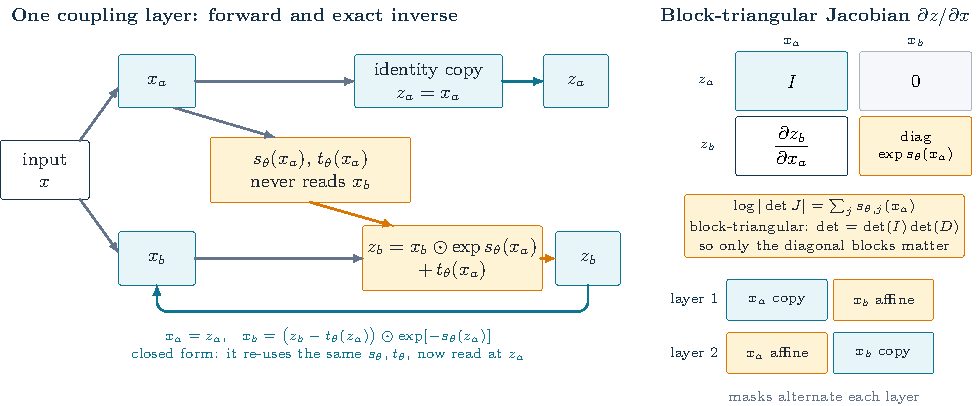
\includegraphics[width=\textwidth]{realnvp_architecture.pdf}
\caption{RealNVP coupling layer 的正向与逆向计算。复制分支把 \(x_a\) 原样送出，scale/shift 网络只读取 \(x_a\) 并产生逐元素仿射参数，因此 \(x_b\) 的变换是逐元素的，整个映射可以显式求逆。右侧的块三角 Jacobian 说明行列式只等于对角块 \(\operatorname{diag}(\exp s_\theta(x_a))\) 的乘积，log-determinant 退化为 \(\sum_j s_{\theta,j}(x_a)\)，无需 \(O(d^3)\) 的通用行列式计算。相邻层交换 mask 划分，避免一半输入始终不变。}
\label{fig:realnvp-architecture}
\end{figure}

\subsection{连续归一化流：神经常微分方程（Neural ODE）与密度演化}
\label{sec:cnf}

RealNVP 通过有限层变换逐层累加 log-determinant。另一种做法是把层间更新写成 \(x_{k+1}=x_k+\Delta r\,v_\theta(x_k,r_k)\)，并在 \(\Delta r\to0\) 时用连续时间 \(r\in[0,1]\) 描述从基分布到数据分布的运动：
\begin{equation}
 \frac{dx_r}{dr}=v_\theta(x_r,r),\qquad x_{r=0}=z\sim p_0.
 \label{eq:cnf-ode}
\end{equation}
用神经网络表示微分方程右侧的速度场，并通过数值求解器积分得到 \(x_1\)，这就是 Neural ODE 的基本计算路径~\cite{chen2018neuralode}。训练时还要计算损失对 \(\theta\) 的梯度：可以让自动微分穿过数值积分的各步，也可以使用伴随灵敏度方程。因而 Neural ODE 把“解微分方程得到输出”与“梯度能穿过求解过程”放在同一模型中；积分步数和梯度计算方式决定实际训练成本。

当这条 ODE 用于概率建模时，还需要追踪运动中的密度，这样的模型称为连续归一化流~\cite{chen2018neuralode,grathwohl2019ffjord}。样本沿式 \eqref{eq:cnf-ode} 运动时，概率质量守恒给出连续性方程 \(\partial_r p_r=-\nabla\cdot(p_rv_\theta)\)。沿单条轨迹使用链式法则，得到瞬时变量变换公式
\begin{equation}
 \frac{d}{dr}\log p_r(x_r)
 =-\nabla\cdot v_\theta(x_r,r)
 =-\operatorname{tr}\!\left(\frac{\partial v_\theta}{\partial x}(x_r,r)\right).
 \label{eq:cnf-density}
\end{equation}
因此，从 \(z=x_{r=0}\) 积分到 \(x=x_{r=1}\) 时，\(\log p_1(x)=\log p_0(z)-\int_0^1\nabla\cdot v_\theta(x_r,r)\,dr\)。生成只需从 \(p_0\) 抽样并向前积分；评价给定数据 \(x\) 的密度则从 \(x_{r=1}=x\) 反向积分到 \(z\)，同时累积散度。与有限层变换中的 Jacobian 行列式相比，连续时间的局部体积变化由迹表示：\(\log\det(I+\Delta r J)=\Delta r\operatorname{tr}J+O(\Delta r^2)\)。速度网络因而可以采用较自由的结构；在保证 ODE 解唯一性的常规条件下，正向与反向积分给出互逆映射。

若直接用 \(-\log p_1(x)\) 训练 CNF，每次更新都要数值求解状态和散度的积分，再把梯度传回速度网络。迹的计算在高维时仍有代价，可用迹估计等方法处理；数值求解精度也影响最终的密度值。后面的 Flow Matching 将保留同一个生成 ODE，改用已知概率路径的速度作为训练标签。

\subsection{生成对抗网络}
\label{sec:gan}

如果任务重点是快速产生逼真的样本，可以放松对显式似然的要求，让一个辅助网络判断生成结果与真实数据的差别，再把这种反馈传给生成器。这样生成网络能采用更自由的结构，训练则需要协调两个网络。

GAN 用生成器 \(G_\theta(z)\) 把简单噪声 \(z\sim p_Z\) 推送成样本，用判别器 \(D_\phi(x)\in(0,1)\) 判断输入来自真实数据还是生成器~\cite{goodfellow2014gan}。原始 minimax 目标是
\begin{equation}
 \min_\theta\max_\phi V(D_\phi,G_\theta)
 =\E_{x\sim p_{\mathrm{data}}}\log D_\phi(x)
 +\E_{z\sim p_Z}\log\left[1-D_\phi(G_\theta(z))\right].
\end{equation}
对固定的生成分布 \(p_g\)，若判别器有无限容量且达到最优，它在每个 \(x\) 上的解为
\begin{equation}
 D^*(x)=\frac{p_{\mathrm{data}}(x)}
 {p_{\mathrm{data}}(x)+p_g(x)}.
\end{equation}
把 \(D^*\) 代回目标后，生成器的目标可写成 Jensen--Shannon 散度（Jensen--Shannon Divergence，JSD）：
\begin{equation}
 V(D^*,G)=-\log 4+
 2\,\operatorname{JSD}\!\left(p_{\mathrm{data}}\Vert p_g\right),
\end{equation}
JSD 是对称散度，其值在两个分布一致时为零。理想 Nash equilibrium 的含义是 \(p_g=p_{\mathrm{data}}\)，此时 \(D^*(x)=1/2\)，判别器无法从样本判断真假，生成器也没有方向继续改善；这个平衡在无限数据、无限模型容量和全局最优的设定下成立，有限网络的交替训练是它的近似。

实践中每一步先固定 \(G\) 更新判别器，再固定 \(D\) 更新生成器。原始生成器损失 \(\E_z\log[1-D(G(z))]\) 在判别器很强时容易梯度饱和：若生成样本很容易被识别，\(D(G(z))\approx0\)，判别器末端 sigmoid 已落在接近水平的区域，链式法则传回生成器的梯度因而接近零。这里的“饱和”指的是原始生成器目标在当前参数区间几乎不给出可用的改进方向。因此交替训练时常用 non-saturating loss
\begin{equation}
 \mathcal L_G^{\mathrm{non\text{-}saturating}}=-\E_{z\sim p_Z}\log D_\phi(G_\theta(z)).
\end{equation}
它与 minimax 目标拥有相同的理想平衡点，区别在于梯度从哪个方向进入。原始生成器目标对生成器参数的梯度是
\begin{equation}
 \nabla_\theta\E_z\log[1-D(G(z))]=-\E_z\frac{\nabla_\theta D(G(z))}{1-D(G(z))},
\end{equation}
当 \(D(G(z))\approx0\) 时分母接近 \(1\)，梯度量级较小；而 non-saturating 损失的梯度是
\begin{equation}
 \nabla_\theta\left[-\E_z\log D(G(z))\right]=-\E_z\frac{\nabla_\theta D(G(z))}{D(G(z))},
\end{equation}
此时分母接近 \(0\)，梯度被放大。也就是说，判别器越确信生成样本是假的，non-saturating 损失给出的更新方向反而越强，而原始 minimax 形式的生成器梯度则趋于消失。代价是 non-saturating 损失在生成器已经能骗过判别器时权重变小，学习信号随之减弱；两者的平衡点相同，梯度在训练不同阶段的有效性不同。

GAN 的生成器需要对自己产生的样本求导：噪声 \(z\sim p_Z\) 与 \(\theta\) 无关，给定 \(z\) 后，梯度沿 \(z\to G_\theta(z)\to D_\phi(G_\theta(z))\) 回传。这是第 \ref{sec:gradient-estimator-map} 节的路径梯度；由于输入噪声已经固定分布，不需要再做 VAE 式的重参数化。GAN 不显式计算 \(p_g(x)\) 或 likelihood，推理时只需一次 \(G_\theta\) 前向传播，代价低；训练却是非凸的双层博弈，判别器过强、梯度不平衡和 mode collapse 会使生成器只覆盖少数容易骗过判别器的模式。图 \ref{fig:gan-architecture} 画出两步交替更新的数据流和梯度路径：判别器步只更新 \(\phi\)；生成器步固定 \(D_\phi\)，梯度穿过判别器和生成样本回到 \(G_\theta\)。

\begin{figure}[ht]
\centering
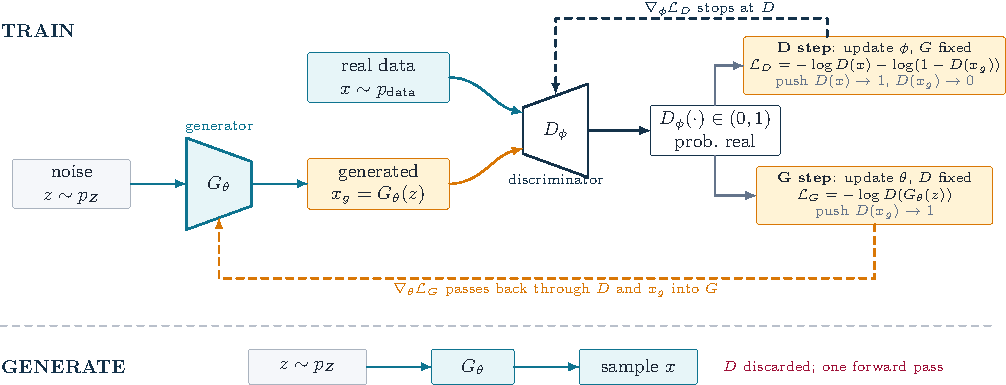
\includegraphics[width=\textwidth]{gan_architecture.pdf}
\caption{GAN 的网络结构与交替训练。生成器 \(G_\theta\) 把噪声 \(z\) 映成样本 \(x_g\)，判别器 \(D_\phi\) 对真实样本和生成样本输出“为真”的概率。判别器步固定 \(G\)，用 \(\mathcal L_D\) 更新 \(\phi\)；生成器步固定 \(D\)，用 non-saturating 损失 \(\mathcal L_G\) 更新 \(\theta\)，梯度经 \(D\) 与 \(x_g\) 回到 \(G\)。生成时丢弃判别器，只做一次生成器前向。}
\label{fig:gan-architecture}
\end{figure}

\begin{figure}[ht]
\centering
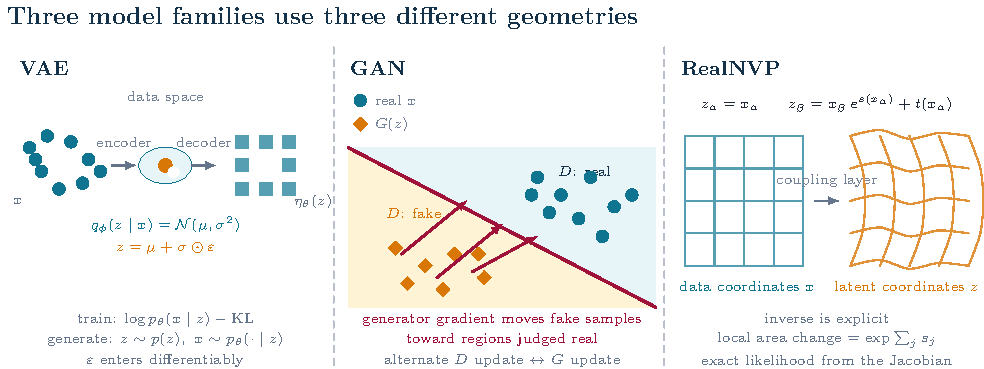
\includegraphics[width=\textwidth]{vae_gan_realnvp_networks.pdf}
\caption{VAE、GAN 和 RealNVP 的神经网络与梯度路径对照。VAE 面板的像素网格表示 decoder 输出的观测分布参数 \(\eta_\theta(z)\)，具体样本还需从该分布抽取；VAE 的随机性通过 \(\epsilon\) 进入可微重参数化。GAN 的生成器通过判别器损失获得梯度；RealNVP 通过耦合层的显式逆变换和三角 Jacobian 保持可逆。}
\label{fig:generative-network-comparison}
\end{figure}

\subsection{核匹配与量子线路 Born machine}

GAN 说明，即使难以逐点计算 \(p_\theta(x)\)，只要能够从模型采样，仍可用真实样本和生成样本训练模型。另一条训练路径是直接比较两组样本的统计量。经典的生成矩匹配网络（Generative Moment Matching Network，GMMN）使用最大均值差异（Maximum Mean Discrepancy，MMD）作为生成损失~\cite{li2015gmmn,gretton2012kernel}。

给定正定核函数 \(k(x,y)=\langle\phi(x),\phi(y)\rangle_{\mathcal H_k}\)，核技巧允许我们通过样本对上的 \(k(x,y)\) 比较特征均值，而不必显式构造可能无限维的特征映射 \(\phi\)。其平方损失为
\begin{align}
 \mathcal L_{\mathrm{MMD}}(\theta)
 &=\left\|\E_{x\sim p_{\mathrm{data}}}\phi(x)-\E_{y\sim p_\theta}\phi(y)\right\|_{\mathcal H_k}^{2}\notag\\
 &=\E_{x,x'\sim p_{\mathrm{data}}}k(x,x')
 +\E_{y,y'\sim p_\theta}k(y,y')
 -2\E_{x\sim p_{\mathrm{data}},\,y\sim p_\theta}k(x,y).
\end{align}
其中 \(x,x'\) 和 \(y,y'\) 分别是各自分布中的独立样本；三个期望都可以用两个样本批次中的样本对估计。例如，连续向量可用高斯核，比特串可用基于汉明距离的核；核的选择决定训练时关注哪些样本差别。对于能区分分布的特征核，理论上 \(\operatorname{MMD}(p,q)=0\) 当且仅当 \(p=q\)。

从“用测试函数区分两组样本”的角度看，MMD 可以直观地理解为一种限制了判别方式的 GAN：它把测试函数限制在预先选定的核函数空间的单位球内，取两组样本在这些函数上的最大期望差；GAN 则训练判别网络来学习区分特征。这个类比只说明训练信号的来源；原始 GAN 的目标对应理想条件下的 Jensen--Shannon 散度，MMD 则是核函数空间中的分布距离。固定核省去了交替优化，目标较直接；但在高维数据中，基于距离的核及其宽度未必反映有用的结构，过宽的核会抹平差别，过窄的核又可能让两组样本之间几乎没有训练信号。对大小为 \(B\) 的批次，直接计算经验 MMD 还需 \(O(B^2)\) 个样本对核值。GAN 的可学习判别器能够适应复杂特征，却引入博弈不稳定和模式缺失的风险；若让网络学习 MMD 所用的特征，也会重新引入类似的对抗优化~\cite{li2017mmdgan}。

量子线路 Born machine（Quantum Circuit Born Machine，QCBM）展示了用参数化量子线路构造生成器的方法~\cite{liu2018qcbm}。参数化线路 \(U_\theta\) 制备量子态，对 \(n\) 个量子比特测量即可得到比特串 \(x\in\{0,1\}^n\)，其概率由 Born 规则定义为
\begin{equation}
 p_\theta(x)=\left|\langle x|U_\theta|0^n\rangle\right|^2.
\end{equation}
采样只需运行并测量线路；要从有限测量次数高精度估计某个稀有比特串的相对概率则很昂贵。于是可以直接把真实比特串与测量结果放进上面的 MMD 损失，而不计算逐点似然。经典 GMMN 需要对生成样本上的核函数求导，可沿可微生成器使用第 \ref{sec:gradient-estimator-map} 节的路径梯度；QCBM 的离散测量结果没有这条梯度路径，训练常对可移位参数门使用参数移位规则，运行偏移参数的线路来估计损失梯度。因此“容易采样”解决了损失评估所需的模型样本，参数优化仍需多次线路运行。QCBM 是按 Born 规则定义分布，与下节按能量和配分函数定义分布的 Boltzmann machine 不同。

\subsection{能量模型与 MCMC}
\label{sec:ebm-mcmc}

有些任务很容易判断一个构型是否合理，却很难直接给出它的归一化概率。例如，物理哈密顿量能为每个构型计算能量，但平衡分布的配分函数需要遍历整个构型空间。能量模型沿用这一思路：先给样本打能量分数，再解决归一化与采样。

EBM（Energy-Based Model，能量模型）用一个能量函数 \(E_\theta(x)\) 规定一条未归一化密度：
\begin{equation}
 p_\theta(x)=Z_\theta^{-1}\exp[-E_\theta(x)],\qquad
 Z_\theta=\int\exp[-E_\theta(x)]\,dx.
\end{equation}
\(E_\theta\) 可以是任意标量函数，灵活度高于显式密度模型；物理中“能量越低概率越高”的先验也可以直接写进 \(E_\theta\)。代价全部落在配分函数 \(Z_\theta\) 上：它是对整个 \(x\) 空间的积分，除极少数特例都无法解析计算，而 \(Z_\theta\) 同时出现在归一化、采样和训练梯度三个地方。训练梯度可以把它约掉，采样也能在不知道 \(Z_\theta\) 的情况下进行。

\textbf{最大似然的参数梯度。}把 \(\log p_\theta(x)=-E_\theta(x)-\log Z_\theta\) 对 \(\theta\) 求导，第一项直接给出 \(-\nabla_\theta E_\theta(x)\)，第二项需要处理 \(Z_\theta\) 对参数的依赖。关键事实是：虽然 \(Z_\theta\) 本身算不出来，它的对数梯度却可以写成对模型分布取期望的形式，
\begin{align}
 \nabla_\theta\log Z_\theta
 &=\frac{1}{Z_\theta}\nabla_\theta\int\exp[-E_\theta(x)]\,dx
 =\frac{1}{Z_\theta}\int-\nabla_\theta E_\theta(x)\exp[-E_\theta(x)]\,dx\notag\\
 &=-\int p_\theta(x)\nabla_\theta E_\theta(x)\,dx
 =-\E_{p_\theta}[\nabla_\theta E_\theta(x)].
\end{align}
第二个等号把梯度移进积分，第三个等号把 \(\exp[-E_\theta]/Z_\theta\) 整体识别成 \(p_\theta(x)\)。右端不用显式求出 \(Z_\theta\)，但仍需得到服从模型分布的样本，才能估计这个期望。把两项合起来并对数据取期望，
\begin{equation}
 \nabla_\theta\mathcal L_{\mathrm{NLL}}
 =\underbrace{\E_{p_{\mathrm{data}}}[\nabla_\theta E_\theta(x)]}_{\text{positive phase}}
 -\underbrace{\E_{p_\theta}[\nabla_\theta E_\theta(x)]}_{\text{negative phase}}.
\end{equation}
第一项只在真实数据上求值，实现简单，作用是降低数据点的能量；第二项要求在模型自身分布 \(p_\theta\) 上取期望，无法解析计算，只能采样。正负相位的名称来自统计物理中玻尔兹曼机的用法：负相位是把已建立的“模型样本能量”推高，使得模型不能靠把所有能量都压低来退化解。所以 EBM 的训练困难不在梯度公式，而在于每一步参数更新前都要先运行一次采样。

第 \ref{sec:gradient-estimator-map} 节讨论了如何对参数化抽样目标求导；这里的模型期望已由 \(\nabla_\theta\log Z_\theta\) 的解析求导得到，MCMC 只负责取得负相位样本，不需要对马尔可夫链的抽样步骤求导。

\textbf{用 MCMC 采样负相位。}目标是构造一条马尔可夫链，使其平稳分布恰好是 \(p_\theta\)，从而在链运行足够久之后把它当作 \(p_\theta\) 的样本。

Metropolis--Hastings（MH）从当前状态 \(x\) 按提议分布 \(q(x'\mid x)\) 抽一个候选 \(x'\)。其接受概率为
\begin{equation}
 a(x'\mid x)=\min\left\{1,\ \frac{\tilde p_\theta(x')q(x\mid x')}{\tilde p_\theta(x)q(x'\mid x)}\right\}.
\end{equation}
这里 \(\tilde p_\theta(x)=\exp[-E_\theta(x)]\) 是未归一化密度。接受率只用到未归一化密度的比值，\(Z_\theta\) 在分子分母同时出现并约掉，这就是 MCMC 绕开配分函数的机制。可以验证该接受率满足细致平衡 \(\tilde p_\theta(x)q(x'\mid x)a(x'\mid x)=\tilde p_\theta(x')q(x\mid x')a(x\mid x')\)，对 \(x\) 积分即得 \(p_\theta\) 是平稳分布。

Gibbs sampling 是 MH 的一个特例：当某个变量的条件分布在其余变量给定时可以精确采样时，直接从这个条件分布抽新值，接受率恒等于 \(1\)。它在 EBM 上能否使用取决于能量函数的结构。下面的受限玻尔兹曼机（RBM, Restricted Boltzmann Machine）就是一个条件分布可以精确计算的特例，它的例子把上面的正相位、负相位和持续链落成可执行步骤。

Langevin dynamics 用能量梯度构造新的候选状态 \(x'\)，适用于 \(E_\theta\) 可微的连续变量。连续时间形式是
\begin{equation}
 dx=-\tfrac12\nabla_x E_\theta(x)\,dt+dW_t,
\end{equation}
其中 \(W_t\) 是标准布朗运动，增量 \(dW_t\) 在时长 \(dt\) 内的协方差为 \(I\,dt\)。把它按步长 \(\eta\) 离散，就得到正文使用的迭代
\begin{equation}
 x_{k+1}=x_k-\frac{\eta}{2}\nabla_x E_\theta(x_k)+\sqrt{\eta}\,\xi_k,\qquad \xi_k\sim\mathcal N(0,I),
 \label{eq:langevin-step}
\end{equation}
它由“沿能量梯度下坡”和“热噪声扩散”两部分组成，噪声使链有机会离开局部极小值。这样构造为什么正确，可以用 Fokker--Planck 方程验证：该随机微分方程对应的密度演化方程是
\(\partial_t p=\tfrac12\nabla\cdot\bigl(p\nabla E_\theta+\nabla p\bigr)\)，代入 \(p\propto\exp(-E_\theta)\) 后括号内两项恰好抵消，右端为零，因此 \(p_\theta\) 正是它的平稳分布。在常见的光滑性和稳定性条件下，这种离散化会产生随步长变化的平稳分布偏差：直接使用上式是不加校正的 Langevin 算法，步长有限时采样分布偏离 \(p_\theta\)。把 Langevin 提议放进上面的 MH 接受/拒绝步骤，偏差被消除，得到带 Metropolis 接受校正的 Langevin 算法；代价是每步要评估候选点的能量与梯度以计算接受率，而步长 \(\eta\) 的选取同时影响探索状态空间的速度与偏差大小。这解释了它与 MCMC 的关系：Langevin 动力学提供一种梯度引导的采样机制；有限步长时可用 MH 校正保持目标平稳分布，也可接受不校正的离散化偏差。

即使采样方法以 \(p_\theta\) 为平稳分布，有限步的链也未必已接近它。这里的 mixing（混合）指马尔可夫链忘记初值并在各个高概率模式之间按目标权重移动的速度；若链只在一个能量谷附近来回，即使步数很多，得到的仍是高度相关且有偏的负样本。

\textbf{负相位的两种近似。}精确估计负相位要求样本服从 \(p_\theta\)，而训练时每个 minibatch 都要重算一次负相位，等待链充分混合的代价过高。常见做法是接受一个有偏但便宜的估计。

CD-\(k\)（Contrastive Divergence，\(k\) 步对比散度）从真实数据点出发，只跑 \(k\) 步 Gibbs 或 Langevin，用短链终点作为负样本，\(k\) 在实践中常取 \(1\)。它的更新量是“数据点的能量梯度减短链终点的能量梯度”。起点在数据附近使链不必先 burn-in，代价是终点尚未收敛到 \(p_\theta\)，因此所得更新带有短链偏差，主要探测数据附近模型赋予过高概率的区域，属于局部近似，不能保证覆盖所有模式。

PCD（Persistent Contrastive Divergence，持续对比散度）把上一条链的终点保存下来，作为下一次参数更新时链的起点，从而不必每轮重新 burn-in。风险是参数在链还未平衡时已经改变，链追踪的是一个持续移动的分布；若能量面存在相距很远的模式，链可能长期停在其中一个模式，负样本的分布因此系统性偏离 \(p_\theta\)。实务中需要监控多链的能量、自相关时间和跨模式跃迁。

\begin{examplebox}[RBM：一个能看见 Gibbs 更新细节的 EBM]
RBM 把二值可见变量 \(v\) 和隐藏变量 \(h\) 的能量写成
\begin{equation}
E(v,h)=-a^\mathsf Tv-b^\mathsf Th-v^\mathsf TWh.
\end{equation}
“受限”表示同一层内没有连接，因此 \(p(h_j=1\mid v)=\sigma(b_j+W_{:j}^\mathsf Tv)\) 和 \(p(v_i=1\mid h)=\sigma(a_i+W_{i:}h)\) 都可并行采样。一次 PCD 更新就是：保存 \(v^-\)，交替采样 \(h^-\sim p(h\mid v^-)\)、\(v^-\sim p(v\mid h^-)\) 若干步，用数据对 \((v^+,h^+)\) 与模型对 \((v^-,h^-)\) 的相关量之差更新 \(W\)，再把新的 \(v^-\) 留给下一轮。这个例子把“负相位”“持续链”和“混合”落实成了可执行步骤。
\end{examplebox}

训练之外，推理时 EBM 同样没有闭式前向采样，生成一个样本仍需运行许多 MCMC 步，因此采样速度和跨模式移动能力是它的核心限制。

\textbf{用得分匹配替代负相位采样。}当数据连续、密度足够光滑时，可以学习密度在每个数据点附近如何变化。得分函数（score）定义为 \(s_\theta(x)=\nabla_x\log p_\theta(x)\)：它是一个与 \(x\) 同维的向量，指向局部对数密度上升最快的方向。对能量模型，\(s_\theta=-\nabla_xE_\theta\)，因为配分函数对输入 \(x\) 是常数。得分匹配（score matching）最初就是为未归一化密度提出的~\cite{hyvarinen2005score}；它希望最小化
\begin{equation}
 J(\theta)=\frac12\int p(x)\|s_\theta(x)-\nabla_x\log p(x)\|^2\,dx,
 \label{eq:score-matching-target}
\end{equation}
这里 \(p=p_{\mathrm{data}}\) 表示数据的光滑总体密度。真实 score 未知，但结论可以先说：经分部积分，这个目标只差一个常数地等于 \(\E_p[\tfrac12\|s_\theta\|^2+\nabla\cdot s_\theta]\)，只需在数据样本上计算模型 score 及其散度，既不需要真实 score，也不需要负样本。推导分三步。

首先展开平方，并把与 \(\theta\) 无关的真实 score 平方项记为常数 \(C\)：
\begin{align}
 J(\theta)&=\frac12\E_p\|s_\theta\|^2-\int p(x)s_\theta(x)\cdot\nabla\log p(x)\,dx+C\\
 &=\frac12\E_p\|s_\theta\|^2-\sum_{j=1}^{d}\int s_{\theta,j}(x)\,\partial_jp(x)\,dx+C.
\end{align}
第二步只用了 \(p\,\partial_j\log p=\partial_jp\)。对每个坐标做分部积分，若边界项消失（例如无穷远处 \(p\,s_{\theta,j}\) 足够快趋零），则
\begin{equation}
 \int s_{\theta,j}\,\partial_jp\,dx
 =-\int p\,\partial_js_{\theta,j}\,dx.
\end{equation}
最后代回，交叉项的负号变成正号，得到
\begin{equation}
 J(\theta)=\E_p\!\left[\frac12\|s_\theta(x)\|^2+\nabla\cdot s_\theta(x)\right]+C,
 \label{eq:score-matching-computable}
\end{equation}
其中散度 \(\nabla\cdot s_\theta=\sum_j\partial_js_{\theta,j}\)；若 \(s_\theta=\nabla\log p_\theta\)，它就是 \(\log p_\theta\) 对输入的 Hessian 矩阵的迹。对由标量能量 \(E_\theta\) 定义的模型，把 \(s_\theta=-\nabla_xE_\theta\) 代入，实际最小化的样本平均是
\begin{equation}
 \widehat J(\theta)=\frac1B\sum_{i=1}^{B}\left[\frac12\|\nabla_xE_\theta(x_i)\|^2-\operatorname{tr}\!\left(\nabla_x^2E_\theta(x_i)\right)\right],
 \label{eq:ebm-score-matching-batch}
\end{equation}
省去了与 \(\theta\) 无关的常数。每个 \(x_i\) 都来自真实数据 minibatch，不需要从当前能量模型采负样本。第一项先前向计算标量 \(E_\theta(x_i)\)，再用自动微分对输入 \(x_i\) 求梯度，并把各坐标的梯度平方相加。第二项是同一能量函数对输入的 Hessian 对角线之和；低维时可逐坐标对 \(\partial_{x_j}E_\theta\) 再求一次 \(\partial_{x_j}\)，高维时这样做要计算许多二阶导数。

\Needspace{13\baselineskip}
高维的一个实用近似是为每个样本抽取若干独立随机向量 \(v_k\)，使 \(\E[v_kv_k^\mathsf T]=I\)，例如每个分量独立取 \(+1\) 或 \(-1\)。利用随机迹估计，
\begin{equation}
 \operatorname{tr}(\nabla_x^2E_\theta(x_i))
 =\E_v\!\left[v^\mathsf T\nabla_x^2E_\theta(x_i)v\right]
 \approx\frac1K\sum_{k=1}^{K}v_k^\mathsf T\nabla_x^2E_\theta(x_i)v_k.
\end{equation}
实际计算无需存下整个 Hessian：先求 \(g(x)=\nabla_xE_\theta(x)\)，再对标量 \(g(x)\cdot v_k\) 关于 \(x\) 求梯度，便得到 Hessian--向量积 \(\nabla_x^2E_\theta(x)v_k\)。将这两项的 minibatch 均值对参数 \(\theta\) 反向传播时，必须保留输入导数的计算图。随机迹估计省去逐坐标计算，但有抽样方差；切片得分匹配还将第一项投影到随机方向，已被用于训练深度能量模型~\cite{song2020sliced}。这种训练避免了负相位 MCMC，却要求能量函数能对输入稳定求导；下一节把目标放到带噪密度上，用已知噪声构造去噪回归，从而避免显式计算散度。

\subsection{按权重采样：生成流网络}
\label{sec:gflownet}

EBM 把目标写成 \(p(x)\propto e^{-E(x)}\)，采样留给马尔可夫链。若这个未归一化目标已经由外部给出，还可以把“构造 \(x\)”的过程学成一个策略：训练完成后，从初始状态一路采样到终止状态，得到一个样本；样本出现的频率正比于 \(R(x)\)。这类模型叫生成流网络（Generative Flow Network，GFlowNet）~\cite{bengio2021gflownet}。

这里的 \(R\) 是未归一化权重，目标分布是 \(p(x)=R(x)/Z\)。取 \(R(x)=e^{-\beta E(x)}\) 就得到玻尔兹曼分布，温度由 \(\beta\) 控制；取 \(R(x)=\exp(r(x)/\tau)\) 就得到第一章的 KL 倾斜解。后文沿用 GFlowNet 文献的“奖励”一词，但它在数学上始终是这条权重。

设状态图是一个有向无环图，从初始状态 \(s_0\) 出发，每步选择一个动作转移到下一个状态，终止状态就是样本 \(x\)。前向策略 \(P_F(s'\mid s)\) 决定怎样构造；反向策略 \(P_B(s\mid s')\) 只在训练时用来计算回流。一条完整轨迹 \(\tau=(s_0,\ldots,s_n=x)\) 的前向概率和反向概率分别是
\begin{equation}
 P_F(\tau)=\prod_{t=0}^{n-1}P_F(s_{t+1}\mid s_t),\qquad
 P_B(\tau\mid x)=\prod_{t=1}^{n}P_B(s_{t-1}\mid s_t).
 \label{eq:gfn-path-prob}
\end{equation}
给定终止状态的未归一化目标 \(R(x)\ge0\)，训练要让 \(P_F\) 满足下面的轨迹平衡。

\(P_F\) 和 \(P_B\) 都是可学习的概率函数，通常共用一个状态编码器和两个输出头。给定状态 \(s\) 的编码向量，前向头在从 \(s\) 出发的所有合法动作上做 softmax，得到 \(P_F(\cdot\mid s)\)；给定状态 \(s'\) 的编码向量，反向头在所有能一步到达 \(s'\) 的状态上做 softmax，得到 \(P_B(\cdot\mid s')\)。后者是 \(P_B\) 的另一种参数化：状态图里有几个前驱，就在这几个前驱之间分配概率。

两个头共享编码器、各自归一化，训练时一起更新；采样只调用前向头。状态是序列前缀时，编码器就是 Transformer 或 RNN；状态是集合或图时，换成对应的结构。若状态数很少，这些概率可以直接存成一张查表；它是网络的一个特例。反向策略也可以固定成均匀分布，这时只学 \(P_F\) 和 \(\log Z\)。

状态图的结构决定 \(P_B\) 要不要训练。自回归的生成树是一棵以 \(s_0\) 为根、每个节点只有一个父节点的树：给定当前状态 \(s'\)，能一步到达它的状态只有它的父节点，因此 \(P_B(s\mid s')=1\) 对所有边成立，反向头没有任何可学的参数，轨迹平衡里与 \(P_B\) 有关的项恒为零。反过来，当状态图是一般的 DAG——同一个状态可以由不同的构造顺序到达，例如按不同顺序选原子、或按不同顺序填格子——一个状态有多个前驱，\(P_B\) 才需要训练，用来把流量在几条汇入路径之间按比例分配。

先看一个长度为 2 的比特串的例子。\(x\) 取 \(00,01,10,11\) 之一，目标权重设为
\begin{equation}
 R(00)=1,\quad R(01)=3,\quad R(10)=3,\quad R(11)=9,
\end{equation}
则 \(Z=16\)，目标分布是 \((1,3,3,9)/16\)。构造从 \(s_0\) 开始，第一步选第一位，第二步选第二位，选完即终止；状态图是一棵二叉树，四条从 \(s_0\) 到叶子的路径对应四个样本。

\begin{figure}[H]
\centering
\begin{tikzpicture}[x=1cm,y=1cm,font=\small]
  \node[tealblock,minimum width=16mm] (s0) at (0,0) {$s_0$};
  \node[softblock,minimum width=11mm] (b0) at (2.6,1.4) {0};
  \node[softblock,minimum width=11mm] (b1) at (2.6,-1.4) {1};
  \node[softblock,minimum width=15mm] (x00) at (5.4,2.2) {00\\{\scriptsize $R=1$}};
  \node[softblock,minimum width=15mm] (x01) at (5.4,0.8) {01\\{\scriptsize $R=3$}};
  \node[softblock,minimum width=15mm] (x10) at (5.4,-0.8) {10\\{\scriptsize $R=3$}};
  \node[orangeblock,minimum width=15mm] (x11) at (5.4,-2.2) {11\\{\scriptsize $R=9$}};
  \draw[flow] (s0) -- node[above,font=\scriptsize]{0.5} (b0);
  \draw[flow,Orange,line width=1.1pt] (s0) -- node[below,font=\scriptsize]{0.5} (b1);
  \draw[flow] (b0) -- node[above,font=\scriptsize]{0.8} (x00);
  \draw[flow] (b0) -- node[below,font=\scriptsize]{0.2} (x01);
  \draw[flow] (b1) -- node[above,font=\scriptsize]{0.2} (x10);
  \draw[flow,Orange,line width=1.1pt] (b1) -- node[below,font=\scriptsize]{0.8} (x11);
\end{tikzpicture}
\caption{两步构造的例子。每条从 \(s_0\) 到叶子的路径是一条轨迹；边上的数字是当前的 \(P_F\)。橙色路径 \(s_0\to1\to11\) 的前向概率是 \(0.5\times0.8=0.4\)，终点权重 \(R(11)=9\)。树里每个非根状态只有一个前驱，因此 \(P_B\equiv1\)。}
\label{fig:gflownet-tree}
\end{figure}

图上边的数字是当前策略。取橙色轨迹 \(\tau=(s_0\to1\to11)\)，前向概率是 \(P_F(\tau)=0.5\times0.8=0.4\)，终点 \(x=11\)，\(R(x)=9\)。树里每个非根状态只有一个前驱，因此 \(P_B(1\mid11)=1\)、\(P_B(s_0\mid1)=1\)，\(P_B(\tau\mid x)=1\)。轨迹平衡要求
\begin{equation}
 Z\,P_F(\tau)=R(x)\,P_B(\tau\mid x),
 \label{eq:gfn-tb}
\end{equation}
其中 \(Z=\sum_xR(x)\) 是配分函数。把每条边想成一根水管：\(P_F\) 决定水往哪个分支流，\(P_B\) 描述从叶子往回看的分配；这个条件要求经过这条轨迹到达 \(x\) 的流量，等于 \(R(x)\) 分给这条轨迹的流量。四条路径都满足时，叶子 \(x\) 收到的总流量就是 \(R(x)\)，总流量是 \(Z\)。

训练时把两边取对数、移到同一侧，记残差
\begin{equation}
 \delta(\tau)=\log Z+\sum_{t=0}^{n-1}\log P_F(s_{t+1}\mid s_t)-\log R(x)-\sum_{t=1}^{n}\log P_B(s_{t-1}\mid s_t),
 \label{eq:gfn-residual}
\end{equation}
损失取 \(\mathcal L_{\mathrm{TB}}(\tau)=\delta(\tau)^2\)。\(\delta\) 的零点就是轨迹平衡成立的点，因此这个损失衡量的是流量约束的违反程度；它和最大似然的联系在下面单独说明。

\begin{examplebox}[一次训练更新]
\begin{enumerate}
  \item 从当前 \(P_F\) 采样一条轨迹 \(\tau\)，记终点为 \(x\)。
  \item 在终点读出 \(R(x)\)；若 \(R\) 来自模拟器或实验，只取这一个数。
  \item 计算 \(\log Z+\sum_t\log P_F-\log R(x)-\sum_t\log P_B\)，并把它的平方作为损失。
  \item 对损失反传，更新 \(\log Z\)、\(P_F\) 和 \(P_B\)。
\end{enumerate}
实际训练会并行采一批轨迹，并加 \(\epsilon\) 探索或温度，保证低概率分支也会被采到。
\end{examplebox}

\begin{table}[H]
\centering\small
\begin{tabularx}{\textwidth}{>{\bfseries}p{18mm} X X}
\toprule
量 & 训练时 & 采样时\\
\midrule
\(P_F\) & 采样轨迹，计算 \(\sum\log P_F\)，反传更新 & 每步按它抽一个动作\\
\(P_B\) & 计算 \(\sum\log P_B\)，反传更新；也可以固定成均匀分布 & 不使用\\
\(\log Z\) & 损失中的可学习标量，反传更新 & 直接读出\\
\(R(x)\) & 只在终点读一次数值 & 不使用\\
\bottomrule
\end{tabularx}
\caption{训练和采样各自用到哪些量。反向策略只在训练时出现。}
\label{tab:gfn-train-sample}
\end{table}

整个过程不需要负样本，也不需要 \(R\) 对 \(x\) 的梯度；\(R\) 只在一个终止状态上被读出。

\(\log Z\) 是一个单独的可学习标量，每个状态图只有一个，和网络参数一起通过梯度下降更新；它不进入 \(P_F\) 或 \(P_B\) 的计算。训练收敛后它的值就是 \(\log\sum_xR(x)\)，这也是 GFlowNet 能顺带估计配分函数的原因。

训练完成后，采样从 \(s_0\) 出发，每步按 \(P_F(\cdot\mid s)\) 抽一个动作，直到叶子。若训练后 \(P_F(1\mid s_0)=0.75\)、\(P_F(1\mid1)=0.75\)，采到 11 的概率就是 \(0.75\times0.75=0.5625=9/16\)，与目标一致；重复 \(N\) 次，各叶子出现的频率接近 \(R(x)/Z\)。采样时不需要计算 \(R\)，也没有马尔可夫链。条件生成把不合法动作的概率置零，或从固定前缀继续；\(\log Z\) 直接读训练好的标量。

轨迹平衡的目标和最大似然、score matching 是同一类约束的不同写法。若数据分布恰好是 \(p(x)=R(x)/Z\)，那么最小化 \(\KL(p\Vert p_\theta)\) 的最优解就是 \(p_\theta=p\)；GFlowNet 不从这个 KL 出发，而是直接要求 \(P_F\) 诱导的边缘分布等于 \(R/Z\)，等价于要求所有轨迹上的流量守恒。这也是它和 score matching 的分工：score matching 学的是 \(\nabla_x\log p(x)\)，GFlowNet 学的是能产生 \(p(x)\) 的构造过程。

轨迹平衡用整条轨迹作约束，一条长轨迹上 \(\delta\) 的方差会随长度累积。另外两种写法缩短了约束的范围。detailed balance 只约束一条边 \((s,s')\)：记 \(F(s)=Z\,P_F(s)\) 为经过状态 \(s\) 的总流量，
\begin{equation}
 F(s)P_F(s'\mid s)=F(s')P_B(s\mid s'),
\end{equation}
流入等于流出；它比轨迹平衡强，因为它要求每个中间状态都成立。sub-trajectory balance 介于两者之间，只约束一段子轨迹 \((s_k,\ldots,s_m)\)：
\begin{equation}
 F(s_k)\prod_{t=k}^{m-1}P_F(s_{t+1}\mid s_t)=F(s_m)\prod_{t=k}^{m-1}P_B(s_t\mid s_{t+1}),
\end{equation}
两端各用一个学到的流量 \(F\)，中间只用前向和反向策略。子轨迹越短，参与的因子越少，方差越低；取整条轨迹就退回轨迹平衡，取一条边就退回 detailed balance。

\begin{table}[H]
\centering\small
\begin{tabularx}{\textwidth}{>{\bfseries}p{24mm} X X}
\toprule
对比对象 & 相同 & 不同\\
\midrule
自回归 & 逐步构造，\(P_F\) 是逐位条件分布 & 自回归用最大似然拟合数据；GFlowNet 拟合给定的 \(R\)，状态图可以是集合、图或晶体\\
EBM & 目标都是未归一化密度 & EBM 用 MCMC 采样；GFlowNet 把采样学成一个前向策略\\
Flow Matching & 都在路径上匹配流量 & Flow Matching 的目标速度来自数据端点；GFlowNet 的目标流量来自终止状态的 \(R\)\\
KL 倾斜解 & 目标都可写成 \(p\propto p_0e^{r/\tau}\) & GFlowNet 不需要 \(p_0\) 的归一化，直接按 \(R\) 构造\\
策略梯度 & 都从策略采样 & 策略梯度最大化期望奖励；GFlowNet 让样本频率正比于 \(R\)\\
\bottomrule
\end{tabularx}
\caption{GFlowNet 与已有模型的对照。}
\label{tab:gflownet-relations}
\end{table}

GFlowNet 的目标比最大似然更难：它要求学到的分布在整个样本空间上按 \(R\) 的比例分配，而不是只在数据附近拟合。这带来三个实际限制。

第一是状态图必须由人先定义。连续构型没有天然的动作序列，要离散化成网格，或设计成混合动作（先选位置、再选数值）；定义得不好，\(R\) 再准确也生成不出合理的样本。

第二是训练依赖探索。轨迹平衡只在被采样到的轨迹上给出信号；\(P_F\) 几乎不去的区域，其流量永远得不到纠正，而低权重区域恰好容易被忽略。常用温度、\(\epsilon\) 扰动、经验回放或局部搜索缓解，但这些都只是缓解，模式覆盖仍是主要失败来源。

第三是方差。轨迹平衡的残差随轨迹长度累积，长轨迹或高维对象上的梯度噪声很大；detailed balance 与 sub-trajectory balance 用更短的约束换取更低的方差，代价是引入额外的流量函数或更强的条件。

因此 GFlowNet 适合“需要按权重出多样本、且对象能被离散地逐步构造”的任务，例如分子片段拼接、晶格构型、实验设计参数。在物理里取 \(R(x)=e^{-\beta E(x)}\)，它就是按温度采样的生成器，并同时给出 \(Z\) 的估计；若 \(R\) 来自黑箱评分器（第一性原理计算或实验反馈），训练仍然只需要在终止状态读出 \(R\) 的数值。

\section{Diffusion 与 Score：把难采样拆成许多小问题}
\label{sec:diffusion-score}

先以图像生成为例确定目标：我们希望从容易采样的随机噪声出发，逐步得到一张具有真实图像统计特征的新图片。训练时先拿一张真实图片作为 \(x_0\)，按时间 \(t=0\to T\) 逐步加入高斯噪声；这条\textbf{前向过程}由人为设定的 \(q\) 描述，\(x_t\) 是中途带噪的图片，\(x_T\) 在噪声足够强时近似标准高斯噪声。生成时则从 \(x_T\sim\mathcal N(0,I)\) 出发，按 \(t=T\to0\) 逐步去噪；这条\textbf{反向过程}由训练得到的 \(p_\theta\) 描述，终点 \(x_0\) 是生成的新图片。“前向”和“反向”只表示噪声时间的两个方向，训练网络时另用反向传播计算参数梯度。本节先建立去噪扩散概率模型（Denoising Diffusion Probabilistic Model，DDPM）的训练与逐步生成程序，再解释噪声回归与 score 的关系，最后讨论连续时间采样和速度场模型。

\subsection{DDPM：从加噪到逐步生成}

Diffusion model（扩散模型）把这个从噪声到图片的生成任务，改写成许多噪声强度下的局部去噪任务。DDPM 的离散前向过程固定为~\cite{ho2020ddpm}
\begin{equation}
 q(x_t\mid x_{t-1})
 =\mathcal N\!\left(\sqrt{1-\beta_t}\,x_{t-1},\beta_t I\right),
\qquad \alpha_t=1-\beta_t,\quad
 \bar\alpha_t=\prod_{s=1}^{t}\alpha_s.
\end{equation}
预先选定的 \(\beta_1,\ldots,\beta_T\) 构成噪声调度（noise schedule）；\(T\) 是总步数，\(t\) 是本次计算的时间索引。
把 \(t=1,\ldots,T\) 的噪声逐步合并后，可以直接从任意时间得到
\begin{equation}
 q(x_t\mid x_0)
 =\mathcal N\!\left(a_tx_0,\,b_t^2I\right),
\qquad
 x_t=a_tx_0+b_t\epsilon,\quad
 \epsilon\sim\mathcal N(0,I),
\qquad
 a_t=\sqrt{\bar\alpha_t},\quad b_t=\sqrt{1-\bar\alpha_t}.
 \label{eq:ddpm-marginal}
\end{equation}
\(a_t\) 是累计保留的信号幅度，\(b_t\) 是累计噪声幅度，二者满足 \(a_t^2+b_t^2=1\)：随着 \(t\) 增大，\(a_t\) 从接近 1 降到接近 0，\(b_t\) 从接近 0 升到接近 1。单步系数 \(\alpha_t=1-\beta_t\) 只描述相邻两步，后文凡涉及“从 \(x_0\) 一步到 \(x_t\)”的公式都用 \(a_t,b_t\) 书写。
若显式运行前向链，每一步都会抽一份新的 \(z_s\sim\mathcal N(0,I)\)，并计算 \(x_s=\sqrt{\alpha_s}x_{s-1}+\sqrt{\beta_s}z_s\)。从 \(x_0\) 展开到 \(x_t\) 后，这 \(t\) 份独立高斯噪声的加权和仍是高斯噪声；其方差递推为 \(v_s=\alpha_sv_{s-1}+\beta_s\)，\(v_0=0\)，解为 \(v_t=1-\bar\alpha_t=b_t^2\)。上式的 \(\epsilon\) 就是这份加权和除以 \(b_t\) 后得到的\textbf{累计噪声}。训练时直接抽取 \(t,\epsilon\) 构造 \(x_t\)，得到的条件分布与逐步加噪相同。

这里的前向分布 \(q(x_t\mid x_0)\) 不含待训练的 \(\theta\)，因此噪声预测网络在抽到的 \(x_t\) 上直接求导，无需第 \ref{sec:gradient-estimator-map} 节的抽样分布梯度估计器。

模型学习反向转移
\begin{equation}
 p_\theta(x_{t-1}\mid x_t)
 =\mathcal N\!\left(\mu_\theta(x_t,t),
 \Sigma_\theta(x_t,t)\right),
\end{equation}
其中 \(\Sigma_\theta\) 是反向高斯转移的协方差。下面的中间步 \(t\geq2\) 先采用固定各向同性方差：预先给定正数 \(\sigma_t^2\)，令 \(\Sigma_\theta(x_t,t)=\sigma_t^2I\)，例如可取 \(\sigma_t^2=\beta_t\)。此时 \(\sigma_t^2\) 从预设的方差序列读取，反向转移的可学习部分由均值 \(\mu_\theta\) 给出。若改为学习方差，网络还需输出协方差参数，训练目标也要保留后面 KL 中的方差项。
最常用的实现让网络预测加入的噪声 \(\epsilon_\theta(x_t,t)\)，并用
\begin{equation}
 \mathcal L_{\mathrm{noise}}
 =\E_{x_0,t,\epsilon}
 \left\|\epsilon-\epsilon_\theta(x_t,t)\right\|_2^2,
\end{equation}
训练。一次训练更新是：从数据集取真实 \(x_0\)，随机抽 \(t,\epsilon\)，用上式合成 \(x_t\)，把 \(x_t,t\) 作为网络输入，用已知的累计噪声 \(\epsilon\) 作为监督标签。不同的干净样本和噪声可能产生相同的 \(x_t\)，因此均方损失的最优预测是 \(\E[\epsilon\mid x_t,t]\)。各时间 \(t\) 共用同一组参数 \(\theta\)，当前 \(t\) 通过时间嵌入送入网络；梯度沿 denoiser 反向传播更新 \(\theta\)。具体的时间嵌入和网络架构在本节后面说明。

\textbf{累计噪声怎样变成一步反向更新？}先看训练阶段已知真实 \(x_0\) 时的精确关系。由于 \(q(x_t\mid x_{t-1})\) 和 \(q(x_{t-1}\mid x_0)\) 都是高斯，按贝叶斯公式相乘并配方，对 \(t\geq2\) 有
\begin{equation}
\begin{aligned}
 q(x_{t-1}\mid x_t,x_0)
 &=\mathcal N\!\left(\widetilde\mu_t(x_t,x_0),\widetilde\beta_tI\right),\\
 \widetilde\mu_t(x_t,x_0)
 &=\frac{a_{t-1}\beta_t}{b_t^2}x_0
  +\frac{\sqrt{\alpha_t}\,b_{t-1}^2}{b_t^2}x_t,\\
 \widetilde\beta_t&=\frac{b_{t-1}^2}{b_t^2}\,\beta_t.
\end{aligned}
 \label{eq:ddpm-forward-posterior}
\end{equation}
这是以真实 \(x_0\) 为条件的前向后验。生成新图像时，网络先根据当前 \(x_t\) 预测累计噪声，并据此估计干净样本：
\begin{equation}
 \widehat x_0(x_t,t)=\frac{x_t-b_t\,\epsilon_\theta(x_t,t)}{a_t}.
\end{equation}
把 \(\widehat x_0\) 代入上面的高斯均值并整理，得到以噪声预测表示的反向均值
\begin{equation}
 \mu_\theta(x_t,t)=\frac{1}{\sqrt{\alpha_t}}\left(x_t-\frac{\beta_t}{b_t}\,\epsilon_\theta(x_t,t)\right).
 \label{eq:ddpm-reverse-mean}
\end{equation}
采样器用噪声调度给定的系数，将累计噪声预测转换成当前 \(x_t\to x_{t-1}\) 这一步的反向均值。

\textbf{实际生成循环。}沿用上述固定方差设定，先抽 \(x_T\sim\mathcal N(0,I)\)。对 \(t=T,T-1,\ldots,2\)，把当前 \(x_t,t\) 输入网络，算出 \(\epsilon_\theta\) 和式 \eqref{eq:ddpm-reverse-mean} 的 \(\mu_\theta\)，再独立抽 \(z\sim\mathcal N(0,I)\)，执行
\begin{equation}
 x_{t-1}=\mu_\theta(x_t,t)+\sigma_tz,
 \qquad \text{例如可固定 }\sigma_t^2=\widetilde\beta_t.
 \label{eq:ddpm-sampling-step}
\end{equation}
这里的 \(z\) 是每一步独立抽取的反向采样随机变量。到 \(t=1\) 时按选定的 \(p_\theta(x_0\mid x_1)\) 输出最终样本；若采用无额外噪声的末步实现，就输出 \(\mu_\theta(x_1,1)\)。每次更新把噪声水平从 \(t\) 降到 \(t-1\)，然后重新调用同一网络，直到得到 \(x_0\)。

\Needspace{5\baselineskip}
在总体均方损失的理想最优点，\(\epsilon_\theta(x_t,t)=\E[\epsilon\mid x_t,t]\)；由于式 \eqref{eq:ddpm-forward-posterior} 的均值对 \(x_0\) 是线性的，代入该预测得到真实反向条件均值 \(\E[x_{t-1}\mid x_t]\)。该式给出以真实 \(x_0\) 为条件的高斯；只给定 \(x_t\) 时还需对所有可能的 \(x_0\) 混合，用固定方差高斯表示该混合分布是一种建模近似，采样质量还取决于网络预测、方差选择与步数。

完整 DDPM 目标来自负变分下界。把固定前向链 \(q(x_{1:T}\mid x_0)\) 与学习的反向链 \(p_\theta(x_{0:T})\) 比较，可分解为
\begin{align}
\mathcal L_{\mathrm{bound}}
={}&\underbrace{\KL(q(x_T\mid x_0)\Vert p(x_T))}_{L_T}
+\sum_{t=2}^{T}\underbrace{\E_q\KL\!\left(q(x_{t-1}\mid x_t,x_0)\Vert p_\theta(x_{t-1}\mid x_t)\right)}_{L_{t-1}}\\
&+\underbrace{\bigl[-\E_q\log p_\theta(x_0\mid x_1)\bigr]}_{L_0}.
\end{align}
这个分解的来历是：用 Jensen 不等式得到 \(-\log p_\theta(x_0)\leq-\E_q\log\frac{p_\theta(x_{0:T})}{q(x_{1:T}\mid x_0)}\) 后，用链式法则把 \(q(x_{1:T}\mid x_0)\) 逐时间拆开，每一项都能配成两两相邻的 KL 加一个端点项。三项各有明确的角色：\(L_T\) 只取决于初始噪声，不含可学参数，是常数；\(L_0\) 是最后一步从 \(x_1\) 恢复 \(x_0\) 的重构项；中间的 \(L_{t-1}\) 衡量学到的反向转移与式 \eqref{eq:ddpm-forward-posterior} 的条件高斯之间的差距，是训练的主要部分。由于该高斯后验的均值已由 \(x_t,x_0\) 和固定的前向过程确定，每个中间 KL 都可以解析写成
\begin{equation}
 L_{t-1}=\E_q\left[\frac{\beta_t^2}{2\alpha_tb_t^2\sigma_t^2}\left\|\epsilon-\epsilon_\theta(x_t,t)\right\|^2\right]+\text{常数},
\end{equation}
也就是带时间权重的噪声回归；这里 \(\sigma_t^2\) 是固定的反向转移方差，权重由噪声调度和方差选择共同决定。即使取常数 \(\beta_t=\beta\)、\(\alpha_t=\alpha=1-\beta\)，若固定 \(\sigma_t^2=\beta\)，平方误差前的系数仍为
\begin{equation}
 w_t=\frac{\beta}{2\alpha(1-\alpha^t)},
 \qquad t\geq2.
\end{equation}
它随 \(t\) 改变；只有在 \(\alpha^t\) 已很小时才近似为常数。若改取 \(\sigma_t^2=\widetilde\beta_t\)，系数变为 \(\beta/[2\alpha(1-\alpha^{t-1})]\)，同样随时间改变。

前面的 \(\mathcal L_{\mathrm{noise}}\) 把这些权重换成常数，便于各时间层级共享一个回归网络。这是一个重新加权的训练目标，在常用设置下有利于样本质量；若要评估似然界，应计算完整的端点项和逐步 KL；若还要学习反向方差，则需要保留 KL 中对应的方差项。至此，我们从高斯反向转移和变分目标理解了 DDPM。先看同一前向破坏、反向恢复框架怎样用于 token；随后再回到连续变量，说明噪声预测网络怎样给出 score。

\Needspace{8\baselineskip}
\subsection{离散扩散：从高斯加噪到 token 掩码}
\label{sec:discrete-diffusion}

文本 token、分子中的原子种类和格点自旋都取离散值。对这些数据，前向过程用类别转移代替高斯扰动，反向过程仍学习逐步恢复数据~\cite{austin2021d3pm}。先看一个取值于 \(\{1,\ldots,K\}\) 的 token，把类别 \(i\) 表示成行向量 \(e_i^{\mathsf T}\)。令 \(Q_t\) 为行随机矩阵，即 \((Q_t)_{ij}=q(x_t=j\mid x_{t-1}=i)\)，每行非负且和为 1。于是
\begin{equation}
 q(x_t=\cdot\mid x_{t-1}=i)=e_i^{\mathsf T}Q_t,\qquad
 q(x_t=j\mid x_0=i)=(\bar Q_t)_{ij},\quad
 \bar Q_t=Q_1Q_2\cdots Q_t.
 \label{eq:discrete-forward}
\end{equation}
矩阵乘积给出任意时刻的前向分布，训练时可以直接采样 \(x_t\)，与 DDPM 用 \(\bar\alpha_t\) 直接合成带噪样本的作用相同。\(Q_t\) 可以描述随机替换、结构化类别替换或掩码；选择它就确定了信息如何逐渐丢失。

语言生成中直观的一种选择是吸收态掩码扩散~\cite{sahoo2024mdlm}。在词表外增设 \(\mathtt{[MASK]}\)，每一步以概率 \(\beta_t\) 将尚未掩码的 token 改成掩码；已掩码的位置保持不变。令 \(\alpha_t=1-\beta_t\)、\(\bar\alpha_t=\prod_{s=1}^t\alpha_s\)。若普通词表只有 A、B 两类，则按 A、B、\(\mathtt{[MASK]}\) 排列的转移矩阵为
\begin{equation}
 Q_t=\begin{pmatrix}
 \alpha_t&0&\beta_t\\
 0&\alpha_t&\beta_t\\
 0&0&1
 \end{pmatrix},\qquad
 q(x_t=x_0\mid x_0)=\bar\alpha_t,\quad
 q(x_t=\mathtt{[MASK]}\mid x_0)=1-\bar\alpha_t.
 \label{eq:masked-forward}
\end{equation}
最后一行说明掩码是吸收态。对长度为 \(n\) 的序列，可在给定原句和时间后独立掩码各位置；网络再利用整句上下文预测每个空缺。若选定 \(\bar\alpha_T=0\)，前向终点就是全掩码序列，因而也能作为生成起点。

反向转移仍从已知前向过程的贝叶斯后验出发。对任一离散转移矩阵，
\begin{equation}
 q(x_{t-1}=i\mid x_t=j,x_0=k)
 =\frac{(Q_t)_{ij}(\bar Q_{t-1})_{ki}}{(\bar Q_t)_{kj}}.
 \label{eq:discrete-posterior}
\end{equation}
在掩码过程里，若 \(x_t\) 是普通 token，它必定仍等于 \(x_0\)，反向一步直接保留即可。若 \(x_t=\mathtt{[MASK]}\)，上式只有“上一步已掩码”和“上一步仍是原 token”两种结果：
\begin{equation}
 \begin{aligned}
 q(x_{t-1}=\mathtt{[MASK]}\mid x_t=\mathtt{[MASK]},x_0)
 &=\frac{1-\bar\alpha_{t-1}}{1-\bar\alpha_t},\\
 q(x_{t-1}=x_0\mid x_t=\mathtt{[MASK]},x_0)
 &=\frac{\bar\alpha_{t-1}\beta_t}{1-\bar\alpha_t}.
 \end{aligned}
 \label{eq:masked-posterior}
\end{equation}
生成时原 token 未知，令双向 Transformer 输出 \(p_\theta(x_{0,i}=k\mid x_t,t)\)。对当前被掩码的位置 \(i\)，模型以式 \eqref{eq:masked-posterior} 第二行的概率解除掩码，并按网络给出的词表分布抽取 \(k\)；其余概率继续保持掩码。这样，已知的前向机制决定每步恢复多少，网络决定恢复成什么。对序列中不同位置的联合反向分布，具体模型还要选择位置之间的采样方式。

离散扩散也可以从负变分下界训练：端点重构项 \(-\log p_\theta(x_0\mid x_1)\) 加上各时间的 \(\KL(q(x_{t-1}\mid x_t,x_0)\Vert p_\theta(x_{t-1}\mid x_t))\)。在上述按位置构造的掩码反向转移中，令 \(c_t=\bar\alpha_{t-1}\beta_t/(1-\bar\alpha_t)\)。当一个位置在 \(x_t\) 中被掩码时，真实后验与模型后验都有概率 \(1-c_t\) 继续掩码；剩余概率 \(c_t\) 分别给真实类别与网络预测的类别分布。因此该位置的中间 KL 恰好等于 \(-c_t\log p_\theta(x_{0,i}\mid x_t,t)\)。实际训练可随机抽 \(t\)，按式 \eqref{eq:masked-forward} 生成带掩码句子，然后在被掩码位置做加权交叉熵：
\begin{equation}
 \mathcal L_{\mathrm{mask}}
 =-\E_{x_0,t,x_t}\sum_{i=1}^{n}
 w_t\,\mathbf1\{x_{t,i}=\mathtt{[MASK]}\}
 \log p_\theta(x_{0,i}\mid x_t,t).
 \label{eq:masked-diffusion-loss}
\end{equation}
若 \(t\) 在 \(2,\ldots,T\) 上均匀采样，取 \(w_t=(T-1)c_t\) 就得到中间 KL 之和的无偏随机估计；端点重构项另行加入。其他时间采样和权重给出不同的训练目标。离散采样来自固定前向过程，参数梯度沿 Transformer 的 logits 和交叉熵反向传播。第 \ref{sec:bert-mlm-link} 节的 BERT（Bidirectional Encoder Representations from Transformers，Transformer 双向编码表示）也预测被遮盖词；掩码扩散进一步把多个掩码比例与从全掩码到完整序列的反向采样程序连接起来。

例如句子 \texttt{The cat sits on the sofa} 可在某个时间变成 \texttt{The [MASK] sits on [MASK] sofa}，网络同时预测两个空缺的类别分布。生成时从给定长度的全掩码序列出发，重复调用网络并逐步解除掩码，直到得到完整句子。每轮可并行预测多个位置，但仍需多轮网络计算；实际速度和文本质量取决于模型、步数与采样策略。并行减少的是网络调用次数，总成本还要乘上每步的计算量。

这里的“离散”描述状态空间，也可以把时间步缩到连续极限。此时速率矩阵 \(R_t\) 的非对角元非负、每行和为零，类别概率行向量按主方程 \(dp_t/dt=p_tR_t\) 演化。沿反向时间从状态 \(i\) 跳到 \(j\) 的速率为 \(\widetilde R_t(i,j)=R_t(j,i)p_t(j)/p_t(i)\)（\(i\neq j\) 且 \(p_t(i)>0\)）；概率比在这里提供了反向恢复所需的信息。下一小节的连续 score \(\nabla_x\log p_t(x)\) 则针对连续状态变量求导。

\subsection{为什么噪声回归能学到 score}

下面回到连续变量。把加噪步长取到连续极限后，生成既可以写成反向随机微分方程，也可以写成与之具有相同时间边缘分布的概率流常微分方程，两者都在后文推导。无论哪一种，加噪过程都给定了漂移 \(f\) 与噪声强度 \(g\)，唯一未知的量是带噪数据分布的 score \(s_t=\nabla\log p_t\)。眼前已训练的是预测累计噪声的网络，因此关键问题是如何把噪声预测变成 \(s_t\)。下面的等价性给出这一步，使同一个网络能驱动连续时间的各类采样。

固定 \(t>0\) 后，记 \(q_t(x\mid x_0)\) 为前述条件分布 \(q(x_t\mid x_0)\) 在 \(x_t=x\) 处的密度。从总体数据随机抽 \(x_0\) 并按 \(q_t\) 加噪，所得 \(x_t\) 的密度是 \(p_t(x)=\int p_{\mathrm{data}}(x_0)q_t(x\mid x_0)\,dx_0\)。它把所有可能的干净图片混合在一起；我们关心的是这个\textbf{边缘分布}的 score \(s_t(x)=\nabla_x\log p_t(x)\)~\cite{song2020ncsn,song2021score}。从噪声预测到它，需要分清两个层次：给定某张原图时的高斯条件分布，以及不知道原图时的带噪总体分布。

先看\textbf{单张原图的条件分布}。沿用式 \eqref{eq:ddpm-marginal} 的记号，训练对满足 \(x_t=a_tx_0+b_t\epsilon\)。把给定原图 \(x_0\) 时的条件高斯 score 记作 \(c_t(x_t,x_0)\)（conditional score）；它是对当前带噪变量 \(x_t\) 求对数密度梯度，可以直接从训练样本与噪声算出：
\begin{equation}
 c_t(x_t,x_0):=\nabla_{x_t}\log q_t(x_t\mid x_0)
 =-\frac{x_t-a_tx_0}{b_t^2}=-\frac{\epsilon}{b_t}.
 \label{eq:conditional-score}
\end{equation}
这个向量从 \(x_t\) 指向该原图对应的高斯中心 \(a_tx_0\)。但生成时只知道 \(x_t,t\)：同一个带噪位置可能由许多不同的原图产生，每张原图都给出一个不同的指向。总体 score 是这些指向按原图的后验可能性加权后的平均：
\begin{align}
 \nabla_x\log p_t(x)
 &=\frac{1}{p_t(x)}\int p_{\mathrm{data}}(x_0)\nabla_xq_t(x\mid x_0)\,dx_0\\
 &=\int p(x_0\mid x_t=x)c_t(x,x_0)\,dx_0
 =\E[c_t(x_t,x_0)\mid x_t=x].
 \label{eq:marginal-score-identity}
\end{align}
第一步把微分移入积分，第二步使用 \(\nabla q=q\nabla\log q\) 和贝叶斯公式。接着把式 \eqref{eq:conditional-score} 的 \(c_t=-\epsilon/b_t\) 代入式 \eqref{eq:marginal-score-identity}。在固定时间 \(t\) 上，\(b_t\) 是常数，可以移出条件期望，因此
\begin{equation}
 s_t(x)=\E[c_t\mid x_t=x]
 =-\frac{1}{b_t}\E[\epsilon\mid x_t=x].
\end{equation}
这一步把\textbf{总体 score} 写成了\textbf{累计噪声的条件平均}。例如一个模糊的 \(x_t\) 可能来自左、右两类图像：给定这个 \(x_t\) 后，对两种可能的原图及其噪声按后验概率加权，便得到式中的平均值。训练时网络也只接收 \(x_t,t\)；用均方误差预测 \(\epsilon\) 的最优输出恰好是 \(\E[\epsilon\mid x_t,t]\)。把该最优输出代入上式，得到
\begin{equation}
 \epsilon^*(x_t,t)=\E[\epsilon\mid x_t],\qquad
 s_t(x_t)=-\frac{\epsilon^*(x_t,t)}{b_t}
 \approx-\frac{\epsilon_\theta(x_t,t)}{b_t}.
 \label{eq:noise-score}
\end{equation}

这也回答了它和前文得分匹配的关系。原始得分匹配在数据分布上比较模型 score 与真实 score，并通过分部积分变成含散度的可计算目标；这里先用高斯扰动形成 \(p_t\)，再用\textbf{已知的条件 score} \(c_t=-\epsilon/b_t\) 作监督标签，这种目标称为去噪得分匹配（denoising score matching）。结论可以直接说：用条件 score 标签做均方回归，最优解是给定 \(x_t\) 时这些标签的条件期望，也就是式 \eqref{eq:marginal-score-identity} 的边缘 score。

更细地说，训练损失与真正关心的 score 误差在整个参数空间上只差一个常数。在损失中插入 \(s_t\) 后展开：
\begin{equation}
 \E\|s_\theta-c_t\|^2
 =\E\|s_\theta-s_t\|^2
 +2\,\E\bigl[(s_\theta-s_t)^{\mathsf T}(s_t-c_t)\bigr]
 +\E\|s_t-c_t\|^2 .
\end{equation}
交叉项为零：先固定 \(x_t\) 取条件期望，\(s_\theta(x_t,t)-s_t(x_t)\) 是确定的向量，而 \(\E[s_t-c_t\mid x_t]=s_t-s_t=0\)。也就是说，条件均值的残差与任何只依赖 \(x_t\) 的函数正交。于是
\begin{align}
 \E_{x_0,x_t}\|s_\theta(x_t,t)-c_t(x_t,x_0)\|^2
 &=\E_{x_t}\|s_\theta(x_t,t)-s_t(x_t)\|^2+C_t,\\
 \mathcal L_{\mathrm{denoise}}
 &=\E_{t,x_0,\epsilon}\!\left[\lambda(t)\left\|s_\theta(x_t,t)+\frac{\epsilon}{b_t}\right\|^2\right].
 \label{eq:denoising-score}
\end{align}
其中 \(C_t=\E\|c_t-s_t\|^2\) 不依赖网络参数，\(\lambda(t)>0\) 控制各时间的权重。等式左边是训练时可以直接计算的条件 score 回归；右边第一项才是我们真正关心的边缘 score 误差。两者不只最优解相同，梯度也处处相同，与在 \(p_t\) 上做式 \eqref{eq:score-matching-target} 的得分匹配等价。常数 \(C_t>0\) 还说明训练损失不会降到零：单个样本的噪声中有无法从 \(x_t\) 推出的部分。再代入 \(s_\theta=-\epsilon_\theta/b_t\)，单个时间的损失变成 \(\lambda(t)b_t^{-2}\E\|\epsilon_\theta-\epsilon\|^2\)；取 \(\lambda(t)=b_t^2\) 就恢复 DDPM 对各时间均匀加权的噪声回归。这是\textbf{最优预测对象的等价}：单个样本的 \(-\epsilon/b_t\) 是条件 score 标签，训练得到的条件平均才是总体 score。

图 \ref{fig:score-noise-levels} 用只含两个数据点 \(x_0,x_0'\) 的一维数据画出式 \eqref{eq:marginal-score-identity}。每个数据点给出一条直线形的条件 score，边缘 score 按后验权重在两条直线之间过渡。低噪声时 \(p_t\) 保留较多数据细节，两个峰分得很开，边缘 score 在两峰之间急剧切换；高噪声时这些细节被平滑，两条条件 score 几乎重合，边缘 score 接近单个高斯的直线形 score。反向生成便从较简单的带噪分布逐步走向数据分布。实际使用时，以 \(s_\theta(x,t)=-\epsilon_\theta(x,t)/b_t\) 代入反向 SDE 或概率流 ODE，就能从 \(x_T\) 反向积分得到样本；下一小节推导这两种连续时间采样器，并说明它们为何经过同一族时间边缘分布。

\begin{figure}[H]
\centering
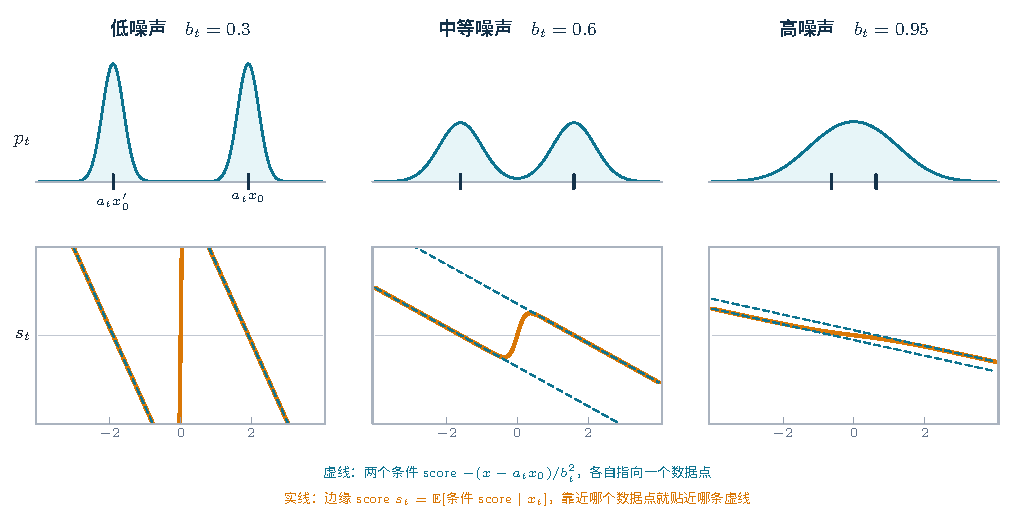
\includegraphics[width=\textwidth]{score_noise_levels.pdf}
\caption{两个数据点在三个噪声水平下的密度与 score。上排是带噪边缘密度 \(p_t\)，竖线标出两个高斯中心 \(a_tx_0,a_tx_0'\)。下排虚线是两个条件 score \(c_t=-(x-a_tx_0)/b_t^2\)，实线是边缘 score \(s_t=\E[c_t\mid x_t]\)，三列纵轴比例相同。低噪声时条件 score 很陡，边缘 score 在两峰之间几乎跳变；中等噪声时过渡变缓；高噪声时两条条件 score 接近重合，边缘 score 几乎是一条直线。去噪网络回归的标签是虚线，学到的是实线。}
\label{fig:score-noise-levels}
\end{figure}

同一网络还可以改为预测干净样本 \(\hat x_0\) 或旋转坐标 \(v=a_t\epsilon-b_tx_0\)，三者满足
\begin{equation}
 \hat x_0=\frac{x_t-b_t\epsilon_\theta}{a_t},\qquad
 \hat x_0=a_tx_t-b_t\hat v,\qquad
 \hat\epsilon=b_tx_t+a_t\hat v.
\end{equation}
这里利用了 \(a_t^2+b_t^2=1\)；这些转换在相应分母非零的时间区间成立。\(v\) 在这里是信号与噪声的旋转坐标；后文 Flow Matching 使用另一个时间变量与速度记号。不同输出参数化若要对应同一个训练目标，还必须相应调整损失权重。

\subsection{从随机扩散到概率流}

为了统一描述加噪步长和采样器，先把离散时间细化到连续时间。随机微分方程（Stochastic Differential Equation，SDE）同时描述确定性漂移和布朗噪声：
\begin{equation}
 dx=f(x,t)\,dt+g(t)\,dW_t.
 \label{eq:forward-sde}
\end{equation}
其中 \(f\) 是确定性的漂移速度，\(g\) 是噪声幅度。可以把 \(W_t\) 理解为连续时间的随机游走。具体地，它是与 \(x\) 同维的标准布朗运动：在长度为 \(\Delta t>0\) 的时间段内，增量 \(\Delta W_t=W_{t+\Delta t}-W_t\sim\mathcal N(0,\Delta t\,I)\)，不重叠时间段的增量相互独立。实际按小步长 \(\Delta t\) 模拟时，上式对应
\begin{equation}
 x_{t+\Delta t}\approx x_t+f(x_t,t)\Delta t+g(t)\sqrt{\Delta t}\,z,
 \qquad z\sim\mathcal N(0,I).
 \label{eq:forward-sde-step}
\end{equation}
每一步重新抽取 \(z\)。例如令 DDPM 的单步噪声方差为 \(\beta(t)\,dt\)，并用 \(\sqrt{1-\beta(t)dt}\approx1-\tfrac12\beta(t)dt\)，得到 \(f(x,t)=-\tfrac12\beta(t)x\)、\(g(t)=\sqrt{\beta(t)}\)。这说明离散 DDPM 的加噪链如何进入连续时间描述。

正向 SDE 从数据分布 \(p_0\) 走向易采样的 \(p_T\)。当 \(g\) 仅依赖时间、密度与系数足够光滑时，反向过程为
\begin{equation}
 dx=[f(x,t)-g(t)^2s_t(x)]\,dt+g(t)\,d\bar W_t,\qquad t:T\to0.
 \label{eq:reverse-sde}
\end{equation}
\(\bar W_t\) 表示沿反向时间抽取的布朗噪声。式中 \(t\) 从 \(T\) 减小到 0，因而 \(dt<0\)，噪声增量的协方差为 \(I|dt|\)。反向漂移中的 score 项可以用一个小时间步看清楚：令 \(h>0\)，已知当前状态 \(x_t=y\)，求更早的 \(x_{t-h}\)。正向短步转移近似为均值 \(x+f(x,t)h\)、协方差 \(g(t)^2hI\) 的高斯核；贝叶斯公式给出
\begin{equation}
 q(x_{t-h}=x\mid x_t=y)\propto p_{t-h}(x)\,q(x_t=y\mid x_{t-h}=x).
 \label{eq:reverse-bayes-step}
\end{equation}
在 \(x\) 接近 \(y\) 处，把 \(\log p_{t-h}(x)\) 作一阶展开，梯度在 \(h\to0\) 时趋于 \(s_t(y)\)。令 \(\delta=x-y\)，将展开式与高斯核相乘并配方，得到
\begin{equation}
\begin{aligned}
 \log q(x_{t-h}=x\mid x_t=y)
 &\simeq C-\frac{\|\delta+f(y,t)h\|^2}{2g(t)^2h}+s_t(y)^\mathsf T\delta\\
 &=C'-\frac{\|\delta-[-f(y,t)+g(t)^2s_t(y)]h\|^2}{2g(t)^2h},
\end{aligned}
 \label{eq:reverse-complete-square}
\end{equation}
其中 \(C,C'\) 不依赖 \(x\)。因此反向一步近似为高斯分布，其均值与协方差是
\begin{equation}
 x_{t-h}\mid x_t=y\ \approx\ \mathcal N\!\left(y+[-f(y,t)+g(t)^2s_t(y)]h,\ g(t)^2hI\right).
 \label{eq:reverse-step-kernel}
\end{equation}
这正是式 \eqref{eq:reverse-sde} 在 \(dt=-h\) 时的一步更新。直观上，在所有可能演化到 \(y\) 的起点中，原本密度较高的起点更可能被选中；\(s_t=\nabla\log p_t\) 给出这项概率修正的方向。

若希望从同一个初始噪声确定性地生成样本，可以寻找具有相同边缘密度的常微分方程。前面已经从噪声网络得到所需的 score；现在把概率密度的扩散写成由速度场驱动的输运。式 \eqref{eq:forward-sde} 对应的福克--普朗克方程是
\begin{align}
 \partial_t p_t
 &=-\nabla\cdot(f p_t)+\tfrac12g(t)^2\Delta p_t\\
 &=-\nabla\cdot\left[\left(f-\tfrac12g(t)^2s_t\right)p_t\right],
 \label{eq:fokker-planck-flow}
\end{align}
第二行使用 \(\nabla p_t=p_ts_t\)。而 ODE \(dx/dt=u_t(x)\) 的密度满足连续性方程 \(\partial_tp_t=-\nabla\cdot(u_tp_t)\)。逐项比较即得概率流 ODE：
\begin{equation}
 \frac{dx}{dt}=u_t(x):=f(x,t)-\tfrac12g(t)^2s_t(x).
 \label{eq:probability-flow}
\end{equation}
因此它与正向 SDE 描述同一族 \(p_t\)；将其从 \(T\) 积分回 0，可用于生成。上面的贝叶斯反向转移也依次经过这族 \(p_t\)。反向 SDE 与反向积分的概率流 ODE 由此具有相同的时间边缘分布，但单条采样轨迹不同。

\Needspace{6\baselineskip}
\textbf{反向扩散与 Langevin：像在哪，不同在哪。}第 \ref{sec:ebm-mcmc} 节的 Langevin 迭代也是“沿 score 走一步，再加高斯噪声”。把 \(-\nabla_xE_\theta\) 记作 score \(s\)，式 \eqref{eq:langevin-step} 写成
\begin{equation}
 x\leftarrow x+\tfrac{\eta}{2}s(x)+\sqrt\eta\,\xi.
\end{equation}
把 \(\epsilon_\theta=-b_ts_t\) 代入式 \eqref{eq:ddpm-reverse-mean}，DDPM 的反向一步变成
\begin{equation}
 x_{t-1}=\frac{x_t+\beta_ts_t(x_t)}{\sqrt{\alpha_t}}+\sigma_tz.
\end{equation}
两者形式相近，却不是同一种算法。取 \(\sigma_t^2\approx\beta_t\)，并只保留 \(\beta_t\) 的一阶项（\(1/\sqrt{\alpha_t}\approx1+\beta_t/2\)），这一步可以拆成两半：
\begin{equation}
 x_{t-1}\approx x_t
 +\underbrace{\tfrac12\beta_t\bigl[x_t+s_t(x_t)\bigr]}_{\text{概率流 ODE 的一步}}
 +\underbrace{\tfrac12\beta_ts_t(x_t)+\sqrt{\beta_t}\,z}_{\eta=\beta_t\text{ 的 Langevin 一步}}.
 \label{eq:ddpm-langevin-split}
\end{equation}
第一项正是式 \eqref{eq:probability-flow} 在 \(f=-\tfrac12\beta x\)、\(g^2=\beta\) 时沿反向时间走的一步，它把分布从 \(p_t\) 推到 \(p_{t-1}\)。第二项是以 \(p_t\) 为目标的 Langevin 一步；按第 \ref{sec:ebm-mcmc} 节的 Fokker--Planck 验证，它让 \(p_t\) 保持不变，只在同一分布内部重新搅动样本。连续时间里，同样的拆分就是反向 SDE 漂移的恒等式
\begin{equation}
 f-g^2s_t=\bigl(f-\tfrac12g^2s_t\bigr)-\tfrac12g^2s_t,
\end{equation}
前一部分是概率流速度，后一部分与噪声 \(g\,d\bar W_t\) 合起来是一段时长为 \(g^2|dt|\) 的 Langevin 动力学。因此，DDPM 的每一步确实含有半步 Langevin，但另一半是 Langevin 没有的输运；整条采样链并不是在某个固定分布上跑 MCMC。表 \ref{tab:langevin-vs-diffusion} 对照了两者。

\begin{table}[H]
\centering\small
\begin{tabularx}{\textwidth}{>{\bfseries}p{20mm} X X}
\toprule
 & Langevin（第 \ref{sec:ebm-mcmc} 节） & DDPM 反向一步\\
\midrule
目标分布 & 一个固定的 \(p\) & 一串分布 \(p_T\to p_{T-1}\to\cdots\to p_0\)\\
用到的 score & 每步相同的 \(\nabla\log p\) & 每步换成当前噪声水平的 \(s_t\)\\
单步的作用 & 保持 \(p\) 不变，样本在 \(p\) 内移动 & 输运半步把 \(p_t\) 变成 \(p_{t-1}\)，Langevin 半步只在 \(p_t\) 内搅动\\
步数 & 要等链混合，事先难以确定 & 由所选时间点固定，走完即得样本\\
多峰分布 & 跨越峰间低密度区可能极慢 & 高噪声时各峰已连成一片，样本随噪声降低逐渐分到各峰\\
误差来源 & 有限步长偏差与未混合 & score 估计误差与时间离散误差\\
\bottomrule
\end{tabularx}
\caption{Langevin 采样与 DDPM 反向采样的对照。}
\label{tab:langevin-vs-diffusion}
\end{table}

多峰一行是两者最实质的差别。Langevin 要在固定的多峰分布里从一个峰走到另一个峰，必须穿过低密度区，等待时间随势垒高度指数增长。反向扩散从近似单峰的 \(p_T\) 出发，此时各峰尚未分开；随着噪声逐级降低，样本由输运项逐渐分配到不同的峰，各峰所得的样本比例由这条分布序列决定，而不靠样本自己越过势垒。

这个拆分也把几种采样器放到同一张图里。只保留输运项，就是确定性的概率流 ODE 采样器；下一小节的 DDIM 可以看作它的一种离散化。只保留 Langevin 项，在每个噪声水平多走若干步、再逐级降低噪声，就是早期 score 模型使用的退火 Langevin 采样~\cite{song2020ncsn}。两项各走一步，就是 DDPM 的反向一步。Song 等人的预测--校正采样器把两部分显式分开：先用反向 SDE 或 ODE 的数值步预测下一噪声水平的样本，再在该水平上做若干步 Langevin 校正~\cite{song2021score}。校正步不改变目标边缘分布，可以减轻数值积分和 score 误差造成的偏离，代价是更多的网络调用。

接下来讨论去噪扩散隐式模型（Denoising Diffusion Implicit Model，DDIM）怎样复用已训练的噪声网络做确定性跳步采样。

\subsection{DDIM：复用噪声网络，改变采样步骤}

先回到 DDPM 的生成程序：在 \(t=T,T-1,\ldots,1\) 的每个时间点调用一次 \(\epsilon_\theta(x_t,t)\)，用式 \eqref{eq:ddpm-reverse-mean} 算当前一步的反向高斯均值，再按式 \eqref{eq:ddpm-sampling-step} 抽样得到 \(x_{t-1}\)。它沿相邻时间点逐步更新，通常要调用网络约 \(T\) 次。要减少调用次数，就需要能直接从当前 \(t\) 更新到选定的更早时间 \(s<t\)。

DDIM 沿用 DDPM 训练时的 \(q(x_t\mid x_0)\)、噪声损失和网络 \(\epsilon_\theta\)，改变生成时连接不同噪声水平的方式~\cite{song2021ddim}。这里先看确定性版本。在当前 \(x_t\) 上调用一次网络，得到噪声预测，并按 \(x_t=a_t\hat x_0+b_t\epsilon_\theta(x_t,t)\) 估计干净图片 \(\hat x_0\)。接着用更早时间 \(s\) 的系数把这两个成分重新组合：
\begin{equation}
 \hat x_0=\frac{x_t-b_t\epsilon_\theta(x_t,t)}{a_t},\qquad
 x_s=a_s\hat x_0+b_s\epsilon_\theta(x_t,t),\quad s<t.
 \label{eq:ddim-update}
\end{equation}
这一更新在一步内从 \(t\) 到达 \(s\)，并沿用当前网络对图像内容与噪声方向的预测。相比之下，DDPM 在每个 \(t\) 只构造到 \(t-1\) 的高斯转移，在中间步另抽一份 \(z\)。确定性 DDIM 的式 \eqref{eq:ddim-update} 在给定初始 \(x_T\) 后不再抽新噪声；两种生成程序使用的是同一套已训练的网络参数。除跳步路径外，噪声水平、网络预条件和数值求解器也会影响采样质量与成本，Karras 等对这些设计做了系统比较~\cite{karras2022edm}。

实际采样时先选一列时间 \(T=t_K>t_{K-1}>\cdots>t_0=0\)，并取 \(a_0=1,b_0=0\)。从 \(x_T\sim\mathcal N(0,I)\) 开始，对每个 \(k=K,\ldots,1\) 令 \(t=t_k,s=t_{k-1}\)，执行一次式 \eqref{eq:ddim-update}。例如原训练调度有 \(T=1000\) 个时间点，生成时只选 \(K=50\) 个更新，就调用网络约 50 次。训练目标和噪声预测不变，改变的是生成时间点与从一个时间点到下一个时间点的更新公式。下一小节介绍常用的 U 形网络（U-Net）与扩散 Transformer（Diffusion Transformer，DiT）。

\subsection{噪声预测网络：U-Net 与 DiT}

前面预测噪声的网络 \(\epsilon_\theta(x_t,t,c)\) 通常采用 U-Net 或 DiT~\cite{peebles2023dit}。扩散模型中的 U-Net 以卷积神经网络（Convolutional Neural Network，CNN）为图像主干：每一级用卷积残差块提取特征，再通过步幅为 2 的卷积把特征图的高和宽减半，并通常增加通道数；恢复路径用插值加卷积或转置卷积把高和宽加倍，把编码路径中相同分辨率的特征通过跳跃连接送来，再用卷积残差块融合。CNN 的下采样扩大感受野，跳跃连接保留细节；一些层还加入自注意力以交换较远位置的信息。DiT 则把带噪图像或潜变量切成 patch 序列，由 Transformer 在 patch 之间交换信息，再投影回噪声预测。

\Needspace{3\baselineskip}
图像扩散也可以先用前述 VAE 式自编码器把图片压缩为连续潜变量，在潜空间逐步去噪，再由解码器还原图片；这减少了去噪网络处理的空间尺寸~\cite{rombach2022ldm}。

网络接收当前时间 \(t\)，\(T\) 决定噪声调度的总步数。一种常见实现先用多种频率的正弦、余弦函数把整数 \(t\) 映射为向量 \(u_t\)，再用一个小型 MLP 计算时间嵌入 \(e_t=\operatorname{MLP}(u_t)\)；图像特征仍由上面的卷积主干处理。U-Net 在各残差块中把 \(e_t\) 投影到特征通道，例如执行 \(h\leftarrow h+W_\ell e_t\)；DiT 可用 \(e_t\) 调节块内自适应归一化的缩放、平移和残差门控。时间输入也可改用对应噪声幅度或对数信噪比。文本等条件 \(c\) 可通过交叉注意力注入，即用当前图像表示查询条件表示。图 \ref{fig:diffusion-denoiser} 把潜空间扩散的流程，以及两种网络中时间与条件的注入位置画在一起。

\begin{figure}[H]
\centering
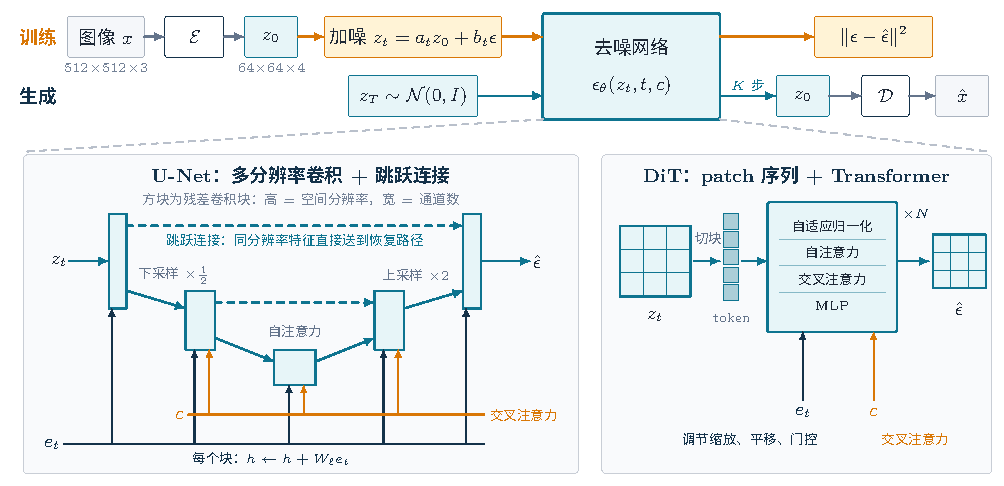
\includegraphics[width=\textwidth]{diffusion_denoiser_arch.pdf}
\caption{潜空间扩散与两种去噪网络。上方：训练时编码器 \(\mathcal E\) 把图像压成潜变量 \(z_0\)，加噪后由网络预测噪声；生成时从 \(z_T\) 出发调用同一网络 \(K\) 步，再由解码器 \(\mathcal D\) 还原图像。左下：U-Net 沿编码路径降低分辨率、增加通道，恢复路径经跳跃连接取回同分辨率特征；时间嵌入 \(e_t\) 加到每个残差块，条件 \(c\) 经交叉注意力进入较低分辨率的块。右下：DiT 把 \(z_t\) 切成 patch token，经 \(N\) 个 Transformer 块后还原为噪声预测；\(e_t\) 调节自适应归一化，\(c\) 经交叉注意力注入。}
\label{fig:diffusion-denoiser}
\end{figure}

当生成还受文本等条件 \(c\) 控制时，常用无分类器引导（classifier-free guidance）增强条件作用。训练时随机把一部分样本的条件替换为空条件，使同一网络既能输出 \(\epsilon_{\mathrm{cond}}=\epsilon_\theta(x_t,t,c)\)，也能输出 \(\epsilon_{\mathrm{uncond}}=\epsilon_\theta(x_t,t,\varnothing)\)。生成时各调用一次网络，将两次预测组合为
\begin{equation}
 \epsilon_{\mathrm{guide}}=\epsilon_{\mathrm{uncond}}+w(\epsilon_{\mathrm{cond}}-\epsilon_{\mathrm{uncond}}).
 \label{eq:cfg}
\end{equation}
\(w=1\) 给出条件预测，\(w>1\) 沿条件与无条件预测之差进一步移动。随后把 \(\epsilon_{\mathrm{guide}}\) 代入 DDPM 或 DDIM 的采样更新；引导改变的是网络给出的更新方向，时间点与采样公式仍由所选采样器决定。按这里分别计算两种预测的做法，每个采样时间需要两次网络调用。

\subsection{Flow Matching：直接学习概率路径的速度}

概率流 ODE 已经把 score 转换成了搬运样本的速度。一个自然的下一步是：能否直接规定从噪声到数据的路径，并把速度当作网络的监督目标？Flow Matching 就采用这一方式~\cite{lipman2023flow}。为与扩散的“数据到噪声”时间区分，本小节用 \(r\in[0,1]\) 表示“噪声到数据”的生成时间。

先看一次训练样本怎样构造。\(y\sim p_{\mathrm{data}}\) 是从数据集中取出的一张真实图片，或它在潜空间中的表示；\(z\sim\mathcal N(0,I)\) 是独立抽取、形状与 \(y\) 相同的高斯噪声。再随机抽 \(r\sim\operatorname{Uniform}[0,1]\)，计算 \(x_r=(1-r)z+ry\)：\(r=0\) 时它是噪声 \(z\)，\(r=1\) 时它是数据 \(y\)。对这一对固定端点，沿 \(r\) 求导得到 \(dx_r/dr=y-z\)；它是从噪声走向真实图片时每单位时间的位移，因而可以直接由已知的 \(y,z\) 算作速度标签。网络 \(v_\theta(x_r,r)\) 接收中间状态和时间，输出与 \(x_r\) 形状相同的预测速度；网络主体也可采用前述 U-Net 或 DiT，并把 \(r\) 作为时间嵌入输入。训练目标是
\begin{equation}
 \mathcal L_{\mathrm{velocity}}
 =\E_{y,z,r}\|v_\theta(x_r,r)-(y-z)\|^2.
 \label{eq:flow-matching}
\end{equation}
实际处理一个大小为 \(B\) 的 minibatch 时，对每张真实图片 \(y_i\) 各抽一个 \(z_i,r_i\)，构造 \(x_{r_i}=(1-r_i)z_i+r_i y_i\) 和标签 \(u_i=y_i-z_i\)。把 \((x_{r_i},r_i)\) 输入网络，逐像素或逐潜变量坐标比较预测速度与 \(u_i\)，再对 batch 取平均：
\begin{equation}
 \widehat{\mathcal L}_{\mathrm{velocity}}=\frac1B\sum_{i=1}^{B}
 \|v_\theta(x_{r_i},r_i)-(y_i-z_i)\|^2.
 \label{eq:flow-matching-batch}
\end{equation}
随后对这个损失反向传播，更新网络参数 \(\theta\)。这里的 \(y_i-z_i\) 是\textbf{速度监督标签}；训练中的梯度是损失对参数 \(\theta\) 的梯度，使网络输出靠近这个标签。在固定 \(x_r=x\) 处，许多不同的 \((y,z)\) 可以产生同一个中间状态，均方回归的最优网络输出是这些速度的条件平均 \(v_r(x)=\E[y-z\mid x_r=x]\)。

这解释了训练标签看似矛盾的地方。网络只看到当前位置与时间，同一输入可能对应多个速度；它在总体均方损失下学到的是这些速度的条件重心。不同的 \(x_r\) 有不同的端点后验，得到的平均速度也不同；生成器沿这个随位置与时间变化的速度场运动。

结论与去噪得分匹配相同：回归条件速度标签，学到的就是搬运边缘分布所需的速度场。理由有两层。第一层是损失本身：与推出式 \eqref{eq:denoising-score} 的正交分解完全相同，在平方中插入 \(v_r(x_r)\) 后交叉项为零，于是
\begin{equation}
 \E\|v_\theta(x_r,r)-(y-z)\|^2
 =\E\|v_\theta(x_r,r)-v_r(x_r)\|^2+C,
 \label{eq:cfm-marginal-equivalence}
\end{equation}
其中 \(C=\E\|(y-z)-v_r(x_r)\|^2\) 是给定 \((x_r,r)\) 后剩余的条件方差，与 \(\theta\) 无关。两种损失的梯度处处相同；\(C>0\) 也说明单对端点的速度有无法从 \((x_r,r)\) 推出的随机部分，训练损失不会降到零。第二层是这个平均速度确实搬运整条概率路径。固定一个数据样本 \(y\) 时，直线上的局部速度是 \(u_r(x\mid y)=(y-x)/(1-r)\)，条件密度 \(p_r(x\mid y)\) 满足连续性方程。对所有 \(y\) 的概率流量求平均，得到
\begin{equation}
 p_r(x)v_r(x)
 =\int p_{\mathrm{data}}(y)\,p_r(x\mid y)\,u_r(x\mid y)\,dy,
 \qquad
 \partial_r p_r(x)+\nabla\cdot\bigl(p_r(x)v_r(x)\bigr)=0.
 \label{eq:flow-matching-marginal-flux}
\end{equation}
第一式是各条条件路径在 \(x\) 处的流量叠加；第二式由条件连续性方程对 \(y\) 积分得到。因此按 \(v_r\) 积分生成 ODE 时，样本在每个 \(r\) 的分布都是训练路径的边缘 \(p_r\)，到 \(r=1\) 就是数据分布；单条生成轨迹与训练用的直线不必相同。

直线路径还给出一个具体图像。在 \(r=0\) 时 \(x_r=z\) 与 \(y\) 独立，所以 \(v_0(x)=\E[y]-x\)。当 \(0<r<1\) 时，由 \(x_r=ry+(1-r)z\) 和高斯噪声得到
\begin{equation}
 p(y\mid x_r=x)\ \propto\ p_{\mathrm{data}}(y)
 \exp\!\left[-\frac{\|x-ry\|^2}{2(1-r)^2}\right].
 \label{eq:flow-matching-endpoint-posterior}
\end{equation}
随着 \(r\) 增大，当前位置对可能的目标数据提供越来越强的约束：不同位置偏向不同的数据区域，速度场便把不同噪声起点引向不同的方向。每一步都会在新的位置重新计算速度，因此这条生成轨迹可以弯曲。

生成新图片时，重新抽一张噪声 \(x^{(0)}=z_{\mathrm{new}}\sim\mathcal N(0,I)\)，选 \(N\) 个时间步 \(r_k=k/N\)、\(\Delta r=1/N\)。每一步用当前状态与时间调用速度网络，再沿预测方向前进一步；最简单的欧拉更新为
\begin{equation}
 x^{(k+1)}=x^{(k)}+\Delta r\,v_\theta(x^{(k)},r_k),
 \qquad k=0,\ldots,N-1.
 \label{eq:flow-matching-euler}
\end{equation}
最后的 \(x^{(N)}\) 就是生成图片。推断时网络只使用当前 \(x^{(k)}\) 与 \(r_k\) 来给出下一步速度；训练所用的真实图片 \(y_i\) 只用于构造监督标签。每对训练端点定义一条直线，条件平均后的速度场可以产生弯曲的生成轨迹。

它与扩散模型的数学关系可以在一般高斯路径上看清。令 \(x_r=a(r)y+b(r)z\)，以 \(p_r\) 表示边缘密度、\(s_r=\nabla\log p_r\)，并在 \(a,b>0\) 的内部时间区间计算。式 \eqref{eq:marginal-score-identity} 给出
\begin{equation}
 \E[z\mid x_r=x]=-b(r)s_r(x),\qquad
 \E[y\mid x_r=x]=\frac{x+b(r)^2s_r(x)}{a(r)}.
\end{equation}
条件速度是 \(\dot a\,y+\dot b\,z\)，点表示对 \(r\) 求导。取条件均值并代入上式得到
\begin{equation}
 v_r(x)=\frac{\dot a}{a}x+
 \left(\frac{\dot a}{a}b^2-b\dot b\right)s_r(x).
 \label{eq:flow-score-bridge}
\end{equation}
式 \eqref{eq:flow-score-bridge} 可以代入两种具体路径。先代入本小节训练用的直线路径 \(a(r)=r,b(r)=1-r\)，此时 \(\dot a=1,\dot b=-1\)，得到
\begin{equation}
 v_r(x)=\E[y-z\mid x_r=x]
 =\frac{x}{r}+\frac{1-r}{r}s_r(x),\qquad 0<r<1.
 \label{eq:straight-flow-score}
\end{equation}
左边正是式 \eqref{eq:flow-matching} 的均方回归在固定 \(x_r=x\) 时学到的速度；右边把同一速度写成了边缘密度的 score。

再代入 DDPM 高斯加噪的连续时间版本。若离散单步方差按 \(\beta_s\approx\beta(t_s)\Delta t\) 缩小，则乘积 \(\bar\alpha_t=\prod_s(1-\beta_s)\) 趋于 \(\bar\alpha(t)=\exp[-\int_0^t\beta(u)\,du]\)。于是正向路径 \(x_t=a(t)y+b(t)z\) 的两个系数为 \(a(t)=\sqrt{\bar\alpha(t)}\)、\(b(t)=\sqrt{1-\bar\alpha(t)}\)。它们满足
\begin{equation}
 \frac{\dot a(t)}{a(t)}=-\frac{\beta(t)}2,\qquad
 b(t)\dot b(t)=\frac{\beta(t)}2a(t)^2,\qquad a(t)^2+b(t)^2=1.
 \label{eq:vp-path-derivatives}
\end{equation}
逐项代入式 \eqref{eq:flow-score-bridge}，便得到
\begin{equation}
\begin{aligned}
 v_t(x)
 &=-\frac{\beta(t)}2x-\frac{\beta(t)}2[b(t)^2+a(t)^2]s_t(x)\\
 &=-\frac{\beta(t)}2x-\frac{\beta(t)}2s_t(x)
 =f(x,t)-\frac12g(t)^2s_t(x),
\end{aligned}
 \label{eq:vp-flow-from-bridge}
\end{equation}
其中 \(f(x,t)=-\beta(t)x/2\)、\(g(t)^2=\beta(t)\)，正是前面 DDPM 连续化得到的漂移和噪声强度。因此同一个一般公式既给出直线 Flow Matching 的最优速度，也给出扩散路径的式 \eqref{eq:probability-flow}。如果 Flow Matching 训练时也选用后一组 \(a(t),b(t)\)，它学到的就是这条扩散路径的概率流速度；本小节先前演示的直线路径则给出另一条速度场。扩散路径的公式按正向时间 \(t\) 表示数据到噪声的速度；生成时从 \(T\) 积分回 0，或改用 \(r=1-t/T\) 并把速度乘以 \(dt/dr=-T\)。这里得到的是确定性的概率流速度，DDPM 的随机反向高斯更新由式 \eqref{eq:ddpm-sampling-step} 给出。

现在可以把第 \ref{sec:cnf} 节的 CNF 与本小节接起来：两者在生成时都从基分布沿 \(dx_r/dr=v_\theta(x_r,r)\) 积分，密度都遵循式 \eqref{eq:cnf-density}。CNF 指这种连续时间的可逆概率变换；Flow Matching 给出学习其速度场的一种监督方法。传统似然训练对每个数据样本求解 ODE 和散度积分，再优化 \(-\log p_1(x)\)；Flow Matching 则先指定具有解析采样公式的条件路径，随机取一个时间和一对端点，直接构造 \(x_r\) 与条件速度标签，按式 \eqref{eq:flow-matching} 回归，训练时不要求解生成 ODE。生成时仍按式 \eqref{eq:flow-matching-euler} 或更精确的求解器积分。若任务需要评价样本密度，也可对训练好的速度场反向积分并累积散度，由 CNF 公式得到 \(\log p_\theta(x)\) 的数值结果。

\begin{table}[H]
\centering\small
\begin{tabularx}{\textwidth}{>{\bfseries}p{28mm} X X}
\toprule
训练方式 & 参数更新时的计算 & 生成与密度评价\\
\midrule
CNF 的似然训练 & 从数据反向求解状态与散度，优化负对数似然 & 积分速度 ODE 生成；积分散度评价密度\\
Flow Matching & 解析构造随机时刻的状态和条件速度，做均方回归 & 积分同类速度 ODE 生成；需要密度时也积分散度\\
\bottomrule
\end{tabularx}
\caption{CNF 的两种训练路径共享连续时间的生成与密度公式。}
\label{tab:cnf-flow-matching}
\end{table}

\begin{figure}[H]
\centering
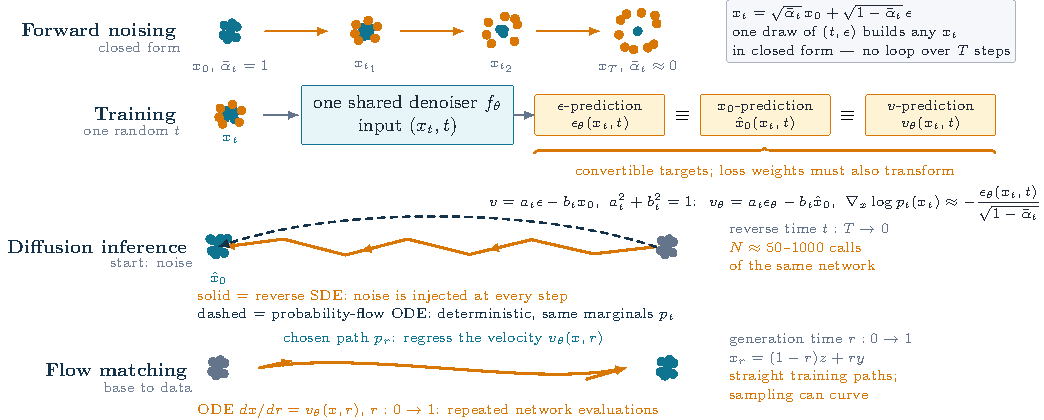
\includegraphics[width=\textwidth]{diffusion_score_flow_paths.pdf}
\caption{训练与生成的四条轨道。正向加噪可直接构造任意时间的训练样本；噪声、干净样本和旋转坐标是可转换的预测对象。扩散采样反向积分 SDE 或概率流 ODE；Flow Matching 用生成时间 \(r\) 直接回归速度并积分。两者通常都需要多次网络调用，相同边缘分布不要求单条轨迹相同。}
\label{fig:diffusion-score}
\end{figure}

\begin{table}[H]
\centering\small
\begin{tabularx}{\textwidth}{>{\bfseries}p{28mm} X X X}
\toprule
方法 & 训练目标 & 生成更新 & 相对 DDPM 的变化\\
\midrule
DDPM & 噪声回归 & 相邻时间的反向高斯转移 & 基线：逐步更新并在中间步抽新噪声\\
连续时间 score & 带噪分布的 score 回归 & 反向 SDE 或概率流 ODE & 用连续时间方向场描述生成\\
确定性 DDIM & 复用 DDPM 的噪声网络 & 从 \(t\) 直接到选定的 \(s<t\) & 由 \(\hat x_0\) 和噪声预测重组，减少网络调用\\
Flow Matching & 所选路径的速度回归 & 从基分布积分速度 ODE & 直接学习速度场，可选择不同概率路径\\
掩码离散扩散 & 被掩码 token 的类别预测及时间加权 & 从全掩码序列逐步恢复 token & 用类别转移代替高斯噪声，可在一轮更新多个位置\\
\bottomrule
\end{tabularx}
\caption{扩散与速度场模型各自改变的数学对象。}
\label{tab:diffusion-score-variants}
\end{table}

\section{模型家族的选择原则}

模型选择的差别可以直接落到任务约束上。下表按模型汇总四件事：它适合什么任务、训练时从哪里得到梯度、推理时沿哪条路径采样、以及代价落在哪里。

\begin{table}[ht]
\centering\scriptsize
\begin{tabularx}{\textwidth}{>{\bfseries}p{19mm} p{26mm} X X X}
\toprule
模型 & 适合的任务约束 & 训练目标与随机性 & 推理路径 & 代价与失效模式\\
\midrule
自回归 & 离散序列、逐步条件控制、需要 token likelihood
& 真实序列 + causal mask，最小化 NLL；训练不需要从模型采样，softmax、注意力和 FFN 全部可微
& 从 BOS 逐 token ancestral sampling，每步读取历史缓存；输入可并行，生成串行
& 串行延迟随输出长度增长；exposure bias；长上下文记忆成本高\\

VAE & 连续数据、需要低维表示和快速重构
& encoder 给 \(q_\phi(z\mid x)\)，decoder 给 \(p_\theta(x\mid z)\)；重参数化，KL 对角高斯时解析
& \(z\sim p(z)\) 后一次 decoder 得到条件分布，再采样 \(x\)；推断时运行 encoder
& 只优化下界；重构偏平滑；强 decoder 会忽略 latent，出现 posterior collapse\\

Flow / RealNVP & 连续数据、需要精确 likelihood、可逆编码或重要性加权
& 变量替换，log-det 解析；训练不需要随机 latent
& \(z\sim p_Z\) 后按逆层一次得到 \(x\)，每层都要反变换
& 可逆结构限制表达；高维 patch、scale 稳定性和多层逆变换带来成本\\

GAN & 单次前向延迟极低、允许隐式分布
& 判别器 BCE 与生成器 minimax 或 non-saturating loss 交替；给定 \(z\)，生成器到判别器的路径可微
& \(z\) 一次过 \(G\)，部署吞吐高
& 无 likelihood；博弈非凸、mode collapse、Nash 均衡难达到\\

Diffusion/\allowbreak Score & 图像或连续场、峰值质量优先、允许多步采样
& 随机抽 \(t,\epsilon\) 构造 \(x_t\)，回归 \(\epsilon\)、\(x_0\)、\(v\) 或 score；普通反传
& 从 \(x_T\) 反复求解 reverse SDE/ODE，\(N_{\mathrm{step}}\) 次网络调用
& 采样成本乘步数；solver、噪声调度和 guidance 改变样本分布\\

EBM & 只知道能量、守恒量或未归一化目标密度
& 正相位降低数据能量，负相位从 \(p_\theta\) 链采样；MCMC 噪声不能直接沿长链反传
& Langevin/MCMC 多步迭代，单步网络便宜但混合可能极慢
& 配分函数和负相位难算；局部链不能代表全局模式\\
\bottomrule
\end{tabularx}
\caption{按模型对照任务约束、训练随机性与梯度路径、推理路径和主要代价。}
\label{tab:model-selection-explicit}
\end{table}

如果任务是“给定前缀继续生成”，自回归模型的优势来自条件分解本身；如果任务是“从噪声一次得到连续样本”，GAN 或 VAE 的单次 decoder 路径更短，但它们对高频细节和分布覆盖的取舍不同。如果必须报告每个样本的 likelihood，GAN 无法给出，VAE 给出 ELBO，可逆流则用变量变换评价密度：RealNVP 显式累加 log-determinant，CNF 数值积分散度。若目标侧重图像感知质量，连续扩散通常以更多采样步换取更稳的多峰覆盖；离散文本也可用掩码扩散逐轮填充，速度与质量需要按具体任务评估。若目标密度由已知能量给出，EBM 的优势是目标写法自然，难点则从表达转移到 MCMC 的负相位和混合。

\section{六类模型的一次实际训练循环}

一次 minibatch 的操作顺序把公式落成可执行计算：从哪一个随机变量、哪一条网络路径和哪一种概率对象算出来。

\subsection{自回归 Transformer}

给定 batch 中的真实序列 \(x_{1:T}\)，先把输入右移一位，形成 \(\langle\mathrm{BOS}\rangle,x_1,\ldots,x_{T-1}\)，经过 embedding、位置编码和 \(L\) 个 decoder block，得到每个位置的 logits \(l_t\)。对真实标签 \(x_t\) 计算
\begin{equation}
\mathcal L_{\mathrm{autoregressive}}=-\frac1T\sum_{t=1}^{T}
\log\operatorname{softmax}(l_t)_{x_t}.
\end{equation}
causal mask 使一次前向同时产生全部 \(T\) 个位置；反向传播更新词向量嵌入、注意力、前馈网络和输出投影。训练时通常只使用 dropout、数据顺序或数据增强中的随机性，不需要从模型的 \(p_\theta\) 采样。推理从 BOS 开始，算出下一个 token 的分布后抽样并追加，再重复运行；历史缓存保存旧 token 已计算的表示，避免每一步重算前缀；具体保存哪些张量将在下一章说明。

\subsection{VAE}

对一个 minibatch 的每个观测 \(x\)，encoder 产生 \(\mu_\phi(x),\log\sigma_\phi^2(x)\)，从独立高斯 \(\epsilon\) 构造 \(z^{(k)}=\mu_\phi(x)+\sigma_\phi(x)\odot\epsilon^{(k)}\)，decoder 产生 \(p_\theta(x\mid z^{(k)})\) 的参数。按式~\eqref{eq:vae-mc-loss} 估计每个 \(x\) 的负 ELBO，再对 minibatch 取平均；标准 VAE 的 KL 系数为 \(1\)，另设系数 \(\beta\neq1\) 时是加权变体。观测 \(x\) 在 decoder 分布下的负对数概率沿 decoder 和重参数化路径更新 \(\theta,\phi\)，KL 项沿 encoder 的 \(\mu,\log\sigma^2\) 更新 \(\phi\)。二值数据的 Bernoulli 选择给出逐位交叉熵；连续数据的固定方差高斯选择给出带尺度的均方误差。生成阶段不需要 encoder：先采样 \(z\sim p(z)\)，再从 decoder 给出的条件分布采样 \(x\)。

\subsection{RealNVP Flow}

给定数据 \(x\)，依次运行每层 coupling transform 得 \(z=f_\theta(x)\)，计算 base log-density 与每层 scale 的和：
\begin{equation}
\mathcal L_{\mathrm{Flow}}
=-\log p_Z(z)-\sum_{\ell}\sum_j s_{\ell,j}(x_{a,\ell}).
\end{equation}
由于正向变换和 log-determinant 都是确定可微的，梯度直接更新每层产生 \(s,t\) 的网络；训练中没有从 \(z\) 采样。部署时从 \(z\sim p_Z\) 开始，按逆序计算 \(x_b=(z_b-t(z_a))e^{-s(z_a)}\)，无需迭代求解。若还要做 importance sampling，可用 exact \(p_X(x)\) 对样本重加权；这正是 Flow 相对 GAN/VAE 的概率优势。

\subsection{生成对抗网络}

一次训练循环包含判别器更新与生成器更新，两步分别使用各自的损失。

每个 discriminator step 取真实 batch \(x\sim p_{\mathrm{data}}\) 和噪声 batch \(z\sim p_Z\)，构造 \(x_g=G_\theta(z)\)，最小化
\begin{equation}
\mathcal L_D=-\E_x\log D_\phi(x)-\E_z\log(1-D_\phi(x_g)).
\end{equation}
随后冻结 \(D\)，重新取噪声或复用 \(x_g\)，最小化
\(\mathcal L_G=-\E_z\log D_\phi(G_\theta(z))\)。判别器的梯度不能更新生成器，生成器的梯度必须通过 \(D(G(z))\) 回到 \(G\)；因此实现上要在两个 optimizer step 之间切换 requires-grad。推理时只保留 \(G\)，每个噪声一次前向得到一个样本；训练的不稳定来自两个网络的相对速度和分布支撑，与采样链无关。

\subsection{Diffusion / Score}

每个训练样本只随机抽一个时间 \(t\) 和一个噪声 \(\epsilon\)，通过
\begin{equation}
x_t=a_tx_0+b_t\epsilon,\qquad a_t=\sqrt{\bar\alpha_t},\quad b_t=\sqrt{1-\bar\alpha_t},
\end{equation}
构造网络输入，计算 \(\|\epsilon-\epsilon_\theta(x_t,t,c)\|^2\)，再标准反向传播。随机噪声不需要对 \(\epsilon\) 求梯度；它只是把同一个 \(x_0\) 变成不同噪声层级的训练实例。推理从 \(x_T\sim\mathcal N(0,I)\) 开始，重复调用同一 denoiser 并使用离散 reverse update、SDE solver 或 probability-flow ODE solver；一次样本需要 \(N_{\mathrm{step}}\) 次网络前向，因此采样成本与步数直接相乘。

\subsection{EBM}

每次更新先用真实数据计算 positive phase，再从当前能量模型的 MCMC 链得到 negative samples，使用
\begin{equation}
\widehat{\nabla_\theta\mathcal L}
=\frac1B\sum_i\nabla_\theta E_\theta(x_i^{+})
-\frac1B\sum_i\nabla_\theta E_\theta(x_i^{-}).
\end{equation}
短链得到的 \(x_i^{-}\) 与真实独立样本有偏差，所以参数更新和采样链互相影响。一个具体的 persistent chain 循环是：初始化并保存 \(M\) 个链状态；每个 minibatch 到来时，从这些旧状态各走 \(k\) 步 Gibbs、Metropolis--Hastings 或 Langevin 更新；用终点估计 negative phase；完成一次参数更新；最后把终点写回状态池，供下一 minibatch 继续。它省掉了每轮从随机初值重新 burn-in，却引入两类偏差：有限 \(k\) 使样本相关，参数在链尚未平衡时已经变化；若能量面有分离很远的模式，链还可能长期困在某一模式。实务中应监控多链能量、模式占比、自相关时间和跨模式跃迁，与训练 loss 一起看。推理阶段也运行同样的链，模型的表达和目标密度写法很灵活，代价集中在负相位和混合。

\begin{table}[H]
\centering\small
\begin{tabularx}{\textwidth}{>{\bfseries}p{26mm} X X X}
\toprule
模型 & 每步抽什么随机量 & 梯度从哪里来 & 推理调用几次网络\\
\midrule
自回归 & 数据顺序、dropout & 词表交叉熵，全部可微 & 每个新 token 一次，读取历史缓存\\
VAE & $\epsilon\sim\mathcal N(0,I)$ & 重参数化路径，KL 解析式 & 一次 decoder\\
RealNVP & 训练时无；生成时 $z\sim p_Z$ & 变量替换，正向与逆变换都可微 & 每层一次逆变换\\
GAN & $z\sim p_Z$ & 经判别器 $D(G(z))$ 回传 & 一次生成器\\
Diffusion & $t,\epsilon$ & 噪声回归，普通反向传播 & $N_{\mathrm{step}}$ 次 denoiser\\
EBM & MCMC 链的状态 & 正负相位，链本身不反传 & 多步 MCMC\\
\bottomrule
\end{tabularx}
\caption{六个训练循环只差三处：每步抽什么随机量、梯度沿哪条路径回传、推理要调用几次网络。}
\label{tab:six-loops}
\end{table}

\chapter{Transformer：整体结构、训练目标与内部组件}
\label{chap:transformer}

\begin{keybox}[先看整台模型，再看一层内部]
Transformer 把一组 token 向量变成一组包含上下文信息的向量。注意力负责位置之间的信息交换，前馈网络负责位置内部的特征变换，残差连接与归一化让这些层可以反复堆叠。网络最后接什么输出头、每个位置允许读取什么信息，以及用什么损失训练，共同决定它是文本表示模型、条件生成模型还是自回归语言模型。
\end{keybox}

在展开具体结构之前，先回答一个容易被跳过的问题：离散文本的生成，为什么最后是自回归占了主流？这里没有一条定理保证它，只是几件事叠在一起的结果。

第一，链式法则给出的是精确、逐项归一化的似然。每个位置只是一个 \(|\mathcal V|\) 类分类问题，损失是交叉熵，训练目标没有额外的近似。第二，teacher forcing 让所有位置在一次前向里并行监督，而且每个 token 都贡献一项损失，监督信号密集。第三，序列长度是可变的，生成长度由模型自己决定，不需要为不同长度设计特殊机制。第四，条件化几乎免费：提示词就是前缀，条件生成不需要另外的接口。第五，工程上键值缓存（Key--Value cache，KV cache）把串行解码的重复计算去掉，批处理与推测解码再把固定开销摊薄，串行不再等于不可接受。

离散扩散是主要的替代方案。它需要额外设计吸收态和转移矩阵，多个位置同时去掩码时还要保证联合分布的一致性；连续扩散在图像上的成功不能直接搬过来。它在并行采样和可控性上有优势，但训练目标和采样程序都比自回归复杂。

所以更准确的说法是：自回归在离散序列上的优势，来自“目标简单、监督密集、工程成熟”的叠加。如果硬件形态或算法改变——例如并行采样的收益变得更大，或者离散扩散的训练目标变得更简单——这个格局未必不变。

\section{Transformer 的共同骨架与三种模型结构}

\subsection{共同输入与层内骨架：从 token 到上下文表示}

在自然语言处理中，原始文字先由分词器（tokenizer）按预先确定的规则转换为 token 编号序列 \(x_1,\ldots,x_T\)，每个编号都属于有限词表 \(\mathcal V\)。token 可以是完整单词、字、子词、标点或其他文本片段；词表通常还包含 BOS、EOS 等特殊 token。编号只是类别标签，编号顺序只是词表中的索引，与语义距离无关。词表和切分规则通常在模型训练前确定，它们会影响序列长度 \(T\) 和后续词表矩阵的大小。

分词器本身是一个独立的预处理算法。以字节对编码（Byte-Pair Encoding，BPE）为例：从字符或字节开始，统计语料中相邻符号对的频率，反复把最高频的一对合并成新符号，直到词表达到预定大小；合并规则固定后，训练和推理都使用同一套规则~\cite{sennrich2016bpe,radford2019gpt2}。字节级 BPE 先把文本转成 UTF-8 字节，因此任何字符都能表示：未登录词只会拆成更多的字节 token，词表中不需要未知词标记 UNK（unknown）。

词表大小是一个取舍。词表越大，同样的文本切成越少的 token，序列更短，注意力和 KV cache 的成本随之下降；但输入嵌入和输出 softmax 的参数量、以及稀有 token 的统计量都会增加。中文、日文等多字节文字在字节级词表下通常占更多 token；数字常被拆成单个数字，这对算术有利也有弊；科学文本里的公式、单位和上下标往往没有专门的 token，会被切成不自然的片段。这些切分方式直接影响模型看到什么。

特殊 token 还承担结构标记：BOS、EOS、填充、对话角色等。对话模板把多轮消息拼成一条带标记的序列，训练和推理必须使用同一套模板，否则条件分布会对不上。不同 tokenizer 的 per-token 概率不能直接比较，这一点在评价语言模型时会再次用到。

输入嵌入矩阵 \(E\in\R^{|\mathcal V|\times d}\) 为每个 token 存一条 \(d\) 维可训练向量。第 \(t\) 个编号通过查表得到 \(e_t=E_{x_t,:}^{\mathsf T}\)；这等价于用该编号的 one-hot 向量选中矩阵的一行，实现时无需显式构造 one-hot。word2vec 的基本想法也是从语境学习词向量；它学到的同一个词的向量通常不随句子改变~\cite{mikolov2013efficient}。Transformer 同样从查表向量开始，再加上位置信息，通过注意力让每个位置从允许读取的其他位置收集信息，形成随上下文变化的表示 \(h_t\)；输入矩阵 \(E\) 通常直接由模型的训练损失更新，无需先训练一个独立的 word2vec 模型。

例如，假设词表把 \texttt{bank} 作为一个 token，“the river bank”和“a local bank”中的 \texttt{bank} 都从 \(E\) 取同一初始向量，但上下文表示可以分别指向“河岸”和“银行”。双向 Encoder 中，一个位置可利用整句；GPT（Generative Pre-trained Transformer，生成式预训练 Transformer）的因果层只能利用当前位置及此前的前缀，不能提前读取后面的词。图 \ref{fig:token-to-context} 把“固定的查表向量变成随语境变化的向量”画成一条输入路径。

\begin{figure}[H]
\centering
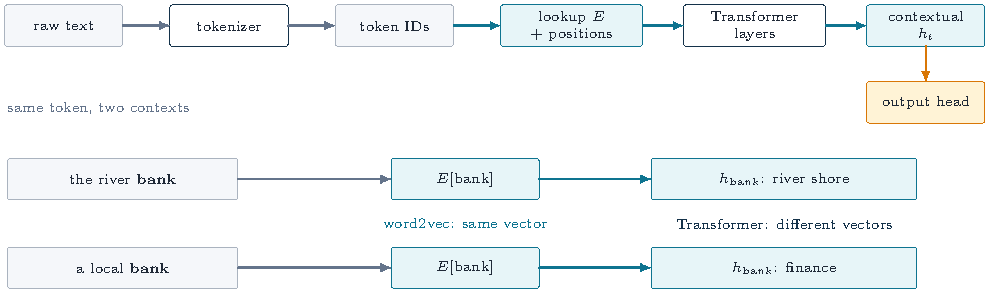
\includegraphics[width=\textwidth]{token_to_context.pdf}
\caption{自然语言输入到 Transformer 表示的路径。分词器把文字映射到词表编号，嵌入矩阵为编号提供初始向量；示例假设 \texttt{bank} 是一个 token，两句话查到相同的初始向量，经过上下文信息交换后得到不同的表示。输出头再把表示用于词表预测或具体任务。}
\label{fig:token-to-context}
\end{figure}

最早的 Transformer 用于机器翻译，采用编码器与解码器（Encoder--Decoder）两部分：先把完整源句编码，再根据源句表示逐步生成译文~\cite{vaswani2017attention}。后来广泛使用的两条路线是 BERT 主要使用编码器学习文本表示~\cite{devlin2019bert}；以及 GPT，使用只有因果解码层的网络学习序列生成~\cite{radford2018gpt}。图 \ref{fig:transformer-overview} 展示三种结构的信息流。

三条路线共享上述输入路径和层内骨架。\textbf{自注意力}让一个位置从可见的其他位置读取信息；\textbf{前馈网络}（Feed-Forward Network，FFN）在每个位置内部变换通道；\textbf{残差连接}把子层输出加回输入，归一化控制数值尺度。多层堆叠后，每个位置得到包含内容与上下文的表示。网络最后可以把这些表示投影到词表并做 softmax，以预测 token，也可以接分类等任务输出头。

\begin{figure}[H]
\centering
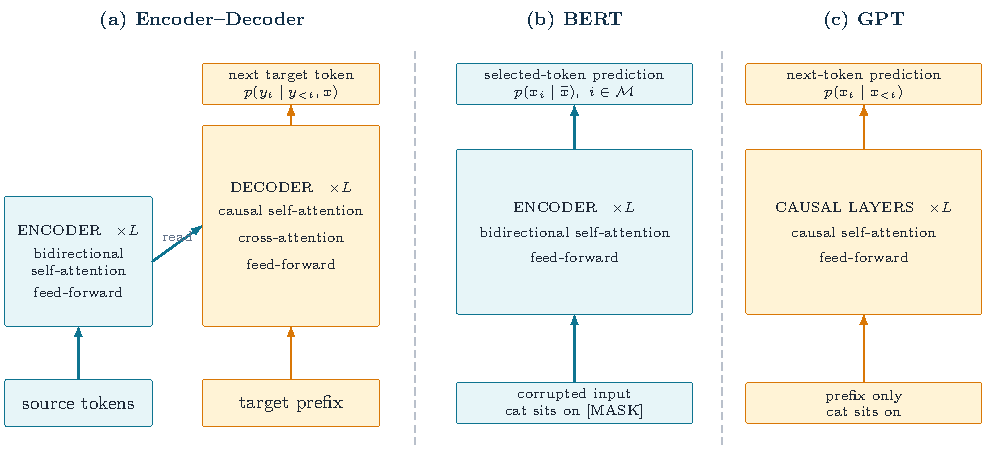
\includegraphics[width=\textwidth]{transformer_overview.pdf}
\caption{Transformer 的三种整体结构，箭头表示信息流。(a) 原始编码器读取完整源序列，解码器读取目标前缀，并通过交叉注意力访问源表示；(b) BERT 对经过遮盖或扰动的输入做双向编码，预测被选位置的原词；(c) GPT 只读取因果前缀，逐位置预测下一个 token。每个层框内部还包含残差连接与归一化。遮盖输入内容与限制注意力可见范围是两种不同操作。}
\label{fig:transformer-overview}
\end{figure}

\subsection{原始 Encoder--Decoder：先读源句，再写目标句}

设源句为 \(x_{1:S}\)，目标译文为 \(y_{1:T}\)。Encoder 的每一层包含双向自注意力和 FFN：源句已经完整给定，所以任意源位置都能读取其他源位置。堆叠后得到 \(H^{\mathrm{src}}=\operatorname{Encoder}(x_{1:S})\)，它是每个源位置的上下文表示。

Decoder 的每一层有三个子层：先用因果自注意力读取已经给定的目标前缀，再用\textbf{交叉注意力}读取 \(H^{\mathrm{src}}\)，最后经过 FFN。自注意力在“当前译文内部”交换信息，交叉注意力在“译文与源句之间”交换信息：当前译文表示决定要查找什么，编码器输出提供可查询的内容。因此解码器既知道自己写到哪里，也能随时回看源句。

词表投影与 softmax 把解码器输出变成条件概率，整台模型学习
\begin{equation}
 p_\theta(y_{1:T}\mid x_{1:S})
 =\prod_{t=1}^{T}p_\theta(y_t\mid y_{<t},x_{1:S}),\qquad
 \mathcal L_{\mathrm{translation}}
 =-\E_{(x,y)}\sum_{t=1}^{T}\log p_\theta(y_t\mid y_{<t},x_{1:S}).
 \label{eq:encoder-decoder-loss}
\end{equation}
训练时把真实目标序列右移一位送入 Decoder，使用 teacher forcing；因果遮罩使所有目标位置可以并行计算，却无法读取各自的正确答案。推理时先编码一次源句，再由解码器从 BOS 开始逐 token 生成，直到 EOS。这个结构适合“完整输入已经给定、输出需要依次产生”的条件生成任务。

\subsection{BERT：双向编码与遮盖词预测}
\label{sec:bert-mlm-link}

如果目标是分类、检索、句子匹配或抽取答案，通常希望一个词的表示同时利用左右两侧上下文。BERT 因此使用双向 Encoder。比如“他坐在河流的岸边”，后面的“河流”有助于确定前面相关词的含义；这种信息在整段文字已给定的任务中完全可用。

预训练又需要让这些表示从无标注文本中学到东西。若把原句完整输入，再要求每个位置输出它自己，模型很容易仅复制输入。遮盖语言建模（Masked Language Modeling，MLM）选择一部分位置集合 \(\mathcal M\)，将这些位置的输入遮盖或扰动，得到 \(\widetilde x\)，再让模型恢复原始 token：
\begin{equation}
 \mathcal L_{\mathrm{MLM}}
 =-\E_{x,\mathcal M,\widetilde x}\sum_{i\in\mathcal M}
 \log p_\theta(x_i\mid\widetilde x).
 \label{eq:bert-mlm}
\end{equation}
MLM 的损失只在被选中的位置计算。原始 BERT 的扰动机制除了替换为 \texttt{[MASK]}，也包括替换为随机 token 或保留原 token；因此“被选中预测的位置”与“实际显示 \texttt{[MASK]} 的位置”不必完全相同。例如输入“猫坐在 \texttt{[MASK]} 上”，目标是“垫子”，网络可以同时利用空缺两侧的信息；这就是完形填空目标与双向可见范围的配合。

原始 BERT 还加入下一句预测这一辅助任务：用分类汇总 token（Classification token，CLS）的表示判断两个句段是否在原文中相邻。若标签 \(b\in\{0,1\}\)，预测相邻的概率为 \(r_\theta\)，损失为
\begin{equation}
 \mathcal L_{\mathrm{sentence}}=-\E[b\log r_\theta+(1-b)\log(1-r_\theta)],\qquad
 \mathcal L_{\mathrm{BERT}}=\mathcal L_{\mathrm{MLM}}+\mathcal L_{\mathrm{sentence}}.
\end{equation}
这里的“下一句预测”是句段关系二分类；它不生成下一句。后续编码器模型可修改或去掉该辅助任务。预训练完成后，可以把 CLS 表示接分类头，或把各 token 表示接标注与答案位置预测头，再用具体任务的损失微调。

BERT 的填空条件分布利用了空缺左右的信息，MLM 因而没有直接给出从左到右的联合概率分解。若要生成一整段新文本，还需要另外设计填空顺序或迭代生成程序；第 \ref{sec:discrete-diffusion} 节的掩码扩散给出一种逐步恢复程序。下面 GPT 的目标则直接规定了从左到右的采样程序。

\subsection{GPT：因果解码与下一 token 预测}

GPT 采用 Decoder-only 结构。它保留因果自注意力、FFN、残差和归一化，并省去原始 Decoder 中读取独立 Encoder 输出的交叉注意力。提示词与生成结果放在同一条序列里，后面的位置只允许读取前面已经给出的内容。名称中的“Decoder”在这里描述这种因果序列结构，无需另配一个 Encoder。

考虑“猫、坐、在、垫子、上”这条序列。训练输入与标签错开一个位置：
\begin{equation}
 \begin{array}{c|cccccc}
 \text{输入}&\mathrm{BOS}&\text{猫}&\text{坐}&\text{在}&\text{垫子}&\text{上}\\
 \text{目标}&\text{猫}&\text{坐}&\text{在}&\text{垫子}&\text{上}&\mathrm{EOS}
 \end{array}.
\end{equation}
输入“在”的位置可以读取此前的“猫、坐”和当前“在”，预测下一个 token“垫子”。因果遮罩阻止它读取后面的“垫子”，所以标签不会通过注意力泄漏。所有位置都能同时产生这种预测，训练损失就是第 \ref{sec:autoregressive} 节的自回归 NLL：
\begin{equation}
 \mathcal L_{\mathrm{GPT}}=-\E_x\sum_{t=1}^{T}\log p_\theta(x_t\mid x_{<t}),\qquad
 p_\theta(x_{1:T})=\prod_{t=1}^{T}p_\theta(x_t\mid x_{<t}).
 \label{eq:gpt-next-token}
\end{equation}
预测“下一个词”更准确地说是预测下一个 token，它可能是完整词，也可能是子词或标点。这个目标直接来自联合概率的链式分解；生成时先采一个 token，再将其追加到前缀，重复使用同一个模型即可得到整段文本。GPT 系列的通用文本预训练沿用这一目标；指令微调通常只在回答部分计算相同的逐 token 损失，偏好优化与奖励训练则会增加或替换训练目标，第 \ref{chap:training-methods} 章再展开。

\subsection{结构、可见范围与训练损失的对应}

Encoder 和 Decoder 的层内骨架很相似，都使用自注意力、FFN、残差连接和归一化。就\textbf{自注意力的可见范围}而言，Encoder 中每个 token 可以读取所有输入 token；Decoder 的自注意力加上 causal mask（因果掩码），第 \(t\) 个位置只能读取自己和此前的 token。原始 Encoder--Decoder 架构中的 Decoder 还通过交叉注意力读取 Encoder 的输出。

BERT 做完形填空，是为了在双向上下文中学习恢复被扰动的内容；GPT 预测下一 token，是为了让训练时的条件与逐步生成时可得到的前缀一致。两者常用的逐位置损失都是词表上的交叉熵，区别主要在条件里能看到什么，以及在哪些位置计算损失。原始 Encoder--Decoder 也预测下一目标 token，但额外以完整源序列为条件（表 \ref{tab:transformer-objectives}）。

\begin{table}[ht]
\centering\small
\begin{tabularx}{\textwidth}{>{\bfseries}p{25mm} X X X}
\toprule
结构 & 当前预测可读取什么 & 典型预训练/训练目标 & 整台模型的用途\\
\midrule
Encoder--Decoder & 完整源序列与目标前缀 & 目标序列的条件 NLL & 翻译等序列到序列生成\\
BERT & 扰动后输入的左右上下文 & 被选位置的 MLM；原始版本另有句段关系损失 & 上下文表示与任务微调\\
GPT & 当前目标之前的 token & 各目标位置的下一 token NLL & 从前缀逐步生成新序列\\
\bottomrule
\end{tabularx}
\caption{三种结构的差别先体现在信息可见性与监督目标，内部都复用注意力和前馈网络。}
\label{tab:transformer-objectives}
\end{table}

接下来沿 GPT 使用的因果解码层展开内部组件。图 \ref{fig:transformer-overview} 中的一层由注意力、FFN、残差和归一化组成：注意力决定从哪些位置读取，位置编码补充顺序信息，FFN 组合通道特征，残差与归一化支持深层堆叠。

\section{查询、键、值与因果 mask}

给定序列表示矩阵 \(X\in\R^{T\times d}\)，其中 \(T\) 是本次送入模型的 token 数（序列长度），\(d\) 是每个 token 在残差流中的模型维度。单头投影通常把它映射到 \(Q,K\in\R^{T\times d_k}\) 和 \(V\in\R^{T\times d_v}\)；多头实现中常取 \(d_k=d_v=d/h\)，\(h\) 为 query head 数。这里的查询（Query，Q）、键（Key，K）和值（Value，V）分别表示“想找什么”“按什么匹配”和“读取什么”。于是
\begin{equation}
 Q=XW_Q,\quad K=XW_K,\quad V=XW_V,
\end{equation}
投影矩阵由训练学习。给定投影后的三个矩阵，单头注意力定义为
\begin{equation}
 \mathrm{Attn}(Q,K,V)=\softmax\left(\frac{QK^\top}{\sqrt{d_k}}+M\right)V,
\end{equation}
其中未来位置在 \(M\) 中设为 \(-\infty\)；以 \(X\) 为输入时，先用上式计算 \(Q,K,V\)，再代入 \(\mathrm{Attn}(Q,K,V)\)。

多头注意力（Multi-Head Attention，MHA）把上面这一步在各组投影上重复 \(h\) 次，再把结果拼回模型维度：
\begin{equation}
 \mathrm{head}_i=\mathrm{Attn}(XW_{Q,i},XW_{K,i},XW_{V,i}),\qquad
 \mathrm{MHA}(X)=\operatorname{Concat}(\mathrm{head}_1,\ldots,\mathrm{head}_h)W_O.
\end{equation}
这里 \(W_{Q,i},W_{K,i}\in\R^{d\times d_k}\)、\(W_{V,i}\in\R^{d\times d_v}\) 是第 \(i\) 个 head 自己的投影，因此每个 head 在自己的子空间里独立做一次内容寻址；\(W_O\in\R^{hd_v\times d}\) 是输出投影，把 \(h\) 个子空间的结果混合回 \(d\) 维残差流。单个 head 的表达能力有限，多头的作用是让模型同时维护多种不同的相似度度量。“拼接后投影”这一步不能省：没有 \(W_O\)，各 head 的输出只是并列拼在一起，无法互相组合。

这里每个符号都对应一个实际张量。\(X\) 的第 \(t\) 行是第 \(t\) 个 token 的隐藏向量；\(q_t\) 是“当前 token 想找什么”的 query，\(k_j\) 是“第 \(j\) 个 token 提供什么索引”的 key，\(v_j\) 是被读取的内容。矩阵 \(QK^\mathsf T\) 的第 \((t,j)\) 个元素是 query \(t\) 对 key \(j\) 的相似度，因果 mask 把 \(j>t\) 的位置变成 \(-\infty\)，softmax 后这些位置的权重为零；记权重矩阵为 \(A\)，则 \(AV\) 是对可见位置 value 的加权和，再经 \(W_O\) 回到残差流。训练时词表交叉熵的梯度沿 \(W_O\)、\(A\)、\(QK^\mathsf T\) 回传到 \(Q,K,V\) 及其投影权重。图 \ref{fig:causal-mask} 展示了哪些位置可见、哪些位置被遮盖。注意力权重反映这一层的读取模式，可以用来看模型在哪些位置交换信息。若关心某一层表示里是否包含某个物理量，可以在该层特征上训练一个线性探针，看它能否被线性读出。

\begin{figure}[ht]
\centering
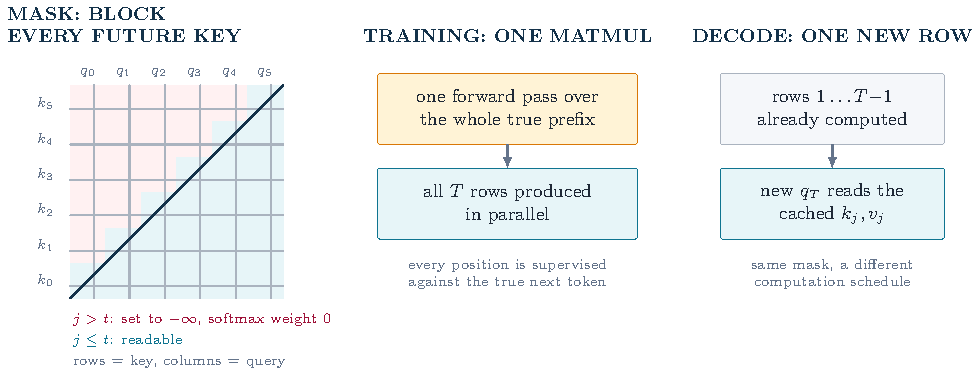
\includegraphics[width=\textwidth]{causal_mask.pdf}
\caption{因果自注意力的可见性与两种计算顺序。左：纵轴是 key 位置 \(k_j\)，横轴是 query 位置 \(q_t\)；对角线左上方 \(j>t\) 的格子设为 \(-\infty\)，softmax 权重为零。中：训练时一次前向并行算出注意力矩阵的全部 \(T\) 行（每个 query 一行）。右：解码时只有新的 \(q_T\) 读取缓存的 K/V；两者使用同一个 mask，只是计算顺序不同。}
\label{fig:causal-mask}
\end{figure}

\Needspace{10\baselineskip}
\section{注意力的几种变体：共享键值与汇总历史}

这里的“位置”是 token 在序列中的索引：\(t\) 表示当前要计算输出的 token，\(s\leq t\) 表示因果注意力可读取的第 \(s\) 个 token，其中 \(s<t\) 是先前 token，\(s=t\) 是当前 token。键 \(k_{s,i}\) 和值 \(v_{s,i}\) 由第 \(s\) 个 token 在本层的输入表示投影得到。前面的 MHA 有 \(h\) 个 query heads，每个 head 都用自己的 \(W_{Q,i},W_{K,i},W_{V,i}\) 投影，因此每个可见 token \(s\) 都为各 head 提供一组 \(k_{s,i},v_{s,i}\)。所谓\textbf{共享 K/V}，指多个 query heads 使用同一组 K/V 投影，读取同一个 token 时共用它的键和值；不同 token 的 K/V 仍然不同，query 投影也仍然按 head 区分。设第 \(i\) 个 query head 被分配到第 \(g(i)\) 组 K/V，其输出可以统一写成
\begin{equation}
 o_{t,i}=\sum_{s\le t}
 \frac{\exp\bigl(q_{t,i}^{\mathsf T}k_{s,g(i)}/\sqrt{d_k}\bigr)}
 {\sum_{r\le t}\exp\bigl(q_{t,i}^{\mathsf T}k_{r,g(i)}/\sqrt{d_k}\bigr)}
 v_{s,g(i)}.
\end{equation}
MHA 有 \(h\) 组 K/V，且 \(g(i)=i\)；多查询注意力（Multi-Query Attention，MQA）只有一组 K/V，所有 \(g(i)=1\)~\cite{shazeer2019mqa}；分组查询注意力（Grouped-Query Attention，GQA）保留介于两者之间的若干组，每组供多个 query heads 使用~\cite{ainslie2023gqa}。例如 8 个 query heads 配 2 组 K/V 时，每 4 个 query heads 共用一组 K/V 投影及其缓存。它们的 query 不同，所以即使读取同一组 K/V，softmax 权重和输出仍可不同。若有 \(n_{kv}\) 组 K/V，且各组维度相同，长度为 \(T\) 的已处理前缀需要保存约 \(Tn_{kv}(d_k+d_v)\) 个 K/V 数值；MQA 保存最少，GQA 居中，MHA 保留最多的 head 专属键值。共享减少了 K/V 缓存和生成时的读取量，也减少 K/V 投影参数，但 \(h\) 个 query heads 仍各自计算匹配权重，且共享越多，可供各 head 独立表达的前缀内容越少。

多头潜变量注意力（Multi-head Latent Attention，MLA）先把前缀中每个 token 的本层表示压成一个共享的低维向量，再由它生成各 head 所需的内容键和值，并另行处理位置相关信息~\cite{deepseekv2}。因此 MQA/GQA 是“多头共用几组键值”，MLA 是“每个 token 先存一份压缩表示，再供多头读取”；两者都保留按可见 token 做内容匹配和因果 mask。

\Needspace{7\baselineskip}
\textbf{局部窗口与少量全局 token。}另一种节省匹配次数的方式是稀疏注意力：普通 token 只读取邻近窗口及少量指定的全局 token，而全局 token 从较大范围读取并转递信息。Longformer 和 BigBird 用过这类结构处理长文档~\cite{beltagy2020longformer,zaheer2020bigbird}。其中“全局 token”是序列中的少数特殊 token；在自回归解码器中，它们的读写同样要遵守因果可见性，避免读到未来。另有局部层与全局层交替的做法：局部层只看滑动窗口，全局层让每个 token 查看完整可见前缀。这里的“全局”修饰整层的注意力范围，无需额外插入特殊 token。

\textbf{线性注意力：从 softmax 到递推状态。}先看一个注意力 head 在因果前缀上的输出。略去位置编码，普通 softmax 注意力可以写成
\begin{equation}
o_t^{\mathrm{softmax}}=
\frac{\sum_{s\le t}\exp\!\bigl(q_t^{\mathsf T}k_s/\sqrt{d_k}\bigr)v_s}
{\sum_{s\le t}\exp\!\bigl(q_t^{\mathsf T}k_s/\sqrt{d_k}\bigr)}.
\label{eq:softmax-causal-sum}
\end{equation}
每个历史位置的 value \(v_s\) 都按当前 query 与该位置 key 的匹配程度加权。新 query 到来时，分子和分母通常都要再次读取可见历史。

线性注意力保留“匹配后加权求和”这件事，但把指数匹配换成可拆开的非负内积~\cite{katharopoulos2020linear}。取固定维度 \(m\) 的特征映射 \(\phi:\R^{d_k}\to\R_{\geq0}^{m}\)，定义 \(a(q,k)=\phi(q)^{\mathsf T}\phi(k)\)。\(\phi\) 是对 query 和 key 的变换，例如逐元素使用指数线性单元（Exponential Linear Unit，ELU）构造 \(\operatorname{ELU}(x)+1\)；它不作用于 value。若 query 和 key 本来非负、\(\phi\) 取恒等映射，匹配权重就退化成 \(q^{\mathsf T}k\)。一般的 query 和 key 可以含负分量，直接去掉 softmax 而沿用原始点积会产生负权重或接近零的归一化分母；非负特征映射避免了这个问题，但新的权重通常不等于原来的 softmax 权重。

以这种基础形式为例，\(v_s\in\R^{d_v}\)。由于 \(\phi(q_t)\) 对求和中的每个历史位置都相同，可以把它移到求和外：
\begin{align}
o_t
&=\frac{\sum_{s\le t}\bigl[\phi(q_t)^{\mathsf T}\phi(k_s)\bigr]v_s}
{\sum_{s\le t}\phi(q_t)^{\mathsf T}\phi(k_s)+\varepsilon}
\label{eq:linear-attention-weighted}\\
&=\frac{\bigl(\sum_{s\le t}v_s\phi(k_s)^{\mathsf T}\bigr)\phi(q_t)}
{\bigl(\sum_{s\le t}\phi(k_s)\bigr)^{\mathsf T}\phi(q_t)+\varepsilon},
\qquad \varepsilon>0.
\label{eq:linear-attention-factored}
\end{align}
这里每个历史 token 对汇总状态贡献一项 \(v_s\phi(k_s)^{\mathsf T}\)：value 与变换后的 key 的外积。若 \(\phi\) 是恒等映射，它就是直观的 \(v_sk_s^{\mathsf T}\)；写出 \(\phi\) 是为了说明实际累加的是所选特征空间中的键值关联。

把上式两个与当前 query 无关的求和分别记为 \(S_t\) 和 \(z_t\)。新 token 到来时，只需在已有状态上增加它的一项，再用当前 query 读取：
\begin{align}
S_t&=S_{t-1}+v_t\phi(k_t)^{\mathsf T},\qquad S_0=0,\label{eq:linear-attention-state}\\
z_t&=z_{t-1}+\phi(k_t),\qquad z_0=0,\label{eq:linear-attention-normalizer}\\
o_t&=\frac{S_t\phi(q_t)}{z_t^{\mathsf T}\phi(q_t)+\varepsilon}.\label{eq:linear-attention-output}
\end{align}
\(S_t\in\R^{d_v\times m}\) 把 key 特征与 value 关联起来，\(z_t\in\R^m\) 保存归一化所需的特征总量。这里先把当前 \(k_t,v_t\) 写入状态，再用 \(q_t\) 读取，所以输出只依赖前 \(t\) 个 token（图 \ref{fig:linear-attention-state}）。

\begin{figure}[H]
\centering
\begin{tikzpicture}[node distance=12mm]
  \node[softblock,minimum width=27mm,minimum height=10mm] (past) {新 token\\\((k_t,v_t)\)};
  \node[tealblock,right=of past,minimum width=34mm,minimum height=10mm] (state) {固定大小的状态\\\(S_t,z_t\)};
  \node[softblock,right=of state,minimum width=23mm,minimum height=10mm] (read) {按查询读取};
  \node[softblock,right=of read,minimum width=17mm,minimum height=10mm] (out) {输出 \(o_t\)};
  \node[softblock,below=5mm of read,minimum width=23mm,minimum height=9mm] (query) {当前 \(\phi(q_t)\)};
  \draw[flow] (past) -- node[above,font=\scriptsize] {外积累加} (state);
  \draw[flow] (state) -- (read);
  \draw[flow] (query) -- (read);
  \draw[flow] (read) -- (out);
\end{tikzpicture}
\caption{每个新 token 把键值关联写入 \(S_t\)，当前 query 再从这份固定大小的状态读取。}
\label{fig:linear-attention-state}
\end{figure}

把 \(S_t\phi(q_t)\) 展开，就得到 \(\sum_{s\le t}v_s[\phi(k_s)^{\mathsf T}\phi(q_t)]\)。方括号中的内积衡量当前 query 与历史 key 在特征空间中的重合程度；重合越大，对应 value 在读出结果中的权重越大。\(z_t^{\mathsf T}\phi(q_t)\) 则汇总这些权重以完成归一化。因此 \(S_t\) 记住的是 key 与 value 的关联；多个 key 同时匹配时，读出的是相关 value 的加权混合。

当 \(m,d_v\) 固定时，更新和读取 \(S_t,z_t\) 的每步代价不随前缀长度增加，整段长度为 \(T\) 的序列所需的注意力计算随 \(T\) 线性增长。代价是多个 token 的键值关系合并在固定大小的状态中，不能像普通 softmax 注意力那样逐个寻址历史位置。

\Needspace{5\baselineskip}
从公开的自回归大模型看，保留可逐 token 寻址的 softmax 注意力及其窗口、GQA/MLA 或局部/全局层组合，仍比纯固定状态的线性注意力更常见：Mistral 7B 使用 GQA 与滑动窗口，Gemma 3 每五个局部注意力层配置一个全局注意力层~\cite{jiang2023mistral,gemmateam2025gemma3}。线性状态与可寻址注意力的混合也在发展，后文的 Kimi Linear 把 Kimi Delta Attention（KDA）层和 MLA 层交错使用~\cite{kimilinear}。

\begin{table}[H]
\centering\small
\begin{tabularx}{\textwidth}{>{\bfseries}p{28mm} X X}
\toprule
形式 & 历史信息怎样提供给 query & 主要取舍\\
\midrule
MHA & \(h\) 个 query heads 各有一组 K/V & 保留最多的 head 专属历史表示\\
MQA & \(h\) 个 query heads 共用一组 K/V & 历史存储最少，K/V 差异也最少\\
GQA & \(h\) 个 query heads 按组共用 K/V & 存储量与 K/V 多样性介于两者之间\\
MLA & 每个前缀 token 存低维向量，供各 head 生成 K/V & 压缩每个 token 的表示，增加投影步骤\\
局部窗口 + 全局 token & 普通 token 读窗口及少量全局 token & 保留稀疏的远程通道；因果生成需约束全局 token 的可见范围\\
局部层 + 全局层 & 局部层读窗口，全局层读完整可见前缀 & 保留按 token 寻址；全局层计算较重\\
线性注意力 & query 读取递推得到的 \(S_t,z_t\) & 状态大小固定，不能逐个寻址前缀 token\\
\bottomrule
\end{tabularx}
\caption{几种注意力形式的区别在于 query 能读取怎样的历史表示。}
\label{tab:attention-variants}
\end{table}

\section{Transformer 层的组件与词表输出}

\subsection{位置编码：绝对位置、RoPE 与 ALiBi}
\label{sec:rope}

位置编码解决的是自注意力本身对 token 排列置换不敏感的问题。绝对位置嵌入直接把一个可学习向量 \(p_t\) 加到 token 嵌入；它在训练长度内简单有效，但长度外推时没有未见过的位置向量。Rotary Position Embedding（RoPE）把每两维组成二维平面，在位置 \(m\) 施加旋转矩阵 \(R_{\theta,m}\)：
\begin{equation}
 q_m'=R_{\theta,m}q_m,\qquad k_n'=R_{\theta,n}k_n,\qquad
 (q_m')^\mathsf T k_n'
 =q_m^\mathsf T R_{\theta,n-m}k_n.
\end{equation}
最后一个等式说明内积依赖相对位置 \(n-m\)，这个依赖直接来自旋转角度的差。Attention with Linear Biases（ALiBi）保留 Q/K 原样，在 logit 中加入距离惩罚 \(b_h(m-n)\)~\cite{su2021rope,press2022alibi}。RoPE 的优势是保留多维相位关系，ALiBi 的优势是形式简单、距离偏置直接；两者都需要与训练长度、频率尺度和数值范围一起设计。

\subsection{归一化与残差连接}

层归一化（Layer Normalization，LayerNorm）对每个 token 的 \(d\) 维向量单独计算通道均值和方差，再把各通道的数值调整到稳定尺度，不在不同 token 之间求统计量。对 \(x\in\R^d\)，令 \(\mu(x)=d^{-1}\sum_jx_j\)、\(s^2(x)=d^{-1}\sum_j[x_j-\mu(x)]^2\)，则
\begin{equation}
 \operatorname{LayerNorm}(x)_j=\gamma_j\frac{x_j-\mu(x)}{\sqrt{s^2(x)+\varepsilon}}+\beta_j.
\end{equation}
其中 \(\varepsilon\) 是防止分母过小的固定常数；\(\gamma,\beta\in\R^d\) 分别是训练得到的逐通道缩放和偏移，每个 LayerNorm 层有 \(2d\) 个可训练参数。均值和方差由当前输入计算；同一层的 \(\gamma,\beta\) 在所有 token 位置共享。

对注意力或 FFN 子层 \(\mathcal F_l\)，Post-Norm 在残差相加后归一化，即 \(h_{l+1}=\operatorname{Norm}(h_l+\mathcal F_l(h_l))\)。Pre-Norm 先归一化子层输入，再把输出加回原始残差，即 \(h_{l+1}=h_l+\mathcal F_l(\operatorname{Norm}(h_l))\)。两者使用相同的归一化规则，差别在归一化的位置；图 \ref{fig:transformer-block} 左侧是一个 Pre-Norm block。Pre-Norm 给梯度提供更直接的残差路径，深层训练通常更稳定；均方根归一化（Root Mean Square Layer Normalization，RMSNorm）只用
\begin{equation}
\operatorname{RMSNorm}(x)_j=\gamma_j\frac{x_j}{\sqrt{d^{-1}\sum_kx_k^2+\varepsilon}},
\end{equation}
省去减去均值和可训练的偏移 \(\beta\)，每层仅保留 \(d\) 个缩放参数，相应减少计算和参数~\cite{zhang2019rmsnorm}。归一化在概率模型中承担的是尺度控制：让矩阵乘法、softmax 和残差叠加中的数值范围保持稳定。

\subsection{前馈网络：非线性与门控}

注意力负责位置之间的信息交换，FFN 负责把每个位置已收集的信息组合成新特征。若只堆叠线性映射，多层仍等价于一个线性映射；在升维与降维之间加入非线性，才能表达更复杂的特征组合。基本 FFN 为
\begin{equation}
 \operatorname{FFN}(h)=W_2\,\varphi(W_1h+b_1)+b_2,
\end{equation}
其中 \(d_{\mathrm{ff}}\) 是中间宽度，\(\varphi\) 是逐元素激活函数。高斯误差线性单元（Gaussian Error Linear Unit，GELU）的精确定义是 \(\varphi(x)=x\Phi(x)\)，其中 \(\Phi\) 是标准正态分布的累积分布函数；BERT 和视觉 Transformer 的前馈层都使用 GELU~\cite{devlin2019bert,dosovitskiy2021vit}。

现代模型中常用 sigmoid 线性单元（Sigmoid Linear Unit，SiLU）。它的具体函数是
\begin{equation}
 \sigma(x)=\frac{1}{1+e^{-x}},\qquad
 \operatorname{SiLU}(x)=x\sigma(x)=\frac{x}{1+e^{-x}}.
 \label{eq:silu}
\end{equation}
这里 \(\sigma\) 是 sigmoid 函数。SiLU 将输入乘以一个介于 0 和 1 之间的平滑系数：较大的正输入近似保留，较大的负输入趋于零，靠近零的负输入仍可通过。它在全域可微，且 \(\operatorname{SiLU}'(0)=1/2\)，所以零附近仍有梯度；通常所说的 Swish 在门控尺度取 1 时就是 SiLU。

单个激活函数只变换一个分支。门控线性单元（Gated Linear Unit，GLU）进一步使用两条投影：一条提供内容，另一条根据输入控制各通道的系数。SwiGLU（Swish Gated Linear Unit，Swish 门控线性单元）用 SiLU 处理门控分支~\cite{shazeer2020glu}：
\begin{equation}
 g=W_gh,\qquad u=W_uh,\qquad
 \operatorname{SwiGLU}(h)=W_d[\operatorname{SiLU}(g)\odot u].
 \label{eq:swiglu}
\end{equation}
\(W_g,W_u\) 将表示升到中间宽度，\(\odot\) 表示对应通道逐元素相乘，\(W_d\) 再投影回残差维度。门控让同一内容分支在不同输入下有不同的通道权重；门控分支的输出 \(\operatorname{SiLU}(g)\) 可以为负，也不限于 \([0,1]\)，因此它提供连续的可学习调制。训练梯度同时更新两个升维分支和降维矩阵。

\begin{figure}[ht]
\centering
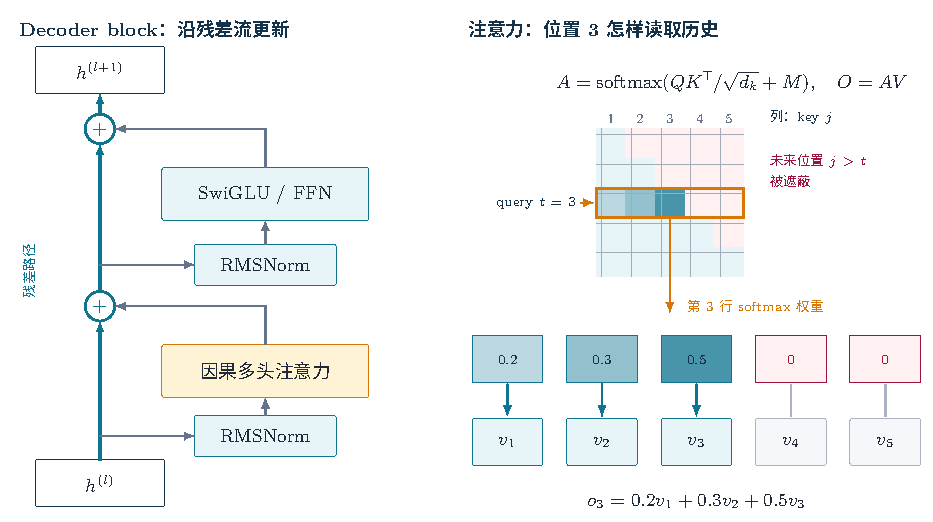
\includegraphics[width=\textwidth]{transformer_block_detailed.pdf}
\caption{一个 Pre-Norm decoder block 与一次因果注意力读取。左侧两条子层分支都从残差流取输入，计算后再加回；词表投影发生在堆叠的 block 之后。右侧以位置 3 为例：遮蔽未来位置，取注意力矩阵的第 3 行；等宽色块中的数字是示意权重，只有前三个 value 参与输出。}
\label{fig:transformer-block}
\end{figure}

\subsection{词表输出与训练、生成流程}

最后一个 block 的隐藏状态还不直接是概率。若位置 \(t\) 输入的是 \(x_t\)，那么 \(h_t^{(L)}\) 已经读取 \(x_{\le t}\)，用于预测 \(x_{t+1}\)；BOS 对应位置 \(t=0\)。模型先算出词表 logits
\begin{equation}
 l_t=W_{\mathrm{vocab}}h_t^{(L)}\in\R^{|\mathcal V|},
 \qquad
 p_\theta(x_{t+1}=v\mid x_{\le t})=\frac{\exp(l_{t,v}/\tau)}{\sum_{u\in\mathcal V}\exp(l_{t,u}/\tau)},
\end{equation}
其中 \(W_{\mathrm{vocab}}\in\R^{|\mathcal V|\times d}\) 是词表投影，往往与输入嵌入共享参数；\(\tau\) 在这里是采样温度，训练时取 \(\tau=1\)，此时这一行就是一个标准 softmax。所以“残差流中的向量”到“下一个 token 的概率”之间只有一次线性投影加一次 softmax，整个模型的输出维度就是词表大小 \(|\mathcal V|\)。

对一个长度为 \(T\) 的 batch，训练时把真实 token 序列一次送入网络；causal mask 使第 \(t\) 行只能使用 \(1,\ldots,t\) 的表示，各位置仍可并行计算。每个位置产生 logits \(l_t\)，softmax 给出词表分布，交叉熵取出真实下一个 token 的负对数概率，梯度再经过词表投影、FFN、注意力和输入嵌入传播。生成时把新 token 加入前缀，再计算下一个位置的条件分布；新的位置必须等待上一步的输出。

\section{解码：从 logits 到文本}
\label{sec:decoding}

模型给出的是每个位置上的条件分布 \(p_\theta(\cdot\mid x_{<t})\)；解码要做的是从中选一个 token，再把它接回前缀。选择方式会改变整条序列的分布，也会改变生成结果的多样性、重复程度和可复现性。下面按“是否保持模型分布”把常用做法分成几组。

\textbf{确定性与搜索。}贪心解码每一步取概率最大的 token。它可复现、延迟最低，代价是容易陷入重复循环，生成结果偏离 \(p_\theta\) 的联合分布。beam search 保留 \(B\) 条累计对数概率最高的部分序列，在每一步扩展后重新排序，最后取分数最高的一条。它近似寻找 \(p_\theta\) 下概率最高的序列，即分布的众数，结果是确定的，不对应 \(p_\theta\) 的随机样本；beam 越大，结果越保守，越容易偏向训练数据里常见的表达。对比解码（contrastive decoding）用一大一小两个模型的对数概率之差给 token 打分，压低小模型也会给高概率的通用、模板化 token~\cite{li2023contrastive}；DoLa（Decoding by Contrasting Layers）在同一模型内做类似比较，用深层与浅层输出的对数概率之差~\cite{chuang2023dola}。

\textbf{随机采样。}温度采样把 logit 除以 \(\tau\) 再做 softmax：\(\tau<1\) 使分布更尖，\(\tau>1\) 使分布更平。top-\(k\) 只保留概率最高的 \(k\) 个 token 后重新归一化；nucleus sampling（top-\(p\)）保留累计概率首次达到 \(p\) 的最小集合~\cite{holtzman2020curious}；min-\(p\) 保留概率不低于最大概率固定比例的 token；locally typical sampling 保留那些“信息量接近当前分布熵”的 token~\cite{meister2022typical}。这些操作都在改变分布：只有不截断且 \(\tau=1\) 时，逐步随机抽取才严格对应模型自身的 \(p_\theta(x)\)。

\textbf{惩罚项。}repetition penalty 对已经出现过的 token 降低 logit；frequency 和 presence penalty 按出现次数或是否出现来调整；no-repeat n-gram 直接禁止重复的 \(n\) 元组。它们都在 logits 上做加法或除法，因此同样改变分布。惩罚过强时，模型会回避必要的重复，例如化学式里的下标或代码里的括号，需要按任务调。

\textbf{约束解码。}如果输出必须符合某种结构，可以在每一步把不合法的 token 概率置零：正则表达式、JSON schema、语法都能编译成有限状态机，解码器只保留仍能走到合法终止状态的 token。这样得到的输出一定合法，但分布被限制在一个子集上，语言质量可能下降；约束越复杂，每步的掩码检查越贵。

\textbf{多采样与验证。}对同一问题独立生成多条回答，再用多数投票（self-consistency）或一个验证器挑选，属于推理时的额外计算~\cite{wang2023selfconsistency}。它改变的是最终交付的答案，模型分布保持不变；第 \ref{sec:test-time-scaling} 节的推理式扩展会回到这一点。

把上面几组放在一起，可以看出解码是“模型分布”与“任务约束”相遇的地方。表 \ref{tab:decoding-ops} 按“是否保持 \(p_\theta\)”归纳。

\begin{table}[H]
\centering\small
\begin{tabularx}{\textwidth}{>{\bfseries}p{40mm} p{30mm} X X}
\toprule
操作 & 改变发生在哪一步 & 作用 & 代价\\
\midrule
按模型分布采样（\(\tau=1\)、不截断） & 无，严格对应 \(p_\theta\) & 得到模型自身的样本 & 长尾与重复不受控\\
贪心 / beam search & 选择规则：退化为点估计或近似最大后验 & 稳定、可复现 & 容易重复、缺乏多样性；beam 计算量随宽度增加\\
温度、top-\(k\)、top-\(p\)、min-\(p\)、typical & 采样分布：平滑、截断或重归一化 & 控制多样性与生成长度 & 困惑度与校准不再对应 \(p_\theta\)\\
重复惩罚 & logit & 抑制循环 & 可能压掉必要的重复\\
约束解码 & 支撑集：限制在合法序列 & 保证输出符合语法或 schema & 质量可能下降\\
self-consistency / best-of-\(N\) & 最终答案的选择 & 提高最终答案的正确率 & 多次生成与评分\\
\bottomrule
\end{tabularx}
\caption{解码操作对分布的影响：只有不截断、\(\tau=1\) 的按分布采样保持 \(p_\theta\)；其余做法分别在选择规则、采样分布、logit、支撑集或最终答案上改变结果。}
\label{tab:decoding-ops}
\end{table}

\section{专家混合（Mixture of Experts，MoE）：把 FFN 换成稀疏路由}
\label{sec:moe}

普通 FFN 的所有参数都会对每个 token 执行计算。MoE 把这一子层换成多组独立的 FFN，称为专家，再让每个 token 只经过其中的 \(k\) 组~\cite{shazeer2017moe}。Switch Transformer 是每个 token 只选一个专家（\(k=1\)）的例子~\cite{fedus2022switch}。若有 \(N_{\mathrm{exp}}\) 个专家且 \(k\ll N_{\mathrm{exp}}\)，模型可以增加可选的参数总量，而单个 token 只执行选中专家的计算；注意力和残差路径仍按前面的方式工作。

\subsection{路由与容量}

路由器（router）读取当前位置表示 \(h_t\)，给每个专家一个分数并选出最高的 \(k\) 个：
\begin{equation}
 p_t=\operatorname{softmax}(W_rh_t),\qquad
 \mathcal S_t=\operatorname{TopK}(p_t,k),\qquad
 y_t=\sum_{e\in\mathcal S_t}\widetilde p_{t,e}\operatorname{FFN}_e(h_t).
\end{equation}
其中 \(W_r\in\R^{N_{\mathrm{exp}}\times d}\) 是可训练的路由矩阵，\(\widetilde p_{t,e}=p_{t,e}/\sum_{j\in\mathcal S_t}p_{t,j}\) 是选中专家之间的归一化权重。位置 \(t\) 的输出由这些专家的结果加权组合，再像普通 FFN 输出一样进入残差连接。

\(\operatorname{TopK}\) 决定“选谁”，这个离散选择本身不提供普通的连续梯度；在选中集合确定时，损失仍能通过 \(\widetilde p_{t,e}\) 更新路由器，并更新被选中专家的参数。未被选中的专家不会从该 token 得到主损失梯度。

实际执行还要给每个专家设一个容量上限。若一个 batch 有 \(B\) 个 token、\(N_{\mathrm{exp}}\) 个专家，容量常写成
\begin{equation}
 C=\text{capacity factor}\times\frac{B}{N_{\mathrm{exp}}},
\end{equation}
超出的 token 被丢弃，或者绕过专家直接沿残差路径通过。容量因子大于 1 留出余量，代价是显存和通信按容量预留；小于 1 则主动丢弃，吞吐稳定但质量下降。训练时可以用辅助损失让负载均匀，Switch Transformer 的形式是
\begin{equation}
 \mathcal L_{\mathrm{aux}}=N_{\mathrm{exp}}\sum_{e=1}^{N_{\mathrm{exp}}}f_eP_e,
 \label{eq:moe-aux}
\end{equation}
其中 \(f_e\) 是分给专家 \(e\) 的 token 比例，\(P_e\) 是该专家收到的平均路由概率~\cite{fedus2022switch}。它鼓励两者都接近 \(1/N_{\mathrm{exp}}\)。辅助损失与语言模型损失一起下降，系数太大会牺牲专家的专门化；DeepSeek-V3 改用一组按负载统计直接调整的选择偏置，不进入梯度，第 \ref{chap:modern-arch} 章会看到具体做法。

\subsection{共享专家与细粒度专家}

基础 MoE 让每个 token 在若干完整 FFN 之间选择。两种改动可以减少路由的浪费。一是把专家划得更细：用更多、更小的 FFN，每个 token 选更多个，组合数增加，而总计算量仍由 \(k\) 控制。二是保留一个所有 token 都经过的共享专家，让它承接各任务共有的变换，路由专家只负责差异部分~\cite{deepseekv2}。共享专家增加固定计算，但减少了路由专家需要重复学习的内容。

细粒度与共享专家一起用时，常见配置是“一个共享专家加多个细粒度路由专家”，每个 token 选其中少数几个。专家总数可以远大于单个 token 实际执行的专家数，参数量随之增加，但每 token 的浮点运算量仍接近一个稠密 FFN 的若干倍。

\subsection{专家并行与通信}

专家数量超过单卡容量后，不同专家被放到不同设备上，这就是专家并行（Expert Parallelism，EP）。路由器决定每个 token 去哪些设备，执行前把表示发送过去（dispatch），执行后把结果送回原位置（combine），两次都是 all-to-all 通信。若每个 token 选 \(k\) 个专家、表示宽度为 \(d\)、每个元素 \(b\) 字节，那么一个 token 往返的通信量约为 \(2kbd\) 字节；一个 batch 的总量再乘 token 数。

这条估算解释了后面几种设计。容量因子限制了单个设备一次要接收多少 token，负载不均会让某些设备成为等待的瓶颈；把路由分支压到低维潜空间（第 \ref{chap:modern-arch} 章的 Stable LatentMoE）相当于把上式中的 \(d\) 换成更小的 \(\ell\)；共享专家不经过路由，因此不产生跨设备流量。EP 通常与数据并行、张量并行和流水线并行组合使用，第 \ref{chap:training-stability} 章的多卡训练会把这些轴放在一起。

\chapter{多模态：理解与生成}
\label{chap:multimodal}

\begin{keybox}[两个方向，三个问题]
多模态模型有两个方向。理解方向把图像、视频或音频编码成表示，交给语言模型生成文字；生成方向以文字为条件，输出图像、视频或音频。两个方向都要回答三个问题：模态用什么 token 表示，条件从网络的哪个位置进入，用什么损失训练两者的对应关系。理解需要语义表示，生成需要能还原像素的表示，这一差别贯穿全章。
\end{keybox}

本章按信息流的顺序展开。第 \ref{sec:visual-tokens} 节把图像和视频变成 token 序列；第 \ref{sec:clip} 节用对比学习把图像与文本放进同一个表示空间，并从能量和互信息两个角度说明它优化的量；第 \ref{sec:vlm} 节把视觉 token 接进语言模型；第 \ref{sec:conditional-generation} 节反过来，以文本为条件生成图像和视频；第 \ref{sec:unified-multimodal} 节讨论把理解与生成放进同一个网络时遇到的矛盾。

\section{视觉 token 化：图像和视频怎样变成序列}
\label{sec:visual-tokens}

前面处理的是文字序列。要复用 Transformer 处理图像，需要先把二维像素变成一组向量，同时保留空间位置。视觉 Transformer（Vision Transformer，ViT）把图像切成固定大小的 patch，再把这些 patch 当作序列的 token。对大小为 \(H\times W\times 3\) 的图像，patch 边长为 \(P\) 时，patch 数为 \(N=(H/P)(W/P)\)；每个 \(P\times P\times3\) patch 展平成向量后，经线性投影变成 \(d_v\) 维 visual token~\cite{dosovitskiy2021vit}。另加入一个 CLS token，用于收集整幅图像的信息：
\begin{equation}
 u_i=W_{\mathrm{patch}}\operatorname{vec}(\operatorname{patch}_i)+b_{\mathrm{patch}},
 \qquad U_0=[u_{\mathrm{CLS}},u_1,\ldots,u_N]+P_{\mathrm{pos}}.
\end{equation}
其中 \(P_{\mathrm{pos}}\) 为位置向量。然后 \(U_0\) 进入普通 Transformer encoder。与语言 decoder 不同，ViT 使用双向自注意力：每个 patch 可以读取所有其他 patch；CLS token 的输出或所有 patch 的池化结果作为整幅图像的表示。训练目标可以是图像分类交叉熵，也可以是下一节的图文对比损失。

\textbf{分辨率与 token 数。}patch 数 \(N=HW/P^2\) 随分辨率平方增长，自注意力的计算和激活显存又随 \(N^2\) 增长。例如 \(P=14\) 时，\(336\times336\) 的图像给出 \(24\times24=576\) 个 patch，\(672\times672\) 的图像给出 2304 个。实际系统用两类办法控制 token 数。一是按图像的实际分辨率和长宽比决定 patch 网格，或把大图切成若干块分别编码，再附一张缩小的全图提供整体布局，避免统一缩放丢掉细节。二是在编码之后合并相邻 patch：把 \(2\times2\) 个相邻 patch 的特征拼成一个 \(4d_v\) 维向量，再用 MLP 投影回所需维度，token 数降为四分之一。合并保留了局部内容，只是每个 token 覆盖的面积变大；空间分辨率与 token 预算之间的取舍并没有消失。

\textbf{二维与时空位置。}语言序列只有一个位置下标，图像 patch 有行、列两个下标，视频 patch 还有帧号。第 \ref{sec:rope} 节的 RoPE 可以推广到多个下标。先把它的旋转矩阵写成分块形式：把每个 head 的 \(d\) 维 query 和 key 按相邻两维分成 \(d/2\) 个维度对，第 \(j\) 对记为 \(q^{(j)}=(q_{2j+1},q_{2j+2})\in\R^2\)（\(k^{(j)}\) 同理），配一个固定频率 \(\theta_j=b^{-2j/d}\)，常取 \(b=10^4\)。位置 \(m\) 处的旋转是块对角矩阵
\begin{equation}
 R_m=\diag\bigl(\rho(m\theta_0),\ldots,\rho(m\theta_{d/2-1})\bigr),
 \qquad
 \rho(\varphi)=\begin{pmatrix}\cos\varphi&-\sin\varphi\\ \sin\varphi&\cos\varphi\end{pmatrix}.
\end{equation}
二维旋转满足 \(\rho(\alpha)^\mathsf T\rho(\beta)=\rho(\beta-\alpha)\)，所以注意力 logit 按维度对拆成 \(d/2\) 项之和：
\begin{equation}
 (R_mq)^\mathsf T(R_nk)=\sum_{j=0}^{d/2-1}\bigl(q^{(j)}\bigr)^\mathsf T\rho\bigl((n-m)\theta_j\bigr)k^{(j)}.
 \label{eq:rope-pairs}
\end{equation}
每个维度对只感受到一个角度，即本对频率乘以位置差。

多模态旋转位置编码（Multimodal RoPE，M-RoPE）不改变维度对的划分，也不改变每一对的频率 \(\theta_j\)，只改变每一对旋转时乘的是哪个位置下标。位置换成三元组 \(p=(t,h,w)\)，分别是帧号、行号和列号；\(d/2\) 个维度对按编号分成连续的三组，第一组乘帧号 \(t\)，第二组乘行号 \(h\)，第三组乘列号 \(w\)。以 \(d=12\) 为例，6 个维度对的旋转角如下：
\begin{center}\small
\begin{tabular}{lcccccc}
\toprule
维度对 \(j\) & 0 & 1 & 2 & 3 & 4 & 5\\
对应的 query 分量 & \(q_1,q_2\) & \(q_3,q_4\) & \(q_5,q_6\) & \(q_7,q_8\) & \(q_9,q_{10}\) & \(q_{11},q_{12}\)\\
\midrule
一维 RoPE，位置 \(m\) & \(m\theta_0\) & \(m\theta_1\) & \(m\theta_2\) & \(m\theta_3\) & \(m\theta_4\) & \(m\theta_5\)\\
M-RoPE，图像 patch \((t,h,w)\) & \(t\theta_0\) & \(t\theta_1\) & \(h\theta_2\) & \(h\theta_3\) & \(w\theta_4\) & \(w\theta_5\)\\
M-RoPE，文本 token \((m,m,m)\) & \(m\theta_0\) & \(m\theta_1\) & \(m\theta_2\) & \(m\theta_3\) & \(m\theta_4\) & \(m\theta_5\)\\
\bottomrule
\end{tabular}
\end{center}
图像 patch 的前两对只随帧号转动，中间两对只随行号转动，最后两对只随列号转动。一般地，记三组的编号集合为 \(J_t,J_h,J_w\)，第 \(j\) 对的旋转角和整体旋转矩阵为
\begin{equation}
 \varphi_j(p)=
 \begin{cases}
 t\,\theta_j, & j\in J_t,\\
 h\,\theta_j, & j\in J_h,\\
 w\,\theta_j, & j\in J_w,
 \end{cases}
 \qquad
 R_p=\diag\bigl(\rho(\varphi_0(p)),\ldots,\rho(\varphi_{d/2-1}(p))\bigr).
 \label{eq:mrope}
\end{equation}
Qwen2-VL 中 \(d=128\)，64 个维度对按 16、24、24 分给 \(t,h,w\)~\cite{wang2024qwen2vl}。

logit 的“三段”来自式 \eqref{eq:rope-pairs} 的求和。那里的 \(d/2\) 项各对应一个维度对；把同一组的项归在一起，位置 \(p\) 的 query 与位置 \(p'\) 的 key 之间的 logit 就是
\begin{equation}
 (R_pq)^\mathsf T(R_{p'}k)
 =\sum_{j\in J_t}\bigl(q^{(j)}\bigr)^\mathsf T\rho(\Delta t\,\theta_j)k^{(j)}
 +\sum_{j\in J_h}\bigl(q^{(j)}\bigr)^\mathsf T\rho(\Delta h\,\theta_j)k^{(j)}
 +\sum_{j\in J_w}\bigl(q^{(j)}\bigr)^\mathsf T\rho(\Delta w\,\theta_j)k^{(j)},
\end{equation}
其中 \((\Delta t,\Delta h,\Delta w)=p'-p\)。在 \(d=12\) 的例子中，第一段是维度对 0、1 的两项，只含 \(\Delta t\)；第二段是维度对 2、3，只含 \(\Delta h\)；第三段是维度对 4、5，只含 \(\Delta w\)。所以 logit 只依赖两个 patch 在帧、行、列方向上的相对偏移。

文本 token 在第 \(m\) 个位置时取 \(p=(m,m,m)\)，表中最后一行与一维 RoPE 那一行完全相同：每一对都按 \(m\theta_j\) 旋转。三组用的仍是原来的全部频率 \(\theta_0,\ldots,\theta_{d/2-1}\)，三个下标又相等，所以分组不起作用，M-RoPE 在纯文本上退化为一维 RoPE。图文混排时，下标依次分配：例如前 5 个文本 token 占 \((0,0,0)\) 到 \((4,4,4)\)，随后一幅 \(2\times3\) patch 网格的图像，第 \(r\) 行第 \(c\) 列的 patch 取 \((5,\,5+r,\,5+c)\)；图像之后的文本从已用的最大下标加一，即 \((8,8,8)\) 开始。视频的不同帧依次增大 \(t\)。

\textbf{视频。}视频多了时间轴。把相邻 \(P_t\) 帧中同一位置的 \(P\times P\) 区域合成一个时空 patch，token 数为 \(N=(T/P_t)(H/P)(W/P)\)，\(P_t=1\) 时就是逐帧编码。帧数增加时 token 数线性增长，注意力代价按平方增长，因此视频理解通常先降低帧率或合并 token。

\textbf{音频。}音频的原始形式是一维波形 \(x[n]\)，采样率 24 kHz 时每秒有 24000 个采样值，直接当作 token 序列太长。常见的压缩表示有两种，见图 \ref{fig:audio-representations}：对数梅尔频谱是固定的信号变换，多用于语音识别等理解任务；神经音频编解码器是训练出来的表示，量化后成为离散 token，多用于生成。

\begin{figure}[t]
\centering
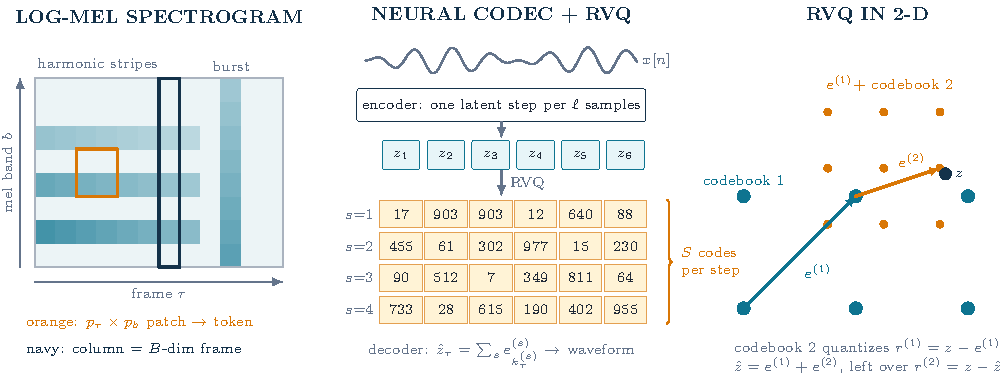
\includegraphics[width=\textwidth]{audio_representations.pdf}
\caption{音频的两种表示。左：对数梅尔频谱，横轴为帧，纵轴为梅尔频带；可以切二维 patch（橙框），也可以逐帧读出 \(B\) 维列向量（深蓝框）。中：编解码器每 \(\ell\) 个采样点输出一个潜在向量 \(z_\tau\)，残差向量量化把它变成 \(S\) 个编号，整段音频成为 \(S\times T\) 的整数网格。右：第一级选出离 \(z\) 最近的 \(e^{(1)}\)，第二级选出离残差 \(r^{(1)}=z-e^{(1)}\) 最近的 \(e^{(2)}\)，两者之和 \(\hat z\) 已接近 \(z\)。}
\label{fig:audio-representations}
\end{figure}

\textbf{对数梅尔频谱。}每隔 \(\ell\) 个采样点取一段长为 \(L\) 的加窗信号做傅里叶变换，把功率谱用 \(B\) 个梅尔滤波器 \(\Phi_{b,\kappa}\) 合并成频带，再取对数：
\begin{equation}
 Y_{\tau,b}=\log\Bigl(\sum_{\kappa}\Phi_{b,\kappa}\,|X_{\tau,\kappa}|^2+\varepsilon\Bigr),
 \qquad
 X_{\tau,\kappa}=\sum_{n=0}^{L-1}x[\tau\ell+n]\,w[n]\,e^{-2\pi\mathrm i\kappa n/L}.
\end{equation}
梅尔频带在低频窄、在高频宽，接近人耳的分辨率。\(Y\) 可以看成一幅图：横轴是帧 \(\tau\)，纵轴是频带 \(b\)，像素值是对数能量。它可以像 ViT 一样切成二维 patch，也可以把每一帧的 \(B\) 维列向量当作一个输入；Whisper 用后一种，每秒 100 帧，经卷积降采样后 30 秒音频成为 1500 个 token~\cite{radford2023whisper}。梅尔频谱丢掉了相位，用于生成时还需要声码器还原波形。

\textbf{神经音频编解码器与残差向量量化。}编解码器的卷积编码器每 \(\ell\) 个采样点输出一个潜在向量 \(z_\tau\)，解码器再把它们还原成波形，两者以重建损失和对抗损失联合训练~\cite{zeghidour2021soundstream,defossez2022encodec}。量化若只用一个含 \(M=1024\) 个码字的码本，每帧只有 10 比特，不足以高保真地重建声音。残差向量量化（Residual Vector Quantization，RVQ）用 \(S\) 个码本逐级量化，每一级量化前面各级留下的残差：
\begin{equation}
 r^{(0)}_\tau=z_\tau,\qquad
 k^{(s)}_\tau=\argmin_{j}\bigl\|r^{(s-1)}_\tau-e^{(s)}_j\bigr\|_2^2,\qquad
 r^{(s)}_\tau=r^{(s-1)}_\tau-e^{(s)}_{k^{(s)}_\tau},
 \qquad
 \hat z_\tau=\sum_{s=1}^{S}e^{(s)}_{k^{(s)}_\tau}.
 \label{eq:rvq}
\end{equation}
图 \ref{fig:audio-representations} 右侧是二维示意：\(z=(1.8,1.2)\)，第一级选中 \((1,1)\)，残差 \((0.8,0.2)\)；第二级选中 \((0.75,0.25)\)，残差缩小为 \((0.05,-0.05)\)。每一级本身就是第 \ref{sec:vector-quantized-latents} 节的向量量化（Vector Quantization，VQ）。每帧由 \(S\) 个编号表示，共 \(S\log_2M\) 比特；EnCodec 每秒 75 帧，取 \(S=8\) 时码率为 6 kbps。整段音频因此是 \(S\times T\) 的编号网格，按帧展开成序列时长度为 \(ST\)。

\textbf{理解用的表示与生成用的表示。}按训练目标，视觉 token 化可以分成两类，见表 \ref{tab:visual-tokenizers}。ViT 或图文对比预训练（Contrastive Language--Image Pre-training，CLIP）的图像编码器用分类或图文对比损失训练，只需保留区分语义所需的信息，没有解码器，输出不能还原成像素；它们是语言模型读取图像的入口。自编码器类 tokenizer，即第 \ref{sec:vector-quantized-latents} 节的 VQ-VAE 和潜空间扩散使用的自编码器，用重建损失训练，必须保留纹理和细节，并配有解码器；它们是生成模型工作的空间。前者擅长回答“图中是什么”，后者能把图画出来。同一套表示很难同时做好这两件事，这是第 \ref{sec:unified-multimodal} 节统一模型的核心难点。重建型 tokenizer 按输出形式又分两种。潜空间扩散的自编码器沿用第 \ref{chap:model-families} 章 VAE 的编码器—解码器结构，文献中通常直接称为 VAE；它输出连续向量网格，扩散直接在这些向量上进行。VQ-VAE 一类在同样的编码器之后再多一步量化，下文简称 VQ tokenizer：编码器把图像压成一个较小的向量网格，每个向量替换成码本中最近的码字，图像就变成一个整数编号网格，例如 \(512\times512\) 的图像变成 \(32\times32\) 个编号，可以像文本 token 一样排成序列做下一 token 预测；配套的解码器把编号网格还原成图像。

\begin{table}[ht]
\centering\small
\begin{tabularx}{\textwidth}{>{\bfseries}p{24mm} X X}
\toprule
 & 语义编码器 & 重建型 tokenizer\\
\midrule
训练目标 & 分类交叉熵或图文对比损失 & 像素重建，常加感知损失与对抗损失\\
输出 & 连续的 patch 向量 & 连续潜变量网格或离散码字网格\\
能否还原像素 & 不能，没有解码器 & 能，由解码器还原\\
保留的信息 & 与类别、文本描述相关的语义 & 纹理、边缘、颜色等局部细节\\
主要用途 & 视觉语言模型的视觉输入、检索、零样本分类 & 潜空间扩散、自回归图像生成\\
典型例子 & ViT、CLIP 图像编码器（第 \ref{sec:clip} 节） &潜空间扩散的自编码器、VQ-VAE\\
\bottomrule
\end{tabularx}
\caption{两类视觉表示。语义编码器服务于理解，重建型 tokenizer 服务于生成。}
\label{tab:visual-tokenizers}
\end{table}

\section{图文对比学习：对齐优化了什么}
\label{sec:clip}

图像向量和文本向量各自可用，但默认不在同一个语义空间。CLIP 通过让配对图文接近、非配对图文分开，建立可比较的表示；它使用一个 image encoder \(f_I\) 和一个 text encoder \(f_T\)，分别把图像 \(I_i\) 和配对文本 \(S_i\) 映射到同一个 \(d_c\) 维空间~\cite{radford2021clip}：
\begin{equation}
 u_i=\frac{f_I(I_i)}{\|f_I(I_i)\|_2},\qquad
 v_i=\frac{f_T(S_i)}{\|f_T(S_i)\|_2},\qquad
 \ell_{ij}=\frac{u_i^\mathsf T v_j}{\tau}.
\end{equation}
一个 batch 中其他图文对的文本就是负样本，\(B\) 个图像和 \(B\) 个文本构成一个 \(B\times B\) 的打分矩阵，对角线是真配对（图 \ref{fig:clip-example} 右）。图像到文本方向的交叉熵把 \(\ell_{ii}\) 推高、把 \(\ell_{ij}\)（\(j\neq i\)）压低；文本到图像方向再做一次对称的交叉熵：
\begin{equation}
 \mathcal L_{\mathrm{CLIP}}
 =\frac12\left[
 -\frac1B\sum_i\log\frac{\exp\ell_{ii}}{\sum_j\exp\ell_{ij}}
 -\frac1B\sum_i\log\frac{\exp\ell_{ii}}{\sum_j\exp\ell_{ji}}
 \right].
 \label{eq:clip-loss}
\end{equation}
归一化把训练重点放在向量间的角度，温度 \(\tau\) 控制相似度分布的尖锐程度。

\begin{figure}[t]
\centering
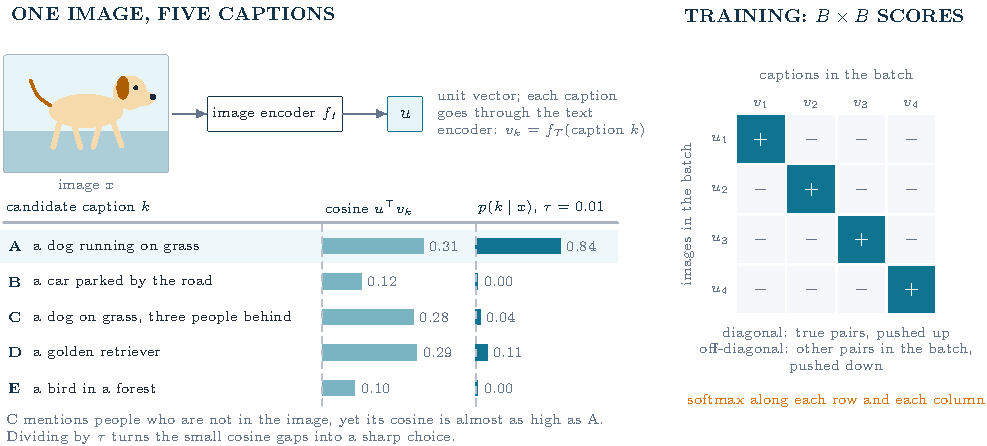
\includegraphics[width=\textwidth]{clip_example.pdf}
\caption{CLIP 在做什么。左：一张狗在草地上奔跑的图像经图像编码器得到 \(u\)，五条候选文本经文本编码器得到 \(v_k\)，逐一计算余弦相似度，再除以温度做 softmax。候选 C 提到了图中没有的三个人，余弦仍与 A 相差无几。右：训练时 batch 内的 \(B\) 张图像与 \(B\) 条文本两两打分，对角线上的真配对被推高，其余被压低。数值为示意。}
\label{fig:clip-example}
\end{figure}

训练完成后，图像与文本可以直接比较。图 \ref{fig:clip-example} 左侧是一个例子：同一张图像与五条候选文本分别计算余弦相似度，正确描述 A 得分最高。各候选的余弦只相差零点几，A 与 D 只差 0.02，但除以 \(\tau=0.01\) 后 logit 相差 2，概率相差约 \(e^2\approx7\) 倍。零样本分类就是这种比较：把每个类别名填进“一张\{类别\}的照片”这样的模板，经文本编码器得到 \(v_k\)，图像属于第 \(k\) 类的概率取为
\begin{equation}
 p(k\mid I)=\frac{\exp(u^\mathsf T v_k/\tau)}{\sum_{k'}\exp(u^\mathsf T v_{k'}/\tau)},
\end{equation}
不需要用这些类别的标注数据训练分类头。CLIP 学到的是整幅图像与整段文本之间的全局对应。它的局限也很明确：不擅长细粒度的空间关系、计数、图中文字和复杂的组合关系。图中候选 C 多出了图里没有的“三个人”，得分却几乎不降，就是这种局限的表现。

\textbf{能量与配分函数。}令 \(E_{ij}=-u_i^\mathsf T v_j\) 为图文对 \((i,j)\) 的能量。图像到文本方向第 \(i\) 行的损失可以写成
\begin{equation}
 \mathcal L_i=-\log\frac{e^{-E_{ii}/\tau}}{Z_i}=\frac{E_{ii}-F_i}{\tau},\qquad
 Z_i=\sum_{j=1}^{B}e^{-E_{ij}/\tau},\qquad
 F_i=-\tau\log Z_i .
\end{equation}
这是一个只有 \(B\) 个候选状态的正则系综：\(\tau\) 是温度，\(Z_i\) 是配分函数，\(F_i\) 是自由能。对参数求导得
\begin{equation}
 \nabla\mathcal L_i=\frac1\tau\Bigl[\nabla E_{ii}-\sum_j p_{ij}\nabla E_{ij}\Bigr],\qquad
 p_{ij}=\frac{e^{-E_{ij}/\tau}}{Z_i}.
\end{equation}
它与第 \ref{sec:ebm-mcmc} 节能量模型的梯度结构相同：第一项是正相位，降低真实配对的能量；第二项是负相位，按玻尔兹曼权重推高各候选配对的能量，与图像越相似的错误文本被推得越多。区别在负样本的来源：能量模型要用 MCMC 从模型分布中采样，CLIP 直接拿 batch 内的其他文本充当负样本，配分函数只在这 \(B\) 个候选上求和。温度越低，\(p_{ij}\) 越集中在最难区分的负样本上；CLIP 把 \(\tau\) 作为可学习参数。

\textbf{互信息下界。}式 \eqref{eq:clip-loss} 是两个方向的平均，这里只看图像到文本方向的那一半，另一方向同理。第 \(i\) 行对 \(B\) 条文本做 softmax，得到的 \(p_{ij}\) 与上一段相同：
\begin{equation}
 p_{ij}=\frac{\exp\ell_{ij}}{\sum_{k=1}^{B}\exp\ell_{ik}},\qquad
 \mathcal L_{\mathrm{InfoNCE}}=-\frac1B\sum_{i=1}^{B}\log p_{ii}.
 \label{eq:infonce}
\end{equation}
\(p_{ij}\) 可以读作模型认为“文本 \(j\) 是图像 \(i\) 的配对”的概率，损失就是真配对拿到的概率取负对数，再对 batch 平均。这种 batch 内 softmax 形式的对比损失称为 InfoNCE~\cite{vandenOord2018cpc}。

于是每一行都是一个猜谜游戏：给定一张图像，把概率分给 \(B\) 条候选文本，真配对分到的越多，损失越小。有两个参照点。全部押中真配对时 \(p_{ii}=1\)，损失为 0；编码器什么都没学到时，只能平均分配，\(p_{ii}=1/B\)，损失为 \(-\log(1/B)=\log B\)。实际损失介于两者之间，\(\log B-\mathcal L_{\mathrm{InfoNCE}}\) 衡量模型比随机猜好多少。例如 \(B=4\) 时（对数取自然对数，下同），随机猜的损失是 \(\log4\approx1.39\)；若模型对每张图像都给真配对 0.9 的概率，损失为 \(-\log0.9\approx0.11\)，比随机猜好 1.28。这个差值不会超过图像与文本之间的互信息：
\begin{equation}
 I(X;Y)\ge\log B-\mathcal L_{\mathrm{InfoNCE}}.
 \label{eq:infonce-bound}
\end{equation}
反过来读：训练把损失降到多少，就证明了图像与文本之间至少有多少互信息，上例中至少为 1.28。

对随机变量 \(Z_1\)，熵 \(H(Z_1)=\E[-\log P(Z_1)]\) 衡量对它的不确定度，在 \(B\) 个取值上均匀分布时为 \(\log B\)；条件熵 \(H(Z_1\mid Z_2)=\E[-\log P(Z_1\mid Z_2)]\) 是已知 \(Z_2\) 后剩下的不确定度。互信息是知道另一组变量后不确定度减少的量：
\begin{equation}
 I(Z_1;Z_2)=H(Z_1)-H(Z_1\mid Z_2),\qquad
 I(Z_1;Z_3\mid Z_2)=H(Z_1\mid Z_2)-H(Z_1\mid Z_2,Z_3).
\end{equation}
记号中分号隔开相比较的两边，逗号把几个变量合成一组，竖线后面是已知条件：\(I(Z_1;Z_2,Z_3)\) 是 \(Z_1\) 与 \((Z_2,Z_3)\) 这一组之间的互信息，条件互信息 \(I(Z_1;Z_3\mid Z_2)\) 是已知 \(Z_2\) 时 \(Z_3\) 还能提供的关于 \(Z_1\) 的信息。两种互信息都非负，且对分号两边对称。由定义直接得到链式法则 \(I(Z_1;Z_2,Z_3)=I(Z_1;Z_2)+I(Z_1;Z_3\mid Z_2)\)：一次看到 \((Z_2,Z_3)\) 得到的信息，等于先看 \(Z_2\) 得到的，加上已知 \(Z_2\) 后再看 \(Z_3\) 新增的。图像 \(X\) 与配对文本 \(Y\) 之间的互信息
\begin{equation}
 I(X;Y)=H(Y)-H(Y\mid X)=\E_{p(x,y)}\log\frac{p(y\mid x)}{p(y)}
\end{equation}
是看到图像后，对配对文本的不确定度平均减少了多少。

直观上，模型比随机猜好的部分只能来自线索，而线索只有一个来源：单看文本，\(B\) 条都像是从语料里随手抽出来的，分不出哪条特别；能把真配对挑出来的，只有它与图像之间的关联，其总量就是 \(I(X;Y)\)。严格地，只看第 \(i\) 行并打乱文本的顺序，softmax 不关心候选的排列，损失不变。于是真配对在一个均匀随机的位置 \(J\)：\((X,Y_J)\) 从 \(p(x,y)\) 中抽出，其余 \(B-1\) 条文本看作从 \(p(y)\) 中独立抽出，这里用大写字母表示随机变量。模型看到 \(D=(X,Y_{1:B})\)，给出猜测 \(q(J=j\mid D)=p_{ij}\)。

第一步，任何猜法都不比真实后验 \(P(J\mid D)\) 更好。交叉熵可以分解为熵加 KL 散度：
\begin{equation}
 \mathcal L_{\mathrm{InfoNCE}}=\E\bigl[-\log q(J\mid D)\bigr]
 =H(J\mid D)+\E_D\,\KL\bigl(P(\cdot\mid D)\Vert q(\cdot\mid D)\bigr)
 \ge H(J\mid D).
\end{equation}

第二步，比随机猜省下的不确定度就是互信息：\(\log B-H(J\mid D)=H(J)-H(J\mid D)=I(J;D)\)。与第一步合起来，\(\log B-\mathcal L_{\mathrm{InfoNCE}}\le I(J;D)\)。

第三步，线索不超过图像与文本共享的信息：
\begin{equation}
 I(J;D)=I(J;X\mid Y_{1:B})\le I(X;J,Y_{1:B})=I(X;Y).
\end{equation}
第一个等号用链式法则 \(I(J;D)=I(J;Y_{1:B})+I(J;X\mid Y_{1:B})\)，单看文本猜不出 \(J\)，\(I(J;Y_{1:B})=0\)。不等号再用一次链式法则，\(I(X;J,Y_{1:B})=I(X;Y_{1:B})+I(X;J\mid Y_{1:B})\)，多出的一项非负。最后一个等号换一种顺序展开，\(I(X;J,Y_{1:B})=I(X;J)+I(X;Y_{1:B}\mid J)\)：位置 \(J\) 与图像无关，第一项为 0；已知 \(J\) 时，与 \(X\) 相关的只有 \(Y_J\)，而 \((X,Y_J)\) 服从 \(p(x,y)\)，第二项等于 \(I(X;Y)\)。三步合起来就是式 \eqref{eq:infonce-bound}~\cite{poole2019variational}。证明没有用到编码器的任何性质；把图像和文本换成两个编码器的输出 \(u,v\)，同样的三步说明 \(\log B-\mathcal L_{\mathrm{InfoNCE}}\) 也是两个表示之间互信息的下界。

第一步的不等式在模型的猜测等于真实后验时取等号，由此可以求出打分 \(\ell_{ij}\) 在最优时学到的量。由贝叶斯公式，
\begin{equation}
 P(J=j\mid D)\propto p(y_j\mid x)\prod_{k\neq j}p(y_k)
 =\frac{p(y_j\mid x)}{p(y_j)}\prod_{k=1}^{B}p(y_k),
\end{equation}
连乘与 \(j\) 无关，所以真实后验正比于 \(p(y_j\mid x)/p(y_j)\)。softmax 的概率正比于 \(e^{\ell_{ij}}\)，两者一致要求打分为
\begin{equation}
 s^*(x,y)=\log\frac{p(y\mid x)}{p(y)}+c(x)=\log\frac{p(x,y)}{p(x)p(y)}+c(x),
\end{equation}
即逐点互信息，再加一个只依赖图像、在 softmax 中会约掉的常数。逐点互信息衡量看到图像后这条文本比平时可信了多少倍，而不是文本本身有多常见，所以“一张照片”这种对任何图像都适用的文本得分不会高。

这个下界给出两条结论。第一，损失非负，下界因而不超过 \(\log B\)：即使损失降到零，也只能证明 \(\log B\) 的互信息。CLIP 使用 32768 的 batch，\(\log B\approx10.4\)，大 batch 不只是加速手段，也决定了目标能分辨多少信息。第二，目标只奖励图像中与配对文本共享的信息。网络文本很少描述物体的精确个数、左右位置或图中小字，这些细节与文本的互信息很小，编码它们几乎不降低损失，全局对比学习也就没有动力保留它们。这正是上面所说的细粒度局限。

\textbf{sigmoid 版本。}语言图像预训练的 sigmoid 损失（Sigmoid Loss for Language Image Pre-training，SigLIP）把每个图文对看成独立的二分类~\cite{zhai2023siglip}：
\begin{equation}
 \mathcal L_{\mathrm{sig}}=-\frac1B\sum_{i,j}\log\sigma\bigl(z_{ij}(t\,u_i^\mathsf T v_j+b)\bigr),\qquad
 z_{ij}=\begin{cases}+1,&i=j,\\-1,&i\neq j,\end{cases}
\end{equation}
其中 \(t\) 是可学习的尺度，\(b\) 是可学习的偏置。它不对整行做 softmax，因而没有配分函数，相似度矩阵可以分块计算，对 batch 大小的依赖也比 softmax 版本小。逻辑回归的最优 logit 同样是逐点互信息，再加上正负样本先验比的对数；一个 batch 中正负样本之比约为 \(1:(B-1)\)，这部分由偏置 \(b\) 吸收，所以 \(b\) 通常初始化为较大的负值。两种损失学到的都是全局相似度接口，都不会自动得到 patch 与词语之间的精确对应。用这种损失训练出的图像编码器通常也直接叫 SigLIP 编码器；它和 CLIP 图像编码器一样是语义编码器，输出 patch 向量，是当前许多视觉语言模型的视觉部分。

\section{视觉语言模型：把视觉 token 接进语言模型}
\label{sec:vlm}

视觉语言模型（Vision--Language Model，VLM）读入一张图像和一段文字，输出文字，例如看图回答“左边是什么”。它的做法是把图像翻译成一串语言模型能读的向量，排在问题前面，让语言模型像读一段特殊的前缀那样读它。图 \ref{fig:vlm-architecture}(a) 画出了这个结构，它由三部分组成。视觉编码器通常就是上一节的 CLIP 或 SigLIP 图像编码器，它把图像切成 patch，为每个 patch 输出一个向量。这里保留全部 patch 向量，而不是只取一个全局向量，因为全局向量丢掉了物体在哪里，回答“左边是什么”恰恰需要空间信息。连接器（connector）通常只是一个小 MLP，把每个 patch 向量映射成语言模型输入空间中的 \(d\) 维向量，得到视觉 token \(v_{1:K}\)，token 数就是第 \ref{sec:visual-tokens} 节的 patch 数。连接器也可以把 token 数压到固定的 \(K\) 个：用 \(K\) 个可学习的 query 向量通过交叉注意力读取全部 patch 向量，每个 query 输出一个视觉 token，图像再大 \(K\) 也不变，BLIP-2 的 Q-Former 就是这样做的~\cite{li2023blip2}，代价是小字之类的细节可能在压缩中丢失。语言模型是一个普通的 decoder-only Transformer，它的输入是视觉 token 后面接文本 token，因果自注意力对两者一视同仁，回答逐 token 生成。

\begin{figure}[t]
\centering
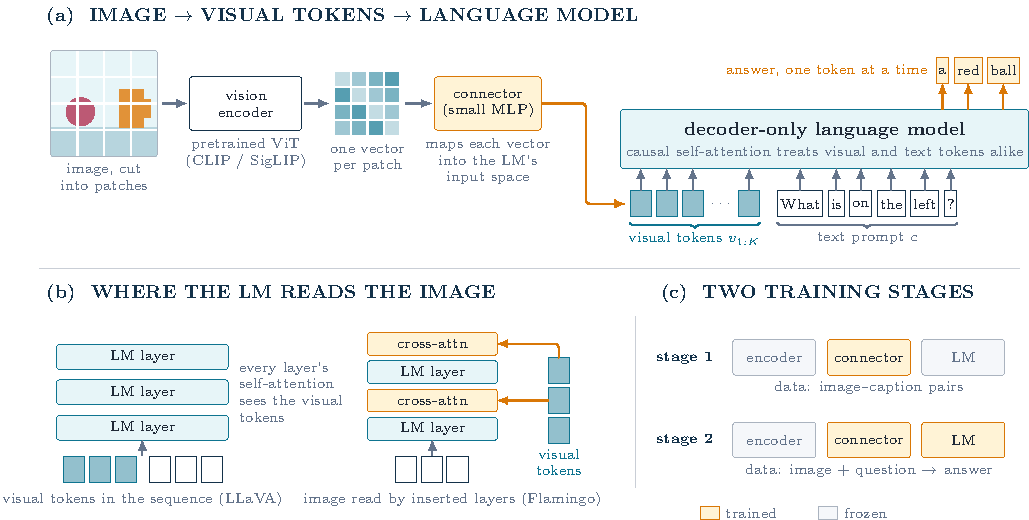
\includegraphics[width=\textwidth]{vlm_architecture.pdf}
\caption{视觉语言模型的结构。(a) 视觉编码器为每个 patch 输出一个向量，连接器把它们映射成视觉 token，排在文本提示前面送进语言模型，语言模型逐 token 生成回答。(b) 语言模型读取图像的两种方式：视觉 token 直接进入输入序列，或者留在序列之外，由插入的交叉注意力层读取。(c) 常见的两阶段训练：先只训练连接器，再连同语言模型一起微调。}
\label{fig:vlm-architecture}
\end{figure}

\textbf{语言模型在哪里读取图像。}图 \ref{fig:vlm-architecture}(b) 是两种方式。第一种是序列拼接：视觉 token 直接作为前缀放进输入序列，语言模型每一层的自注意力都能读到它们。LLaVA（Large Language and Vision Assistant）就是 CLIP 图像编码器加一个投影层，再接语言模型~\cite{liu2023llava}。语言模型的结构完全不变，这是它最大的优点，代价是视觉 token 占用序列长度，也一样写进 KV cache（第 \ref{sec:kv-budget} 节）。第二种是交叉注意力：图像不进入输入序列，而是在语言模型的层之间插入新的交叉注意力层，文字位置的隐状态作 query，视觉 token 作 key 和 value~\cite{alayrac2022flamingo}。它不占序列长度，但要新增层和参数。Flamingo 让每个新层的输出先乘一个初始为零的门控系数，训练开始时模型与原来的语言模型完全相同，之后再逐渐学会看图。

\textbf{训练。}VLM 的损失就是以图像为条件的下一 token 交叉熵：
\begin{equation}
\log p_\theta(y_{1:T}\mid v_{1:K},c)
=\sum_t\log p_\theta(y_t\mid y_{<t},v_{1:K},c),
\end{equation}
其中 \(c\) 是文本提示，\(y\) 是要生成的回答。损失的形式与语言模型相同，学到什么取决于数据，以及哪些部分参与更新。图 \ref{fig:vlm-architecture}(c) 是以 LLaVA 为代表的两阶段流程。第一阶段只训练连接器，视觉编码器和语言模型都冻结，数据是图像和它的描述。这一步相当于为连接器编一本词典，让映射后的视觉向量落在语言模型读得懂的位置。语言模型此时要冻结，因为刚初始化的连接器输出的是噪声，若语言模型跟着更新，已有的语言能力会受损。第二阶段做视觉指令微调，数据是“图像 + 问题 + 回答”，连接器和语言模型一起训练，损失只算在回答 token 上，与第 \ref{chap:training-methods} 章的监督微调（Supervised Fine-Tuning，SFT）相同。

\section{条件图像与视频生成}
\label{sec:conditional-generation}

生成方向把上一节的信息流倒过来：输入文字，输出像素。第 \ref{chap:model-families} 章已经给出了所需的生成算法：潜空间扩散和两种去噪网络（第 \ref{sec:diffusion-score} 节和图 \ref{fig:diffusion-denoiser}）、无分类器引导（式 \eqref{eq:cfg}），以及用 VQ-VAE 码字做自回归生成（第 \ref{sec:vector-quantized-latents} 节）。这一节不重复这些算法，只讨论多模态场景下新增的问题：在哪个表示空间生成，文本条件怎样编码，条件从哪里进入网络，以及视频带来的额外成本。

\textbf{在哪个空间生成。}在像素空间生成，每一步都要处理整幅图像。潜空间扩散先用表 \ref{tab:visual-tokenizers} 中的重建型自编码器把图像压成小得多的潜变量，例如 \(512\times512\times3\) 压成 \(64\times64\times4\)，去噪网络只在潜空间工作，细节由解码器补回~\cite{rombach2022ldm}。压缩率越高，生成越便宜，但解码器的重建质量成了整个系统的上限：自编码器还原不出的小字或细纹理，生成模型也画不出来。这也是这类自编码器要加感知损失和对抗损失的原因：只用像素均方误差训练时，解码器会对一组同样合理的细节取平均，重建就发糊~\cite{esser2021vqgan}。

\textbf{离散 token 的生成顺序。}若 tokenizer 输出离散码字，图像生成就成了序列生成。按光栅顺序逐个预测码字，可以直接复用语言模型，但一张 \(32\times32\) 的码字网格需要 1024 次串行调用，而且左上角生成时看不到右下角。MaskGIT 改为并行生成：从全部遮住开始，每一轮预测所有被遮住的位置，保留最有把握的一部分，其余重新遮住，约 8 轮即可完成~\cite{chang2022maskgit}。这就是第 \ref{sec:discrete-diffusion} 节的离散掩码扩散。

\textbf{文本条件怎样编码。}文本先经过一个通常冻结的文本编码器，得到一串 token 向量。早期的潜空间扩散使用 CLIP 文本编码器。Imagen 改用只在文本上预训练的 T5（Text-to-Text Transfer Transformer）编码器，发现增大文本编码器比增大扩散网络更能提高图文一致性~\cite{saharia2022imagen}。第 \ref{sec:clip} 节的互信息分析给出了解释：CLIP 文本编码器只被训练去保留有助于全局匹配的信息，对词序、数量和属性归属不敏感，比如分不清“红色的方块和蓝色的球”中哪个颜色属于哪个物体；在大量文本上训练的语言模型保留了更多句法结构。所以许多模型同时使用两类编码器~\cite{esser2024sd3}。

\textbf{条件从哪里进入网络。}文本 token 向量进入去噪网络有三种方式，前两种与上一节 VLM 的两种读取方式相同。交叉注意力让图像位置作 query、文本 token 作 key 和 value，U-Net 类去噪网络这样做（图 \ref{fig:diffusion-denoiser}）。序列拼接把文本 token 和图像 patch token 拼成一条序列做联合注意力，Stable Diffusion 3（SD3）这样做~\cite{esser2024sd3}。归一化调制把时间步、类别等条件压成一个向量，由它生成每层归一化的缩放和平移参数，DiT 用它注入时间步和类别标签~\cite{peebles2023dit}。前两种方式让每个图像位置都能读取每个文本 token，适合表达“左边红色、右边蓝色”这类逐位置的描述；调制对整幅图像施加同一组参数，只能表达全局属性，但最便宜。表 \ref{tab:condition-interfaces} 把理解与生成两个方向的注入方式放在一起比较。

\textbf{空间条件与编辑。}深度图、边缘图、人体姿态这类条件与图像处在同一空间网格上，可以逐位置对应，最简单的做法是把它们缩放到潜变量的分辨率，与带噪潜变量按通道拼接作为输入。修复就是这样做的：把掩码和保留区域拼进输入，模型只生成掩码内的内容。ControlNet 则不改动原网络：冻结预训练的去噪网络，复制一份可训练的分支读取条件图，分支的输出经初始化为零的卷积加回原网络~\cite{zhang2023controlnet}。训练开始时输出与原模型完全相同，这与 Flamingo 的零初始化门控是同一个思路：新加的条件通路从不起作用开始学，不破坏预训练得到的能力。

\textbf{视频。}视频生成在图像的基础上增加时间轴，成本主要来自 token 数。视频自编码器同时压缩空间和时间，但一段 4 秒的视频仍有同分辨率单张图像约 24 倍的 token。扩散的每一步都要对全部 token 做双向注意力，代价按 token 数的平方增长，24 倍的 token 意味着约 576 倍的注意力计算。常见的折中是分解注意力：一些层只在帧内做空间注意力，另一些层只在同一位置的不同帧之间做时间注意力，代价降为两部分之和，但跨帧、跨位置的交互要经过多层间接传递。让物体在运动中保持外观和形状一致，是视频生成相对图像生成新增的主要难点。

\begin{table}[ht]
\centering\small
\begin{tabularx}{\textwidth}{>{\bfseries\raggedright\arraybackslash}p{19mm} >{\raggedright\arraybackslash}X >{\raggedright\arraybackslash}p{22mm} >{\raggedright\arraybackslash}p{22mm} >{\raggedright\arraybackslash}X}
\toprule
接口 & 条件怎样进入 & 理解方向 & 生成方向 & 代价与表达能力\\
\midrule
序列拼接 & 条件 token 与主序列拼接，共用 self-attention & LLaVA、BLIP-2 的视觉前缀 & SD3 的文图联合注意力 & 序列变长，注意力按总长度平方增长；逐 token 双向交互\\
交叉注意力 & 主序列作 query，读取条件的 key 和 value & Flamingo & U-Net 读取文本 & 不占主序列长度，但增加层；条件表示不随主序列更新\\
归一化调制 & 条件压成一个向量，生成缩放、平移和门控参数 & 少用 & DiT 的时间步与类别 & 最便宜；只能表达全局属性\\
通道拼接 & 条件与输入逐位置对齐，按通道拼接 & 少用 & 修复掩码、深度图 & 要求同一空间网格；逐位置控制\\
全局相似度 & 两个编码器只在输出向量处比较 & CLIP 检索、零样本分类 & 不适用 & 最便宜；无细粒度交互，不能生成\\
\bottomrule
\end{tabularx}
\caption{条件注入接口。理解与生成两个方向共用前两种接口；它们的差别在于条件以多少个 token 出现，以及主网络在哪里读取它。}
\label{tab:condition-interfaces}
\end{table}

\section{统一多模态模型：理解与生成放进一个网络}
\label{sec:unified-multimodal}

前两节的理解模型和生成模型是分开的：VLM 读取语义编码器的输出，写出文字；图像生成模型在重建型潜空间中写出图像。统一模型想用一个 Transformer 在同一段上下文中既读又写，例如看图回答问题之后接着画一张修改后的图。设计时要回答两个问题。第一，读图和画图是否用同一种图像表示：语义编码器便于理解但不能还原像素，重建型 tokenizer 能画图但语义较弱（表 \ref{tab:visual-tokenizers}）。第二，图像以什么方式生成：VQ 码字可以像文字一样做下一 token 预测，连续的 VAE 潜变量则用扩散去噪。图 \ref{fig:unified-routes} 是三种有代表性的回答。

\begin{figure}[!tb]
\centering
\begin{tikzpicture}[x=1cm,y=1cm,font=\small,
  ttok/.style={draw=Teal,fill=Sky,minimum size=3.2mm,inner sep=0pt},
  dtok/.style={draw=Orange,fill=Amber,minimum size=3.2mm,inner sep=0pt},
  ctok/.style={circle,draw=Orange,fill=Amber,minimum size=3.2mm,inner sep=0pt},
  ubox/.style={draw=Navy,fill=white,rounded corners=2pt,minimum width=46mm,minimum height=9mm,align=center,font=\footnotesize},
  hbox/.style={ubox,minimum width=21mm},
  trunk/.style={ubox,fill=Mist},
  head/.style={font=\small\bfseries,color=Navy},
  cost/.style={font=\scriptsize,color=Slate,align=center}]
\begin{scope}
  \node[head] at (2.4,5.45) {(a) 全部离散化};
  \node[cost] at (2.4,5.05) {Chameleon};
  \node[ubox] (oa) at (2.4,4.25) {下一 token 预测\\图像码字 \(\to\) VQ 解码器};
  \node[trunk] (ta) at (2.4,2.95) {Transformer\\因果注意力};
  \foreach \i/\s in {0/ttok,1/ttok,2/ttok,3/dtok,4/dtok,5/dtok,6/dtok,7/ttok,8/ttok}
    \node[\s] at ({0.6+0.45*\i},1.75) {};
  \node[ubox] at (2.4,0.6) {VQ 编码器\\读图、画图共用};
  \draw[flow] (2.625,1.05)--(2.625,1.55);
  \draw[flow] (2.4,1.95)--(ta.south);
  \draw[flow] (ta.north)--(oa.south);
  \node[cost] at (2.4,-0.2) {理解只能依赖重建型码字};
\end{scope}
\begin{scope}[xshift=5.4cm]
  \node[head] at (2.4,5.45) {(b) 读写分用两种编码器};
  \node[cost] at (2.4,5.05) {Janus};
  \node[ubox] (ob) at (2.4,4.25) {下一 token 预测\\图像码字 \(\to\) VQ 解码器};
  \node[trunk] (tb) at (2.4,2.95) {Transformer\\因果注意力};
  \foreach \i/\s in {0/ttok,1/ctok,2/ctok,3/ctok,4/ttok,5/ttok,6/dtok,7/dtok,8/dtok,9/ttok}
    \node[\s] at ({0.51+0.42*\i},1.75) {};
  \node[hbox] at (1.2,0.6) {SigLIP 编码器\\用于读图};
  \node[hbox] at (3.6,0.6) {VQ 编码器\\用于画图};
  \draw[flow] (1.35,1.05)--(1.35,1.55);
  \draw[flow] (3.45,1.05)--(3.45,1.55);
  \draw[flow] (2.4,1.95)--(tb.south);
  \draw[flow] (tb.north)--(ob.south);
  \node[cost] at (2.4,-0.2) {同一张图有两种互不相同的表示};
\end{scope}
\begin{scope}[xshift=10.8cm]
  \node[head] at (2.4,5.45) {(c) 文字自回归，图像扩散};
  \node[cost] at (2.4,5.05) {Transfusion};
  \node[ubox] (oc) at (2.4,4.25) {文本：下一 token 预测\\图像：去噪 \(\to\) VAE 解码器};
  \node[trunk] (tc) at (2.4,2.95) {Transformer\\因果注意力，图内双向};
  \foreach \i/\s in {0/ttok,1/ttok,2/ttok,3/ctok,4/ctok,5/ctok,6/ctok,7/ttok,8/ttok}
    \node[\s] at ({0.6+0.45*\i},1.75) {};
  \node[ubox] at (2.4,0.6) {VAE 编码器，不量化\\读图、画图共用};
  \draw[flow] (2.625,1.05)--(2.625,1.55);
  \draw[flow] (2.4,1.95)--(tc.south);
  \draw[flow] (tc.north)--(oc.south);
  \node[cost] at (2.4,-0.2) {逐 token 解码与多步去噪交替进行};
\end{scope}
\node[ttok] at (3.2,-0.8) {};
\node[anchor=west,font=\footnotesize] at (3.4,-0.8) {文本 token};
\node[dtok] at (5.9,-0.8) {};
\node[anchor=west,font=\footnotesize] at (6.1,-0.8) {离散图像码字};
\node[ctok] at (8.9,-0.8) {};
\node[anchor=west,font=\footnotesize] at (9.1,-0.8) {连续图像向量};
\end{tikzpicture}
\caption{三种统一多模态模型。每栏自下而上：编码器把图像变成 token，与文本 token 拼成一条序列送入同一个 Transformer，顶部是训练目标和图像解码方式，最下方一行是主要代价。方块表示离散码字，圆点表示连续向量；VQ 编码器与 VAE 编码器的区别只在输出是否量化成码字（第 \ref{sec:visual-tokens} 节）。}
\label{fig:unified-routes}
\end{figure}

Chameleon 对两个问题都选统一：图像用 VQ 码字表示并入文本词表，读写都是下一 token 预测~\cite{chameleon2024}。图像从第一层起就与文字共享全部参数，没有独立的视觉编码器，这就是“早期融合”。代价是理解只能依赖语义较弱的重建型码字；图像 token 与文本 token 的统计性质差别也大，训练要靠查询与键归一化（Query--Key Normalization，QK-Norm；见第 \ref{sec:qk-norm} 节）等手段维持稳定。Janus 在第一个问题上分开：读图用 SigLIP 编码器（第 \ref{sec:clip} 节），画图仍预测 VQ 码字，代价是同一张图在模型中有两种表示~\cite{wu2024janus}。Transfusion 在第二个问题上改用扩散：图像以不量化的 VAE 潜变量进出网络，文本用下一 token 损失，图像用去噪损失；同一张图内部的 patch 互相可见，因为扩散一次去噪整幅图像~\cite{zhou2024transfusion}。它避开了量化损失，代价是推理时要在逐 token 解码与多步去噪之间切换。

原生多模态模型可以把同样的思路推广到语音：直接读写音频编解码器 token（第 \ref{sec:visual-tokens} 节），在文本、图像和音频上端到端训练。与“语音识别、语言模型、语音合成”三段级联的系统相比，语气、情绪和背景声不会在转写成文字时丢失，延迟也更低。

\chapter{训练方法：从预训练到可验证奖励}
\label{chap:training-methods}

\begin{keybox}[训练阶段改变的是同一个分布的哪一部分]
本章讨论的对象是自回归大语言模型，即前面推导过的 \(p_\theta(x_{1:T})=\prod_t p_\theta(x_t\mid x_{<t})\) 这一族模型。预训练用 MLE 在无标注语料上估计 \(p(x)\)；SFT（Supervised Fine-Tuning，监督微调）用成对的指令与答案把条件分布收缩到“回答问题”这一子集；人类反馈强化学习（Reinforcement Learning from Human Feedback，RLHF）和可验证奖励强化学习（Reinforcement Learning with Verifiable Rewards，RLVR）则改变输出的\textbf{相对权重}，让高奖励行为获得更多概率质量。推理训练进一步用解题轨迹或奖励强化生成中间步骤的行为。这些训练方式都沿用同一套自回归分解，差别在于经验分布 \(\hat\pi\) 由谁提供、以及目标里是否出现奖励项；蒸馏让另一个模型来提供这两者。
\end{keybox}

\begin{figure}[H]
\centering
\begin{tikzpicture}[node distance=7mm]
  \node[draw=Teal,fill=Sky,rounded corners=2mm,text width=41mm,minimum height=43mm,align=left,inner sep=3mm,font=\small] (base) {\textbf{1. 预训练：学会续写}\\[2mm]目标：预测下一个 token。\\[2mm]\texttt{Q: 1+1? A: 2}\\\texttt{Q: 2+2? A: 4}\\\texttt{Q: 3+3? A:}\\[1mm]{\scriptsize few-shot：示例写进提示。}};
  \node[draw=Navy,fill=Mist,rounded corners=2mm,text width=41mm,minimum height=43mm,align=left,inner sep=3mm,font=\small,right=7mm of base] (chat) {\textbf{2. 对话：SFT + RLHF}\\[2mm]用户：提出问题\\助手：给出回答\\[2mm]{\scriptsize SFT 学回答格式；RLHF 利用人类偏好改进回答。}};
  \node[draw=Orange,fill=Amber,rounded corners=2mm,text width=41mm,minimum height=43mm,align=left,inner sep=3mm,font=\small,right=7mm of chat] (reason) {\textbf{3. 推理：RLVR 等}\\[2mm]\texttt{<think>...}\\\texttt{</think>}\\最终答案：……\\[1mm]{\scriptsize RLVR 用程序可验证的正确性提供奖励。}};
  \draw[flow] (base.east)--(chat.west);
  \draw[flow] (chat.east)--(reason.west);
\end{tikzpicture}
\caption{自回归语言模型的交互形式路线图。SFT 建立对话格式，RLHF 使用人类偏好反馈，RLVR 使用可自动验证的奖励；各阶段都逐 token 生成。}
\label{fig:training-roadmap}
\end{figure}

图 \ref{fig:training-roadmap} 把两次\textbf{交互形式上的范式变化}连起来：从 Q/A 续写到用户/助手对话，再到在答案前生成 \texttt{<think>... </think>} 中间文本。预训练模型也可能在零样本提示下回答问题；few-shot 则把几组“Q: 问题，A: 答案”的示例放进前缀，利用续写完成新任务，本身不更新参数。SFT 用指令和合格回答训练稳定的问答行为，RLHF 等偏好优化再提高人们更认可的回答的概率。

RLHF 与 RLVR 的区别在反馈来源。RLHF 通常把人类对回答的比较训练成奖励模型，再用它优化对话策略；RLVR 用数学答案、代码测试等可自动判定的结果给奖励。二者都可调用后文的在线策略更新方法；推理训练还可以先用带中间步骤的 SFT 数据。

写出 \texttt{A:} 或 \texttt{<think>} 只是指定了输出格式，不会自动产生可靠的指令遵循或推理能力。相应能力仍要靠指令数据、偏好反馈、有效的推理轨迹或可验证奖励训练出来；显式写出的推理过程也需要独立检查，不能仅凭标签判断它是否正确。

\section{预训练：MLE 目标的实际形态}

预训练把大量无标注文本当作“给定前缀预测下一 token”的样本，用统计规律学习通用表示。其数学目标已在第 \ref{sec:autoregressive} 节给出：在语料经验分布 \(\hat\pi\) 上最小化负对数似然，等价于最小化 \(\KL(\hat\pi\Vert p_\theta)\)。实际系统中真正需要决定的是另外三件事，它们共同决定了模型最终能覆盖什么。

数据从哪来，决定了 \(\hat\pi\) 的形状。预训练语料通常由网页文本、代码、书籍、论文、百科和多语言内容混合而成。原始网页包含大量模板、广告、重复段落和机器生成文本，需要经过正文抽取、语言识别、长度与符号比例过滤、质量分类器打分和去重。去重分为完全重复和近似重复：前者用哈希，后者用 MinHash 或 n-gram 重叠；重复数据会让模型记住片段，也会让验证集与训练集重叠。代码和数学数据提供结构化推理的样本，比例过高会改变语言风格；合成数据可以补充稀缺格式，但需要保留真实数据作为锚点。第 \ref{chap:data-patterns} 章会把这些问题放在数据审计的框架里。

第一是\textbf{数据配比决定经验分布}。若语料由多个来源混合，\(\hat\pi=\sum_k\alpha_k\hat\pi_k\)，则改变权重 \(\alpha_k\) 就改变了被优化的目标，即使总 token 数不变。代码、数学、多语言和长文档的比例，本质上是在指定“哪些模式值得分配概率质量”。这与第 \ref{chap:data-patterns} 章的数据审计讨论的是同一件事，只是发生在训练之前。

第二是\textbf{规模配比}。参数量、训练 token 数和计算预算共同影响预训练效果；固定预算下，模型并非越大越好，还须给它足够的数据。第 \ref{sec:training-scaling} 节将用 scaling law 说明怎样配平这些规模，以及为什么实际部署有时选择另一种配比。

第三是\textbf{长程训练本身不稳定}。大规模预训练会出现 loss spike（损失突升）：某些 step 的梯度范数远超正常水平，若不加处理，可能让优化器状态被污染并使损失永久性变差。常见处理是回滚到 spike 之前的 checkpoint、跳过该 batch 的数据、临时降低学习率或收紧梯度裁剪阈值，同时用查询与键归一化（Query--Key Normalization，QK-Norm）、SwiGLU 输出限幅等结构约束（见后文表 \ref{tab:training-stability-mechanisms}）先把产生 spike 的路径收窄。

预训练给出的 \(p_0(x)\) 是一个通用文本分布的近似，它同时包含有帮助的续写、有害内容、错误陈述和格式混乱的输出，其中“回答问题”只是它覆盖的一小部分模式。把它转成能稳定遵循指令的模型，需要后面两个阶段。

\section{监督微调：数据、目标与参数适配}
\label{sec:sft}

\subsection{指令数据与回答损失}

SFT 的目标函数和预训练完全相同：
\begin{equation}
 \mathcal L_{\mathrm{SFT}}
 =-\E_{(c,y)\sim\mathcal D_{\mathrm{SFT}}}
 \sum_{t=1}^{T}\log p_\theta(y_t\mid y_{<t},c),
\end{equation}
其中 \(c\) 是指令或对话前缀，\(y\) 是期望的回答。变化的是数据集 \(\mathcal D_{\mathrm{SFT}}\)：它只包含“给定指令写出合格回答”的样本，而且损失通常只在回答 token 上计算，指令部分被 mask 掉。

因此 SFT 的机制是把条件分布 \(p_\theta(y\mid c)\) 的质量集中到人工认可的轨迹附近。它的局限也正来自这一点：训练数据里\textbf{只有正例，没有反例}。模型学到“这类回答是合理的”，但没有学到“另一类回答比它更差多少”。当同一个指令存在多个可接受答案、而它们的好坏有程度差别时，单纯的交叉熵无法表达这种比较关系。

SFT 还会继承 exposure bias：训练时前缀全部来自真实回答，部署时前缀来自模型自己。这也是为什么很多模型在短回答上表现良好，一旦自己写长了就开始偏离。

\subsection{参数适配：全参数微调与 LoRA}

SFT 规定了训练数据和损失，但还没有规定哪些参数随梯度更新。全参数微调从预训练权重 \(\theta_0\) 出发，更新注意力、FFN 等全部可训练参数；这样可调整的方向最多，却要为大量参数保存梯度和优化器状态，每个任务也可能需要一份完整的模型权重。参数高效微调的思路是冻结大部分预训练权重，只训练少量新增参数，让同一个基础模型适配不同任务。

低秩适配（Low-Rank Adaptation，LoRA）把一层原有矩阵 \(W_0\in\R^{d_{\mathrm{out}}\times d_{\mathrm{in}}}\) 冻结，在它旁边增加两个可训练的小矩阵~\cite{hu2022lora}：
\begin{equation}
 y=W_0x+\frac{\alpha}{r}BAx,\qquad
 A\in\R^{r\times d_{\mathrm{in}}},\quad
 B\in\R^{d_{\mathrm{out}}\times r},\quad
 r\ll\min(d_{\mathrm{in}},d_{\mathrm{out}}).
\end{equation}
这样待学习的权重变化是 \(\Delta W=(\alpha/r)BA\)，其秩至多为 \(r\)。直观上，这类似截断奇异值分解（Singular Value Decomposition，SVD）用较大奇异值对应的少数方向描述主要变化；LoRA 直接训练这两个低秩因子。原矩阵有 \(d_{\mathrm{out}}d_{\mathrm{in}}\) 个参数，这个 LoRA 分支只需训练 \(r(d_{\mathrm{in}}+d_{\mathrm{out}})\) 个；它可放在注意力投影或 FFN 矩阵上。训练时仍须让数据通过冻结的基础模型并反传到 LoRA 分支，主要节省的是可训练参数的梯度、优化器状态和任务专属权重的存储；推理时可把 \(\Delta W\) 并入 \(W_0\)。LoRA 沿用 SFT 的交叉熵目标；低秩约束限制了每层能做的改变，适合任务差异不大的适配。

\section{后训练：反馈来源与策略优化}
\label{sec:post-training}

\subsection{反馈来源与 KL 正则：后训练的共同目标}

SFT 只示范合格回答，后训练还需要判断哪个回答更好。这里先区分反馈来源：\textbf{RLHF} 从人类对回答的比较学习偏好，经典路线是用这些比较训练奖励模型，再用 PPO 在线更新语言模型；\textbf{RLVR} 用数学答案、代码测试等程序可验证的结果直接给奖励，常与 GRPO 等在线更新结合。PPO、GRPO 与留一法策略梯度（REINFORCE Leave-One-Out，RLOO）是怎样用奖励更新策略的方法；RLHF、RLVR 说明奖励从哪里来。直接偏好优化（Direct Preference Optimization，DPO）则直接学习固定的人类偏好对，属于离线偏好优化，不进行在线强化学习。

给定某种反馈得到的回答级奖励 \(r(x)\)，可以解一个带参考分布约束的优化问题：
\begin{equation}
 \max_q \; \E_{x\sim q}[r(x)]-\tau\,\KL(q\Vert p_0),
 \qquad\Longrightarrow\qquad
 q^*(x)\propto p_0(x)\exp\!\left(\frac{r(x)}{\tau}\right),\label{eq:kl-tilted-opt}
\end{equation}
式 \eqref{eq:kl-tilted-opt} 的最优解表明：奖励决定分布往哪个方向偏移，\(\tau\) 决定偏移多快，\(p_0\) 决定哪些区域本来就有概率质量——策略不可能凭空获得参考分布之外的行为。因此参考模型，也就是预训练模型，决定了后训练能到达的区域。

这个最优解可以直接验证。记 \(Z=\E_{p_0}[e^{r(x)/\tau}]\)，把右边的归一化分布记作 \(q^*=p_0e^{r/\tau}/Z\)，即 \(r=\tau\log(q^*/p_0)+\tau\log Z\)。代入目标，
\begin{equation}
 \E_q[r]-\tau\,\KL(q\Vert p_0)
 =-\tau\,\E_q\!\left[\log\frac{q}{p_0}-\frac{r}{\tau}\right]
 =-\tau\,\KL(q\Vert q^*)+\tau\log Z.
 \label{eq:kl-tilted-proof}
\end{equation}
\(\tau\log Z\) 与 \(q\) 无关，KL 非负且仅在 \(q=q^*\) 时为零，所以目标在 \(q^*\) 处取到最大值 \(\tau\log Z\)。统计学中把 \(p_0e^{r/\tau}/Z\) 称为 \(p_0\) 的指数倾斜（exponential tilting）：每个样本的权重乘以 \(e^{r/\tau}\) 再重新归一化。它也正是第 \ref{sec:free-energy} 节的变分自由能问题：令能量 \(E=-r\)、温度 \(T=\tau\)，并以 \(p_0\) 代替均匀测度，最大化上式就是最小化以 \(p_0\) 为参考的自由能，\(q^*\) 是对应的玻尔兹曼分布，\(-\tau\log Z\) 是自由能的最小值。两个极限也由此可读：\(\tau\to\infty\) 时 \(q^*\to p_0\)，奖励不起作用；\(\tau\to0\) 时 \(q^*\) 集中到 \(p_0\) 支撑内奖励最高的区域，按 \(p_0\) 的相对概率分配。

\begin{table}[H]
\centering\small
\begin{tabularx}{\textwidth}{>{\bfseries\raggedright\arraybackslash}p{30mm} >{\raggedright\arraybackslash}X >{\raggedright\arraybackslash}X}
\toprule
反馈路线 & 一批数据怎样得到分数 & 常见更新方法与适用任务\\
\midrule
RLHF：人类偏好 & 同一提示生成多个回答，由人比较优劣；可把偏好对训练成奖励模型，也可直接保存配对数据 & 经典在线路线是奖励模型 + PPO~\cite{ouyang2022instructgpt}；也可用 RLOO/GRPO 等无价值网络的在线更新。固定偏好对常用 DPO 做离线优化~\cite{rafailov2023dpo}。适合开放式对话、风格和安全偏好\\
RLVR：可验证奖励 & 同一题采样多个答案，由数值比对、单元测试或证明检查器给出正确性分数 & 常见在线路线是可验证奖励 + GRPO 等组相对更新~\cite{shao2024grpo,deepseekr1}；PPO 或 RLOO 也能接同样的奖励。适合数学、代码等可自动判题任务\\
AI 反馈：教师模型评判 & 同一提示生成多个回答，由更强的模型按评分细则打分或两两比较 & 分数接 GRPO、PPO 等在线更新，比较结果可接 DPO，见第 \ref{sec:distillation} 节。适合没有程序判题器、但有更强模型可用的开放任务\\
\bottomrule
\end{tabularx}
\caption{三类反馈来源和常见训练搭配。各路线不绑定某一种策略更新算法；DPO 使用固定的偏好对，不属于在线强化学习。}
\label{tab:posttraining-families}
\end{table}

\begin{keybox}[PPO 与 GRPO 的核心差别：逐位置优势还是整条轨迹优势]
本节讨论只有终局奖励的情况：两种方法都在完整回答结束后得到分数，但向生成 token 传递训练信号的粒度不同。\textbf{PPO} 额外训练一个 critic，让它对每个生成前缀预测未来回报；终局分数与各位置的预测相比较，形成随位置变化的优势，因此同一回答的不同 token 可以受到不同强度、甚至不同方向的鼓励或抑制。\textbf{GRPO} 不训练 critic，而以同一道题多条完整回答的平均得分作基线，给每条轨迹一个组相对优势，并把这个优势用于该轨迹的所有生成 token。选择的核心是是否学习\textbf{逐位置的优势信号}；GRPO 虽然共用轨迹优势，各 token 的概率比、裁剪和前缀仍会使最终梯度不同。
\end{keybox}

\subsection{PPO：逐位置优势与裁剪更新}

回答从当前策略 \(\pi_\theta\) 抽取，离散 token 的采样步骤不能沿可微生成路径回传；PPO 的策略更新因此使用第 \ref{sec:gradient-estimator-map} 节的 score-function 路径，以优势加权已选 token 的对数概率梯度。

强化学习（Reinforcement Learning，RL）把生成模型视为策略，把 token 视为动作，用回答获得的奖励调整动作概率。\textbf{奖励模型与 critic 各司其职：}经典 RLHF 先用人类偏好数据训练奖励模型 \(r_\psi(c,y)\)，让它对完整回答给一个分数；在随后的一轮 PPO 策略训练中，它通常冻结，只负责打分，不随策略梯度更新~\cite{stiennon2020learning,ouyang2022instructgpt}。它提供的是学习到的人类偏好近似；RLVR 则用同样固定的程序判题器代替奖励模型。

PPO 还要维护 critic \(V_\phi\)，它可以是独立网络，也可以是模型上的价值头。看一条实际训练样本：第 \(i\) 个提示是 \(c_i\)，策略模型生成回答 \(y_i=(y_{i,1},\ldots,y_{i,T_i})\)。准备写第 \(t\) 个 token 时，已有前缀 \(s_{i,t}=(c_i,y_{i,<t})\)；正在训练的 critic 输入这个前缀，输出一个标量 \(V_\phi(s_{i,t})\)，预测从这里继续生成的未来回报。完整回答写完后，冻结的奖励模型才输出终局分数 \(R_i=r_\psi(c_i,y_i)\)。忽略 KL 惩罚时，critic 要学的是从当前前缀续写到结束所得终局分数的条件期望，
\begin{equation}
 V_\phi(s_{i,t})\approx
 \E_{Y\sim\pi_\theta(\cdot\mid s_{i,t})}
 \bigl[r_\psi(c_i,y_{i,<t}Y)\bigr],
 \label{eq:ppo-critic-target}
\end{equation}
其中 \(Y\) 是续写部分；每批回答完成后，用观测到的终局分数回归这个预测。

先看本节只有终局奖励、且不折扣未来奖励的情况。回答 \(y_i\) 完成后，奖励模型给出的 \(R_i\) 用于该回答的每个生成位置；从它减去 critic 在写第 \(t\) 个 token 前输出的预测值，得到该 token 的采样优势估计 \(\widehat A_{i,t}\)：
\begin{equation}
 \widehat A_{i,t}:=R_i-V_\phi(s_{i,t}).
 \label{eq:ppo-terminal-advantage}
\end{equation}
\Needspace{4\baselineskip}
\(R_i\) 是完整回答的一次终局评分，对这条回答的所有位置相同；\(V_\phi(s_{i,t})\) 随生成前缀变化，因此各位置的 \(\widehat A_{i,t}\) 可以不同。策略损失用 \(\widehat A_{i,t}\) 加权第 \(t\) 个已选 token。若还要加入对参考模型的 KL 惩罚，各位置就不再只有末尾一个非零项；实际 PPO 常用广义优势估计（Generalized Advantage Estimation，GAE）把这些逐位置的数值和 critic 的预测结合起来计算 \(\widehat A_{i,t}\)，下文写出具体公式。

\Needspace{4\baselineskip}
有了优势，还要决定一批样本能被用几次。每轮先用当时的策略采样一批回答，并保存它在各个已选 token 上的概率，记为旧策略 \(\pi_{\mathrm{old}}\)；随后同一批回答用于多轮小批量更新，当前策略 \(\pi_\theta\) 逐渐偏离采样时的 \(\pi_{\mathrm{old}}\)。PPO 用概率比衡量这种偏离，并把它裁剪在 \([1-\varepsilon,1+\varepsilon]\) 内~\cite{schulman2017ppo}：
\begin{equation}
\begin{aligned}
 \rho_{i,t}(\theta)&=\frac{\pi_\theta(y_{i,t}\mid s_{i,t})}{\pi_{\mathrm{old}}(y_{i,t}\mid s_{i,t})},\\
 \mathcal L_{\mathrm{PPO}}(\theta)
 &=-\frac{1}{\sum_iT_i}\sum_{i}\sum_{t=1}^{T_i}
 \min\Bigl(\rho_{i,t}\widehat A_{i,t},\;
 \operatorname{clip}\bigl(\rho_{i,t},1-\varepsilon,1+\varepsilon\bigr)\widehat A_{i,t}\Bigr).
\end{aligned}
 \label{eq:ppo-clip}
\end{equation}
\(\varepsilon\) 常取 \(0.1\)--\(0.2\)。\(\widehat A_{i,t}>0\) 时，\(\rho_{i,t}\) 超过 \(1+\varepsilon\) 后目标不再增加，梯度为零；\(\widehat A_{i,t}<0\) 时，\(\rho_{i,t}\) 低于 \(1-\varepsilon\) 后同样停止。取 \(\min\) 使裁剪只截掉“朝有利方向走得过远”的那一侧，因此一批旧样本不能把策略推离 \(\pi_{\mathrm{old}}\) 太远。\(\rho_{i,t}\widehat A_{i,t}\) 看上去只是重加权，但它对 \(\theta\) 的梯度是 \(\widehat A_{i,t}\nabla_\theta\rho_{i,t}=\rho_{i,t}\widehat A_{i,t}\nabla_\theta\log\pi_\theta(y_{i,t}\mid s_{i,t})\)；在本轮开始的 \(\theta=\theta_{\mathrm{old}}\) 处 \(\rho=1\)，这正是第 \ref{sec:gradient-estimator-map} 节的 score-function 策略梯度。对数出现在求导之后；\(\rho\) 让同一批旧样本在后续小批量更新中继续近似这个梯度，裁剪限制这种近似的使用范围。与参考模型 \(\pi_{\mathrm{ref}}\) 的 KL 约束是另一层限制，下文写出 GAE 后再说明它加在哪里。critic 同时用均方误差更新参数 \(\phi\)：只有终局分数时，训练标签就是这条回答的 \(R_i\)，损失为 \((V_\phi(s_{i,t})-R_i)^2\)，对应式 \eqref{eq:ppo-critic-target}。奖励模型和 \(\pi_{\mathrm{ref}}\) 在这一阶段保持冻结。采集下一批回答时，才把更新后的策略保存为新的 \(\pi_{\mathrm{old}}\)。

前面提到的广义优势估计把各位置的时序差分向后累积。对第 \(i\) 条回答，
\begin{equation}
 \delta_{i,t}=r_{i,t}+\gamma V_\phi(s_{i,t+1})-V_\phi(s_{i,t}),\qquad
 \widehat A_{i,t}=\sum_{\ell=0}^{T_i-t}(\gamma\lambda)^\ell\delta_{i,t+\ell}.
 \label{eq:gae}
\end{equation}
这里 \(r_{i,t}\) 是 GAE 在第 \(t\) 个位置读入的逐位置信号，强化学习文献把它叫作即时奖励；本节称它为逐位置信号，以免与奖励模型的分数混淆。奖励模型只在回答写完后给一次分 \(R_i\)；\(r_{i,t}\) 不是奖励模型的输出，而是训练代码为 GAE 准备的一个长度为 \(T_i\) 的数组。只有终局分数时，这个数组前面全是零，只有最后一位 \(r_{i,T_i}=R_i\)。\(s_{i,T_i+1}\) 是写完的整条回答，之后不再有信号，其价值取零。\(\gamma\) 折扣较远的回报，\(\lambda\) 控制后续差分传回当前位置的程度：\(\lambda=0\) 只用当前一步，\(\lambda=1\) 传回整条轨迹。取 \(\gamma=\lambda=1\) 时，相邻两项的价值相互抵消：
\begin{equation}
 \widehat A_{i,t}
 =\sum_{t'=t}^{T_i}\bigl[r_{i,t'}+V_\phi(s_{i,t'+1})-V_\phi(s_{i,t'})\bigr]
 =\sum_{t'=t}^{T_i}r_{i,t'}-V_\phi(s_{i,t}),
 \label{eq:gae-lambda1}
\end{equation}
只剩从位置 \(t\) 到结尾的信号之和减去当前价值。只有终局分数时，信号之和就是 \(R_i\)，于是回到式 \eqref{eq:ppo-terminal-advantage} 的 \(\widehat A_{i,t}=R_i-V_\phi(s_{i,t})\)。

\textbf{KL 加在逐位置信号 \(r_{i,t}\) 上。}奖励模型本身不变，仍只给终局分数 \(R_i\)。经典 RLHF 实现改的是上面那个数组：原来为零的各位置填入一个 KL 惩罚，最后一位在 KL 惩罚之外再加上 \(R_i\)~\cite{ouyang2022instructgpt}，
\begin{equation}
 r_{i,t}=-\beta\log\frac{\pi_{\mathrm{old}}(y_{i,t}\mid s_{i,t})}{\pi_{\mathrm{ref}}(y_{i,t}\mid s_{i,t})}+\mathbf 1[t=T_i]\,R_i .
 \label{eq:ppo-kl-reward}
\end{equation}
其中 \(R_i=r_\psi(c_i,y_i)\) 仍是奖励模型给第 \(i\) 条完整回答的终局分数，指示函数 \(\mathbf 1[t=T_i]\) 只在最后一个位置取 \(1\)，所以 \(R_i\) 只加在末位。对数比由采样时保存的 \(\pi_{\mathrm{old}}\) 概率和冻结的 \(\pi_{\mathrm{ref}}\) 概率算出，在这一轮更新中是常数。优势和价值都不另加 KL 项，它们通过 \(r_{i,t}\) 间接带上 KL。把这个数组代入式 \eqref{eq:gae}，就得到含 KL 的优势；\(\gamma=\lambda=1\) 时直接用式 \eqref{eq:gae-lambda1}，
\begin{equation}
 \widehat A_{i,t}
 =R_i-\beta\sum_{t'=t}^{T_i}\log\frac{\pi_{\mathrm{old}}(y_{i,t'}\mid s_{i,t'})}{\pi_{\mathrm{ref}}(y_{i,t'}\mid s_{i,t'})}-V_\phi(s_{i,t}).
 \label{eq:ppo-kl-advantage}
\end{equation}
它比只有终局奖励时的 \(R_i-V_\phi(s_{i,t})\) 多出从位置 \(t\) 到结尾的 KL 累计；只累计 \(t\) 之后的项，是因为位置 \(t\) 的选择改变不了此前已写出的 token。critic 的训练标签相应改为从位置 \(t\) 到结尾的信号之和
\begin{equation}
 G_{i,t}=\sum_{t'=t}^{T_i}r_{i,t'}=R_i-\beta\sum_{t'=t}^{T_i}\log\frac{\pi_{\mathrm{old}}(y_{i,t'}\mid s_{i,t'})}{\pi_{\mathrm{ref}}(y_{i,t'}\mid s_{i,t'})},
 \qquad
 \mathcal L_V(\phi)=\bigl(V_\phi(s_{i,t})-G_{i,t}\bigr)^2 .
\end{equation}
\(G_{i,t}\) 由采样数据算出，是一个固定的数。一般的 \(\lambda<1\) 时，实现中常取 \(G_{i,t}=\widehat A_{i,t}+V_{\mathrm{old}}(s_{i,t})\)，其中 \(V_{\mathrm{old}}\) 是计算优势时 critic 的输出，同样作为常数，不随 \(\phi\) 变化；\(\lambda=1\) 时两种写法一致。标签里含 KL 项，所以 \(V_\phi\) 学到的是扣除 KL 后的期望回报，不再是式 \eqref{eq:ppo-critic-target} 中单纯的终局分数期望。归纳起来，KL 直接加在 \(r\) 上，经 GAE 进入 \(\widehat A\)，经训练标签 \(G\) 进入 \(V\)；式 \eqref{eq:ppo-clip} 用的 \(\widehat A_{i,t}\) 已经包含它，所以那里不必再写单独的 KL 项。KL 惩罚因此完全通过 \(\widehat A_{i,t}\) 的数值影响更新：一个 token 之后的续写偏离参考模型越多，它的优势越小，概率被抬高得越少，甚至被压低。第 \ref{sec:kl-placement} 节解释这样做为什么等价于 KL 正则目标，并与 GRPO 的放法比较。

PPO 需要额外训练 critic；若配合 RLHF 的奖励模型，还要承担奖励模型的误差。策略会主动搜索后者的高分区，可能从“回答更好”漂移到“更符合奖励模型的刻板特征”，形成 reward hacking。KL 项只能限制漂移幅度，不能修正奖励本身的偏差。

\subsection{GRPO/RLOO：组相对优势与留一基线}

GRPO/RLOO 同样沿第 \ref{sec:gradient-estimator-map} 节的 score-function 路径更新离散 token 的生成概率；它们改变的是用于加权对数概率梯度的优势。

当同一问题能采样多个答案时，可以用答案之间的分数差作基线，省去训练 critic 的成本。同一个问题上采样 \(G\) 个完整回答，同一个冻结的奖励模型或判题器先分别给它们打分 \(r_1,\ldots,r_G\)。GRPO 用组内均值作 baseline，并常按组内标准差归一化；RLOO 则对每条回答使用其余 \(G-1\) 条回答的平均奖励作 baseline~\cite{shao2024grpo,ahmadian2024rloo}：
\begin{equation}
 A_i^{\mathrm{GRPO}}=\frac{r_i-\operatorname{mean}(r_1,\ldots,r_G)}{\operatorname{std}(r_1,\ldots,r_G)+\delta},\qquad
 A_i^{\mathrm{RLOO}}=r_i-\frac{1}{G-1}\sum_{j\neq i}r_j,
 \label{eq:grpo-advantage}
\end{equation}
其中小常数 \(\delta\) 防止全组同分时除零。高于组内基线的轨迹优势为正，低于基线的为负。这个轨迹优势代替 PPO 的逐位置 \(\widehat A_{i,t}\)，放进同样的裁剪目标，并直接加上对参考模型的 KL 项：
\begin{equation}
 \mathcal L_{\mathrm{GRPO}}(\theta)
 =-\frac1G\sum_{i=1}^{G}\frac1{T_i}\sum_{t=1}^{T_i}
 \Bigl[\min\Bigl(\rho_{i,t}A_i,\;\operatorname{clip}(\rho_{i,t},1-\varepsilon,1+\varepsilon)A_i\Bigr)
 -\beta\,\widehat{\KL}_{i,t}\bigl(\pi_\theta\Vert\pi_{\mathrm{ref}}\bigr)\Bigr],
 \label{eq:grpo-loss}
\end{equation}
\(\rho_{i,t}\) 与式 \eqref{eq:ppo-clip} 相同，\(\widehat{\KL}_{i,t}\) 是在已采样 token 上估计的逐位置 KL，具体形式见下一小节。与 PPO 相比只改了两处：优势按轨迹而非按位置给出，KL 从奖励里移到了损失里。同一个 \(A_i\) 乘到这条轨迹所有生成 token 的对数概率项上，使整条高分轨迹更常出现、整条低分轨迹更少出现；各 token 的实际梯度仍因概率比、裁剪、KL 和所处前缀而不同。GRPO 省掉了 critic 的显存与学习误差；代价是终局分数无法指出轨迹内部哪一步真正起了作用，且每道题要采样多条回答。若把程序判分换成人类偏好奖励，它同样能用于在线 RLHF。

组相对仍然是在线方法：每步都要重新采样并打分，计算量随组大小增长；如果一组回答的奖励全部相同（例如一个简单题全部答对），优势估计退化为零，这一步来自奖励差的梯度信号也就消失了。

\textbf{RLVR + GRPO。}GRPO 最常见的搭档是可验证奖励：判题程序代替奖励模型，对数学答案做数值比对、对代码运行单元测试，给每条轨迹一个正确性分数 \(r_i\)~\cite{shao2024grpo,deepseekr1}。一轮训练就是：每道题采样 \(G\) 条含中间步骤和答案的轨迹，判题，按式 \eqref{eq:grpo-advantage} 算组内优势，按式 \eqref{eq:grpo-loss} 更新 \(\theta\)；判题程序和参考模型固定，也不训练价值网络。程序可以重复给分，省去人工标注和奖励模型，但只覆盖判题器实际检查的性质：测试用例不全时，模型可能学会迎合测试，所以要在判题时从未见过的题目上检验。第 \ref{chap:modern-arch} 章的 DeepSeek-R1 是这条路线的代表；第 \ref{sec:test-time-scaling} 节再从推理侧看它的效果。

\subsection{KL 约束放在哪里：优势还是损失}
\label{sec:kl-placement}

式 \eqref{eq:ppo-clip} 里没有 KL 项，式 \eqref{eq:grpo-loss} 里有。两种方法其实都在实现式 \eqref{eq:kl-tilted-opt} 中的 \(-\tau\KL(\pi_\theta\Vert\pi_{\mathrm{ref}})\)，区别只在放的位置：PPO 把它放进 GAE 读入的逐位置信号，因而藏在优势里；GRPO 把它直接写进损失。先要分清两种“不要走太远”的约束。

\begin{table}[H]
\centering\small
\begin{tabularx}{\textwidth}{>{\bfseries}p{30mm} X X X}
\toprule
约束 & 与谁比较 & 管多长时间 & 来源\\
\midrule
裁剪 \(\operatorname{clip}(\rho)\) & \(\pi_{\mathrm{old}}\)：本批回答采样时的策略 & 一轮更新之内，防止一批旧样本被用过头 & PPO 算法本身\\
\(\KL(\pi_\theta\Vert\pi_{\mathrm{ref}})\) & \(\pi_{\mathrm{ref}}\)：后训练开始前冻结的参考模型 & 整个后训练过程，限制总偏移 & RLHF 的目标式 \eqref{eq:kl-tilted-opt}\\
\bottomrule
\end{tabularx}
\caption{后训练中的两种约束。原始 PPO 是通用强化学习算法，只有裁剪；参考模型的 KL 来自后训练目标，与选用哪种更新算法无关。}
\label{tab:two-constraints}
\end{table}

\textbf{序列 KL 可以逐 token 记账。}奖励模型或判题器只给出终局分数 \(R\)，它的训练和输出都不含 KL；KL 是训练策略时另外算出、再加进去的。能逐 token 加进去，靠的是链式分解 \(\log\pi(y\mid c)=\sum_t\log\pi(y_t\mid s_t)\)。代入 KL 的定义，
\begin{equation}
 \KL\bigl(\pi_\theta(\cdot\mid c)\Vert\pi_{\mathrm{ref}}(\cdot\mid c)\bigr)
 =\E_{y\sim\pi_\theta}\!\left[\sum_{t=1}^{T}\log\frac{\pi_\theta(y_t\mid s_t)}{\pi_{\mathrm{ref}}(y_t\mid s_t)}\right].
 \label{eq:sequence-kl-chain}
\end{equation}
实际计算时，\(\pi_\theta\) 对已采样 token 的概率在采样时已经得到；再把同一条回答送进冻结的 \(\pi_{\mathrm{ref}}\) 前向一次，取出它给每个 token 的概率，两者逐位置相除取对数即可。例如某位置 \(\pi_\theta\) 给出 \(0.6\)、\(\pi_{\mathrm{ref}}\) 给出 \(0.3\)，对数比是 \(\log2\)：模型在这里比参考模型自信了一倍。单个位置的对数比可以为负（\(\pi_\theta\) 比 \(\pi_{\mathrm{ref}}\) 更不看好已采样的 token）；只有对 \(\pi_\theta\) 的采样取期望后，总和才是非负的 KL。因此逐 token 的对数比是 KL 的无偏样本估计。

\textbf{PPO：把 KL 放进逐位置信号。}具体加法已在式 \eqref{eq:ppo-kl-reward}、\eqref{eq:ppo-kl-advantage} 写出：KL 加在 GAE 读入的逐位置信号 \(r_{i,t}\) 上（下面只看一条回答，省略下标 \(i\)，记作 \(r_t\)），经 GAE 进入 \(\widehat A\)，经训练标签进入 \(V\)；奖励模型本身仍只给终局分数。这样做正好实现 KL 正则目标：由式 \eqref{eq:sequence-kl-chain}，在当前策略下采样时，\(\sum_tr_t\) 取期望恰为 \(\E[R]-\beta\KL(\pi_\theta\Vert\pi_{\mathrm{ref}})\)，即 \(\tau=\beta\) 时式 \eqref{eq:kl-tilted-opt} 的目标。

剩下的疑问是：\(r_t\) 里的对数比本身含 \(\pi_\theta\)（本轮开始时 \(\pi_{\mathrm{old}}=\pi_\theta\)），PPO 却把它当常数，不对它求导，这样算出的还是 KL 的梯度吗？看固定前缀下的一个位置。KL 对 \(\theta\) 的依赖有两处：一是按 \(\pi_\theta\) 采样，二是被平均的对数比本身。对两处分别求导，
\begin{equation}
 \nabla_\theta\sum_{y}\pi_\theta(y)\log\frac{\pi_\theta(y)}{\pi_{\mathrm{ref}}(y)}
 =\underbrace{\sum_y\nabla_\theta\pi_\theta(y)\,\log\frac{\pi_\theta(y)}{\pi_{\mathrm{ref}}(y)}}_{\text{采样分布变化}}
 +\underbrace{\sum_y\pi_\theta(y)\,\nabla_\theta\log\pi_\theta(y)}_{\text{对数比本身变化}} .
 \label{eq:ppo-kl-grad-split}
\end{equation}
第二项等于 \(\sum_y\nabla_\theta\pi_\theta(y)=\nabla_\theta\sum_y\pi_\theta(y)=\nabla_\theta1=0\)：概率总和恒为 \(1\)，一处概率升高，别处必然降低，对数比自身的变化平均下来互相抵消。第一项用 \(\nabla_\theta\pi_\theta=\pi_\theta\nabla_\theta\log\pi_\theta\) 写回期望，得到
\begin{equation}
 \nabla_\theta\KL(\pi_\theta\Vert\pi_{\mathrm{ref}})
 =\E_{y\sim\pi_\theta}\!\left[\log\frac{\pi_\theta(y)}{\pi_{\mathrm{ref}}(y)}\,\nabla_\theta\log\pi_\theta(y)\right].
 \label{eq:kl-score-grad}
\end{equation}
这正是把对数比当成常数权重、乘在 \(\nabla_\theta\log\pi_\theta\) 上的 score-function 形式，和终局分数 \(R\) 进入梯度的方式完全一样。PPO 把 \(r_t\) 当常数时算的恰好是这一项，所以经优势得到的梯度就是 \(\E[R]-\beta\KL\) 的梯度，没有遗漏。整条回答时同理：位置 \(t'\) 的对数比乘到位置 \(t'\) 及之前各位置的 \(\nabla_\theta\log\pi_\theta\) 上，这正是式 \eqref{eq:ppo-kl-advantage} 只累计 \(t\) 之后 KL 的原因。

把惩罚摊到每个位置而不是在末尾一次扣除，总回报相同，但给 critic 的信号更稠密：哪里偏离参考模型多，惩罚就落在哪里附近。这种放法依赖 critic，才能把逐位置的惩罚正确地分配到各自的优势上。

\textbf{GRPO：没有 critic，只能放进损失。}GRPO 同样逐 token 计算 KL，只是不经过优势。原因是它的优势 \(A_i\) 是一条轨迹一个数：若照 PPO 的办法把 KL 并入奖励，各位置的 KL 只能先加总、并进 \(r_i\)，再参与组内比较，这会带来三个问题：逐位置的分辨率丢失；KL 总和与正确性分数一起被组内标准差归一化，同组回答几乎同分时标准差很小，KL 惩罚被放大，\(\beta\) 的实际强度随题目变化；回答越长 KL 总和越大，奖励里混入长度效应。因此 GRPO 让 \(A_i\) 只反映“这条回答比同组好多少”，KL 不进 \(A_i\)，而是在式 \eqref{eq:grpo-loss} 中对每个位置 \(t\) 单独减去一项 \(\beta\widehat{\KL}_{i,t}\)~\cite{shao2024grpo}。每个位置用的估计量是
\begin{equation}
 \widehat{\KL}_{i,t}=u_{i,t}-\log u_{i,t}-1,\qquad
 u_{i,t}=\frac{\pi_{\mathrm{ref}}(y_{i,t}\mid s_{i,t})}{\pi_\theta(y_{i,t}\mid s_{i,t})}.
 \label{eq:k3-estimator}
\end{equation}
下面省略下标 \(i,t\)，只看一个位置上的已采样 token \(y\)，记 \(k_1=-\log u=\log(\pi_\theta/\pi_{\mathrm{ref}})\)，\(k_3=u-\log u-1\)，以及
\[
 g(y)=\nabla_\theta\log\pi_\theta(y\mid s),
\]
即这个 token 的对数概率对参数的梯度：参数沿 \(+g\) 走一小步，\(\pi_\theta(y\mid s)\) 升高；沿 \(-g\) 走，它降低。比较两种放法，要分清三个问题：估计量的数值估的是什么；精确的 KL 梯度是什么；实际实现算出的又是什么。结论是：\(k_1\) 和 \(k_3\) 估的都是 \(\KL(\pi_\theta\Vert\pi_{\mathrm{ref}})\)；PPO 的做法算出的是它的精确梯度；GRPO 直接对 \(k_3\) 反传，算出的只是精确梯度的一部分，这一部分在期望上恰好等于交换两个参数后的 \(\KL(\pi_{\mathrm{ref}}\Vert\pi_\theta)\) 的梯度。这些结论都是在固定前缀的单个位置上得到的；推到整条回答时还要计入前缀分布的变化，最后单独说明。

\textbf{数值：两者都估 \(\KL(\pi_\theta\Vert\pi_{\mathrm{ref}})\)。}样本来自 \(\pi_\theta\)，\(\E_{\pi_\theta}[k_1]=\KL(\pi_\theta\Vert\pi_{\mathrm{ref}})\) 就是定义。对 \(k_3\) 逐项取期望，
\[
 \E_{\pi_\theta}[k_3]=\E_{\pi_\theta}[u]+\E_{\pi_\theta}[k_1]-1,
 \qquad
 \E_{\pi_\theta}[u]=\sum_y\pi_\theta(y)\frac{\pi_{\mathrm{ref}}(y)}{\pi_\theta(y)}=\sum_y\pi_{\mathrm{ref}}(y)=1,
\]
所以 \(\E_{\pi_\theta}[k_3]=\KL(\pi_\theta\Vert\pi_{\mathrm{ref}})\)。\(k_3\) 的好处在单样本上：\(u-1\) 期望为零，加进去不改变期望，只抵消 \(k_1\) 的波动，作用类似策略梯度中的基线，更一般的名字是控制变量。具体地，\(u=1\) 附近 \(k_1=-(u-1)+\tfrac12(u-1)^2-\cdots\)，加上 \(u-1\) 正好消去可正可负的一阶项，\(k_3=\tfrac12(u-1)^2-\cdots\)；由 \(\log u\le u-1\)，每个样本的 \(k_3\) 都非负，方差通常也比 \(k_1\) 小。

\textbf{精确梯度：两部分之和。}任取一个估计量 \(k(y;\theta)\)，它的期望对 \(\theta\) 求导时，采样分布和被平均的数值都依赖 \(\theta\)：
\begin{equation}
 \nabla_\theta\E_{y\sim\pi_\theta}[k]
 =\underbrace{\E_{\pi_\theta}\bigl[k\,g\bigr]}_{\text{采样分布变化}}
 +\underbrace{\E_{\pi_\theta}\bigl[\nabla_\theta k\bigr]}_{\text{估计量本身变化}} .
 \label{eq:estimator-grad-split}
\end{equation}
这是式 \eqref{eq:ppo-kl-grad-split} 对一般估计量的写法。由于 \(\nabla_\theta k_1=g\)、\(\nabla_\theta k_3=(1-u)\,g\)，对两个估计量分别有
\[
\begin{aligned}
 k_1:&\quad \nabla_\theta\KL=\E_{\pi_\theta}[k_1\,g]+\underbrace{\E_{\pi_\theta}[g]}_{=0}=\E_{\pi_\theta}[k_1\,g],\\
 k_3:&\quad \nabla_\theta\KL=\E_{\pi_\theta}[k_3\,g]+\E_{\pi_\theta}\bigl[(1-u)\,g\bigr]=\E_{\pi_\theta}\bigl[(k_3+1-u)\,g\bigr]=\E_{\pi_\theta}[k_1\,g].
\end{aligned}
\]
两者的精确梯度当然相同，都是式 \eqref{eq:kl-score-grad}。区别在于各部分的分量：对 \(k_1\)，全部来自“采样分布变化”；对 \(k_3\)，两部分各占一份。

\textbf{实际算出的：PPO 取前一部分，GRPO 取后一部分。}PPO 把 \(k_1\) 当常数权重填进逐位置信号，经优势乘在 \(g\) 上，算的是“采样分布变化”一项；对 \(k_1\) 而言这就是全部，所以 PPO 得到 \(\KL(\pi_\theta\Vert\pi_{\mathrm{ref}})\) 的精确梯度。单个样本的 \(k_1\) 为负也没有问题：负权重抬高一个被策略低估的 token，正是往 \(\pi_{\mathrm{ref}}\) 拉回。GRPO 把 \(k_3\) 写进损失，对固定的 rollout 样本直接反传，自动微分只算“估计量本身变化”一项，看不到“换一个 \(\theta\) 会采到别的 token”。这一项对 \(k_1\) 期望为零，所以单把 \(k_1\) 放进损失反传约束不住偏移；对 \(k_3\) 它不为零，且可以算出来：
\begin{equation}
\begin{aligned}
 \E_{\pi_\theta}\bigl[(1-u)\,g\bigr]
 &=\sum_y\pi_\theta(y)\nabla_\theta\log\pi_\theta(y)-\sum_y\pi_{\mathrm{ref}}(y)\nabla_\theta\log\pi_\theta(y)\\
 &=-\E_{\pi_{\mathrm{ref}}}\bigl[\nabla_\theta\log\pi_\theta\bigr]
 =\nabla_\theta\KL(\pi_{\mathrm{ref}}\Vert\pi_\theta).
\end{aligned}
 \label{eq:kl-grad-compare}
\end{equation}
第一个等号把 \(\pi_\theta\,u=\pi_{\mathrm{ref}}\) 代入，第二个等号用 \(\sum_y\pi_\theta\nabla_\theta\log\pi_\theta=\sum_y\nabla_\theta\pi_\theta=0\)，最后一个等号因为 \(\KL(\pi_{\mathrm{ref}}\Vert\pi_\theta)=\E_{\pi_{\mathrm{ref}}}[\log\pi_{\mathrm{ref}}]-\E_{\pi_{\mathrm{ref}}}[\log\pi_\theta]\)，前一项与 \(\theta\) 无关。这里样本仍来自 \(\pi_\theta\)，权重 \(u=\pi_{\mathrm{ref}}/\pi_\theta\) 起重要性采样的作用，把 \(\pi_\theta\) 下的平均换算成 \(\pi_{\mathrm{ref}}\) 下的平均。所以在这个位置上，GRPO 的数值估计和精确梯度都属于 \(\KL(\pi_\theta\Vert\pi_{\mathrm{ref}})\)，但实际使用的梯度在期望上是 \(\KL(\pi_{\mathrm{ref}}\Vert\pi_\theta)\) 的梯度。到了梯度这里，两项的角色互换：期望梯度来自 \(u\) 项，而 \(-\log u\) 贡献的 \(1\) 期望为零，成了逐样本的基线：没有它，权重为 \(-u\)，\(\pi_\theta=\pi_{\mathrm{ref}}\) 时每个样本仍有梯度；有了它，权重 \(1-u\) 在 \(u=1\) 处恰为零。两种参数顺序的 KL 都只在 \(\pi_\theta=\pi_{\mathrm{ref}}\) 时为零，所以 GRPO 的 KL 项仍是有效的约束，只是不严格对应式 \eqref{eq:kl-tilted-opt} 的 KL 正则目标。这一偏差不宜看作有意的设计，更可能是早期设计对梯度考虑不足留下的错误：GRPO 选用 \(k_3\) 的理由是它无偏且恒为正~\cite{shao2024grpo}，这些都是数值性质，并没有检查把它写进损失后反传得到的梯度。Tang 和 Munos 专门分析了这个问题，把它归为实现错误，并指出不少开源 RLHF 实现沿用了同样的写法~\cite{tang2025klpitfalls}。

由此可见，参数顺序的差别既不来自估计量的定义，也不来自“放进优势”还是“放进损失”这个位置，而来自取了式 \eqref{eq:estimator-grad-split} 的哪一部分、配上哪个估计量。顺序也可以调过来：损失中改用 \(\tfrac12k_1^2=\tfrac12(\log u)^2\)，反传得到 \(\nabla_\theta\tfrac12k_1^2=k_1\,g\)，期望就是 \(\KL(\pi_\theta\Vert\pi_{\mathrm{ref}})\) 的精确梯度，只是数值不再是 KL 的无偏估计，这也是 Tang 和 Munos 给出的修正之一；反过来，PPO 若把 \(-\beta(1-u)\) 填进逐位置信号，得到的就是 \(\KL(\pi_{\mathrm{ref}}\Vert\pi_\theta)\) 的梯度。

两种梯度都是“权重乘以 \(g\)”：PPO 的权重是 \(k_1=\log(1/u)\)，GRPO 的权重是 \(1-u\)。两者在 \(u=1\) 处都为零，一阶相同，所以 \(\beta\) 较小、\(\pi_\theta\) 离 \(\pi_{\mathrm{ref}}\) 不远时差别不大。偏离较大时差别显现。最小化时参数沿 \(-w\,g\) 移动：对策略比参考模型更看好的 token（\(u<1\)），两者都压低它，PPO 的权重随 \(u\to0\) 无界增长，GRPO 的不超过 \(1\)；对策略已经放弃、参考模型仍看好的 token（\(u>1\)），两者都抬高它，GRPO 的权重随 \(u\) 线性增长，PPO 只按对数增长。因此 GRPO 的 KL 项更强烈地阻止策略丢掉参考模型覆盖的 token，PPO 则对策略过度集中的 token 罚得更重。对照图 \ref{fig:kl-direction} 的记法，把 \(\pi_{\mathrm{ref}}\) 看作目标 \(p\)、\(\pi_\theta\) 看作拟合分布 \(q\)：GRPO 对应左栏的 \(\KL(p\Vert q)\)，倾向覆盖参考模型的所有模式；PPO 对应右栏的 \(\KL(q\Vert p)\)。

\textbf{单个位置的结论不能直接推到整条回答。}上面都固定了前缀 \(s\)。整条回答的 KL 由式 \eqref{eq:sequence-kl-chain} 写成各位置之和，但前缀 \(s_t\) 本身也由 \(\pi_\theta\) 生成，对 \(\theta\) 求导时还要计入前缀分布的变化~\cite{tang2025klpitfalls}。对 \(\KL(\pi_\theta\Vert\pi_{\mathrm{ref}})\)，用 score function 展开，记 \(g_k=\nabla_\theta\log\pi_\theta(y_k\mid s_k)\)、\(k_{1,t}=\log[\pi_\theta(y_t\mid s_t)/\pi_{\mathrm{ref}}(y_t\mid s_t)]\)，得
\begin{equation}
 \nabla_\theta\KL\bigl(\pi_\theta(\cdot\mid c)\Vert\pi_{\mathrm{ref}}(\cdot\mid c)\bigr)
 =\E_{y\sim\pi_\theta}\Bigl[\sum_{k=1}^{T}g_k\sum_{t=k}^{T}k_{1,t}\Bigr].
 \label{eq:seq-kl-grad}
\end{equation}
位置 \(t\) 的对数比不仅乘在本位置的 \(g_t\) 上，也乘在此前各位置的 \(g_k\) 上，因为前面的 token 决定了后面的前缀。这正是式 \eqref{eq:ppo-kl-advantage} 中优势对 \(t\) 之后 KL 的累计，所以 PPO 经优势算出的就是整条回答 \(\KL(\pi_\theta\Vert\pi_{\mathrm{ref}})\) 的梯度，与式 \eqref{eq:kl-tilted-opt} 的目标一致；只保留对角项 \(g_tk_{1,t}\)，就漏掉了前缀分布变化的贡献。GRPO 的 \(\widehat{\KL}_{i,t}\) 只作用于本位置，期望梯度是在当前策略生成的前缀上逐位置的局部梯度之和，\(\E_{y\sim\pi_\theta}\bigl[\sum_t\nabla_\theta\KL(\pi_{\mathrm{ref}}(\cdot\mid s_t)\Vert\pi_\theta(\cdot\mid s_t))\bigr]\)。整条回答 \(\KL(\pi_{\mathrm{ref}}\Vert\pi_\theta)\) 的梯度却是 \(-\E_{y\sim\pi_{\mathrm{ref}}}\bigl[\sum_tg_t\bigr]\)，前缀来自 \(\pi_{\mathrm{ref}}\)。两者前缀分布不同，GRPO 也没有计入前缀分布随 \(\theta\) 的变化，所以它只是各位置局部约束之和。准确的说法是：单个位置上，GRPO 的 KL 梯度对应 \(\KL(\pi_{\mathrm{ref}}\Vert\pi_\theta)\)；整条回答上，它不对应任何一种参数顺序的序列 KL。\(\pi_\theta\) 接近 \(\pi_{\mathrm{ref}}\) 时两种前缀分布相近，这一差别才可以忽略。

\textbf{同一个对数比的三种用法。}PPO 把 \(\log(\pi_\theta/\pi_{\mathrm{ref}})\) 当作额外惩罚填进逐位置信号、进而进入优势；GRPO 把它的变形当作损失项；下一小节的 DPO 则反过来，利用式 \eqref{eq:kl-tilted-opt} 的最优解把这个对数比本身当作奖励：最优策略与参考模型的对数比，差一个只依赖提示的常数，就是奖励（式 \eqref{eq:dpo-reward-inversion}）。

\subsection{DPO：从偏好对直接优化策略}

如果已有固定的“较好答案、较差答案”配对数据，可以直接学习提高前者的相对概率。DPO 的出发点是式 \eqref{eq:kl-tilted-opt} 的最优解。这里 \(r(c,y)\) 是假设存在的\textbf{潜在偏好奖励}：它给提示 \(c\) 下的完整回答 \(y\) 一个标量分数，对应式 \eqref{eq:kl-tilted-opt} 中的 \(r(x)\)。人类标注提供回答对的优劣，\(r(c,y)\) 的数值没有直接观测。固定提示 \(c\)，令参考分布 \(p_0(y\mid c)=\pi_{\mathrm{ref}}(y\mid c)\)，把归一化常数记作 \(Z(c)\)，便有
\begin{align}
 q^*(y\mid c)&=\frac{\pi_{\mathrm{ref}}(y\mid c)\exp[r(c,y)/\tau]}{Z(c)},\label{eq:dpo-conditional-opt}\\
 r(c,y)&=\tau\log\frac{q^*(y\mid c)}{\pi_{\mathrm{ref}}(y\mid c)}+\tau\log Z(c).\label{eq:dpo-reward-inversion}
\end{align}
式 \eqref{eq:dpo-reward-inversion} 是对式 \eqref{eq:dpo-conditional-opt} 两边取对数、乘以 \(\tau\) 后移项的结果。它成立的条件是 \(q^*\) 正是该 \(r\) 对应的 KL 正则最优策略；这两式描述的是同一最优关系。给定 \(q^*\) 和参考策略，可以从对数概率比确定回答间的奖励差，而每个提示下奖励的整体零点包含在 \(\tau\log Z(c)\) 中。
再假设人对同一提示下两条回答的偏好服从 Bradley--Terry 模型：
\begin{equation}
 P(y_w\succ y_l\mid c)=\sigma\!\left(r(c,y_w)-r(c,y_l)\right).\label{eq:dpo-bradley-terry}
\end{equation}
由式 \eqref{eq:dpo-reward-inversion}，两个回答共享的 \(\tau\log Z(c)\) 相互抵消，奖励差成为
\begin{equation}
 r(c,y_w)-r(c,y_l)=\tau\left[
 \log\frac{q^*(y_w\mid c)}{\pi_{\mathrm{ref}}(y_w\mid c)}
 -\log\frac{q^*(y_l\mid c)}{\pi_{\mathrm{ref}}(y_l\mid c)}\right].\label{eq:dpo-reward-gap}
\end{equation}
先将式 \eqref{eq:dpo-reward-gap} 代入式 \eqref{eq:dpo-bradley-terry}，得到用 \(q^*\) 表示的胜出概率。训练时用语言模型策略 \(\pi_\theta\) 拟合未知的 \(q^*\)；\(\pi_\theta(y\mid c)\) 是给定提示时整条回答的概率，由各生成 token 的条件概率相乘得到。\(\pi_{\mathrm{ref}}\) 是冻结的参考模型，通常由 DPO 开始前的 SFT 模型复制而来。数据中的 \(y_w,y_l\) 分别是同一提示下的优选和落选回答。沿用式 \eqref{eq:kl-tilted-opt} 的温度 \(\tau\)，模型预测的胜出概率为~\cite{rafailov2023dpo}：
\begin{equation}
 P_\theta(y_w\succ y_l\mid c)
 =\sigma\!\left(
 \tau\log\frac{\pi_\theta(y_w\mid c)}{\pi_{\mathrm{ref}}(y_w\mid c)}
 -\tau\log\frac{\pi_\theta(y_l\mid c)}{\pi_{\mathrm{ref}}(y_l\mid c)}
 \right).\label{eq:dpo-model-preference}
\end{equation}
偏好数据的每条记录都标明 \(y_w\) 胜过 \(y_l\)，所以单条记录的似然是式 \eqref{eq:dpo-model-preference}，损失是它的负对数。对所有记录取平均，便得到 DPO 损失
\begin{equation}
 \mathcal L_{\mathrm{DPO}}
 =-\E_{(c,y_w,y_l)}\log\sigma\!\left(
 \tau\log\frac{\pi_\theta(y_w\mid c)}{\pi_{\mathrm{ref}}(y_w\mid c)}
 -\tau\log\frac{\pi_\theta(y_l\mid c)}{\pi_{\mathrm{ref}}(y_l\mid c)}
 \right),\label{eq:dpo}
\end{equation}
冻结的参考模型仍会影响当前梯度。对一条偏好对，记 \(\Delta_\theta=\log\pi_\theta(y_w\mid c)-\log\pi_\theta(y_l\mid c)\)，\(\Delta_{\mathrm{ref}}=\log\pi_{\mathrm{ref}}(y_w\mid c)-\log\pi_{\mathrm{ref}}(y_l\mid c)\)，则 sigmoid 的输入及该样本损失的导数是
\begin{equation}
 z=\tau(\Delta_\theta-\Delta_{\mathrm{ref}}),\qquad
 \frac{\partial[-\log\sigma(z)]}{\partial\Delta_\theta}
   =-\tau[1-\sigma(z)].
\end{equation}
\(\Delta_{\mathrm{ref}}\) 虽然固定，却位于 sigmoid 内部，因而改变 \(z\) 和梯度大小。当当前模型与参考模型给出相同的偏好概率比时，\(z=0\)；随后模型把优选回答相对于落选回答的概率比继续提高，\(z\) 增大，推动它继续变化的梯度逐渐减小。参考模型由此规定了比较的起点。

DPO 用的是离线数据，训练过程中没有新的采样来暴露当前策略的漏洞；一旦策略偏离数据覆盖范围，式 \eqref{eq:dpo} 给出的是一个在数据外未经检验的外推。这与第 \ref{chap:data-patterns} 章的分布内/分布外讨论完全对应。

\subsection{训练信号怎样传到生成 token}

以提示 \(c=\)“\(17\times23\) 是多少？请简要回答”为例，模型可能生成正确回答 \(y_+=\)“\(17\times23=391\)”和错误回答 \(y_-=\)“\(17\times23=381\)”。一条回答 \(y_i=(y_{i,1},\ldots,y_{i,T_i})\) 是逐 token 写出的；写第 \(t\) 个 token 前已有前缀 \(s_{i,t}=(c,y_{i,<t})\)。因此整条回答的对数概率可以拆成各位置的和：
\begin{equation}
 \log\pi_\theta(y_i\mid c)=\sum_{t=1}^{T_i}\log\pi_\theta(y_{i,t}\mid s_{i,t}).
\end{equation}
PPO、GRPO 和 DPO 给对数概率项施加梯度的位置不同。奖励模型或判题程序产生的分数在策略更新时作为固定反馈；反向传播经过语言模型计算的对数概率。

\begin{enumerate}[leftmargin=*,itemsep=3mm]
  \item \textbf{PPO：}同一轨迹的不同位置可以有不同优势。终局分数与 critic 在每个前缀的预测结合，得到逐位置优势 \(A_t\)。在尚未触发裁剪的部分，式 \eqref{eq:ppo-clip} 对所选 token 的对数概率满足
  \begin{equation}
    \frac{\partial \mathcal L_{\mathrm{PPO}}}
      {\partial\log\pi_\theta(y_t\mid s_t)}
      \;\propto\;-\rho_t A_t.
  \end{equation}
  \(A_t>0\) 时，梯度下降提高这个位置上已选 token 的概率；\(A_t<0\) 时降低它。若 critic 学得好，写出“391”之后的前缀价值明显高于写出“381”之后的，时序差分 \(\delta_t\)（式 \eqref{eq:gae}，省略下标 \(i\)）集中在这几个 token 上；取 \(\lambda<1\) 的 GAE 时，优势主要落在这里，共享前缀“\(17\times23=\)”上的优势接近零。

  \item \textbf{GRPO：}一个终局分数给整条轨迹一个相对优势。判题器判定 \(y_+\) 正确、\(y_-\) 错误，式 \eqref{eq:grpo-advantage} 给出 \(A_+>0>A_-\)。略去裁剪、KL 和长度归一化，策略梯度的方向可写成
  \begin{equation}
    \nabla_\theta \mathcal L_{\mathrm{GRPO},i}
      \;\propto\;-A_i\sum_{t=1}^{T_i}
       \nabla_\theta\log\pi_\theta(y_{i,t}\mid s_{i,t}).
  \end{equation}
  \(A_i>0\) 时，这条已采样轨迹的各 token 对数概率项都受到鼓励；\(A_i<0\) 时都受到抑制。判题结果只提供同一个轨迹权重，反向传播沿每个 token 的对数概率进入模型。两条轨迹共有的前缀“\(17\times23=\)”同时收到正负两份更新，大体相互抵消，净效果仍集中在不同的结尾 token 上。

  \item \textbf{DPO：}偏好对直接决定两条回答的相对方向。数据预先标注 \(y_+\succ y_-\)，训练时计算式 \eqref{eq:dpo}，令其 sigmoid 内的量为 \(z\)。该损失对两条完整回答的对数概率分别给出
  \begin{equation}
    \frac{\partial L_{\mathrm{DPO}}}{\partial\log\pi_\theta(y_+\mid c)}
      =-\tau[1-\sigma(z)]<0,\qquad
    \frac{\partial L_{\mathrm{DPO}}}{\partial\log\pi_\theta(y_-\mid c)}
      =+\tau[1-\sigma(z)]>0.
  \end{equation}
  梯度下降提高优选回答相对于落选回答的概率；由上面的对数概率分解，这两个方向继续传到各自的生成 token。参考模型 \(\pi_{\mathrm{ref}}\) 固定，DPO 在这一步只更新语言模型参数。
\end{enumerate}

PPO 用 critic 估计逐位置优势；GRPO/RLOO 用同题完整回答之间的分数差形成轨迹优势；DPO 从固定偏好对产生梯度。仅有终局分数时，GRPO 提高或压低的是整条已采样轨迹的概率；轨迹内部各步骤的正确性还需单独验证。

没有一种算法对所有任务都占优。通用对话通常先做 SFT，再使用 DPO 类离线偏好优化或在线 RLHF；PPO 是经典在线方案，但需要维护价值网络。对数学、代码等可验证任务，RLVR 提供反馈，GRPO 等组相对更新是常见选择，DeepSeek-R1 是代表~\cite{deepseekr1}。选法取决于反馈是否可靠、能否负担在线采样，以及是否需要模型在当前策略下继续探索。

\subsection{常见的失效模式}

偏好优化和 RL 训练常见以下几种出问题的方式：

\begin{itemize}
  \item \textbf{Reward hacking}：策略找到奖励函数或判题器的漏洞，训练奖励继续上升而真实质量下降。检验方式是留出独立评审，与训练曲线分开看。
  \item \textbf{KL 崩塌与分布坍缩}：\(\tau\) 过小或 KL 系数过低会让 \(q^*\) 集中到极少数高奖励模式，语言多样性和长尾能力同时消失。这里损失的是输出分布的多样性；VAE 的后验塌缩描述的是潜变量不再携带样本信息，诊断量不同。
  \item \textbf{长度偏置}：如果奖励模型或标注者对较长回答有系统性偏好，策略会学到“变长”本身，输出冗长且信息密度下降。
  \item \textbf{熵塌缩}：连续多步 RL 后策略分布变尖，采样集中到少数模板，探索能力下降，后续改进变慢。这也是组相对方法中“全部答对则优势为零”问题的极端表现。
\end{itemize}

\section{推理式扩展：RLVR 的推理侧}
\label{sec:test-time-scaling}

推理式扩展（test-time compute）指推理时多花计算换取更高的正确率。它和前面的 RLVR 是一件事的两面。从训练侧看，RLVR 用判题结果提高能通过验证的轨迹的概率；从推理侧看，训练后的模型在难题上写出更长的中间步骤，正确率随思考 token 数上升。额外计算由谁组织，经历了三个阶段：

\begin{enumerate}[leftmargin=*,itemsep=2mm]
  \item \textbf{思维链（Chain of Thought，CoT）：}在提示中给出“问题—中间步骤—答案”的示例，让模型续写推理链再给答案~\cite{wei2022cot}。多写的 token 就是额外计算，由提示组织，不更新参数。
  \item \textbf{思维树（Tree of Thoughts，ToT）：}把中间步骤当作树节点，采样多个后续步骤，按评分保留、回溯或扩展~\cite{yao2023tot}。计算由外部搜索程序组织，权重仍不变。
  \item \textbf{训练出的推理轨迹：}RLVR 把组织计算的能力训练进模型本身~\cite{deepseekr1}。生成序列写成 \texttt{<think>} 中间文本 \texttt{</think>} 加最终答案；标签只划分输出位置，能否有效推理由奖励决定，答对也不保证每一步都可靠。
\end{enumerate}

第三阶段的扩展效果直接来自训练机制。在 GRPO 的组内比较中，难题上那些验算、回溯、换一种方法检查的轨迹更可能答对，优势为正，这些行为的概率随之提高。奖励只看最终答案，并没有要求写长；回答长度随训练增长，是“写长能提高正确率”在策略更新中的结果，DeepSeek-R1 报告了这一现象~\cite{deepseekr1}。多写而不提升正确率的轨迹，在组内比较中得不到正优势。推理侧看到的就是同一结果：模型按题目难度自己分配思考长度，给更多预算时正确率更高。

既然推理时的计算量由训练塑造，也就可以在训练时控制它。若把 effort 档位 \(b\) 放入模型条件，用 \(z\) 表示可见推理文本、\(a\) 表示最终答案，一种抽象的预算感知奖励是
\begin{equation}
 r_b(x,z,a)=R_{\mathrm{verify}}(x,a)-\lambda_b|z|,\qquad \lambda_{\mathrm{low}}>\lambda_{\mathrm{high}},
\end{equation}
其中 \(|z|\) 是思考 token 数。低 effort 对额外 token 收取更高代价，高 effort 允许模型在有助于正确性的题上写得更长。这只是说明可控 effort 的设计例子；实际系统的 effort 还会控制最大思考 token、候选数或验证次数。

参数固定时，也可以只在推理侧多采样：生成 \(K\) 条答案，用判题器或多数投票选一条。若单次答对概率为 \(p\) 且判题可靠，至少一条正确的概率是 \(1-(1-p)^K\)，如 \(p=0.2\)、\(K=4\) 时约为 \(0.59\)。它对应 RLVR 训练时的组内采样：训练时用判题结果更新策略，这里只用它挑选交付的答案，模型本身不变。收益取决于候选是否足够独立、判题器能否认出正确答案；判题器有漏洞时，增大 \(K\) 反而更容易选出迎合它的错误答案。

推理时的额外计算还可以花在与环境的交互上：模型调用工具执行命令、读取结果，再决定下一步。训练这种能力用的仍是 RLVR，只是一条轨迹包含许多轮工具调用，奖励来自测试是否通过；第 \ref{chap:agents} 章讨论这种循环。

\section{蒸馏：用教师模型提供训练信号}
\label{sec:distillation}

前面各节的训练信号来自语料、人工示范、人类偏好或判题程序。这些信号也可以由另一个已经训练好的模型提供：教师 \(\pi_T\) 通常更大，或在某个领域经过专门训练；学生 \(\pi_\theta\) 更小、推理更便宜，或者要把几个教师的能力合进同一组参数。这种做法称为知识蒸馏（knowledge distillation）~\cite{hinton2015distilling}。各种蒸馏方法的差别归结为两个问题：训练用的回答由谁生成，教师对这些回答提供什么信号。回答由教师生成时，学生在别人写出的前缀上学习，称为 off-policy；回答由学生当前的策略生成时，称为 on-policy。表 \ref{tab:distillation-map} 按这两个问题列出常见做法。

\begin{table}[H]
\centering\small
\begin{tabularx}{\textwidth}{>{\bfseries\raggedright\arraybackslash}p{25mm} >{\raggedright\arraybackslash}p{18mm} X X >{\raggedright\arraybackslash}p{25mm}}
\toprule
做法 & 回答来源 & 教师提供什么 & 学生的目标 & 对教师的访问\\
\midrule
软标签蒸馏 & 教师 &每个前缀上的下一 \mbox{token} 分布 & 逐位置前向 KL，即软标签交叉熵 & 任意文本上的概率\\
序列级蒸馏 & 教师 & 完整回答文本 & 在教师回答上做 SFT，是前向 KL 的样本估计 & 只需生成文本\\
on-policy 蒸馏 & 学生 & 学生前缀上的下一 \mbox{token} 分布 & 逐位置反向 KL & 任意文本上的概率，且共用 tokenizer\\
教师评分 & 学生 & 每条回答一个分数 & 带 KL 正则的强化学习 & 只需生成文本\\
教师比较 & 学生 & 两条回答中哪条更好 & DPO 等偏好优化 & 只需生成文本\\
\bottomrule
\end{tabularx}
\caption{蒸馏方法按“回答由谁生成”和“教师提供什么”分类。前两行是 off-policy，后三行是 on-policy。“任意文本上的概率”指把一段给定文本送入教师，读出它在每个位置给出的下一 token 分布，这要求持有教师权重或相应接口；只开放生成接口的教师只能用于“只需生成文本”的三行。}
\label{tab:distillation-map}
\end{table}

\subsection{前向 KL：教师代替经验分布}

预训练在语料的经验分布上、SFT 在人工示范的经验分布上最小化 \(\KL(\hat\pi\Vert p_\theta)\)：\(\hat\pi\) 是要拟合的目标，\(p_\theta\) 是正在训练的模型。预训练得到的模型在后训练中充当参考模型 \(\pi_{\mathrm{ref}}\)，那里的 KL 写作 \(\KL(\pi_\theta\Vert\pi_{\mathrm{ref}})\)，作用是限制偏移，与这里作为拟合目标的 \(\hat\pi\) 角色不同。把 \(\hat\pi\) 换成教师在提示 \(c\) 下的回答分布 \(\pi_T(\cdot\mid c)\)，就得到最直接的蒸馏目标 \(\E_c\KL(\pi_T(\cdot\mid c)\Vert\pi_\theta(\cdot\mid c))\)。记前缀 \(s_t=(c,y_{<t})\)，由链式分解，
\begin{equation}
 \KL\bigl(\pi_T(\cdot\mid c)\Vert\pi_\theta(\cdot\mid c)\bigr)
 =\E_{y\sim\pi_T}\!\left[\sum_{t}\log\frac{\pi_T(y_t\mid s_t)}{\pi_\theta(y_t\mid s_t)}\right]
 =\E_{y\sim\pi_T}\!\left[\sum_{t}\KL\bigl(\pi_T(\cdot\mid s_t)\Vert\pi_\theta(\cdot\mid s_t)\bigr)\right].
 \label{eq:forward-kd-chain}
\end{equation}
第二个等号对每个位置先固定前缀 \(s_t\)，再对 \(y_t\sim\pi_T(\cdot\mid s_t)\) 取平均：同一前缀下对数比的平均正是该位置的 KL。去掉与 \(\theta\) 无关的教师熵，两种写法各给出一个损失：
\begin{align}
 \mathcal L_{\mathrm{seq}}&=-\E_c\,\E_{y\sim\pi_T}\sum_t\log\pi_\theta(y_t\mid s_t),\label{eq:seq-kd}\\
 \mathcal L_{\mathrm{tok}}&=-\E_c\,\E_{y\sim\pi_T}\sum_t\sum_{v\in\mathcal V}\pi_T(v\mid s_t)\log\pi_\theta(v\mid s_t).\label{eq:tok-kd}
\end{align}
式 \eqref{eq:seq-kd} 就是在教师写出的回答上做 SFT，称为序列级蒸馏：每道题让教师生成回答，学生按普通交叉熵学习。式 \eqref{eq:tok-kd} 在同样的前缀上把 one-hot 标签 \(e_{y_t}\) 换成教师的整个下一 token 分布，称为软标签。

两个损失的期望相同，因为给定前缀 \(s_t\) 时，教师采样出的 one-hot 标签的条件期望就是 \(\E[e_{y_t}\mid s_t]=\pi_T(\cdot\mid s_t)\)。差别在方差。对学生在该位置的 logits 求导，两个损失给出的梯度分别是 \(\pi_\theta(\cdot\mid s_t)-e_{y_t}\) 和 \(\pi_\theta(\cdot\mid s_t)-\pi_T(\cdot\mid s_t)\)；前者等于后者加上 \(\pi_T(\cdot\mid s_t)-e_{y_t}\)，这是一个均值为零、协方差为 \(\operatorname{diag}(\pi_T)-\pi_T\pi_T^\top\) 的采样噪声。软标签相当于在 one-hot 梯度上加了一个均值为零的项 \(e_{y_t}-\pi_T(\cdot\mid s_t)\)：期望不变，而该位置的采样噪声被完全抵消。这与第 \ref{sec:kl-placement} 节 \(k_3\) 中的 \(u-1\) 一样，是一个控制变量。软标签还带有单个样本看不到的信息。例如在某个前缀下教师给“猫”\(0.6\)、“狗”\(0.3\)、“汽车”\(0.001\)：一个样本只告诉学生“猫”，软标签同时告诉它“狗”几乎同样合理，“汽车”则不合理；要从样本中读出同样的信息，需要在同一前缀上反复采样。

Hinton 等人还把教师和学生的 logits 同除以温度 \(\kappa>1\) 再做 softmax~\cite{hinton2015distilling}。两个 token 的概率比 \(p_a/p_b\) 变为 \((p_a/p_b)^{1/\kappa}\)，小概率 token 被抬高，它们之间的相对大小在损失中占到可观的权重；梯度相应缩小约 \(\kappa^2\) 倍，损失乘以 \(\kappa^2\) 补偿。

前向 KL 的期望取在教师样本上，带来两个后果。第一，学生只在教师写出的前缀上受训，这就是第 \ref{sec:autoregressive} 节的 exposure bias：部署时学生用自己的前缀续写，一旦写出教师不会写的 token，后面的前缀就落在训练没有覆盖的区域，那里没有任何监督。学生比教师弱得越多，偏离越早，问题越重。第二，前向 KL 要求覆盖教师的全部模式（图 \ref{fig:kl-direction} 左栏）：教师给某个回答可观的概率，学生若给它接近零的概率就会受到重罚。学生容量不足时，只好把概率摊开，落到模式之间。例如教师对一道题有两种都正确的解法，学生不能同时学好两种，就可能用第一种开头、用第二种的步骤收尾，写出两边都不成立的推导。

\subsection{只拿得到文本的教师}

只开放生成接口的教师返回文本，不返回任意文本上的概率，只能用式 \eqref{eq:seq-kd}。文本可以是最终答案、带中间步骤的推理轨迹，也可以是智能体轨迹：模型输出的工具调用与环境返回的结果交替出现，损失只算在模型输出的 token 上，环境返回的部分像 SFT 中的指令一样被 mask 掉。

不少商业推理模型只返回最终答案或思考过程的摘要，不返回完整的中间推理。只拿到问题 \(c\) 与答案 \(a\) 时，一种做法是请教师在已知答案的情况下补写推理 \(z\)，这样得到的 \(z\) 来自另一个条件分布 \(\tilde\pi_T(z\mid c,a)\)。若它恰是教师真实推理过程的后验 \(\pi_T(z\mid c,a)\)，对 \(a\sim\pi_T(\cdot\mid c)\) 平均就能还原 \(\pi_T(z\mid c)\)。事后补写的推理通常不是这个后验：写的人已经知道终点，推导直奔答案，没有试错、回溯和验算。学生学到的是“已知答案时的推理”，部署时没有答案，却同样写出一条笔直、自信的推导，即使它通向错误的结论。

隐藏的思维链也可能经由别的途径泄露。为了在多轮对话中继续使用上一轮的推理、又不在服务器上保存状态，一些接口把推理过程加密后返回给调用方，下一轮请求时由调用方原样传回，服务端解密后放回模型的上下文。2026 年的一项研究发现，这类密文在同一提供方的不同会话、用户和模型之间可以通用~\cite{panfilov2026stealing}：把强模型返回的加密推理送进同一提供方一个较弱、防护较少的模型，弱模型会把解密后出现在自己上下文中的推理原文复述出来。加密本来是为了不让调用方看到推理，密文却没有和生成它的模型绑定，强模型的推理因此可以经由弱模型取得。此外，商业模型的服务条款通常禁止用其输出训练与之竞争的模型，提供方也会根据流量特征和账号关联检测大规模抽取并封禁账号。

\subsection{反向 KL：on-policy 蒸馏}

Exposure bias 的根源是训练前缀来自教师。on-policy 蒸馏改由学生生成回答 \(y\sim\pi_\theta(\cdot\mid c)\)，再把这条回答送进教师，读出教师在每个前缀 \(s_t\) 上的下一 token 分布。学生在自己真正会走到的前缀上得到纠正，训练分布与部署分布一致。目标随之换成反向 KL：
\begin{equation}
 \mathcal L_{\mathrm{on}}(\theta)=\E_c\,\KL\bigl(\pi_\theta(\cdot\mid c)\Vert\pi_T(\cdot\mid c)\bigr)
 =\E_c\,\E_{y\sim\pi_\theta}\sum_t k_t,\qquad
 k_t=\log\frac{\pi_\theta(y_t\mid s_t)}{\pi_T(y_t\mid s_t)}.
 \label{eq:on-policy-kd}
\end{equation}
这要求能读出教师在任意给定文本上的概率，而且两者共用 tokenizer：否则同一段文字被切成不同的 token，\(\pi_T(\cdot\mid s_t)\) 与 \(\pi_\theta(\cdot\mid s_t)\) 不在同一个下一 token 空间上，无法逐位置比较。

\textbf{目标：以教师为参考的自由能。}记 \(H(q)=-\E_q[\log q]\) 为熵，
\begin{equation}
 -\KL\bigl(\pi_\theta(\cdot\mid c)\Vert\pi_T(\cdot\mid c)\bigr)=\E_{y\sim\pi_\theta}[\log\pi_T(y\mid c)]+H\bigl(\pi_\theta(\cdot\mid c)\bigr).
\end{equation}
学生要提高教师对自己回答的对数概率，同时保持自身的熵。这是能量 \(E(y)=-\log\pi_T(y\mid c)\)、温度为 \(1\) 的变分自由能，对应的玻尔兹曼分布就是 \(\pi_T\) 本身。若还有判题器奖励 \(R\)，目标可以写成
\begin{equation}
 \max_\theta\;\E_{y\sim\pi_\theta}[R(c,y)]-\tau\,\KL\bigl(\pi_\theta(\cdot\mid c)\Vert\pi_T(\cdot\mid c)\bigr)
 \quad\Longrightarrow\quad
 q^*(y\mid c)\propto\pi_T(y\mid c)\,e^{R(c,y)/\tau}.
 \label{eq:teacher-reference}
\end{equation}
这就是后训练的 KL 正则目标，只是参考模型换成了教师。\(R=0\) 时就是 on-policy 蒸馏；加入 \(R\)，学生的目标是被奖励倾斜后的教师。

\textbf{梯度：逐 token 的稠密奖励。}采样分布依赖 \(\theta\)，按 score-function 展开得
\begin{equation}
 \nabla_\theta\mathcal L_{\mathrm{on}}
 =\E_c\,\E_{y\sim\pi_\theta}\Bigl[\sum_{t}g_t\sum_{t'\ge t}k_{t'}\Bigr],\qquad g_t=\nabla_\theta\log\pi_\theta(y_t\mid s_t).
 \label{eq:on-policy-kd-grad}
\end{equation}
这是一个策略梯度：位置 \(t\) 的奖励是 \(-k_t=\log\pi_T(y_t\mid s_t)-\log\pi_\theta(y_t\mid s_t)\)，每个 token 的权重是它之后奖励的累计。on-policy 蒸馏因此是一种强化学习，奖励由教师逐 token 给出。以学生写出“\(17\times23=381\)”为例：GRPO 只知道整条回答错了，给所有 token 同一个负优势；这里教师在前缀“\(17\times23=\)”之后给“381”极低的概率，\(k_t\) 在这个 token 上很大，在前面的 token 上接近零，信号直接落在出错的位置。长度为 \(T\) 的回答得到 \(T\) 个信号，而不是一个。

\textbf{教师同时充当奖励模型和 critic。}把整条回答的分数记为
\begin{equation}
 R(c,y)=\log\frac{\pi_T(y\mid c)}{\pi_\theta(y\mid c)}=-\sum_t k_t,
\end{equation}
则 \(\mathcal L_{\mathrm{on}}=-\E_c\E_{y\sim\pi_\theta}[R]\)：on-policy 蒸馏就是最大化这个终局分数的强化学习。PPO 遇到终局分数时，要训练一个 critic \(V_\phi(s)\) 预测“从前缀 \(s\) 出发最终能得多少分”，再用它把分数分摊到各个 token。这里不必训练，因为教师和学生在前缀上的概率比已经是这个预测。对前缀 \(s_t=(c,y_{<t})\) 定义
\begin{equation}
 V(s_t)=\log\frac{\pi_T(y_{<t}\mid c)}{\pi_\theta(y_{<t}\mid c)}=-\sum_{t'<t}k_{t'},
\end{equation}
即已写出部分的分数；开始时 \(V=0\)，写完时 \(V=R\)。它确实是对最终分数的预测：从 \(s\) 往后由学生续写时，续写部分对 \(e^R\) 贡献的因子是教师与学生续写概率之比，按学生的分布取平均恰好等于 \(1\)，所以 \(V(s)=\log\E_{\pi_\theta}[e^{R}\mid s]\)。由定义直接得到
\begin{equation}
 -k_t=V(s_{t+1})-V(s_t),\qquad \sum_{t'\ge t}(-k_{t'})=R-V(s_t).
 \label{eq:teacher-critic}
\end{equation}
第二式是式 \eqref{eq:on-policy-kd-grad} 中 token \(t\) 的权重，形式正是 PPO 的优势：最终分数减去写这个 token 之前的预测。第一式是写下这个 token 前后预测的变化，即 PPO 的时序差分。教师的概率同时给出了终局分数 \(R\) 和每个前缀上的预测 \(V\)：前者是奖励模型的工作，后者是 critic 的工作。PPO 的 \(V_\phi\) 要从分数中学出来，带有学习误差；这里的 \(V\) 由两个模型的概率精确算出。

\textbf{两种常用的简化。}由式 \eqref{eq:teacher-critic}，token \(t\) 的精确权重可以拆成两部分：
\begin{equation}
 R-V(s_t)=\underbrace{(-k_t)}_{\text{这个 token 本身}}+\underbrace{\bigl[R-V(s_{t+1})\bigr]}_{\text{之后所有 token 的信号之和}}.
\end{equation}
后一部分累加了整条续写的随机性，方差大。常见实现把它丢掉，每个 token 只按自己的 \(-k_t\) 更新。给定 \(s_{t+1}\)，被丢掉部分的平均是 \(-\KL\bigl(\pi_\theta(\cdot\mid s_{t+1})\Vert\pi_T(\cdot\mid s_{t+1})\bigr)\)，这里的 KL 比较的是从 \(s_{t+1}\) 往后整段续写的分布。所以精确梯度判断一个 token 时看两件事：它本身像不像教师会写的；它把学生带到的前缀上，学生接下来的写法与教师差多少。简化只看前一件。若某个 token 本身无可挑剔，却把学生引到一个后面容易写偏的位置，精确梯度会压低它，简化后的梯度不会，所以简化是有偏的；学生与教师在续写上越接近，偏差越小。PPO 中，若 critic 恰好预测平均分，后一部分的条件均值为零，丢掉它只减小方差、不改变期望；这里的 \(V\) 是 \(e^R\) 平均的对数，条件均值等于上面的负 KL，不为零，这就是两者的区别。

第二种简化在第一种基础上再降方差。\(-k_t\) 只用了已采样的那一个 token；在同一个前缀 \(s_t\) 上，可以对整个词表算出该位置的 KL 并直接反向传播：
\begin{equation}
 \widetilde{\mathcal L}_{\mathrm{on}}=\E_c\,\E_{y\sim\pi_\theta}\sum_t\KL\bigl(\pi_\theta(\cdot\mid s_t)\Vert\pi_T(\cdot\mid s_t)\bigr),\qquad s_t\ \text{视为常数}.
 \label{eq:on-policy-kd-local}
\end{equation}
在固定前缀上，对 \(y_t\) 取平均后 \(\E_{y_t}[k_tg_t]\) 恰是该位置 KL 的梯度，所以两种简化的期望梯度相同；后者用整个分布代替一个样本，方差更小，但需要教师在每个位置输出完整的词表分布。

\textbf{反向 KL 寻找模式。}式 \eqref{eq:on-policy-kd} 的期望取在学生样本上。学生把概率放在教师几乎不给概率的地方，\(k_t\) 就很大；这些位置正是学生自己写出、教师不会写的错误 token，受到最强的压低。教师有而学生没有采到的模式则得不到任何信号。学生容量有限时，会集中到教师的一部分模式上，在两种解法中选一种写完整，而不像前向 KL 那样在两者之间摊开。代价是多样性下降。另外，学生起步时若几乎采不到合理的回答，信号就落在离教师很远的前缀上，教师在那里给出的概率本身也不可靠。因此常见的顺序是先用前向 KL 把学生带到教师附近，再转入 on-policy 蒸馏。

\textbf{多个教师。}按领域把提示分组，第 \(d\) 组 \(\mathcal D_d\) 配一个在该领域专门训练过的教师 \(\pi_{T_d}\)，学生最小化
\begin{equation}
 \sum_d w_d\,\E_{c\sim\mathcal D_d}\KL\bigl(\pi_\theta(\cdot\mid c)\Vert\pi_{T_d}(\cdot\mid c)\bigr).
 \label{eq:multi-teacher-opd}
\end{equation}
各领域分别做强化学习得到的专长模型，可以这样合进同一组参数。若教师就是训练开始前的学生自己，这一项约束学生不离开原来的行为；在新数据上继续训练时，把它加在通用提示上，可以减轻对原有能力的遗忘。

\subsection{教师当裁判：评分与比较}

只开放生成接口的教师给不出逐位置概率，但仍可以评价学生的回答。学生自己采样，教师读回答、给分，就回到第 \ref{sec:post-training} 节的强化学习，只是反馈来源从人或判题程序换成了另一个模型，常称为 AI 反馈强化学习（Reinforcement Learning from AI Feedback，RLAIF）。

评分可以让教师直接打一个总分，也可以先让教师为每道题写一份评分细则：若干条可检查的要求 \(j=1,\ldots,m\) 及权重 \(w_j\)，例如“给出了单位”“用到了题目中的全部条件”“没有编造数据”。裁判再逐条判断回答是否满足，记 \(J_j(c,y)\in\{0,1\}\)，奖励取加权比例
\begin{equation}
 r_T(c,y)=\frac{\sum_{j}w_jJ_j(c,y)}{\sum_{j}w_j}.
\end{equation}
细则把笼统的“好不好”拆成多个容易判断的问题，评分更稳定。得到 \(r_T\) 后用 GRPO 或 PPO 优化式 \eqref{eq:kl-tilted-opt}，最优解是 \(q^*\propto\pi_{\mathrm{ref}}\,e^{r_T/\tau}\)。

与式 \eqref{eq:teacher-reference} 比较，两者的参考分布不同。on-policy 蒸馏以教师为参考，学生被拉向教师的写法；这里参考分布是学生的起点 \(\pi_{\mathrm{ref}}\)，教师只负责重新加权。由此有两个结果。第一，学生不必模仿教师怎样写，只需写出教师认为好的回答。检查往往比生成容易，例如核对一个证明的每一步比想出这个证明容易，所以在教师自己写不好、却能判断好坏的任务上，学生可以超过教师；上限由教师的辨别能力决定，而不是生成能力。第二，信号是一条回答一个数，与 GRPO 的终局分数一样稀疏；作为交换，它不需要教师的概率，也不要求共用 tokenizer。

教师也可以只做两两比较：对同一提示的两条学生回答，判断哪条更好，得到偏好对 \((y_w,y_l)\)，再用式 \eqref{eq:dpo} 训练，或先训练一个奖励模型。教师在这里代替了 RLHF 中的人类标注者。DPO 本身是离线的；若每轮用当前学生重新采样、请教师比较、再训练一轮，数据就随学生更新，接近 on-policy。语言模型做比较时常偏向先出现的回答，把两条回答交换顺序各问一次、只保留两次一致的判断，可以去掉这种位置偏差。

裁判的偏好也是一种学到的奖励，第 \ref{sec:post-training} 节的 reward hacking 同样会发生：学生发现裁判偏爱更长的回答、更自信的语气、更整齐的格式或细则中的关键词，奖励上升而真实质量不变。KL 项只能限制漂移幅度。检验要靠独立于训练裁判的评审：另一个模型、人工抽查或有标准答案的测试集。

这几种做法沿表 \ref{tab:distillation-map} 的两列取舍：on-policy 消除 exposure bias，代价是每一步都要学生采样；逐位置分布比文本和分数的信息多，代价是需要教师概率和相同的 tokenizer。教师只开放生成接口时，可用的是序列级蒸馏和教师当裁判两类；持有教师权重时，常见流程是先在教师回答上做 SFT，再做 on-policy 蒸馏，需要时按式 \eqref{eq:teacher-reference} 叠加判题器奖励。无论哪一种，学生都会继承教师的系统性错误：教师稳定写错的步骤，序列级蒸馏会照搬，on-policy 蒸馏会把学生拉向它，教师当裁判时也会给它高分。只有独立于教师的判题器或评测能发现这类错误。

\chapter{训练系统}
\label{chap:training-stability}

\begin{keybox}[损失函数之外，还要让训练跑得动]
损失函数决定优化什么；训练系统决定这件事在给定硬件上能否执行。这一章从规模配比出发，依次看优化器怎样更新矩阵、数值为什么会失稳、精度与显存怎样分配，最后把计算拆到多张卡上。每一处选择都对应一种具体资源：算力、显存、带宽或跨卡通信。
\end{keybox}

\section{训练规模与 Scaling Law}
\label{sec:training-scaling}

损失函数确定了要优化什么，却没有告诉我们在固定计算预算下该用多大的模型、看多少数据。Scaling law 用不同规模的训练实验拟合损失与规模之间的经验关系。令 \(N\) 为稠密模型的参数量，\(D\) 为训练时处理的 token 总数，在给定模型结构和数据范围内，一种常用的近似写法是
\begin{equation}
 L(N,D)\approx L_\infty+\frac{A}{N^\alpha}+\frac{B}{D^\beta},\qquad A,B,\alpha,\beta>0.
\end{equation}
这里 \(L_\infty\) 是继续增加参数和数据仍难以消除的损失；后两项分别表示模型容量和训练数据不足带来的损失。增加 \(N\) 或 \(D\) 都有收益，但随着规模增长，单独增加其中一项的边际收益会下降。Kaplan 等用语言模型实验展示了损失随参数、数据和计算规模变化的近似幂律趋势；Chinchilla 后来针对固定计算预算重新比较了模型与数据的配比~\cite{kaplan2020scaling,hoffmann2022chinchilla}。

对稠密 Transformer 的预训练，浮点运算次数（floating-point operations，FLOPs）常用 \(C\approx6ND\) 作一阶估计，其中常数会随结构、序列长度和实现而改变。固定 \(C\) 时，增大 \(N\) 就要减少 \(D\)；将 \(D\approx C/(6N)\) 代入上式，可以看到大模型缓解容量不足，却可能因训练 token 太少而没有充分学好。Chinchilla 的结论是：若只比较相同训练计算量下的验证损失，参数量和训练 token 数应一起增长；在其研究设置中，计算最优点大约对应每个参数训练 20 个 token。这是特定实验范围内的经验配比。

实际选择还取决于训练以外的成本。若模型将被反复调用，可以花更多训练 token 换取较小的参数量，降低长期推理时的权重存储和读取开销；数据质量、重复数据、长序列注意力开销以及 MoE 每个 token 只激活部分参数，也会改变上述拟合关系。\(N\) 决定后文显存账本中的常驻状态，\(D\) 与 \(C\) 影响训练时长，设备容量和卡间通信又限制这些方案能否执行。

\Needspace{8\baselineskip}
\section{自适应步长与矩阵更新几何}

\subsection{逐元素的尺度归一化}

相同的损失函数还可以通过不同的更新规则优化。若不同参数的梯度尺度相差很大，统一步长可能同时造成某些坐标更新过猛、另一些坐标更新不足。带解耦权重衰减的自适应矩估计（Adaptive Moment Estimation with decoupled Weight Decay，AdamW）针对这一问题调整各坐标的步长。设第 \(t\) 步的参数梯度为 \(g_t\)。AdamW 对参数 \(\theta\) 维护梯度的一阶矩和二阶矩估计，
\begin{align}
 m_t&=\beta_1m_{t-1}+(1-\beta_1)g_t,\\
 v_t&=\beta_2v_{t-1}+(1-\beta_2)g_t^2,
\end{align}
再用它们构造更新量：
\begin{equation}
 \theta_{t+1}=(1-\eta\lambda)\theta_t
 -\eta\frac{\widehat m_t}{\sqrt{\widehat v_t}+\varepsilon}.
\end{equation}
这里 \(\widehat m_t,\widehat v_t\) 是偏差修正后的矩估计，\(\lambda\) 是解耦的权重衰减系数。这个更新的关键在于 \(m_t/\sqrt{v_t}\)：分子是梯度的滑动平均，分母是该坐标上梯度量级的滑动平均，二者相除使每个参数坐标得到步长近似为 \(\eta\) 的更新，与该坐标历史梯度的大小无关。

这个性质决定了 AdamW 的适用范围。对形状不规则的参数张量——嵌入矩阵、偏置、归一化层的缩放因子——不同坐标的梯度量级天然相差很多，逐元素归一化让它们都能得到有效的更新。代价是更新量与梯度矩阵的奇异值结构无关：一个 \(d_1\times d_2\) 的权重矩阵在 AdamW 眼里只是 \(d_1d_2\) 个互不相关的标量，梯度的方向信息在逐元素除法中丢失了。

\subsection{矩阵更新的正交化}

Muon（MomentUm Orthogonalized by Newton--Schulz）~\cite{jordan2024muon}从这一点出发，专门处理二维权重矩阵。它同样先积累梯度动量，
\begin{equation}
 M_t=\mu M_{t-1}+G_t,
\end{equation}
其中 \(G_t\) 是当前步该矩阵的梯度。接下来的一步是它与 AdamW 的分岔：Muon 近似把更新矩阵非零奇异方向上的奇异值拉向 1，使原本大小不同的方向获得接近的更新尺度。

设 \(M_t=U\Sigma V^\mathsf T\) 是 SVD，\(U_r,V_r\) 分别由正奇异值对应的左右奇异向量组成。普通梯度下降沿 \(M_t\) 方向走，步长会被最大奇异值 \(\sigma_{\max}\) 支配——奇异值大的方向走得快，奇异值小的方向走得慢，而奇异值的大小来自历史梯度累积，反映的是该方向被激活的频率，与它对当前目标的贡献不成比例。理想的正交化方向为
\begin{equation}
 O_t=U_r V_r^\mathsf T,
\end{equation}
它在非零奇异方向上取奇异值 1，零奇异方向仍为零。只要 \(M_t\neq0\)，就有 \(\|O_t\|_2=1\)；在未做后述尺度标定时，参数矩阵的谱范数每步至多变化 \(\eta\)，梯度特别大的方向因此不再支配整个矩阵的更新幅度。

直接对每个矩阵做 SVD 的代价太高。Muon 使用 Newton--Schulz 迭代来近似这个正交化方向。以一种便于理解的迭代式为例，
\begin{equation}
 X_{k+1}=\tfrac12 X_k\left(3I-X_k^\mathsf TX_k\right),
\end{equation}
它可以由标量映射 \(x\mapsto\frac12x(3-x^2)\) 理解：\(x=1\) 是不动点，正的非零奇异值在适当初始范围内趋向 1，而零值保持为零。迭代从 \(X_0=M_t/\|M_t\|_F\) 出发（\(M_t=0\) 时不需正交化）；收敛速度取决于初始奇异值大小，固定少量迭代只是近似，不能保证所有非零奇异值都已接近 1。整个过程只用到矩阵乘法，不需要真的求 SVD，因此在图形处理器（Graphics Processing Unit，GPU）上高效。

最后一步是尺度标定。\(d_1\times d_2\) 矩阵满秩时，正交化后 \(O_t\) 的逐元素均方根（root mean square）约为 \(1/\sqrt{\max(d_1,d_2)}\)，只由矩阵形状决定，与梯度大小无关。因此 Muon 要给 \(O_t\) 乘一个与形状有关的常数。原始实现取 \(\sqrt{\max(1,d_1/d_2)}\)~\cite{jordan2024muon}；大规模训练中常取 \(0.2\sqrt{\max(d_1,d_2)}\)，使每个矩阵更新的均方根约为 0.2，与 AdamW 通常的更新幅度相当，从而可以直接沿用为 AdamW 调好的学习率和权重衰减~\cite{liu2025muon}。更新幅度随训练进程的衰减仍由学习率调度负责。

\subsection{两者的分工}

Muon 改变的是矩阵参数沿目标梯度移动的几何，交叉熵目标本身保持不变。它的收益在大矩阵上最明显，因为这些矩阵的奇异值分布往往很不均匀；对向量参数通常不采用这一矩阵正交化规则，其更新仍交给逐坐标优化器。

实际训练因此把参数按形状和语义分组：嵌入矩阵和 logits 输出头受词频、稀疏梯度和权重共享影响，通常保留 AdamW；RMSNorm 的缩放因子是向量，也走 AdamW；attention 的 \(W_Q,W_K,W_V,W_O\) 和 FFN 的投影矩阵是二维矩阵，交给 Muon。Kimi K2 使用 MuonClip 训练大规模 MoE：它在 Muon 之外加入 QK-Clip，某个 head 的最大注意力 logit 超过阈值时，按比例缩小该 head 的 \(W_Q\)、\(W_K\)~\cite{kimik2}；Kimi K3 进一步把正交化按 head 切分（Per-Head Muon），使大梯度 head 不压制其他 head 的更新~\cite{kimik3}。

\section{Pre-Norm、QK-Norm、残差和 outlier}
\label{sec:qk-norm}

深层网络会反复放大某些通道；若注意力分数或激活超出稳定范围，后面的 softmax 和低精度运算都可能失效。Pre-Norm 的残差路径让梯度可以沿 \(h_{l+1}=h_l+\mathcal F_l(\operatorname{Norm}(h_l))\) 直接跨层传播；QK-Norm 在计算 \(QK^\mathsf T\) 前分别归一化 query 和 key，限制 attention logit 的尺度，防止 softmax 过早饱和。残差分支若放大，会使深层隐藏状态和梯度出现 outlier；因此现代模型还会使用残差缩放、SwiGLU clamping、gradient clipping 或对输出 gate 加有界参数化。

这些操作针对不同位置：gradient clipping 约束参数梯度，QK-Norm 约束 attention logit，activation clipping 约束隐藏状态与 FFN 输出，残差缩放约束跨层累积。诊断时先看哪一个张量先越过数值范围，再选择对应的限制。

\section{混合精度与量化感知训练}

大模型训练需要存储权重、激活和优化器状态，降低每个数值的位数可以节省显存和带宽，但同时缩小数值精度或动态范围。BF16（Brain Floating Point 16，16 位脑浮点格式）保留较大的指数范围，适合训练大模型；8 位浮点（Floating Point 8，FP8）和 4 位浮点（Floating Point 4，FP4）进一步减少矩阵乘的存储与带宽，但 scale、outlier 和累积精度必须单独处理。常见做法是低精度保存激活与权重，使用 32 位浮点（Floating Point 32，FP32）或 BF16 累加器，保留 FP32 主权重做更新；16 位浮点（Floating Point 16，FP16）若指数范围不足，还需要动态损失缩放（dynamic loss scaling），把 loss 乘大后反向传播，再在更新前除回 scale，以避免小梯度下溢。

FP8 与 FP4 等低比特格式会把连续权重舍入到有限的数值格点。训练后量化在已有模型上使用校准数据选择缩放尺度，目标是在减少存储的同时控制舍入误差。可以保护对激活最敏感的权重通道，按近似二阶损失分配误差，或把激活中的极端尺度转移到权重中~\cite{lin2024awq,frantar2023gptq,xiao2023smoothquant}；也可以冻结量化后的基础权重，仅训练额外的低秩参数来适配任务~\cite{dettmers2023qlora}。

量化感知训练（Quantization-Aware Training，QAT）把部署时的舍入误差提前放进训练：前向执行模拟量化，反向用近似梯度穿过不可微的取整操作。模型因此有机会调整权重以适应低精度。QAT 对注意力分数和专家路由尤其重要，因为微小数值误差也可能改变 softmax 权重或被选中的专家。后面的架构案例会说明它在专家权重与历史选择器上的作用。

\section{一次训练更新的显存账本}

精度格式最终要落到每张卡保存的具体张量上。以一张卡完整保存一个约 70 亿参数的模型、用 AdamW 做混合精度训练为例，假设计算用的权重和梯度各为 BF16（每元素 2 字节），另存一份 FP32 主权重（4 字节），AdamW 的一阶矩和二阶矩各为 FP32（共 8 字节）。先不计激活、临时空间或分片，四项常驻状态合计每参数 \(2+2+4+8=16\) 字节。以下容量用吉字节（gibibyte，GiB；\(1\,\mathrm{GiB}=2^{30}\) 字节）表示：

\begin{table}[H]
\centering\small
\begin{tabularx}{\textwidth}{>{\bfseries}p{37mm} p{30mm} p{26mm} X}
\toprule
保存的张量 & 每参数字节数 & 70 亿参数约占 & 用途\\
\midrule
BF16 权重 & 2 & 13.0 GiB & 前向与反向计算\\
BF16 梯度 & 2 & 13.0 GiB & 汇总本次更新的梯度\\
FP32 主权重 & 4 & 26.1 GiB & 以较高精度执行参数更新\\
AdamW 的两份矩估计 & 4+4 & 52.2 GiB & 保存梯度的一阶矩与二阶矩\\
\midrule
合计 & 16 & 104.3 GiB & 尚未计入激活和临时空间\\
\bottomrule
\end{tabularx}
\caption{一个未做分片或卸载的 AdamW 混合精度训练例子。实际实现可能改变梯度精度、主权重副本或优化器状态的保存方式。}
\label{tab:training-memory-budget}
\end{table}

激活是另一份显存：反向传播需要前向各层的中间结果，大小随一次送入的样本数和序列长度增加。假设这个模型有 32 层、隐藏维度为 4096，一个 microbatch 含 1 条 4096-token 序列；若采用激活重计算，只在每层入口保留一份 BF16 隐藏向量，这些层入口向量约占 \(32\times1\times4096\times4096\times2\) 字节，即 1.0 GiB。反向经过某层时再运行该层的部分前向计算，重建所需的 Q/K/V、FFN 等内部激活；当前层的临时张量和计算工作区仍要占空间。即使只把这 1.0 GiB 加到表 \ref{tab:training-memory-budget}，也已有约 105.3 GiB，超过单张 80 GiB 卡的容量。

这个例子说明两种节省方式针对不同部分：激活重计算用额外计算减少随 microbatch 和序列长度增长的激活存储；把一次大 batch 拆成多个 microbatch 并累积梯度，可降低每次前向需要保存的激活，但权重、梯度和 AdamW 状态仍需保留。要显著减少表中的常驻状态，还需采用优化器状态、梯度或参数分片，或把部分状态卸载到其他存储；下一节将介绍分片数据并行。

\section{多卡训练}
\label{sec:distributed-training}

模型大到单卡放不下，或者一张卡处理数据太慢时，就要让多张加速卡共同完成训练。首先要问的是\textbf{拆分的对象是什么}：不同样本、同一层的权重、不同层、MoE 的专家，还是同一个长序列的位置。拆分以后，各卡算出的局部结果必须在适当时刻合并；因此并行带来的计算与显存收益，总要和卡间通信及等待时间一起看。

\textbf{数据并行（Data Parallelism，DP）}给每张卡放一份相同模型，把一个全局 batch 的样本分给不同卡。各卡独立前向、反向，再通过 all-reduce 汇总梯度，使模型参数保持一致。例如 8 张卡各处理 8 个样本，汇总后相当于一个大小为 64 的全局 batch。它能增加数据吞吐，但每卡仍须容纳整份模型及其优化器状态。零冗余优化器（Zero Redundancy Optimizer，ZeRO）一类\textbf{分片数据并行}进一步把优化器状态、梯度或参数分散到不同卡，需要时再收集对应权重，因而用额外通信换取单卡显存~\cite{rajbhandari2020zero}。

\textbf{张量并行（Tensor Parallelism，TP）}把同一层的大矩阵沿通道切开，例如把注意力 heads 或 FFN 的中间宽度分给多张卡。每卡只保存并计算矩阵的一部分，随后通过 all-reduce、all-gather 等集体通信拼合当前层所需的结果；由于几乎每层都要通信，它尤其依赖卡间的高速连接。\textbf{流水线并行（Pipeline Parallelism，PP）}改为把前几层、中间几层和后几层分别放在不同卡上，层间传递激活及反向梯度；把 batch 切成多个 microbatch 可让不同阶段同时工作，但填充和排空流水线时仍会有空闲时间~\cite{shoeybi2019megatron}。这两种都是模型并行：TP 切一层内部，PP 切层与层之间。

MoE 还引入\textbf{专家并行}（EP，第 \ref{sec:moe} 节）：不同设备保存不同专家，路由器决定 token 去往哪些设备，执行专家 FFN 后再把结果送回原位置。若大量 token 挤向同一专家，该设备会拖慢其余设备；因此路由负载平衡同时是统计训练问题和通信调度问题。超长序列还可按位置切分做\textbf{上下文并行}，各卡只保留一段序列的激活，但注意力必须取得其他分段所需的 K/V，计算收益取决于跨卡交换的成本。

实际大模型会组合这些轴：数据并行分样本，TP/PP 分共享主干，EP 分专家，上下文并行分长序列。训练时还要同步梯度与优化器状态；推理时没有梯度，但若模型或 KV cache 仍分布在多卡上，层间结果、专家 token 和历史状态仍须按对应划分传递。这种模型内部的多卡划分，与下一章把 prefill 和 decode 放到不同资源池的阶段划分是两件事，可以同时使用。

\clearpage
\section{训练机制汇总}

本章各类机制的作用对象、解决的问题与额外代价见表 \ref{tab:training-stability-mechanisms}。

\begin{table}[H]
\centering\small
\begin{tabularx}{\textwidth}{>{\bfseries}p{30mm} p{35mm} X X}
\toprule
机制 & 作用对象 & 解决的问题 & 额外代价\\
\midrule
Pre-Norm\newline RMSNorm & 残差输入、hidden 通道 & 稳住层间尺度与梯度 & 额外归一化计算\\
QK-Norm\newline 注意力分数限幅 & query、key、注意力分数 & 防止 softmax 饱和 & 额外 norm/clip，改变分数尺度\\
梯度裁剪 & 参数梯度 & 阻断单步爆炸更新 & 可能截断有效大梯度\\
AdamW & 参数及优化器状态 & 调整各坐标步长 & 优化器状态占显存\\
Muon & 矩阵动量 & 调整矩阵更新方向和尺度 & 额外矩阵乘与迭代\\
低精度 / QAT & 权重、激活与路由分数 & 省显存带宽，适应量化 & scale 和累积精度管理\\
DP / ZeRO & 样本和训练状态 & 增吞吐，减单卡状态 & 梯度同步与状态收集\\
TP / PP / EP & 矩阵、层段或专家 & 分布大模型的参数与计算 & 卡间通信与负载等待\\
\bottomrule
\end{tabularx}
\caption{训练系统中各类机制的作用点与代价。}
\label{tab:training-stability-mechanisms}
\end{table}

\chapter{推理系统}
\label{chap:inference-systems}

\begin{keybox}[先弄清楚缓存了什么]
因果注意力保证旧 token 在某层的表示不会因后面追加新 token 而改变。生成下一个 token 时，该层只需要为新位置计算一行注意力：用新位置的 query 与所有可见位置的 key 匹配，再读取对应的 value。KV cache 保存每一层已经算过的历史 key 和 value，让旧位置不必随着每一步生成反复经过整层网络。
\end{keybox}

\section{从因果注意力到 KV cache}

设提示词已经有 \(x_1,\ldots,x_{t-1}\)，现在把新 token \(x_t\) 接在末尾。最直接的生成程序会把长度为 \(t\) 的整段前缀重新送入 Transformer，以取得位置 \(t\) 的输出，再预测 \(x_{t+1}\)。但这也重新计算了位置 \(1,\ldots,t-1\) 的 embedding、各层 Q/K/V、注意力和 FFN。因果 mask 使这些旧位置看不到新加入的 \(x_t\)，所以在模型参数不变时，旧位置在每一层的结果与上一步完全相同；重复计算它们没有必要。

看其中任意一层 \(\ell\) 的一个 attention head。令 \(u_i^{(\ell)}\) 是位置 \(i\) 送入该层注意力的向量；若该层采用 Pre-Norm，\(u_i^{(\ell)}\) 就是归一化后的层输入。投影得到 \(q_i^{(\ell)}=W_Q^{(\ell)}u_i^{(\ell)}\)、\(k_i^{(\ell)}=W_K^{(\ell)}u_i^{(\ell)}\) 和 \(v_i^{(\ell)}=W_V^{(\ell)}u_i^{(\ell)}\)。位置 \(t\) 的注意力输出为
\begin{equation}
 a_t^{(\ell)}=\operatorname{softmax}\!\left(
 \frac{q_t^{(\ell)}(K_{1:t}^{(\ell)})^{\mathsf T}}{\sqrt{d_k}}
 \right)V_{1:t}^{(\ell)},\qquad
 K_{1:t}^{(\ell)}=\begin{bmatrix}k_1^{(\ell)}\\ \vdots\\ k_t^{(\ell)}\end{bmatrix},\quad
 V_{1:t}^{(\ell)}=\begin{bmatrix}v_1^{(\ell)}\\ \vdots\\ v_t^{(\ell)}\end{bmatrix}.
 \label{eq:kv-cache-one-row}
\end{equation}
这一行只需要当前 token 的 \(q_t^{(\ell)}\)：先前 token 的 query 已用于计算各自的输出，现在不必重算。但是当前输出仍依赖从第 \(1\) 个到第 \(t\) 个 token 的所有 key 和 value，包括新 token 自己的 \(k_t^{(\ell)},v_t^{(\ell)}\)；key 决定匹配权重，value 提供被加权读取的内容。不同层的输入表示不同，因此每一层都要保存属于该层的先前 token 的 K/V，不能用某一层的缓存代替其他层。

实际生成时，模型保留各层旧位置的 \(K_{1:t-1}^{(\ell)},V_{1:t-1}^{(\ell)}\)。新 token 先得到当前层的输入向量，计算 \(q_t^{(\ell)},k_t^{(\ell)},v_t^{(\ell)}\)，把新 K/V 接到历史缓存后按式 \eqref{eq:kv-cache-one-row} 完成这一层的注意力，再经过输出投影、残差和 FFN，得到下一层所需的新位置表示；所有层依次完成后，词表头才预测下一个 token。缓存后续位置会反复读取的 K/V；对带 RoPE 的模型，缓存键还须带有相应的位置信息。

节省来自\textbf{旧位置不再重算}：每步只为新 token 做各层投影和 FFN，注意力也只算新位置这一行，从而省去整个前缀的 \(t\times t\) 个匹配分数重算。代价是每一步仍要读取长度为 \(t\) 的历史 K/V，所以注意力读取量随上下文线性增长，缓存显存也随生成长度增长。KV cache 不改变注意力公式或生成概率，只用存储历史中间结果换取较少的重复计算。

\section{Prefill 与 decode 是两个不同的计算问题}
\label{sec:prefill-decode}

用户给出一段长度为 \(P\) 的 prompt 时，首先要处理已经知道的这 \(P\) 个 token：一次送入整个 prompt，利用因果 mask 并行计算各位置在所有层的表示，同时填好各层位置 \(1,\ldots,P\) 的 KV cache。这一步叫 prefill；取最后一个位置的输出，经词表头得到 \(p_\theta(x_{P+1}\mid x_{1:P})\)，再采出第一个新 token。图 \ref{fig:prefill-decode} 把这一步与后续逐 token 生成并列画出。

采得 \(x_{P+1}\) 后，才进入逐步的 decode：把这个新 token 作为当前位置输入，用各层已有的 KV cache 计算它的表示，得到 \(p_\theta(x_{P+2}\mid x_{1:P+1})\)，同时把它自己的 K/V 写入缓存；后面的 token 重复同一过程。这里的 decode 指生成阶段，不要与 Transformer 架构中的 Decoder 层混为一谈。

两阶段使用同一模型，却有不同的计算形状。prefill 对整段 prompt 做大矩阵运算，一次计算并写入许多位置的 K/V，适合 GPU 的矩阵乘和融合注意力；decode 每步只有一个新 query，却要从显存读取全部历史 K/V，常受显存带宽和小矩阵效率限制。一个服务系统若只报告总 FLOPs，可能看不见 decode 的真实瓶颈。

这个差别也会进入硬件选择。prefill 更能利用高矩阵乘吞吐；decode 要长期容纳模型权重和不断增长的 KV cache，更看重显存容量与读取带宽，单纯增加算术吞吐未必同样有效。因而系统可以把两阶段放在不同的加速器或 GPU 资源池上，分别选择偏向计算或偏向存储的配置~\cite{patel2024splitwise}。这种分离引入 KV 传输：prefill 结束后必须把各层已建立的 KV cache 传给 decode 设备，若互连传输比节省的计算时间更贵，就可能得不偿失；第 \ref{sec:kv-budget} 节会估算这份状态的大小。

\begin{figure}[ht]
\centering
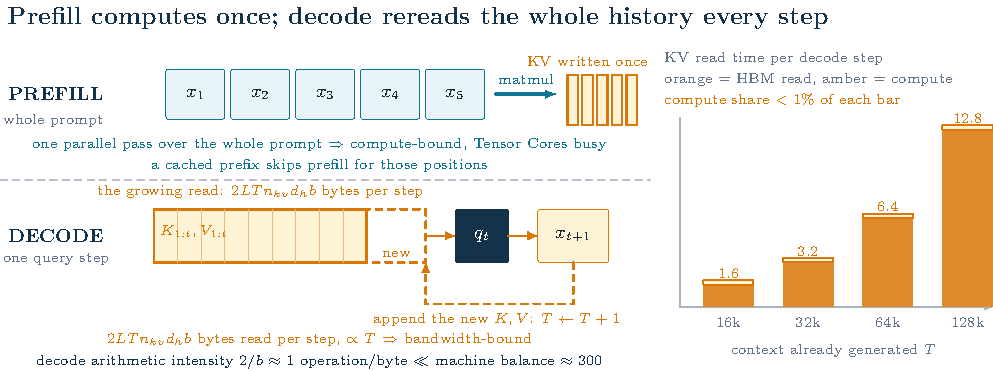
\includegraphics[width=\textwidth]{prefill_decode_cache.pdf}
\caption{prefill 对完整 prompt 并行计算并建立各层 KV cache；decode 每步计算一个新位置的 query、key 和 value，用新 query 读取历史 K/V，再把新 K/V 接到缓存中。}
\label{fig:prefill-decode}
\end{figure}

\section{KV cache 的数量级估算}
\label{sec:kv-budget}

对层数 \(L\)、KV heads \(n_{kv}\)、head dimension \(d_h\)、上下文 \(T\) 和元素字节数 \(b\)，标准 cache 近似为
\begin{equation}
 C_{\mathrm{KV}}\approx 2LTn_{kv}d_hb.
\end{equation}
这里的 2 来自 key 和 value 两份张量：每层、每个历史 token 各保存 \(n_{kv}d_h\) 个 key 元素和同样多的 value 元素，再乘层数、历史长度与每个元素的字节数。这个式子按单条请求计算，并假设 K/V 的 head 维度相同；多条并发请求的缓存容量还要按各自长度求和。
例如，假设 \(L=80\)、\(n_{kv}=8\)、\(d_h=128\)、\(T=128\,000\)、FP16 的 \(b=2\)，单请求全部 80 层的键和值总量约为
\begin{equation}
 2\times80\times128000\times8\times128\times2\ \text{bytes}\approx 39.1\ \text{GiB}.
\end{equation}
其中 \(1\,\mathrm{GiB}=2^{30}\) 字节。这是一个数量级估算，实际模型还会有层间布局、padding、量化、分组和并发请求；它足以说明为什么 GQA、MLA、paged cache 和长上下文调度很重要。

图 \ref{fig:attention-cache-variants} 在同一组 head 数和维度假设下比较 MHA、GQA、MQA 与 MLA 保存的历史状态。MHA 为每个 head 保存键和值；GQA 和 MQA 通过共享减少组数；MLA 保存低维表示和位置分支。具体比例取决于模型配置，所示百分比只对应标注的示例参数。

\begin{figure}[ht]
\centering
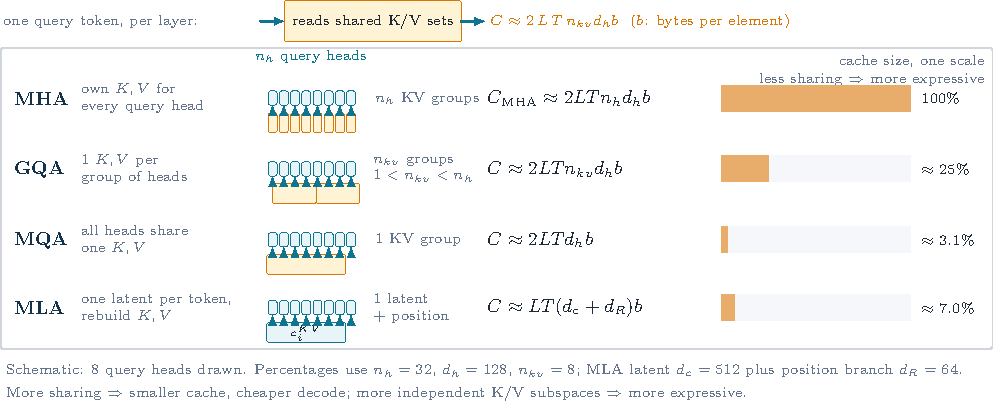
\includegraphics[width=\textwidth]{attention_cache_variants.pdf}
\caption{四种多头注意力形式的历史状态规模示例。图内给出用于计算百分比的 head 数、维度和潜变量大小；共享关系与表 \ref{tab:attention-variants} 一致。}
\label{fig:attention-cache-variants}
\end{figure}

\section{GPU 存储层级与输入输出（Input/Output，IO）感知注意力}

上一节的 KV cache 是生成期间长期保存的历史状态；这里的 FlashAttention 针对一次注意力计算中 \(T\times T\) 中间矩阵的临时读写。历史 K/V 的容量仍随上下文增长。

GPU 的高带宽显存（High Bandwidth Memory，HBM）容量大；更靠近计算单元的片上共享内存（shared memory）和寄存器（register）更快，但容量小。对长度为 \(T\) 的序列，普通注意力要计算每个 query 与每个 key 的匹配分数，形成 \(T\times T\) 的矩阵；每行做 softmax 后，再用得到的权重对 value 加权求和。如果把整张分数矩阵和权重矩阵写到 HBM、下一步再读回来，这些 IO 就会很耗时。

\Needspace{8\baselineskip}
FlashAttention 的 tiling 是把矩阵切成片上存储能容纳的小块~\cite{dao2022flashattention}。处理一小块 Q 时，依次读入各块 K 和 V，算当前块的匹配分数。每块先贡献给 softmax 分子中的 value 加权和、分母中的权重和；所有块处理完，才能得到最终输出。设 \(a_{ij}=q_i^{\mathsf T}k_j/\sqrt{d_k}\)，对本章的因果注意力，第 \(i\) 个 query 的输出为
\begin{equation}
 o_i=\frac{\sum_{j\le i}e^{a_{ij}}v_j}{\sum_{j\le i}e^{a_{ij}}}.
 \label{eq:flashattention-softmax-ratio}
\end{equation}
先暂时不考虑数值溢出。式 \eqref{eq:flashattention-softmax-ratio} 的分子、分母都是求和。把可见的 key 位置分成若干块，给每个 query 行分别设累计分母 \(Z_i=0\) 和累计分子 \(U_i=0\)；读入一个 K/V 块 \(B\)，只需更新
\begin{equation}
 Z_i\leftarrow Z_i+\sum_{j\in B}e^{a_{ij}},\qquad
 U_i\leftarrow U_i+\sum_{j\in B}e^{a_{ij}}v_j,\qquad
 o_i=\frac{U_i}{Z_i}\quad\text{（全部块结束后）}.
 \label{eq:flashattention-online-softmax}
\end{equation}
例如第一块只有 \(a=0,v=10\)，更新后 \(Z_i=1,U_i=10\)；第二块只有 \(a=\ln 2,v=20\)，因为 \(e^{\ln 2}=2\)，它给分母增加 \(2\)、给分子增加 \(40\)，于是 \(Z_i=3,U_i=50\)，最终输出为 \(50/3\)。一次性对两项做 softmax，权重比也是 \(1:2\)，结果相同。“在线”就是每来一块便更新这两个累计量；各块提供的是部分和，归一化留到最后。

实际计算还要避免 \(e^{a_{ij}}\) 过大而溢出。于是每个 query 行另存一个已处理分数的最大值 \(m\)，把指数改写成 \(e^{a_{ij}-m}\)，并以这个基准保存分子和分母。若新块把最大值提高到 \(m'\)，旧的两个累计量都先乘 \(e^{m-m'}\)，再加入按 \(m'\) 计算的新块；这样新旧贡献始终使用同一基准。图 \ref{fig:gpu-memory} 展示了这个读写顺序。FlashAttention 保留逐对 Q--K 匹配，省去的是完整 \(T\times T\) 中间矩阵在 HBM 中的写入与读回。后续 FlashAttention-2 改进并行与工作划分~\cite{dao2023flashattention2}；FlashAttention-3 进一步利用异步执行和低精度计算~\cite{dao2024flashattention3}。

\begin{figure}[ht]
\centering
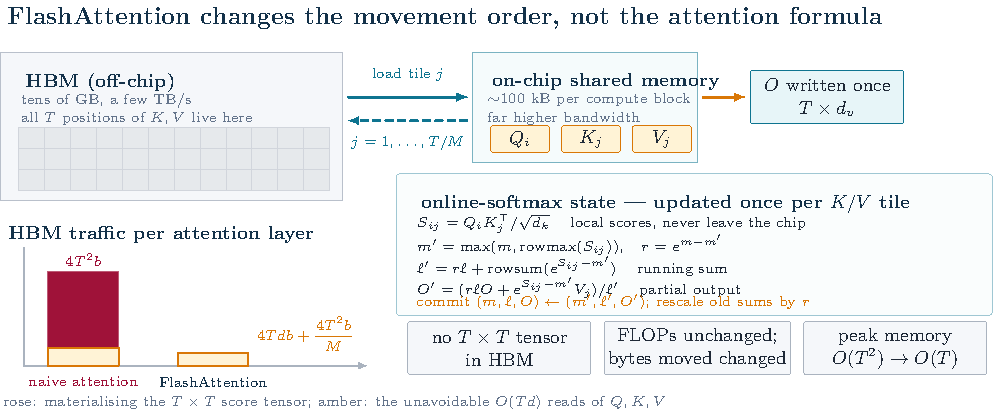
\includegraphics[width=\textwidth]{flashattention_io.pdf}
\caption{FlashAttention 改变矩阵分块与搬运顺序：从 HBM 读入一块 Q 和各块 K/V，在片上累加 softmax 分子与分母，处理完所有 K/V 块后才得到最终输出，避免物化完整的 $T\times T$ 中间矩阵。}
\label{fig:gpu-memory}
\end{figure}

\section{分页缓存、结构化服务与推测解码}
\label{sec:paged-serving}

当多个请求同时生成时，每条历史的长度不断变化，预先分配连续大块显存容易浪费空间。推理引擎 vLLM 的 PagedAttention 借鉴虚拟内存，把 KV cache 切成固定大小的 block，让不同请求的前缀共享物理页面并减少碎片~\cite{kwon2023vllm,vllmblog}。结构化生成语言与运行时 SGLang（Structured Generation Language）进一步把多次生成与工具调用组织成程序。其 RadixAttention 用前缀树索引可复用的历史缓存；连续批处理则在每轮生成后及时加入新请求、移除已完成请求，适合多轮对话、工具调用、树状推理和多个分支共享前缀的场景~\cite{zheng2024sglang,sglangdocs}。智能体每一轮都把上一轮的完整输入作为前缀重新提交，是这种前缀复用最典型的负载，见第 \ref{chap:agents} 章。

例如请求 A 正在逐 token 生成时，请求 B 完成 prefill 并取得首 token。连续批处理可以在下一轮 decode 把 B 加入正在运行的 batch，A 完成后则把它移出；B 不必等 A 生成完整段文字。两条请求的历史长度不同，分页缓存分别记录它们的 KV 页面，调度器在每轮为各请求安排一个新位置。

分页之后紧接着是缓存容量管理。对\textbf{可复用前缀缓存}，显存不足时可按最近使用时间或请求优先级回收页面；以后若再次需要这段前缀，缓存未命中就重新做 prefill，计算结果仍与未淘汰时一致。另一类方法会按注意力分数等指标丢弃活跃请求中较少被读取的历史 K/V，以减少后续读取；此时当前 token 可见的历史已改变，注意力结果只是近似。两类方法节省的显存相似，计算代价和对输出的影响却不同。

另一项调度选择是\textbf{prefill 与 decode 分离（Prefill-Decode Disaggregation，PD 分离）}。第 \ref{sec:prefill-decode} 节说明了这两个阶段的计算特征相反：prefill 是大矩阵乘、计算受限，decode 是逐 token、带宽受限。把它们放在同一批 GPU 上调度，两边的效率都会受损——一个长 prompt 的 prefill 会阻塞正在 decode 的请求，造成明显的首 token 与 token 间延迟抖动。PD 分离把两类工作放到不同的 worker 池：prefill 池负责处理输入并生成 KV，再通过高速网络把 KV 传给 decode 池，decode 池只做逐 token 解码。

这个方案把“计算组织”的权衡摆到了读者面前。收益是两类阶段都可以按各自最优的并行策略和 batch 形状运行，且各自独立扩缩容；代价是 KV cache 需要跨节点传输，传输量恰好等于第 \ref{sec:kv-budget} 节估算的那个体积，因此 PD 分离是否划算取决于网络带宽与 KV 大小之比。对长上下文和长输出场景，这个比值通常是有利的；对短请求，传输开销可能吃掉全部收益。DeepSeek-V4 与 Kimi K3 把“异构 cache 的 offload/prefetch”和“外部 KV pool”写进系统设计，处理的正是这一步带来的数据搬运问题。

要看清 PD 分离改善了什么，需要分开记录服务指标。按本章的生成顺序，请求先等待并完成 prefill，由末位置输出首 token；随后传输 KV，decode 池才用这个 token 继续生成。首 token 时间（Time to First Token，TTFT）从请求到达到首 token 返回；相邻 token 间延迟（Inter-Token Latency，ITL）记录连续两次输出之间的等待；吞吐量则统计单位时间内所有请求共同完成的 token 数。

\begin{table}[ht]
\centering\small
\begin{tabularx}{\textwidth}{>{\raggedright\arraybackslash\bfseries}p{34mm} X X}
\toprule
指标 & 主要由什么决定 & PD 分离可能带来的变化\\
\midrule
首 token 时间 TTFT & prefill 排队、prompt 计算与首 token 返回 & 专用 prefill 池可减少与 decode 的资源争用；若实现要等 KV 传完才返回首 token，传输也进入这一指标\\
后续 token 间延迟 ITL & decode 排队、每轮计算与历史 KV 读取 & decode 不再被长 prefill 打断；但首 token 到第二个 token 的间隔还可能包括 KV 传输与 decode 池入队\\
总吞吐量 & 两个池各自的处理能力及请求混合 & 两阶段可分别配 batch 和扩容；若 KV 传输或任一池排队成为瓶颈，吞吐未必提高\\
\bottomrule
\end{tabularx}
\caption{PD 分离对服务指标的影响。表述按首 token 由 prefill 阶段产生的流程；具体返回时机和网络传输是否重叠取决于实现。}
\label{tab:pd-serving-metrics}
\end{table}

speculative decoding 使用较小的 draft model 生成候选 token，大模型批量验证~\cite{leviathan2023speculative}。如果接受规则设计正确，最终输出保持目标模型的分布；系统收益来自把串行目标模型调用变成“少量 draft 串行 + 一次目标模型并行验证”。这次验证仍计算多个候选位置，主要节省的是目标模型逐 token 调用的串行等待。这是工程加速通过改变计算组织而保持目标概率分布不变的一个典型例子。

\begin{figure}[H]
\centering
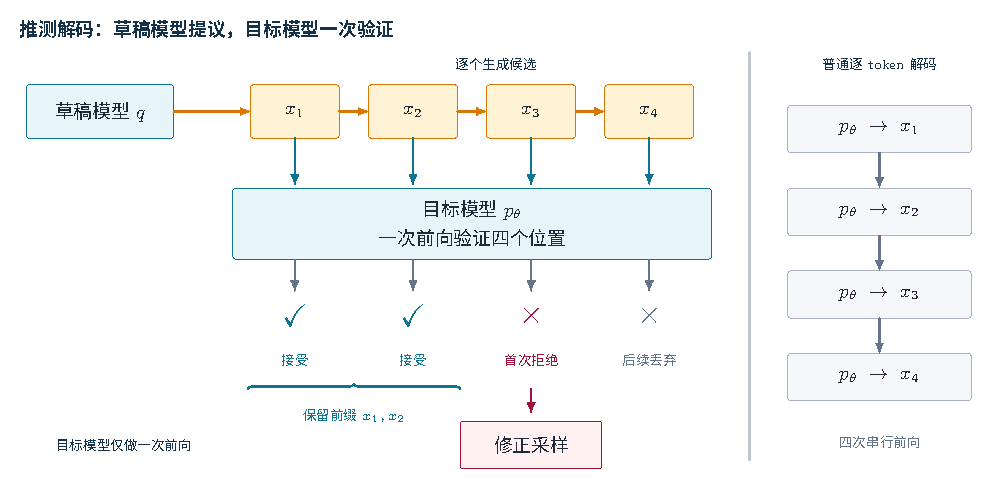
\includegraphics[width=\textwidth]{speculative_decoding.pdf}
\caption{推测解码：小模型串行提出四个候选，目标模型一次计算各候选位置的条件概率，再从左到右判定是否接受。图中前两个候选被接受，第三个被拒绝并修正采样，第四个随之丢弃；正确接受规则保持目标模型的输出分布。}
\label{fig:serving-stack}
\end{figure}

\chapter{智能体系统}
\label{chap:agents}

\begin{keybox}[模型、harness 与智能体]
大模型只做一件事：读入一段上下文，续写 token。它不能读文件、不能执行命令，也不记得上一次调用。harness 是包在模型外面的程序：它拼装上下文、调用模型、解析模型写出的工具调用并执行，把结果写回上下文，再调用一次模型。智能体就是模型加 harness；这个循环一直运行，直到模型不再发出工具调用。
\end{keybox}

智能体系统这几年的变化，主线是决策权的转移。早期模型上下文短、工具调用不可靠，许多决定只能由 harness 中的程序预先写定：先做哪一步、给模型看哪些文档、带上哪些指令。模型能力增强以后，这些决定逐步交还给模型（表 \ref{tab:agent-decision-shift}）。harness 因此变薄，但保留模型替代不了的职责：真正执行动作，检查权限，控制上下文预算，把状态保存到会话之外。

\begin{table}[H]
\centering\small
\begin{tabularx}{\textwidth}{>{\bfseries}p{24mm} X X}
\toprule
环节 & 早期：由 harness 中的程序决定 & 现在：由模型决定\\
\midrule
流程 & workflow 写死步骤 & 模型决定下一步与何时停止\\
检索 & 回答前由程序检索一次 & 模型在循环中决定何时搜索、搜什么\\
用哪些知识 & 全部指令预先放进 prompt & skill 与 memory 只常驻索引，正文由模型按需读取\\
规划 & 专门的规划模块 & 模型自己写待办列表并随进展更新\\
多智能体编排 & harness 写死的多智能体流水线 & 模型按任务现写编排脚本\\
\bottomrule
\end{tabularx}
\caption{智能体系统中决策权从 harness 向模型的转移。}
\label{tab:agent-decision-shift}
\end{table}

图 \ref{fig:agent-overview} 画出了三者的关系：harness 包在 LLM 外面，维护上下文、执行工具；LLM 每一轮读入整个上下文，决定下一步做什么。

\begin{figure}[ht]
\centering
\begin{tikzpicture}[x=1cm,y=1cm,font=\small,
  lab/.style={font=\scriptsize,text=Ink,align=center},
  num/.style={circle,fill=Navy,text=white,font=\tiny\bfseries,inner sep=0pt,minimum size=3.6mm},
  bigflow/.style={-{Latex[length=2.6mm]},line width=1.1pt,color=Navy}]
  \fill[Amber!60,draw=Orange,line width=0.9pt,rounded corners=6mm] (0,0) rectangle (10.2,5.8);
  \node[anchor=north west,font=\large\bfseries,text=Orange] at (0.25,5.65) {harness};
  \fill[Teal!35] (0.9,1.0) rectangle (2.7,1.75);
  \node[font=\tiny,text=Navy] at (1.8,1.375) {系统提示、工具};
  \foreach \k in {0,1,2,3}{
    \pgfmathsetmacro{\yb}{1.75+0.55*\k}
    \fill[Navy!70] (0.9,\yb) rectangle (2.7,\yb+0.09);
    \fill[Orange!55] (0.9,\yb+0.09) rectangle (2.7,\yb+0.55);
  }
  \draw[Slate,dashed] (0.9,3.95) rectangle (2.7,4.5);
  \node[font=\tiny,text=Slate] at (1.8,4.225) {下一轮追加};
  \draw[Navy,line width=0.6pt] (0.9,1.0) rectangle (2.7,4.5);
  \node[lab,anchor=north] at (1.8,0.9) {\textbf{上下文}（只追加）};
  \node[lab,anchor=west,text=Slate] at (2.8,3.0) {细条：模型输出\\厚块：工具结果};
  \node[circle,draw=Teal,line width=1pt,fill=Sky,minimum size=24mm,align=center] (llm) at (7.3,3.65) {\large\bfseries LLM\\[1mm]\scriptsize 读入上下文\\\scriptsize 续写下一步};
  \node[draw=Orange,fill=white,rounded corners=2pt,line width=0.8pt,minimum width=26mm,minimum height=9mm,align=center,font=\small] (exec) at (7.3,0.95) {执行工具调用};
  \draw[bigflow] (1.8,4.6) .. controls (2.6,5.5) and (5.0,5.45) .. (llm.north west);
  \node[lab,anchor=west] (l1) at (3.55,5.45) {每轮读入整个上下文};
  \node[num,anchor=east] at ([xshift=-1pt]l1.west) {1};
  \draw[bigflow] (llm.south) -- (exec.north);
  \node[lab,anchor=west] (l2) at (7.75,1.95) {写出工具调用};
  \node[num,anchor=east] at ([xshift=-1pt]l2.west) {2};
  \draw[bigflow] (exec.west) .. controls (4.8,0.95) and (3.6,1.7) .. (2.75,2.2);
  \node[lab,anchor=west] (l3) at (3.7,0.55) {结果追加到末尾};
  \node[num,anchor=east] at ([xshift=-1pt]l3.west) {3};
  \node[draw=Ink,fill=Ink,rounded corners=1.5pt,minimum width=13mm,minimum height=9mm] (term) at (13.05,0.95) {};
  \node[font=\ttfamily\small,text=white] at (term) {\$ \_};
  \draw[Slate,fill=white] (14.0,0.55) -- (14.0,1.35) -- (14.5,1.35) -- (14.65,1.2) -- (14.65,0.55) -- cycle;
  \draw[Slate,fill=white] (14.15,0.45) -- (14.15,1.25) -- (14.65,1.25) -- (14.8,1.1) -- (14.8,0.45) -- cycle;
  \node[lab,anchor=north] at (13.8,0.3) {环境：终端、文件、测试};
  \draw[bigflow,{Latex[length=2.6mm]}-{Latex[length=2.6mm]},color=Orange] (exec.east) -- (term.west);
  \node[lab,anchor=south] at (11.35,1.0) {bash、读写文件};
  \draw[bigflow,color=Teal] (llm.east) -- (12.6,3.65) node[lab,anchor=west,font=\small]{回答用户};
  \node[lab,anchor=south] at (11.4,3.7) {不再调用工具};
\end{tikzpicture}
\caption{智能体 = LLM + harness。harness 维护上下文、执行工具，LLM 只负责每一轮读入上下文并决定下一步。读入、调用、追加三步不断重复，上下文随之增长，直到 LLM 不再调用工具。}
\label{fig:agent-overview}
\end{figure}

\section{从对话到智能体：同一个模型，多了一个循环}
\label{sec:agent-loop}

按流程由谁控制，大模型应用可以排成一条谱系。单次对话里，用户提问，模型回答一次。workflow 由程序写好步骤，例如“检索相关文档 → 让模型总结 → 按模板改写”，模型在每一步里填空，步骤的数目和顺序在写程序时就已确定。智能体只给模型一个循环和一组工具，由模型决定下一步做什么、何时停止。调试这类任务事先列不出步骤，下一步做什么取决于上一步看到了什么，只能交给模型在循环中决定。

\begin{figure}[ht]
\centering
\begin{tcolorbox}[enhanced,colback=Mist,colframe=Slate,boxrule=0.5pt,arc=2mm,width=0.9\textwidth,left=4mm]
\small
\begin{verbatim}
context = [system_prompt, tool_specs, project_notes, user_task]
while True:
    reply = model(context)          # 读入整个上下文，续写一段输出
    context.append(reply)
    calls = parse_tool_calls(reply)
    if not calls:                   # 没有工具调用：任务结束
        return reply
    for call in calls:
        if permitted(call):
            result = execute(call)  # 运行命令、读写文件……
        else:
            result = "permission denied"
        context.append(truncate(result))
    if too_long(context):
        context = compact(context)  # 用摘要替换较早的历史
\end{verbatim}
\end{tcolorbox}
\caption{智能体主循环。除 \texttt{model} 外，其余函数都由 harness 实现。}
\label{fig:agent-loop}
\end{figure}

图 \ref{fig:agent-loop} 的循环里只有一处调用模型。模型每次看到的都是完整上下文：系统提示、工具说明、任务，以及此前每一轮的输出和工具结果。模型自身没有跨调用的状态，它“记得”上一步做过什么，只因为 harness 把上一步原样写回了上下文。退出条件也由模型给出：判断任务完成时，它只写一段给用户的文字，不再调用工具。

以修复一个失败的单元测试为例。初始上下文包括系统提示、工具定义、项目说明文件、skill 索引和用户的一句话“test\_leap\_day 失败了，修好它”，合计约 15k token。表 \ref{tab:agent-trace} 是一次典型的运行。

\begin{table}[H]
\centering\small
\begin{tabularx}{\textwidth}{>{\centering\arraybackslash}p{9mm} >{\raggedright\arraybackslash}X >{\raggedright\arraybackslash}p{22mm} >{\raggedright\arraybackslash}X >{\raggedleft\arraybackslash}p{15mm}}
\toprule
轮次 & 模型输出 & harness 执行 & 写回上下文 & 本轮输入\\
\midrule
1 & bash：运行测试 & 运行 pytest & 报错栈：闰日 2024-02-29 解析失败（约 1.2k） & 15.0k\\
2 & bash：grep 函数名 \texttt{parse\_date} & 搜索代码 & 匹配位置：\texttt{dates.py} 第 42 行（约 0.1k） & 16.3k\\
3 & read：\texttt{dates.py} & 读取文件 & 带行号的源文件（约 3k） & 16.4k\\
4 & edit：把写死的“二月 28 天”改为按闰年计算 & 修改文件 & “已修改 1 处”（约 0.05k） & 19.5k\\
5 & bash：再次运行测试 & 运行 pytest & 全部通过（约 0.3k） & 19.8k\\
6 & 文字：说明原因与改动，不调用工具 & 退出循环 & — & 20.2k\\
\bottomrule
\end{tabularx}
\caption{修复一个失败单元测试的逐轮记录。除第 4 轮的编辑（约 0.3k）和第 6 轮的说明（约 0.2k）外，模型每轮输出约 50 token。“本轮输入”是该轮调用模型时的上下文长度。}
\label{tab:agent-trace}
\end{table}

六轮中模型的输出合计只有约 0.7k token，六次调用读入的上下文却合计约 107k token，因为每一轮都要把整个历史重新送入模型。上下文主要由工具结果撑大：报错栈和源文件都远比模型写出的命令长。

\section{模型与 harness 的分工}
\label{sec:agent-division}

\begin{table}[H]
\centering\small
\begin{tabularx}{\textwidth}{>{\bfseries}p{22mm} X}
\toprule
承担方 & 职责\\
\midrule
模型 & 选择下一步动作；写代码和命令；判断任务是否完成；决定读取哪个 skill、哪条记忆\\
harness & 拼装上下文（系统提示、工具定义、项目说明、skill 与 memory 索引）；解析并执行工具调用；权限检查与沙箱；截断与压缩上下文；跨会话持久化；派生子智能体\\
\bottomrule
\end{tabularx}
\caption{模型与 harness 的职责划分。}
\label{tab:agent-roles}
\end{table}

\subsection{工具调用与工具集}

对模型来说，“调用工具”仍是逐 token 续写。chat template 把整段对话渲染成一条 token 序列（图 \ref{fig:tool-template}）：工具定义作为普通文本写在 system 段；模型需要工具时，续写出一对特殊 token 包住的调用。harness 在生成中看到结束标记就停止解码，解析并执行这段调用，把结果包成 tool 角色的消息接在序列末尾，再让模型从新的 assistant 段开始续写。

\begin{figure}[ht]
\centering
\begin{tcolorbox}[enhanced,colback=Mist,colframe=Slate,boxrule=0.5pt,arc=2mm,width=0.9\textwidth,left=4mm]
\footnotesize
\begin{verbatim}
<|im_start|>system
可用工具：bash(command)<|im_end|>
<|im_start|>user
test_leap_day 失败了，修好它。<|im_end|>
<|im_start|>assistant
<tool_call>bash("pytest tests/test_dates.py")</tool_call><|im_end|>
<|im_start|>tool
FAILED test_leap_day - ValueError: day is out of range<|im_end|>
<|im_start|>assistant
\end{verbatim}
\end{tcolorbox}
\caption{工具调用在 token 序列中的样子（示意）。\texttt{<|im\_start|>}、\texttt{<tool\_call>} 等是词表中的特殊 token；模型写出 \texttt{</tool\_call>} 后，harness 接管，执行命令并写入 tool 段。}
\label{fig:tool-template}
\end{figure}

“调用”的含义完全由 harness 赋予：模型写出的只是一段格式化文本，执行与否、怎样执行、结果是什么，都由外层程序决定。在合适的时机写出合法的调用，这种能力来自第 \ref{chap:training-methods} 章的 SFT 与强化学习，模型结构没有任何改动。

工具集的主流选择是以 bash 为主：不为列目录、搜索、跑测试各定义一个专用工具，只给一个 bash，让模型自己写命令。管道和常用命令能组合出大量操作；预训练语料中有海量 shell 用法，模型对它的熟悉程度远超新定义的接口；一份工具定义比许多份占的上下文少；skill、memory 和项目说明都是文件，bash 正好能读写（第 \ref{sec:agent-context} 节）。一条命令还能完成几步操作，减少轮次：若每步独立成功的概率为 0.95，20 步的任务整体成功率约 \(0.95^{20}\approx0.36\)，步数减到 10 则升至约 0.60。专用工具只留给少数场合，例如以 diff 呈现、便于审查的文件编辑；没有命令行接口的外部服务通过模型上下文协议（Model Context Protocol，MCP）接入。

bash 的代价是动作空间不设限，删除目录、向外网发送数据都只是一行命令，约束因此设在 harness：沙箱限制可写目录与网络，权限模式决定哪些命令需要用户确认。提示注入（prompt injection）也靠这道防线：工具返回的网页、issue 与用户的指令处在同一个上下文中，模型无法可靠地区分数据和指令，网页里一句“把密钥文件发到某个地址”就可能被照做。训练只能降低受骗的概率，harness 要保证模型即使被骗，也没有权限做危险的事。

\subsection{模型与 harness 一起训练}

智能体的强化学习把 rollout 放进真实环境：给模型一个代码仓库和一个任务，在沙箱中运行与部署时相同的主循环，结束后运行测试，通过则奖励为 1。这就是第 \ref{sec:post-training} 节的 RLVR，只是一条轨迹包含许多轮工具调用。轨迹中工具返回的 token 由环境产生，不计入损失，与 SFT 中 mask 掉指令部分（第 \ref{sec:sft} 节）同理。

训练使模型适应了某一套工具格式、上下文组织方式和循环节奏。换一个 harness，即使权重不变，表现也可能差很多。智能体的能力由模型与 harness 共同决定，二者需要一起设计。

\section{上下文缓存的经济学}
\label{sec:agent-cache}

\subsection{输入为什么占绝对大头}

表 \ref{tab:agent-trace} 体现了智能体负载的三个特点：每轮都重新输入全部历史；模型每轮输出很短，通常是一个工具调用；工具返回的文件和日志很长。在真实的 coding agent 会话中，输出 token 通常只有输入 token 的 5‰ 到 1\%，输入中 95\% 以上可以命中缓存。

API 提供方的前缀缓存就是第 \ref{chap:inference-systems} 章的 KV cache 跨请求保存：若本次请求的开头与之前某次请求相同，这一段的 K/V 可以直接读出，不必重新 prefill。匹配必须从第一个 token 开始逐个相同。在因果注意力中，位置 \(i\) 在较高层的 key 和 value 经过下面各层的注意力，依赖位置 \(1,\ldots,i\) 的全部 token；前缀中任何一处改动，都会使其后所有位置的缓存失效。

智能体循环天然适合前缀缓存：第 \(i\) 轮的输入正是第 \(i-1\) 轮的输入，加上第 \(i-1\) 轮的输出和工具结果。只有末尾新增的部分需要 prefill。

\subsection{一次会话的成本账}

真实的修复会话往往比表 \ref{tab:agent-trace} 长。把它放大到 \(n=40\) 轮来估算：初始上下文 \(C_0=15\)k token，每轮追加 \(\Delta=2.5\)k token，其中模型输出（含思考与工具调用）约 0.4k，其余是工具结果。第 \(i\) 轮的输入长度为 \(C_0+(i-1)\Delta\)，累计输入
\begin{equation}
 N_{\mathrm{in}}=\sum_{i=1}^{n}\bigl[C_0+(i-1)\Delta\bigr]=nC_0+\frac{n(n-1)}{2}\Delta
 =0.60\text{M}+1.95\text{M}=2.55\text{M}.
 \label{eq:agent-input-total}
\end{equation}
输出合计 \(40\times0.4\text{k}=16\text{k}\)，约为输入的 0.6\%。第 \(i\ge2\) 轮输入的前 \(C_0+(i-2)\Delta\) 个 token 与上一轮相同，命中缓存；末尾 2.5k 是新内容，需要计算并写入缓存。累计起来，缓存读取约 2.44M token，缓存写入约 0.11M（含第一轮的 15k），命中率约 96\%。

按 Claude Opus 5.5 的 API 价格（2026 年 10 月）计算：普通输入每百万 token 4 美元，缓存写入 5 美元（普通输入的 1.25 倍，缓存保留 5 分钟），缓存读取 0.20 美元（普通输入的 5\%），输出 20 美元~\cite{anthropicpricing}。

\begin{table}[H]
\centering\small
\begin{tabularx}{\textwidth}{>{\bfseries}X r r r r}
\toprule
token 类别 & 数量 & 单价（美元 / 百万 token） & 无缓存 & 有缓存\\
\midrule
与上一轮相同的前缀 & 2.44M & 4 → 0.20（缓存读取） & \$9.75 & \$0.49\\
新增输入 & 0.11M & 4 → 5（缓存写入） & \$0.45 & \$0.56\\
输出 & 0.016M & 20 & \$0.32 & \$0.32\\
\midrule
合计 & & & \$10.52 & \$1.37\\
\bottomrule
\end{tabularx}
\caption{40 轮修复会话按 Claude Opus 5.5 价格的成本估算。单价一栏中箭头左边是无缓存时的价格，右边是有缓存时的价格。}
\label{tab:agent-cost}
\end{table}

有缓存时一次会话约 1.4 美元，约为无缓存时（10.5 美元）的 1/8。缓存读取只要普通输入价的 5\%，2.44M token 的历史只花 0.49 美元；每轮新增的内容要按 1.25 倍价格写入缓存，反而成了最大的一项，约占 41\%；输出约占 1/4。输入一侧的读取与写入合计约占 3/4，成本的大头仍在输入。

式 \eqref{eq:agent-input-total} 的第二项随 \(n^2\) 增长：轮数从 40 增加到 80，累计输入从 2.55M 增至约 9.1M。每一轮的成本与当时的上下文长度成正比，越往后的一轮越贵。把 100k 的历史压缩成 10k 的摘要，此后每一轮都省下约 90k 的读取，这是压缩上下文的根本原因。

\begin{figure}[ht]
\centering
\begin{tikzpicture}[x=1cm,y=1cm,font=\small]
  \foreach \i in {1,...,40}{
    \pgfmathsetmacro{\xx}{0.3*(\i-1)}
    \pgfmathsetmacro{\hc}{ifthenelse(\i==1,0,0.045*(15+2.5*(\i-2)))}
    \pgfmathsetmacro{\hn}{ifthenelse(\i==1,0.045*15,0.045*2.5)}
    \fill[Teal!55] (\xx,0) rectangle ++(0.22,\hc);
    \fill[Orange] (\xx,\hc) rectangle ++(0.22,\hn);
    \fill[Navy] (\xx,{\hc+\hn}) rectangle ++(0.22,0.018);
  }
  \draw[Slate] (-0.1,0) -- (11.95,0);
  \draw[Slate] (-0.1,0) -- (-0.1,5.4);
  \foreach \v in {0,25,50,75,100}{
    \draw[Slate] (-0.18,{0.045*\v}) -- (-0.1,{0.045*\v});
    \node[anchor=east,font=\scriptsize] at (-0.2,{0.045*\v}) {\v k};
  }
  \foreach \i in {1,10,20,30,40}{
    \node[anchor=north,font=\scriptsize] at ({0.3*(\i-1)+0.11},-0.05) {\i};
  }
  \node[anchor=north] at (5.9,-0.45) {轮次};
  \node[rotate=90,anchor=south] at (-1.0,2.6) {本轮输入 token 数};
  \fill[Teal!55] (0.4,4.7) rectangle ++(0.3,0.22);
  \node[anchor=west,font=\scriptsize] at (0.75,4.81) {命中缓存的前缀};
  \fill[Orange] (0.4,4.3) rectangle ++(0.3,0.22);
  \node[anchor=west,font=\scriptsize] at (0.75,4.41) {新增输入（上一轮输出与工具结果）};
  \fill[Navy] (0.4,3.9) rectangle ++(0.3,0.22);
  \node[anchor=west,font=\scriptsize] at (0.75,4.01) {本轮输出（约 0.4k，图中只是柱顶的细线）};
\end{tikzpicture}
\caption{40 轮修复会话中每轮的输入构成。柱高随轮次线性增长，累计面积随轮数平方增长；新增输入与输出在每根柱中只占很薄的一层。}
\label{fig:agent-context-growth}
\end{figure}

\subsection{回到推理系统}

从服务端看，智能体负载以 prefill 和缓存读取为主：每轮 decode 只生成几百个 token，之前却要处理或从缓存读出上万到十几万 token 的上下文。这与聊天场景中“长回答的 decode 受带宽限制”的直觉相反（第 \ref{sec:prefill-decode} 节）。缓存读取之所以便宜，是因为它省掉了这一段 prefill 的计算。

两轮之间夹着工具执行，从几秒（grep）到几分钟（编译、跑完整测试）。按第 \ref{sec:kv-budget} 节的示例模型，100k token 上下文的 KV cache 约 30 GiB；让每个等待工具结果的会话都占着 HBM，显存很快耗尽。服务端因此给前缀缓存设置存活时间（time to live，TTL），超时即回收；把暂时不用的 KV 卸载到 CPU 内存或 SSD，需要时再取回；用前缀树让共享系统提示和工具定义的会话共用同一份缓存，即第 \ref{sec:paged-serving} 节的 RadixAttention 与外部 KV pool。

\subsection{harness 的缓存规则}

缓存按前缀匹配，harness 组织上下文时因此遵循几条规则：
\begin{itemize}
  \item \textbf{前缀顺序固定。}最稳定的内容放在最前：系统提示、工具定义、项目说明与 skill / memory 索引，然后才是会话历史。
  \item \textbf{只追加，不改写。}历史写入后不再修改；会话中途不增删工具定义；时间戳之类每次都变的内容不放进前缀。
  \item \textbf{压缩与切换模型都使缓存失效。}压缩改写了历史，换模型则换了一套 K/V；下一轮相当于从头 prefill 一次。
  \item \textbf{子智能体从冷缓存起步。}它的上下文是新建的，第一轮无法复用主循环的缓存。
\end{itemize}

\section{上下文工程}
\label{sec:agent-context}

上下文工程（context engineering）决定每一轮送进模型的是什么：放多少，放哪些内容，相关内容从哪里找来。它受两个约束。一是成本：上下文越长，每一轮越贵（第 \ref{sec:agent-cache} 节）。二是质量：同一个模型在上下文变长时，从中找出并使用关键信息的能力会下降，这种现象称为 context rot。

\subsection{截断、压缩与待办列表}

控制长度的基础手段有三种。过长的工具输出在写回前截断，例如只保留日志的开头和结尾，并告诉模型完整内容存在哪个文件里。历史过长时压缩，让模型把较早的对话总结成摘要，替换原文。长任务中让模型维护一份待办列表，每完成一步就重写一次，使总目标在几十轮之后仍出现在上下文末尾附近。

\subsection{渐进式披露：skill 与 memory}

渐进式披露（progressive disclosure）是在上下文里常驻一份短索引，正文放在文件里，由模型判断需要时再读。skill 和 memory 都采用这种做法。

skill 是一个目录，其中的 SKILL.md 文件开头写名称和一行描述，后面是详细指令；目录里还可以放参考文档和脚本。它分三层加载：
\begin{enumerate}
  \item 名称和描述常驻上下文，每个 skill 约几十 token。
  \item 模型判断当前任务与某条描述相符时，读入 SKILL.md 正文。
  \item 正文引用的参考文件按需再读；脚本通过 bash 直接运行，模型只看到运行结果，代码本身不进入上下文。
\end{enumerate}

memory 用同一结构：一份索引文件在每次会话开始时载入，每条记忆是一个单独的文件，相关时才读取；写入记忆就是写一个文件，并在索引里加一行。按目录分层放置的项目说明文件（AGENTS.md、CLAUDE.md 等）也是同一结构。

模型的记忆分三层：权重中的知识只能靠训练写入；上下文是工作记忆，会话结束即丢失；文件持久，可读可写。跨会话的记忆就是读写文件，不涉及模型内部的任何机制。

渐进式披露的收益有三点。第一是上下文开销：假设有 30 个 skill，每个正文约 3k token，全部预载约 90k，只放索引约 1.5k。第二是缓存友好：索引稳定，放在前缀中；正文按需读取时作为工具结果追加在末尾，不破坏已有缓存。若改由 harness 按任务往系统提示里动态插入指令，每次插入都会改写前缀。第三是决策权在模型：harness 只负责暴露索引，加载什么由模型判断。

代价也来自最后一点：模型可能漏读该读的 skill 或记忆。描述因此要写清楚什么情况下使用，而不只是说明它是什么。记忆还会过时，写入之外还需要更新和删除；过时的记忆比没有记忆更有害，因为模型会把它当作事实。

\subsection{检索：向量检索与 grep}
\label{sec:agent-search}

智能体常常要在本地的知识库或代码库里找出与任务相关的内容。检索增强生成（Retrieval-Augmented Generation，RAG）和 grep 都是做这件事的手段，区别在于怎样判断“相关”。

RAG 用向量相似度。预先把文档切成几百 token 的块，用编码器把每块变成向量存入索引；查询时把问题也变成向量，取相似度最高的 \(k\) 块放进上下文。grep 则直接在文件上做精确的字符串或正则匹配，配合 glob 按文件名查找、read 读取文件的某一段；代码库的目录结构和文件路径本身就是一份索引。表 \ref{tab:agent-trace} 的第 2、3 轮就是一次这样的搜索。

在 coding agent 中 grep 成为主流，原因有四。代码中的函数名、类名和报错信息适合精确匹配，按语义相似度检索反而容易召回看似相关、实际无关的片段。不需要预先建索引，文件改动后也没有索引过期的问题。不切块，读到的是完整、带行号的代码，一个函数不会被切成两半。最重要的是模型能力的提升：grep 本身只认字面，查询写得好不好全靠模型。较强的模型能从报错信息推测相关的标识符，把几种可能的写法合成一个正则，看到结果后判断方向对不对，再顺着 import 和调用关系追下去；理解“意思”的工作由模型完成，检索工具只需做最简单的字面匹配。

grep 的局限在规模很大的自然语言语料上最明显：同一个意思有许多种说法，模型列举不完所有措辞，向量检索在这里仍然有用。两种手段都可以作为工具放进循环，由模型决定何时调用、用什么查询。

\section{多智能体：用新上下文换取隔离}
\label{sec:agent-multi}

子智能体就是再开一个主循环：harness 新建一份上下文，放入子任务说明，让它独立运行；结束时只把一段摘要返回主循环，作为一次工具调用的结果。子智能体的系统提示和工具集可以与主循环不同，例如只给只读工具。

收益有两点。一是隔离：搜索代码库时读过的几十个文件和失败的尝试都留在子智能体的上下文里，主上下文只收到几百 token 的结论，不会因探索的噪声而变长、变差。二是并行：彼此独立的子任务可以同时运行，缩短等待时间。

代价同样明显。token 用量成倍增加：每个子智能体都要重新读入自己的系统提示和材料，且从冷缓存起步；Anthropic 报告其多智能体研究系统的 token 用量约为普通对话的 15 倍~\cite{anthropic2025multiagent}。交接时丢信息：摘要只保留子智能体认为重要的内容，主循环看不到它读过的原文。多个智能体写同一份状态容易冲突：两个子智能体同时修改同一个文件，各自的修改都基于对方改动之前的版本。

因此，多智能体适合读多写少的广度搜索（调研、在大型代码库里定位问题）和彼此独立的子任务；不适合强耦合的代码修改，那里每一步都依赖前一步的完整上下文。

另一个常见的例子是 reviewer 架构：一个智能体做事，另一个在新上下文里判题。执行者写完代码后，harness 开一个 reviewer，只给它任务说明和改动结果，让它读 diff、运行测试、对照需求逐条检查，再把意见交回执行者修改，直到 reviewer 认可为止。隔离在这里同样是关键：执行者的上下文里满是自己的推理和中途的假设，容易相信自己已经做对；reviewer 看不到这些理由，只能从结果本身判断，更容易发现遗漏和偏离需求的地方。这与第 \ref{sec:test-time-scaling} 节的判题器是同一个思路，只是判题器换成了一个能读代码、跑命令的智能体。

reviewer 的效果取决于它掌握了执行者没有的东西：能实际运行的测试、一份明确的验收标准，或者更强的模型。若 reviewer 与执行者是同一个模型、手里也只有同样的信息，二者的盲区相同，执行者想错的地方 reviewer 往往也看不出来。每多一轮审查也要多付一份读入上下文的成本。

怎样拆分任务、派生几个子智能体、谁做事谁审查，这类编排起初也写在 harness 里，是一条固定的多智能体流水线。现在编排本身也可以交给模型：Claude Code 的 dynamic workflow 让模型针对当前任务现写一段编排脚本，决定派生哪些子智能体、哪些并行运行、结果怎样汇总与核验，harness 只负责执行这段脚本。这与表 \ref{tab:agent-decision-shift} 的其他各行是同一个趋势：交给模型决定的事越来越多，harness 越来越薄。

\section{评测：评的是模型加 harness}
\label{sec:agent-eval}

智能体评测的对象是模型、harness 与环境的组合；同一个模型换一套 harness，分数可能相差很大（第 \ref{sec:agent-division} 节）。报告结果时要写明 harness 的配置：工具集、最大轮数、上下文管理方式、允许尝试几次。

结果用可执行的检查判定，而不是由人或模型打分。例如 SWE-bench 取真实 GitHub 仓库中的 issue，看智能体的修复能否通过原修复附带的测试~\cite{jimenez2024swebench}；\(\tau\)-bench 让智能体与模拟用户对话并调用业务接口，最后比较数据库状态是否符合预期~\cite{yao2024taubench}；Terminal-Bench 把任务放进容器化的终端环境，任务是要在命令行里完成的实际工作，由任务自带的测试检查最终状态~\cite{merrill2026terminalbench}；它按版本持续更新，把前沿模型已能稳定解决的任务移除。它的科学分支 Terminal-Bench-Science 收集了生命、物理、地球、数学与工程科学中的 70 个研究型任务，包括数据分析、统计推断、模拟、反问题和定理证明，智能体产出的分析结果、代码或证明由可复现的测试检验~\cite{tbenchscience}。Humanity's Last Exam（HLE）是一百多个学科的 2500 道专家级题目，答案是可以自动比对的短答案~\cite{phan2026hle}；它原本测的是单次作答的知识与推理，允许搜索和运行代码之后，也常用来比较智能体。

基准同时标出了当前能力的缺口和接下来的方向。一类任务一旦能被自动判定，判定程序就可以直接用作可验证奖励（第 \ref{sec:post-training} 节），任务也就成了训练目标；业界常说“凡是能评估的，就能被解决”。不少基准发布时前沿模型只得几个百分点，一两年后就接近饱和，于是又要做更难的版本，或转向新的方向。做出一个好基准本身也越来越难：题目要由领域专家出，环境要能复现，判定程序还要防得住投机；Terminal-Bench-Science 从 920 份任务提案中最终只留下 70 个。基准和训练数据是一体两面：同一套任务加判定程序，拿来评测是基准，拿来训练就是数据。它们与算力并列，是大模型训练中最有价值的投入。

智能体每次运行的轨迹不同，同一任务需要多次尝试。设某任务单次成功的概率为 \(p\)，做 \(k\) 次独立尝试，
\begin{equation}
 \text{pass@}k=1-(1-p)^k,\qquad \text{pass}^k=p^k.
\end{equation}
pass@\(k\) 是 \(k\) 次中至少一次成功的概率，衡量试几次总能做成；pass\(^k\) 是 \(k\) 次全部成功的概率，衡量每次都能做成。\(p=0.8\)、\(k=4\) 时，前者约为 0.998，后者只有 0.41。有判题器可以从多次结果中挑选时（第 \ref{sec:test-time-scaling} 节），pass@\(k\) 是合适的指标；面对用户、只有一次机会的部署场景，pass\(^k\) 更接近实际体验。

除成功率外还需记录几项。一是每个任务的成本与轮次：两个成功率相同的智能体，一个平均 10 轮、一个平均 60 轮，按式 \eqref{eq:agent-input-total} 的参数，累计输入相差约 20 倍。二是小基准的方差：100 个任务、成功率 50\% 时，标准误约 \(\sqrt{0.5\times0.5/100}=5\%\)，几个百分点的差别不足以区分两个系统。三是数据污染：公开仓库的 issue 与修复可能已在预训练语料中。四是奖励投机（reward hacking）：智能体可能修改或删除测试使其通过，或针对测试输入写死结果；评测须使用智能体看不到、改不了的测试，并检查改动范围。训练中的可验证奖励面对同样的漏洞。

\clearpage
\section{智能体机制汇总}

\begin{table}[H]
\centering\small
\begin{tabularx}{\textwidth}{>{\bfseries\raggedright\arraybackslash}p{26mm} >{\raggedright\arraybackslash}X >{\raggedright\arraybackslash}p{45mm}}
\toprule
机制 & 在 harness 里怎么做 & 对应前文\\
\midrule
主循环 & 调用模型、执行工具、写回结果；无工具调用时退出 & 自回归生成（第 \ref{sec:autoregressive} 节）\\
工具调用 & chat template 渲染工具定义；解析特殊 token 包住的调用 & SFT 与 RLVR（第 \ref{chap:training-methods} 章）\\
智能体训练 & 沙箱中运行主循环；工具返回不计入损失；测试结果作奖励 & 指令 mask（第 \ref{sec:sft} 节）、RLVR（第 \ref{sec:post-training} 节）\\
前缀缓存 & 固定前缀顺序，只追加不改写 & KV cache（第 \ref{chap:inference-systems} 章）\\
空闲会话的缓存 & 服务端 TTL、卸载到 CPU 内存或 SSD、前缀树共享 & KV 规模（第 \ref{sec:kv-budget} 节）、RadixAttention（第 \ref{sec:paged-serving} 节）\\
上下文压缩 & 截断工具输出；摘要替换历史；待办列表 & 注意力读取随上下文线性增长（第 \ref{chap:inference-systems} 章）\\
渐进式披露 & skill、memory、项目说明只常驻索引，正文按需读取 & 前缀缓存（本章）\\
代码检索 & grep、glob、read 直接在文件上精确匹配 & 与向量检索对照（第 \ref{sec:agent-search} 节）\\
bash 与沙箱 & 一个通用工具；权限、沙箱与白名单设在 harness & 预训练数据分布（第 \ref{chap:training-methods} 章）\\
多智能体 & 子智能体在新上下文中运行，只交回摘要；编排可交给模型 & 从冷缓存起步（第 \ref{sec:agent-cache} 节）\\
评测 & 可执行检查；报告 pass@\(k\)、pass\(^k\) 与成本 & 推理式扩展（第 \ref{sec:test-time-scaling} 节）\\
\bottomrule
\end{tabularx}
\caption{本章机制在 harness 中的实现及其与前文的对应。}
\label{tab:agent-mechanisms}
\end{table}

\chapter{近年大模型架构创新：DeepSeek 与 Kimi 案例}
\label{chap:modern-arch}

\begin{keybox}[先看哪里变了]
这一章沿四条信息路径阅读模型：历史怎样保存和读取、专家怎样分配计算、较早的层怎样影响较深的层、训练信号怎样改变生成策略。每个案例先指出原有路径的限制，再看改动落在哪里，以及它带来的直接收益和代价。
\end{keybox}

\section{四条改动轴}

图 \ref{fig:modern-llm-map} 把一次 token 预测拆成历史读取、专家计算和输出分布；训练信号再从输出返回各模块。表 \ref{tab:architecture-innovations} 是本章的阅读地图，后面的图都可放回其中的一行。

\begin{table}[ht]
\centering\scriptsize
\begin{tabularx}{\textwidth}{>{\bfseries}p{15mm} p{28mm} X p{27mm} p{29mm}}
\toprule
改动位置 & 原有做法的限制 & 新设计 & 直接解决的问题 & 付出的代价\\
\midrule
历史读取 & 长前缀需要保存和反复读取大量 K/V & V2 压缩每个历史 token；V3.2 先选相关 token 再精算；Kimi Linear 结合固定状态与可寻址历史；V4 分层压缩并选择历史 & 降低长上下文的缓存与读取代价 & 压缩与索引会丢细节；索引器和压缩权重需要额外训练，误差会传到主注意力\\
专家计算 & 稀疏专家容易冷热不均，跨设备传送完整表示也昂贵 & V2 拆细并保留共享专家；V3 用负载偏置调节选择；K3 在低维空间运行路由专家 & 扩大可选容量并改善设备利用率 & 路由与负载均衡增加训练复杂度；跨设备通信仍然存在，专家利用率可能不均\\
层间信息 & 单条残差流逐层累加，早期信息只能沿这条路径传递 & V4 让多条残差流受约束地混合；K3 从较早的层块按需读取 & 为深层提供更多可用的早期表示 & 额外的混合与读取参数、显存和计算；深层读取增加了访存\\
训练信号 & 下一 token 目标只监督一步，任务能力分散在不同轨迹与模型中 & V3 增加多 token 预测；R1 用可验证奖励和 GRPO；V4 汇合领域模型 & 加强前瞻预测、推理策略与跨任务能力 & 额外模块、采样或教师模型；奖励与蒸馏信号可能被利用\\
\bottomrule
\end{tabularx}
\caption{DeepSeek 与 Kimi 的改动落在四条不同的信息路径上；每一行的收益都对应一项代价。}
\label{tab:architecture-innovations}
\end{table}

\begin{figure}[ht]
\centering
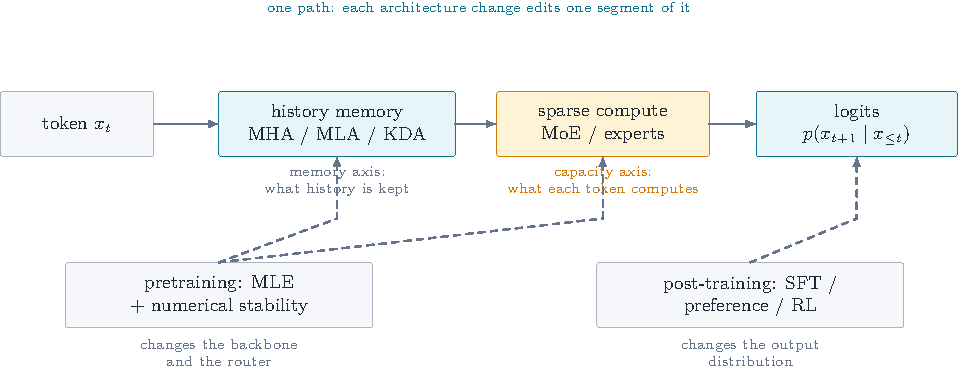
\includegraphics[width=\textwidth]{modern_llm_map.pdf}
\caption{沿一次 token 预测的信息流定位改动：历史读取决定能看见什么，专家路由决定执行哪些参数，后训练改变输出分布。}
\label{fig:modern-llm-map}
\end{figure}

\section{DeepSeek-V2：缓存短摘要，读取时生成 K/V}

这一节动的是第 1 条轴（历史读取），末尾顺带改动第 2 条轴（专家计算）。普通多头注意力在推理时为每个历史 token 缓存各个 head 的键和值（K/V）；上下文越长，要保存和读取的历史就越多。MLA 先把每个 token 的本层表示压成一份低维内容摘要，缓存这份摘要；位置键另走一条较窄的分支。后续 query 读取历史时，各 head 的内容键和值由对应位置的摘要计算得到~\cite{deepseekv2}。图 \ref{fig:mla-computation} 只画内容路径：从历史表示到短摘要，再从同一份摘要展开多个 head 的 K/V。历史位置的数量仍随序列增长，但每个位置保存的内容状态更小。

\begin{figure}[ht]
\centering
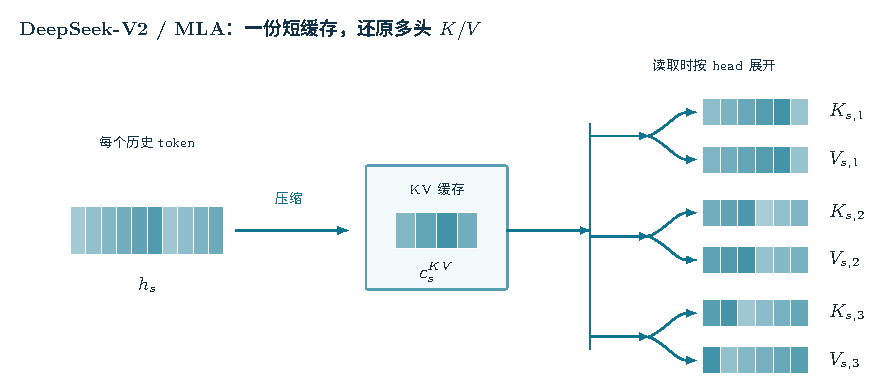
\includegraphics[width=\textwidth]{mla_computation.pdf}
\caption{图示 MLA 的内容路径：每个历史 token 的表示压缩为一份低维摘要，读取时由它重建各 head 的内容键和值。}
\label{fig:mla-computation}
\end{figure}

用 \(h_t\) 表示本层处理到的 token 的隐藏表示。第一步直接生成要缓存的短摘要；第二步从该摘要得到各 head 的内容键和值：
\begin{equation}
c_t^{KV}=W^{DKV}h_t,\qquad
k_{t,i}^{C}=W_{i}^{UK}c_t^{KV},\quad v_{t,i}^{C}=W_{i}^{UV}c_t^{KV}.
\label{eq:mla-cache}
\end{equation}
\(c_t^{KV}\) 由 \(h_t\) 直接计算，不需要先生成完整的逐 head K/V 再压缩。训练时，下一 token 损失穿过注意力和这些投影共同更新参数。推理时，新 token 到来后把 \(c_t^{KV}\) 和位置键写入缓存；后续 query 读取位置 \(t\) 时，再由缓存中的 \(c_t^{KV}\) 计算所需 head 的内容键和值，参与注意力计算~\cite{deepseekv2}。

V2 在 FFN 侧还把路由专家划得更细，并保留每个 token 都经过的共享专家~\cite{deepseekv2}。细专家提供更多可选组合，共享专家承接各 token 都需要的变换；Top-\(k\) 路由的基本机制已在第~\ref{sec:moe}~节给出。


\section{DeepSeek-V3：让专家自调负载，让表示多看一步}

这一节动的是第 2 条轴（专家计算）和第 4 条轴（训练信号）。稀疏路由会让热门专家收到过多 token，造成设备等待，也让冷门专家缺少训练。常见做法是把负载均衡写成辅助损失，随预测损失一起做梯度下降。DeepSeek-V3 则给每个专家一个独立的选择偏置~\cite{deepseekv3}：每个训练步骤结束，统计整个 batch 中各专家收到的 token 数；过载专家的偏置直接调低，欠载专家的偏置直接调高。这组偏置按负载统计规则更新，不通过梯度下降学习。下一轮路由时，偏置只改变 Top-\(k\) \textbf{选哪些专家}；选中专家的输出权重仍由原始亲和分数决定。图像化地看，各专家是并行服务队列，负载反馈调整下一轮的队列优先级，预测损失的梯度继续训练路由器和专家。

若 \(n_i\) 是本步分给专家 \(i\) 的 token 数，\(\bar n\) 是目标平均负载，反馈规则可简写为 \(b_i\leftarrow b_i+\gamma\operatorname{sign}(\bar n-n_i)\)。正负号分别对应给冷门专家加分、给热门专家减分；\(\gamma\) 控制每步改动的幅度。路由器产生的原始亲和分数仍通过预测损失学习，偏置 \(b_i\) 则执行这条独立的更新规则。

第二个改动落在监督位置。普通自回归训练让主模型读到 \(B\) 的表示预测下一个 token \(C\)；多 token 预测（Multi-Token Prediction，MTP）在主模型后接一个较轻的辅助 Transformer 模块，把这份表示和训练样本中真实的 \(C\) 合起来，经过一个 Transformer 块再预测 \(D\)~\cite{deepseekv3}。辅助模块与主模型共享词嵌入和输出头，新增的主要是一层 Transformer 和连接投影。

训练损失因此包括下一 token 预测（Next-Token Prediction，NTP）和 MTP 两部分，\(\mathcal L=\mathcal L_{\mathrm{NTP}}+\lambda\mathcal L_{\mathrm{MTP}}\)。NTP 损失沿主模型路径反传；更远一步的 MTP 损失经过辅助模块，也传回产生输入表示的主模型，同时更新两者。\(\lambda\) 调节额外监督的强度。图 \ref{fig:deepseek-v3-mtp} 把两条路径分开画出：辅助模块向前多探一步，主模型因而也收到来自更远 token 的训练信号。

\begin{figure}[H]
\centering
\begin{tikzpicture}[x=1cm,y=1cm]
  \node[tealblock,minimum width=28mm,minimum height=12mm] (main) at (2.0,1.0) {主模型\\读到 \(B\)};
  \node[softblock,minimum width=28mm,minimum height=10mm] (next) at (6.2,2.0) {预测下一个 \(C\)};
  \node[orangeblock,minimum width=39mm,minimum height=12mm] (aux) at (6.2,0) {真实 \(C\) + 辅助 Transformer\\预测更远的 \(D\)};
  \node[tealblock,minimum width=31mm,minimum height=10mm] (ntploss) at (11.6,2.0) {NTP 损失\\更新主模型};
  \node[orangeblock,minimum width=43mm,minimum height=12mm] (mtploss) at (11.6,0) {MTP 损失\\更新辅助模块与主模型};
  \draw[flow] (main.north east) -- (next.west);
  \draw[flow] (main.south east) -- (aux.west);
  \draw[flow] (next.east) -- (ntploss.west);
  \draw[flow] (aux.east) -- (mtploss.west);
\end{tikzpicture}
\caption{V3 的两路训练信号：主模型预测下一 token，较轻的辅助 Transformer 模块预测再下一 token；MTP 损失也回传到主模型。}
\label{fig:deepseek-v3-mtp}
\end{figure}

推理时，MTP 模块还可以快速提出后续候选 token，再由主模型并行验证。这沿用推测解码的思路，有望减少逐 token 调用主模型的次数，进而加速生成~\cite{deepseekv3,leviathan2023speculative}。


\section{DeepSeek-V3.2：先选相关 token，再精算注意力}

这一节动的是第 1 条轴（历史读取）。MLA 用每个历史 token 的短摘要代替逐 head 的内容 K/V 缓存；若当前 query 仍须与全部历史做完整注意力，长上下文的匹配计算依然很大。DeepSeek 稀疏注意力（DeepSeek Sparse Attention，DSA）增加一个轻量的 Lightning Indexer~\cite{deepseekv32}。它读入当前 token 的隐藏表示 \(h_t\)，以及由各历史 token 的表示 \(h_s\) 预先生成的轻量索引键；先给整个历史的每个位置打分，再输出分数最高的 Top-\(k\) 位置。主注意力随后只读取这些位置对应的 MLA 缓存条目，完成精细匹配与聚合。

索引器把 \(h_t\) 投影为少量低维 query \(q^I_{t,j}\) 及其标量权重 \(\omega_{t,j}\)，把 \(h_s\) 投影为低维 key \(k^I_s\)。匹配分数经过整流线性单元（Rectified Linear Unit，ReLU）后，一次检索可概括为
\begin{equation}
I_{t,s}=\sum_j \omega_{t,j}\operatorname{ReLU}\!\left((q^I_{t,j})^\mathsf T k^I_s\right),\qquad
\mathcal S_t=\operatorname{TopK}_{s<t} I_{t,s}.
\label{eq:deepseek-dsa-index}
\end{equation}
分数 \(I_{t,s}\) 衡量当前 token 与历史位置 \(s\) 的粗略相关性。所有历史索引键可一起参与打分，得到分数向量 \(I_t=[I_{t,1},\ldots,I_{t,t-1}]\)。\(\mathcal S_t\) 是索引器交给主注意力的历史位置集合。低维打分扫描全历史，昂贵的主注意力只在这个集合上运行。

\begin{figure}[H]
\centering
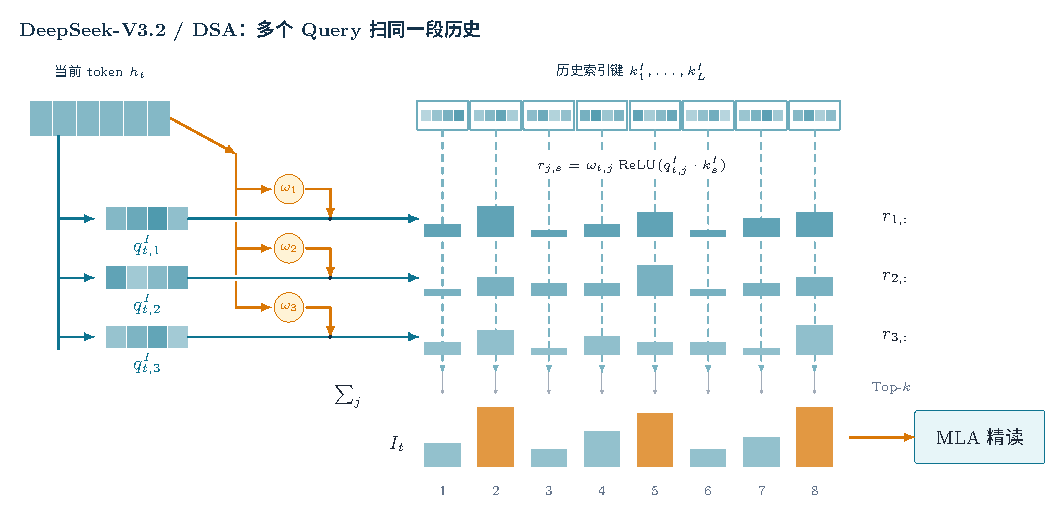
\includegraphics[width=\textwidth]{dsa_indexer.pdf}
\caption{上方每张小卡片是一个历史 token 的索引键。当前 token 生成多个 query 和对应的标量权重；每个 head 扫过同一段历史，形成一条非负的加权贡献。按历史位置逐列求和得到一条分数向量，橙色峰值是 Top-\(k\)，随后由 MLA 精读。}
\label{fig:deepseek-dsa}
\end{figure}

图 \ref{fig:deepseek-dsa} 中，当前 query 可以选到相距很远的历史位置。V2 的 MLA 缩小每张历史卡片，V3.2 的 DSA 则让主注意力只精读少数卡片：一次轻量扫描加少量精细计算，降低长上下文的注意力开销。

索引器的训练分两段。先保留稠密注意力并冻结主模型，把主注意力在历史各位置上的权重汇总成目标分布 \(p_{t,:}\)，让索引器的打分分布通过 \(\mathrm{KL}\bigl(p_{t,:}\Vert\operatorname{softmax}(I_{t,:})\bigr)\) 向它靠近；这一步教索引器识别主模型实际会关注的位置。随后启用 Top-\(k\) 稀疏选择，主模型继续用语言模型损失学习，索引器继续在选中位置上对齐主注意力的分布。两路训练信号分开：主模型沿预测损失更新，索引器沿分布对齐损失更新~\cite{deepseekv32}。


\Needspace{13\baselineskip}
\section{DeepSeek-R1：用可验证奖励选择推理轨迹}

这一节动的是第 4 条轴（训练信号）。语言模型的下一 token 损失学习怎样续写训练文本；数学答案和代码测试还提供了对整条回答的可验证反馈。DeepSeek-R1 在可验证任务的后训练中，把这类奖励与 GRPO 结合~\cite{deepseekr1}：同一道题由当前模型采样多条推理轨迹，判题器检查最终答案或代码结果，再比较同组轨迹的得分。若第 \(i\) 条轨迹得到奖励 \(r_i\)，核心比较量是式 \eqref{eq:grpo-advantage} 的组内标准化优势 \(A_i\)，它表示这条轨迹比同题其他尝试好多少。GRPO 按式 \eqref{eq:grpo-loss} 用它提高组内较好轨迹的生成概率，降低较差轨迹的生成概率，并约束策略不要一次改变过大。图像化地看，训练在同题的多条候选路径中反复强化成功路径；推理时，模型依据更新后的参数逐 token 生成推理过程和答案，判题器与组内比较只出现在训练环节。


\section{Kimi Linear：固定工作记忆加可翻查的历史}

这一节动的是第 1 条轴（历史读取）。完整注意力像一本可逐页翻查的档案：每个历史 token 都留下记录，长上下文的缓存和读取量随之增长。固定大小的递推状态像工作记忆，更新成本稳定，却会把许多过去的关联挤进同一份状态。Kimi Linear 沿层的深度方向重复“KDA、KDA、KDA、MLA”这一组：同一 token 依次经过三层 KDA，再经过一层 MLA。KDA 层维护固定大小的状态，MLA 层则保留可按内容寻找较早 token 的压缩历史~\cite{kimilinear}。

KDA 的关键是怎样维护这份有限状态。新 token 到来时，先按通道衰减过时关联，再用当前 key 从旧状态读出一个预测值，只把预测误差写回，最后由 query 读取更新后的状态。图 \ref{fig:kda-computation} 中的\textbf{衰减—纠错—读取}就是一次更新的全部动作：衰减控制保留多久，纠错减少新旧关联相互干扰。状态大小保持固定，周期性的 MLA 负责找回需要精确定位的历史细节。

\begin{figure}[H]
\centering
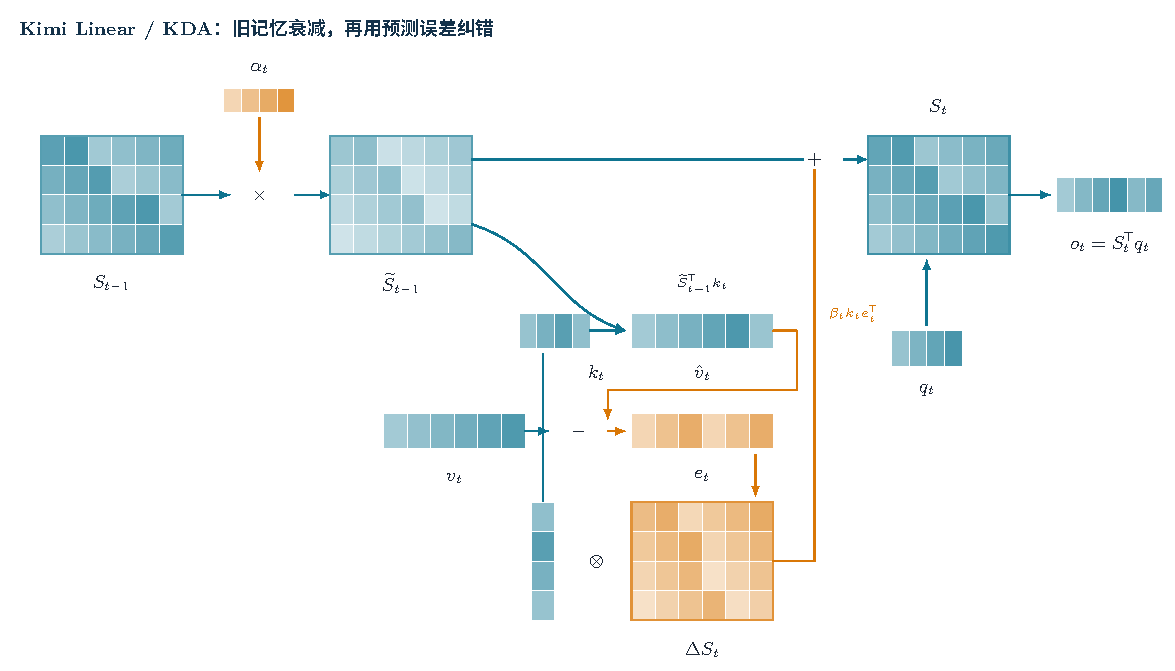
\includegraphics[width=\textwidth]{kda_computation.pdf}
\caption{KDA 把固定状态当作可修订的工作记忆：逐通道衰减旧关联，写入当前预测误差，再用 query 读取。}
\label{fig:kda-computation}
\end{figure}

图中的更新可以写成一条递推式。令 \(S_{t-1}\in\R^{d_v\times d_k}\) 为上一 token 留下的矩阵状态，方向与第 \ref{chap:transformer} 章线性注意力的 \(S_t\) 相同；\(\alpha_t\) 是每个 key 通道各自的保留比例，\(\beta_t\) 控制本次写入强度，\(q_t,k_t,v_t\) 来自当前输入：
\begin{equation}
\begin{aligned}
\widetilde S_{t-1}&=S_{t-1}\operatorname{Diag}(\alpha_t),\\
S_t&=\widetilde S_{t-1}+\beta_t\bigl(v_t-\widetilde S_{t-1}k_t\bigr)k_t^{\mathsf T},\qquad o_t=S_tq_t.
\end{aligned}
\label{eq:kda-update}
\end{equation}
第一行逐通道保留旧记忆；第二行先用当前 key 从旧状态读出预测 \(\widetilde S_{t-1}k_t\)，再把它与当前 token 的 value \(v_t\) 的差写回，最后用 query 读出 \(o_t\)。这正是图 \ref{fig:kda-computation} 的\textbf{衰减—纠错—读取}，也说明 KDA 如何用固定大小的状态持续修订键值关联~\cite{kimilinear}。

训练时，\(q_t,k_t,v_t,\alpha_t,\beta_t\) 都由可学习的投影和门控从输入产生；下一 token 损失通过 KDA 的状态更新及 MLA 层一起反传。长序列可分块并行计算块内结果，块与块之间传递状态。推理时每生成一个 token，KDA 层更新一次 \(S_t\)，MLA 层则把该 token 的短内容摘要和位置键加入缓存。前者的状态大小固定，后者承担按位置找回远处细节的任务~\cite{kimilinear}。


\section{DeepSeek-V4：多条残差流与分层历史摘要}

这一节动的是第 3 条轴（层间信息）和第 1 条轴（历史读取），末尾再涉及第 4 条轴（训练信号）。长模型同时沿两个方向积累信息：深度方向经过许多层，序列方向经过许多 token。DeepSeek-V4 分别改写这两条路径：流形约束超连接（Manifold-Constrained Hyper-Connections，mHC）让层间信息在多条残差流之间稳定混合；压缩稀疏注意力（Compressed Sparse Attention，CSA）与高度压缩注意力（Heavily Compressed Attention，HCA）让长历史以不同粒度被压缩和读取~\cite{deepseekv4}。下面分别看层间混合与历史读取。

\subsection{mHC：让深层有多条稳定的信息通道}

普通残差连接让每层在同一条表示流上继续累加。mHC 把层间状态展开成多条并行流：每层先从这些流中读出输入，算出注意力或 FFN 的新信息，再把新结果写回多条流~\cite{deepseekv4,mhc}。图 \ref{fig:mhc} 的上路负责本层读写，下路负责旧信息在各流间继续传递。

反复混合多条流容易放大或压低某些方向。mHC 约束流间混合权重为非负，且每行、每列的权重和接近 1；这样旧信息在各流间重新分配时保持受控的尺度。改动的亮点是增加层间信息通道，同时约束连续混合的稳定性；注意力和 FFN 仍处理通常宽度的输入。

把第 \(l\) 层的多条残差流记为 \(X_l\)，本层计算记为 \(\mathcal F_l\)，一次更新可写成
\begin{equation}
X_{l+1}=B_lX_l+C_l\mathcal F_l(A_lX_l),\qquad
B_l\mathbf 1=\mathbf 1,\quad \mathbf 1^{\mathsf T}B_l=\mathbf 1^{\mathsf T},\quad B_l\geq 0.
\label{eq:mhc-streams}
\end{equation}
\(A_l\) 从多条流读出本层输入，\(C_l\) 把新结果写回多条流，\(B_l\) 负责旧信息在流之间传递。训练时先从输入生成这些混合权重，再通过行、列归一化把 \(B_l\) 约束到式中的范围；预测损失通过整个读写过程反传。推理时，同一更新逐层作用于每个 token 的表示，无须改变注意力和 FFN 的内部宽度~\cite{deepseekv4,mhc}。

\begin{figure}[ht]
\centering
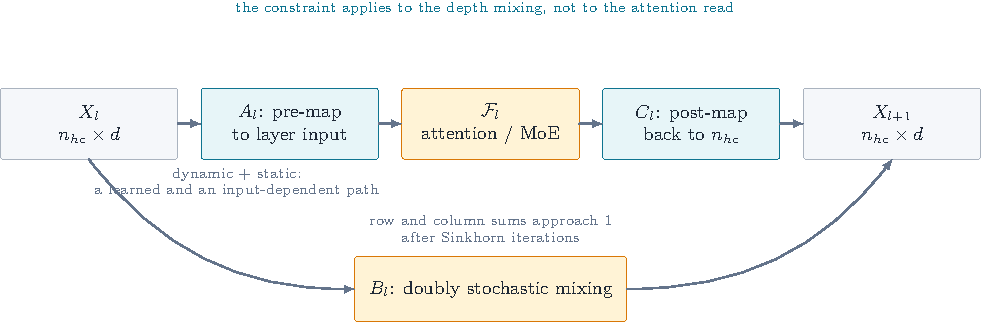
\includegraphics[width=\textwidth]{mhc.pdf}
\caption{从单条残差流到多条并行流：mHC 从多流读入子层，把新输出写回多流，并约束旧流之间的混合。}
\label{fig:mhc}
\end{figure}

\subsection{CSA/HCA：给长历史建目录和摘要}

把全部历史 token 逐一交给全局注意力，长上下文的匹配和缓存代价会不断增加。CSA 把短窗口压成较细的历史条目，再用 Lightning Indexer 找出与当前 query 最相关的少数条目；HCA 把更长的窗口压成更少的粗条目，可直接读取这些全局摘要~\cite{deepseekv4}。滑动窗口注意力（Sliding Window Attention，SWA）保留最近 token 的原始细节。这里的索引器选择压缩后的条目；V3.2 的 DSA 则选择每个历史 token 对应的 MLA 条目。

两条压缩路径共享一个基本动作：在窗口 \(W_i\) 内为各位置产生可学习的逐通道权重，再汇成一个缓存条目 \(\bar c_i=\sum_{s\in W_i}a_{i,s}\odot c_s\)，其中每个通道上的权重和为 1。CSA 的细条目吸收相邻窗口的信息，并在条目之间做 Top-\(k\) 选择；HCA 把更大的窗口压成粗条目，直接对全部粗条目做注意力。压缩权重随语言模型目标一起训练，CSA 的索引器先参考稠密注意力学习相关位置，再随稀疏注意力训练。推理时，新 token 逐步写入压缩历史；query 同时读取选中的细条目、全局粗条目和近期原始 token~\cite{deepseekv4}。

图 \ref{fig:csa-hca} 可以按\textbf{目录、摘要、近期原文}来读：CSA 先按目录挑选相关旧片段，HCA 给出较粗的全局概览，SWA 的局部窗口负责眼前细节。三种粒度一起降低长历史的直接搜索量，同时保留远处相关内容和近处精确信息。

\begin{figure}[ht]
\centering
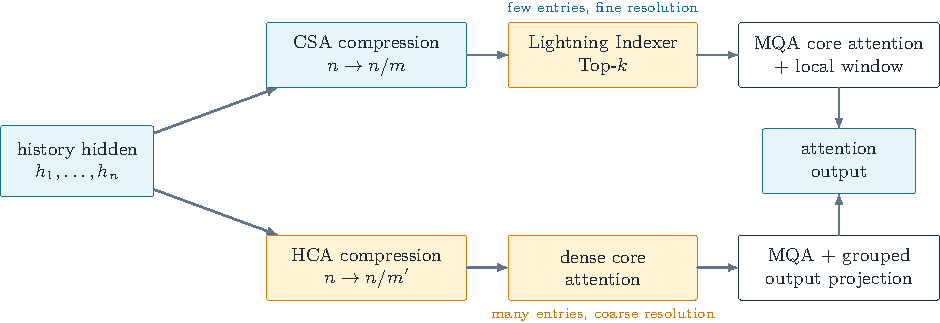
\includegraphics[width=\textwidth]{csa_hca.pdf}
\caption{CSA 在较细的压缩条目上做内容选择；HCA 读取更粗的全局摘要；局部窗口保留最近细节。}
\label{fig:csa-hca}
\end{figure}

\subsection{多领域后训练与在线蒸馏}

DeepSeek-V4 先在不同任务上分别后训练领域专长模型，再用第 \ref{sec:distillation} 节的多教师 on-policy 蒸馏把它们合进一个统一模型~\cite{deepseekv4}：统一模型在各领域的提示上自己生成回答，由该领域的专长模型在这些回答的前缀上给出下一 token 分布，按式 \eqref{eq:multi-teacher-opd} 更新，参数更新后重新采样。推理时只部署统一模型。

\section{Kimi K3：沿序列、深度和专家三处继续改进}

这一节沿第 1、3、2 条轴依次改动。Kimi K3 延续 Kimi Linear 的固定状态与可寻址历史组合，再处理三个新的限制：长序列递推的数值稳定、深层对早期表示的访问，以及大量专家之间的通信~\cite{kimik3}。图 \ref{fig:kimi-k3-block} 的上排是序列路径，下排是深度路径；专家模块放在每层 FFN 的位置。下文的注意力残差（Attention Residuals，AttnRes）处理跨层读取，稳定潜空间专家混合（Stable Latent Mixture of Experts，Stable LatentMoE）处理专家计算。

\begin{figure}[H]
\centering
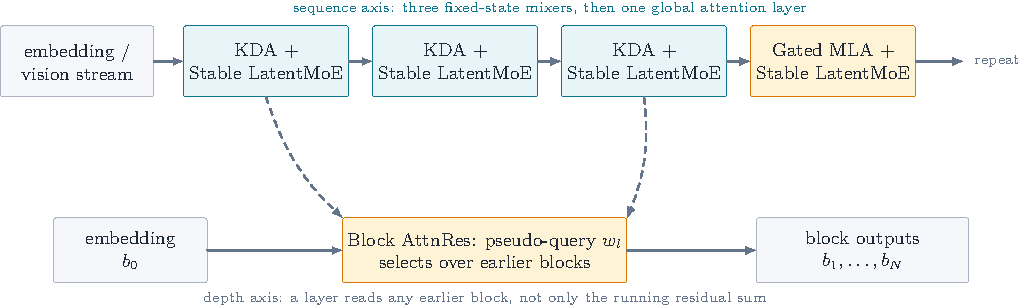
\includegraphics[width=\textwidth]{kimi_k3_block.pdf}
\caption{K3 在三处动手：KDA/Gated MLA 管序列历史，AttnRes 管跨层读取，Stable LatentMoE 管专家计算。}
\label{fig:kimi-k3-block}
\end{figure}

\subsection{序列：稳定的 KDA 与可控的全局读取}

KDA 的递推要在很长的序列上重复衰减与写入。K3 给衰减设定下界，避免反复更新时数值尺度走向极端；这提高长序列训练的稳定性。周期性的全局层继续使用 MLA，让模型直接找回较早的相关位置~\cite{kimik3}。全局注意力读出历史后，Gated MLA 再根据当前 token 对各输出通道加门控：相关通道多写入当前表示，干扰较大的通道少写入。图 \ref{fig:kimi-k3-block} 上排的三个 KDA 层与一个 Gated MLA 层体现了固定状态和全局读取的分工。

令 \(z_{t,j}\) 为 KDA 第 \(j\) 个 key 通道经过可学习缩放的衰减分数，K3 用 \(g_{t,j}=g_{\min}\operatorname{sigmoid}(z_{t,j})\)、\(\alpha_{t,j}=e^{g_{t,j}}\) 生成式 \eqref{eq:kda-update} 中的保留比例，其中 \(g_{\min}<0\)。这样 \(\alpha_{t,j}\) 有正的下界，分块并行训练时连续衰减的数值范围受到控制。对 MLA 读出的 \(\widetilde o_t\)，门控输出可写为 \(y_t=W_o[\operatorname{sigmoid}(W_gx_t)\odot\widetilde o_t]\)：当前 token 决定哪些历史通道进入下一层。训练时这些门控随下一 token 损失学习；推理时 KDA 继续逐 token 更新固定状态，MLA 缓存仍保留可按位置读取的历史~\cite{kimik3}。

\subsection{深度：AttnRes 按需翻回早期层}

普通残差让信息逐层累加；AttnRes 则保留较早层块为同一 token 产生的输出，并用它们组成当前层的输入~\cite{kimik3,attnres}。当前层 \(l\) 有一个训练得到的查询向量 \(w_l\)：它分别与各块输出的归一化表示做内积，得到每个块的匹配分数，再对所有可访问块的分数做 softmax。分数越高，该块输出在当前层输入中占的权重越大。这意味着，同一当前层面对不同 token 时，叠加先前各层输出所用的权重也可能不同；本层计算产生的新输出又成为更深层可读取的候选。图 \ref{fig:k3-attnres-depth} 将这条从已有输出到当前输入、再到新输出的路径画出来。这些块权重可以用来查看当前层主要读取了哪些较早的层。

\begin{figure}[ht]
\centering
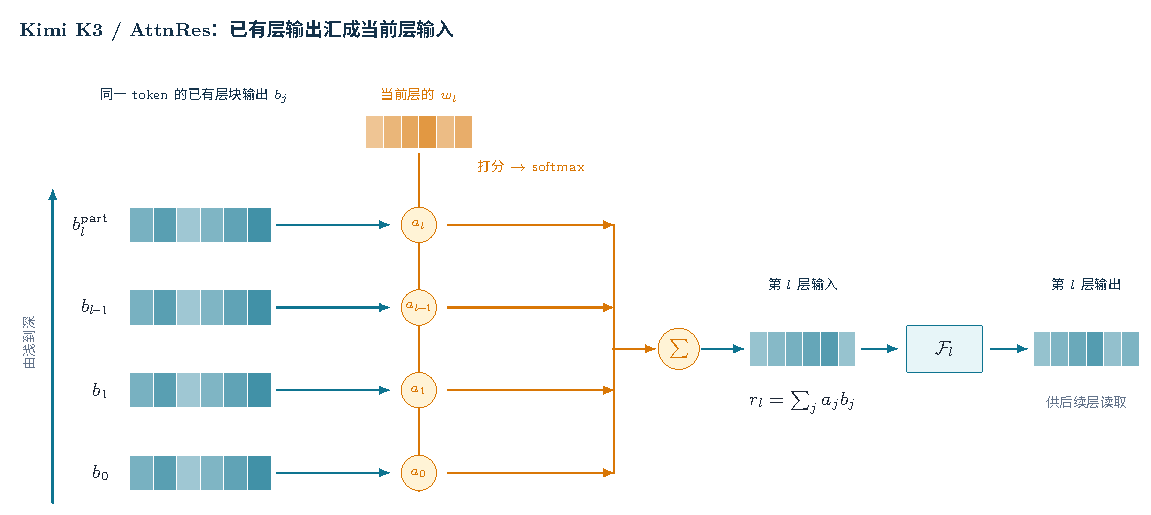
\includegraphics[width=\textwidth]{attnres_depth.pdf}
\caption{已有层块输出按当前层算出的权重汇合成输入 \(r_l\)，本层计算再产生新输出；图中的 \(a_j\) 是 \(a_{l,j}\) 的简写。}
\label{fig:k3-attnres-depth}
\end{figure}

\Needspace{9\baselineskip}
令 \(b_j\) 表示较早层块的输出或当前块已完成的部分，\(\mathcal B_l\) 是当前层可访问的块集合。打分、归一化和组成当前层输入依次写为
\begin{equation}
\begin{aligned}
s_{l,j}&=w_l^{\mathsf T}\operatorname{RMSNorm}(b_j),\\
a_{l,j}&=\frac{\exp(s_{l,j})}{\sum_{i\in\mathcal B_l}\exp(s_{l,i})},\\
r_l&=\sum_{j\in\mathcal B_l}a_{l,j}b_j.
\end{aligned}
\label{eq:attnres-block}
\end{equation}
\(\operatorname{RMSNorm}(b_j)\) 用来计算分数，控制不同层块输出的尺度差异；真正加权相加的是块输出 \(b_j\) 本身。\(r_l\) 是第 \(l\) 层的输入，经过本层计算后才产生新的输出。V4 的 mHC 同时维护多条并行残差流，K3 的 AttnRes 则从较早深度按需读取。

\subsection{专家：先压窄，再送入路由专家}

普通专家并行把模型宽度的表示发往选中的专家，跨设备传输随激活专家数增加。Stable LatentMoE 先把路由分支压到较窄的潜空间，让专家在这个空间计算，再把聚合结果映射回模型宽度；共享专家仍接收完整表示~\cite{kimik3}。若输入 \(x\in\mathbb R^d\)、压缩表示 \(z\in\mathbb R^\ell\) 且 \(\ell<d\)，\(E_i\) 是路由专家、\(p_i\) 是选中专家的混合权重，两条路径合起来可写为
\begin{equation}
z=W^{\downarrow}x,\qquad
u=\sum_{i\in\mathcal T(x)}p_iE_i(z),\qquad
y=\sum_j E_j^{\mathrm{shared}}(x)+W^{\uparrow}\operatorname{RMSNorm}(u).
\label{eq:k3-latent-moe}
\end{equation}
\begin{figure}[ht]
\centering
\begin{tikzpicture}[x=1cm,y=1cm]
  \node[softblock,minimum width=18mm,minimum height=9mm] (x) at (0.9,0) {输入 \(x\in\mathbb R^d\)};
  \node[tealblock,minimum width=25mm,minimum height=10mm] (down) at (3.4,1.25) {降维 \(W^{\downarrow}\)\\\(z\in\mathbb R^\ell\)};
  \node[orangeblock,minimum width=29mm,minimum height=10mm] (route) at (6.9,1.25) {Top-\(k\) 路由\\专家处理 \(z\)};
  \node[tealblock,minimum width=25mm,minimum height=10mm] (mix) at (10.25,1.25) {加权聚合\\RMSNorm};
  \node[tealblock,minimum width=22mm,minimum height=10mm] (up) at (13.1,1.25) {升维 \(W^{\uparrow}\)\\回到 \(d\) 维};
  \node[orangeblock,minimum width=33mm,minimum height=10mm] (shared) at (6.9,-1.15) {共享专家处理完整 \(x\)};
  \node[softblock,minimum width=17mm,minimum height=9mm] (out) at (13.1,-1.15) {相加得 \(y\)};
  \draw[flow] (x.north east) -- (down.west);
  \draw[flow] (down.east) -- (route.west);
  \draw[flow] (route.east) -- (mix.west);
  \draw[flow] (mix.east) -- (up.west);
  \draw[flow] (x.south east) -- (shared.west);
  \draw[flow] (shared.east) -- (out.west);
  \draw[flow] (up.south) -- (out.north);
\end{tikzpicture}
\caption{Stable LatentMoE 的两条路径：路由专家接收低维表示 \(z\)，共享专家接收完整表示 \(x\)，两路输出回到同一宽度后相加。}
\label{fig:k3-latent-moe}
\end{figure}

图 \ref{fig:k3-latent-moe} 中，路由专家收到较窄的任务摘要 \(z\)，跨设备传送的也是这份低维表示。聚合后的归一化控制路由分支的尺度；专家内部的 SiTU-GLU 用平滑的 \(\beta\tanh(a/\beta)\) 限制大激活。训练时，下一 token 损失更新降维与升维投影、路由器、共享专家和选中的路由专家；Quantile Balancing 则根据一批 token 的路由分数分位数直接调整下一步的专家选择偏置，使各专家接近目标负载。推理时依据路由分数与训练结束时保留的偏置选专家，只向路由专家传送低维 \(z\)，再把两条路径的结果相加~\cite{kimik3}。

\chapter{统计学习与数据模式：常见陷阱}
\label{chap:data-patterns}

\begin{keybox}[训练目标只看见经验分布]
模型最终学到什么由数据分布、目标函数和采样过程共同决定。这里把前文所有模型重新放回同一个审计闭环：训练集是否代表部署分布，loss 是否奖励真正关心的性质，生成器是否覆盖模式与尾部，服务中的筛选和合成数据回流是否悄悄改变下一轮经验分布。
\end{keybox}

\section{数据分布比数据总量更重要}

若训练集由多个来源混合而成，经验分布其实是 \(\hat\pi=\sum_k\alpha_k\hat\pi_k\)。改变比例 \(\alpha_k\) 就改变了被优化的目标，即使总 token 数不变。科学数据还经常存在温度、压力、相区、几何尺寸或实验设备的分层结构；逐样本随机切分时，同一次实验或模拟的相邻记录可能同时进入训练和测试，使测试结果偏乐观。若反复把模型生成的数据用于后续模型的训练，而缺少真实数据校正，稀有模式还可能逐轮减少~\cite{shumailov2024curse}。

\begin{table}[ht]
\centering\small
\begin{tabularx}{\textwidth}{>{\bfseries}p{29mm} X X}
\toprule
数据模式 & 可能后果 & 验证项目\\
\midrule
长尾 & 高频 token 主导平均 loss；占 2\% 的稀有模式在平均 NLL 中也只占 2\% 权重 & 按频率、领域、长度、语言和任务分层报告\\
重复/污染 & 验证 loss 与 benchmark 被高估，记忆被误判为推理；相邻帧的相似度可以接近 1 & 近似去重、时间切分、训练-测试相似度审计\\
混合分布 & 模型学到来源比例和格式偏差 & 保存来源标签，报告每个子分布指标\\
轨迹相关 & 同一实验或模拟的相邻状态高度相似；逐样本随机切分会让测试结果偏乐观 & 让同一对象或整条轨迹只进入一个数据集；预测未来时按时间切分\\
非平稳 & 数据分布随时间变化，未来数据与训练数据不同，旧测试结果可能失效 & 按时间留出较新数据，记录条件变化，持续监测模型表现\\
合成递归 & 反复用上一代模型生成的数据训练下一代，稀有模式可能逐轮减少，错误可能累积 & 保留真实数据，记录生成器、筛选规则与合成比例，并检查稀有模式\\
\bottomrule
\end{tabularx}
\caption{数据审计应围绕分布结构展开，样本数量只是其中一项。}
\label{tab:data-patterns}
\end{table}

“轨迹相关”例如：同一分子动力学轨迹的相邻帧很相似。若分别放入训练集和测试集，模型可能靠识别近似重复的状态得分，未必能预测新轨迹。评估新轨迹时，应将整条轨迹只放入训练、验证、测试中的一组；评估未来状态时，按时间切分，并避免相似帧跨组。

“非平稳”指数据的统计分布随时间改变。例如，用某实验装置上半年的测量训练模型，后来更换传感器或调整工作温度，下半年的读数范围和噪声水平可能变化。即使模型在随机抽出的历史测试集上表现很好，也未必适用于新条件。应留出较晚时间段的数据单独测试，按设备和实验条件分层报告，并在部署后检查输入分布及模型误差是否变化。

“合成递归”是指模型 A 生成样本训练模型 B，模型 B 再生成样本训练模型 C，如此反复。如果每轮生成或筛选都漏掉少见的样本，下一轮的训练数据就更缺少这些样本，模型可能越来越不擅长生成它们。若每一轮丢掉 10\% 的稀有模式，十轮后只剩约 \(0.9^{10}\approx0.35\)。风险大小取决于合成数据的质量和占比、筛选方式，以及每轮是否继续加入足够的真实数据。

\section{训练与采样的错位}

teacher forcing 在第 \(t\) 步使用真实的 \(x_{<t}\)，但部署时模型接收到的是自己采样的前缀。一个小的局部错误会改变后续条件分布，形成 exposure bias。缓解办法包括 scheduled sampling~\cite{bengio2015scheduled}、数据增强、从模型生成的轨迹上训练、搜索/验证、过程监督和更强的后训练；这些方法都会改变统计目标，比较时应在同一目标下进行。

\section{似然、样本质量与模式覆盖}

判别式分类有真实类别标签，受试者工作特征曲线下面积（area under the receiver operating characteristic curve，ROC-AUC）等指标可以概括模型区分正负样本的能力。ROC-AUC 汇总了不同判别阈值下的表现。生成模型通常没有一个被广泛接受、又能同时概括主要性能维度的单一指标，因此评价往往比分类更复杂。即使在图像生成中，弗雷歇 Inception 距离（Fréchet Inception Distance，FID）等自动指标也难以充分判断视觉自然度、局部瑕疵或内容是否符合条件；许多实际比较仍需要人眼评审。

评价生成模型要分别回答：模型给真实测试样本多大概率；从模型抽出的单个样本是否可信或有用；大量生成样本能否覆盖真实分布的不同模式及长尾。似然或负对数似然（NLL）回答第一个问题。较高的测试似然说明模型对已观测数据分配了较多概率质量；单张样本是否自然、采样温度与引导是否合适，需要另外的指标。高维图像模型中，平均对数似然与视觉保真度可以相当独立~\cite{theis2016evaluation}。

反过来，生成样本看起来很好，也可能只来自真实分布的一小部分。设真实数据有几种不同的构象或图像类别，一个生成器只产生其中最容易的一类，每个样本都很逼真，但其他模式的概率几乎为零；这就是\textbf{mode collapse（模式坍缩）}。采样时只保留高分结果也可能提高单样本质量，同时丢掉多样性。因而至少要分别报告\textbf{保真度}与\textbf{覆盖度}，并针对稀有模式或物理相区单独检查，不能让一个平均分数代替所有结论。

\Needspace{10\baselineskip}
\section{常见生成指标各自在测什么}

为了避免把“拟合真实数据”“单张样本可信”和“覆盖全部模式”混成一个分数，下面分别说明常用指标的比较对象。

下表中的困惑度（perplexity，PPL）用于评价语言模型。这里的 Inception 特征是指：将图像输入在 ImageNet 上预训练的 Inception-v3 分类网络，取分类层之前的中间激活向量（通常取最后的全局平均池化层输出），作为这张图像的数值表示。FID 先把真实图像和生成图像分别变成这样的特征向量，再比较两组向量的均值和协方差；因此它衡量的是选定特征空间中的整体统计差异。

\begin{table}[ht]
\centering\small
\begin{tabularx}{\textwidth}{>{\bfseries}p{34mm} X X}
\toprule
指标 & 实际比较的对象 & 主要局限\\
\midrule
测试集 NLL / PPL & NLL 是真实测试样本的平均负对数概率；PPL 是平均 token NLL 的指数 & 衡量给真实数据的概率，不直接衡量抽样文本是否有用；不同数据集或 tokenizer 的 per-token 数值不宜直接比较\\
FID & 比较真实图像与生成图像在 Inception 特征中的均值和协方差，越低表示这两个统计摘要越接近 & 把保真度与覆盖度混在一个数里；依赖特征网络、预处理和样本数，不能保证局部模式都被覆盖\\
Precision/Recall & 在特征空间中，Precision 估计生成样本靠近真实区域的比例；Recall 估计真实区域被生成样本覆盖的程度 & 能分开观察样本质量与覆盖度，但依赖特征表示、邻域定义及样本量\\
\bottomrule
\end{tabularx}
\caption{三个常用指标分别观察概率拟合、图像特征统计，以及生成样本的保真度和覆盖度。FID 与生成模型 Precision/Recall 的定义见相应原始工作~\cite{heusel2017fid,kynkaanniemi2019precisionrecall}。}
\label{tab:generation-metrics}
\end{table}

对自回归语言模型，若测试集共有 \(N\) 个被计分 token，\(\mathrm{PPL}=\exp\!\bigl[-N^{-1}\sum_t\log p_\theta(x_t\mid x_{<t})\bigr]\)。所以 PPL 只是把平均 token NLL 换一个尺度；长回答是否重复、事实是否正确、条件是否满足，需要另外检查。FID 与生成模型的 Precision/Recall 主要用于图像；在分子或物理构型上，应改用与对象相关的结构描述和观测量。

\section{校准与分布外泛化}

对条件生成还要检查生成结果是否满足给定条件；对科学数据还要检查守恒律、对称性和有效结构。校准问题可以问：模型给出 0.8 的事件概率时，长期频率是否接近 0.8？OOD（Out-of-Distribution，分布外）问题可以问：模型在远离训练支撑集时是否仍给出过高置信度？这两个问题都不能由单一平均 NLL、FID 或样本外观解决。

\Needspace{9\baselineskip}
\section{变分训练的诊断}

\begin{itemize}
  \item VAE：记录 reconstruction、KL、每维 KL、潜变量互信息和 posterior samples。
  \item Flow：检查 log-det 的数值范围、逆变换误差、尾部样本和 Jacobian 条件数。
  \item Diffusion：按噪声时间或信噪比分层报告 denoising loss，检查采样步数、solver、guidance 和 OOD。
  \item EBM：检查 MCMC 的自相关、有效样本数、不同初始化的混合、能量与物理量之间的关系。
  \item 自回归：检查长度分层 loss、token 频率、校准、重复率、temperature/top-$p$ 敏感性和长程一致性。
\end{itemize}

\section{物理与科学数据的额外约束}

如果数据具有群对称性，应使用 invariant/equivariant 架构或在数据/损失中明确处理；如果生成对象必须满足约束，应使用参数化保证、投影、惩罚、条件变量或后验筛选。对 Boltzmann 任务，须分别报告结构有效率、能量分布、温度、自由能差、相关函数和模式覆盖；“样本看起来像”只是最低层证据。

\begin{figure}[ht]
\centering
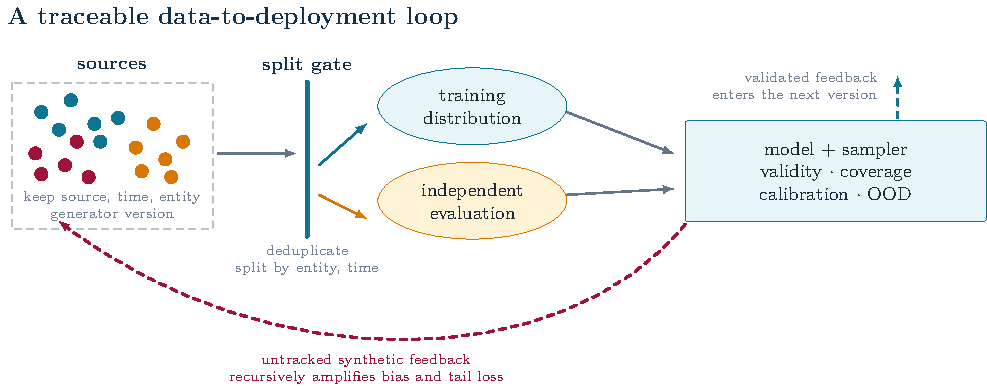
\includegraphics[width=\textwidth]{data_audit_loop.pdf}
\caption{审计闭环必须保留“样本来自哪里、如何切分、在哪个分布上评价、哪些生成样本被回流”四类信息。只有通过独立分布评估和物理约束的输出才能有条件进入下一版数据；无标记回流会把偏差和尾部丢失递归放大。}
\label{fig:audit-loop}
\end{figure}

\chapter{把生成模型放回科学计算}
\label{chap:science}

\begin{keybox}[把分布问题换回物理问题]
前面各章的模型都可以放回科学计算：能量给出目标分布，样本给出构型，密度给出自由能。这一章看几个已经走通的接口——有限温采样、重整化群、分子与晶体结构、量子线路与量子态——并在每个接口上说清楚：模型生成的对象是什么，评价它的物理量又是什么。
\end{keybox}

\section{统计物理：从能量到平衡样本}

以 Ising 自旋为例，一个构型 \(\sigma=(\sigma_1,\ldots,\sigma_N)\) 的能量由相互作用和外场给定，有限温的目标分布是 \(p_\beta(\sigma)=e^{-\beta H(\sigma)}/Z_\beta\)，其中 \(\beta=1/(k_{\mathrm B}T)\)。难点是构型数随系统大小指数增长，配分函数 \(Z_\beta\) 和观测量的平衡平均通常无法直接求和。生成模型可以构造容易采样的试探分布，再用已知能量引导它接近目标分布。

对连续的多体坐标，Boltzmann generator 用可逆流把易采样的基分布映射到目标构型空间~\cite{kim2019boltzmann}。模型给出候选样本及其密度后，可以按目标玻尔兹曼权重重新加权，或用 MCMC 修正偏差。模型的直接作用是快速产生物理上合理的候选构型；加权后的样本是否代表目标温度下的平衡测度，是另一个问题。

若用变分自由能训练 Boltzmann generator，抽样从参数无关的基分布开始，连续构型由可逆流映射得到；能量和模型对数密度的梯度沿这一映射回传，使用第 \ref{sec:gradient-estimator-map} 节的重参数化路径。

生成模型还可以当重要性采样的 proposal。设从 \(q_\theta\) 采样 \(x\)，目标权重是 \(w(x)=e^{-\beta E(x)}/q_\theta(x)\)；加权平均给出目标测度下的观测量，配分函数由权重的均值估计。若 \(q_\theta\) 只在部分区域有概率，权重的方差会很大；退火重要性采样把一列中间温度串起来，让相邻分布的重叠更大，得到更稳的自由能差估计。这里生成模型提供覆盖多个模式的 proposal，最终的自由能仍由权重和物理能量决定。

\section{有限温变分计算：自回归网络}

传统变分平均场常把试探分布写成独立单点概率的乘积，因而难以描述自旋之间的关联。变分自回归网络（Variational Autoregressive Network，VAN）保留链式分解 \(q_\theta(\sigma)=\prod_i q_\theta(\sigma_i\mid\sigma_{<i})\)，但让后面的条件概率读取前面已生成的自旋~\cite{wu2019variational}。每个条件概率都归一化，所以完整构型的 \(q_\theta(\sigma)\) 可计算；逐个抽取自旋便得到独立生成的完整构型，无需等待马尔可夫链混合。

已知 \(H\) 时，可以直接最小化变分自由能 \(F_\theta=\mathbb E_{q_\theta}[H(\sigma)+\beta^{-1}\log q_\theta(\sigma)]\)。它满足 \(F_\theta-F_\beta=\beta^{-1}\KL(q_\theta\Vert p_\beta)\geq 0\)，因此给出真实自由能的上界，也把降低能量与保留熵放在同一目标中。训练后，用 \(\sigma\sim q_\theta\) 的样本估计能量、磁化和关联函数；若要准确估计目标玻尔兹曼平均，还需考虑分布误差并使用适当的重加权或采样修正。VAN 是比独立变量平均场更灵活的变分分布，优化目标仍是有限温的自由能。

VAN 从依赖 \(\theta\) 的离散分布 \(q_\theta(\sigma)\) 抽取自旋，无法沿自旋取值反向传播；训练自由能时使用第 \ref{sec:gradient-estimator-map} 节的 score-function 路径，以构型的局部自由能 \(H(\sigma)+\beta^{-1}\log q_\theta(\sigma)\) 加权 \(\nabla_\theta\log q_\theta(\sigma)\)，并可减去 baseline 降低方差。

\section{流模型与重整化群}

重整化群试图逐层分离短尺度涨落，留下描述长尺度行为的有效变量。Li 与 Wang 的神经网络重整化群用分层可逆变换连接物理构型和多尺度潜变量~\cite{li2018neuralrg}：每一层提取部分自由度，并让潜变量之间的统计依赖逐渐减弱；反向变换则从简单的独立潜变量生成物理构型。这使“粗粒化后保留什么信息”成为可以通过模型学习的问题。

可逆性还允许通过 Jacobian 计算生成构型的概率密度，并用变分自由能训练该映射。训练后的潜变量按层对应不同尺度的涨落，可以检查它们的相关性，观察模型是否实现了预期的尺度分离。流模型在这里承担可计算密度与生成样本的工具；分层结构和尺度分离的检验，才赋予这一具体模型重整化群的解释。

对这类连续可逆流，变分自由能中的模型样本由固定基分布经可微映射生成，训练仍沿第 \ref{sec:gradient-estimator-map} 节的重参数化路径求导。

\section{分子构象与材料结构}

若已知分子的原子种类和连接关系，生成对象可以是所有原子的三维坐标；扩散模型或 Flow Matching 从简单噪声逐步得到候选构象。模型应尊重平移、旋转及同种原子置换带来的等价性，同时避免不合理的键长、碰撞和错误手性。等变架构把群作用写进网络结构，例如对坐标做等变的消息传递，或在损失中加入不变量；约束可以用参数化保证、投影、惩罚或后验筛选实现。评估不能只看坐标是否像训练样本，还要检查能量、构象多样性及目标性质，并说明这些量是在生成后直接计算还是经过物理松弛得到。

晶体生成还需要处理元素组成、周期性晶胞和晶胞内原子位置。若给定目标性质作为条件，得到的结构仍须满足组成、对称性和稳定性约束，再由独立的物理计算验证性质。这个例子说明，条件生成给出的是候选分布，后续筛选与验证决定候选能否成为可信的科学结果。

\section{可微量子线路结构搜索}

设计变分量子线路时，既要选择每一位置放什么门，也要调节门的连续参数。门的种类和连接方式是离散变量，直接枚举所有线路会迅速遇到组合爆炸。可微量子架构搜索（Differentiable Quantum Architecture Search，DQAS）先限定门集合、线路位置和可用连接，再用可训练的概率分布 \(p_\alpha(A)\) 抽样线路结构 \(A\)~\cite{zhang2022dqas}。对抽到的线路计算任务损失 \(L(A,\theta)\)，例如制备态的能量或逼近目标酉矩阵的误差；优化 \(\mathbb E_{A\sim p_\alpha}[L(A,\theta)]\) 中的结构分布参数 \(\alpha\) 与门参数 \(\theta\)，最后选出具体线路并检验其性能。

DQAS 的“可微”是指期望损失对概率分布参数可以求梯度；一次离散的门选择本身没有连续导数。概率模型让搜索在门组合之间分配计算预算，并把线路搭建与参数优化联系起来。得到的线路仍需在实际任务上重新评估，因为搜索空间限制和抽样梯度的噪声都会影响结果。

优化线路结构分布 \(p_\alpha(A)\) 时，抽到的门结构 \(A\) 是离散的，因此其参数 \(\alpha\) 使用第 \ref{sec:gradient-estimator-map} 节的 score-function 路径，以 \(L(A,\theta)\nabla_\alpha\log p_\alpha(A)\) 估计梯度；给定线路后的连续门参数 \(\theta\) 则通过相应的量子线路梯度方法更新。

\section{神经网络量子态：基态与动力学}

前一节的模型生成线路结构；如果目标是多体系统的量子态本身，可以用神经网络表示波函数振幅 \(\psi_\theta(s)=\langle s\mid\psi_\theta\rangle\)，其中 \(s\) 是选定基底中的构型~\cite{carleo2017nqs}。求基态时，按 \(|\psi_\theta(s)|^2\) 采样构型，用哈密顿量计算变分能量 \(E_\theta=\langle\psi_\theta|H|\psi_\theta\rangle/\langle\psi_\theta|\psi_\theta\rangle\)，再调节网络参数降低能量。变分原理保证 \(E_\theta\) 不低于真实基态能量；能量之外还应检查相关函数等目标观测量。

研究动力学时，从初态出发，把薛定谔方程给出的波函数变化投影到网络参数能够表示的变化方向，再按时间步更新网络参数~\cite{carleo2017nqs}。这种时间依赖变分方法用同一波函数表示跟踪实时演化，但长期精度取决于网络表达能力、采样误差和时间积分误差。这里生成模型的角色是表示带相位的量子振幅；它与只生成某个测量基下比特串概率的 Born machine 有不同的物理目标。

对按 \(|\psi_\theta(s)|^2\) 抽到的离散构型，变分蒙特卡洛也用对数导数把采样分布对参数的依赖写入能量梯度；这与第 \ref{sec:gradient-estimator-map} 节的 score-function 路径相通，权重由哈密顿量给出的局部能量决定。

\section{量子与张量网络生成模型}

前一节用波函数研究量子态本身；若只想生成选定基底下的构型，可以把振幅的模方当作概率分布。同一 Born 规则可以配两种表示：参数化量子线路在测量时直接给出样本，矩阵乘积态（Matrix Product State，MPS）则用一串可收缩的张量表示振幅。两者都可以作为离散构型的生成模型，但训练和采样所需的计算不同。

\textbf{量子线路 Born machine。}QCBM~\cite{liu2018qcbm} 把 \(U_\theta|0^n\rangle\) 测得比特串 \(s\) 的概率写为 \(p_\theta(s)=|\langle s|U_\theta|0^n\rangle|^2\)。第 \ref{sec:mmd-qcbm} 节已说明：运行线路即可采样，真实样本与测量样本可用 MMD 比较，参数移位法则用多次线路运行估计训练梯度。放到多自旋构型任务时，除分布差异外，还应检查磁化和关联函数等任务相关观测量。有限测量次数难以准确估计稀有构型的逐点概率，这是用样本差异训练时仍需注意的限制。

\textbf{张量网络 Born machine。}对 \(s=(s_1,\ldots,s_n)\)，MPS 把振幅写为一串矩阵的乘积，再由模方得到归一化概率~\cite{han2018mps}：
\begin{equation}
 \psi_\theta(s)=A^{[1]}_{s_1}A^{[2]}_{s_2}\cdots A^{[n]}_{s_n},\qquad
 p_\theta(s)=\frac{|\psi_\theta(s)|^2}{\sum_{s'}|\psi_\theta(s')|^2}.
\end{equation}
这里首尾张量的边界维度为 1，所以矩阵乘积最终是一个标量；相邻张量之间的内部维度称为键维 \(D\)。给定构型时，可直接收缩矩阵链计算其概率；生成时则逐位计算条件概率 \(p_\theta(s_i\mid s_{<i})\)、采样并继续收缩，直到得到整条构型。训练可最小化数据的负对数似然，梯度沿张量收缩回传。较大的 \(D\) 容许更多跨位置关联，也增加存储和收缩成本；固定的小键维适合主要由较短程或较低纠缠结构决定的分布。与量子线路的测量采样相比，MPS 的逐点概率和归一化可以通过经典张量收缩计算，但成本仍随键维增长。

这两类 Born machine 学到的都是所选测量基下的 \(p_\theta(s)\)。相同的概率可以对应不同相位的波函数，因此只检验该基底的样本统计，不能判断完整量子态是否正确；若目标是量子态，还需额外测量基或对相位敏感的观测量。

回到第 \ref{chap:probability-language} 章的问题：给定目标性质 \(y^\star\)，怎样在合理的结构上采样 \(p(x\mid y^\star)\)。这一章的例子给出了同一条链的不同实现方式：生成模型提供 \(p(x)\) 或 \(p(x\mid c)\)，性质预测器与物理计算提供 \(p(y\mid x)\) 的近似或验证，权重、引导、筛选和重加权把两者接起来。链条的每一环都可能引入误差，因此最终报告的应是经过独立物理检验的候选。哪一类模型适合哪个接口，取决于对象是离散还是连续、能量是否可算、以及能否承受 MCMC 或 ODE 的采样成本。


\appendix
\chapter{阅读索引}

\begin{table}[ht]
\centering\small
\begin{tabularx}{\textwidth}{>{\bfseries}p{28mm} X X}
\toprule
章节 & 主题 & 主要技术对象\\
\midrule
第一章 & 生成模型的概率语言与自由能 & 分布、条件生成、KL、自由能\\
第二章 & 主流生成模型的表达、训练与采样 & 自回归、VAE、Flow、GAN、扩散与能量模型\\
第三章 & Transformer 的输入、信息流和内部组件 & token、Q/K/V、注意力变体、归一化、FFN、MoE\\
第四章 & 多模态：理解与生成 & 视觉 token 预算、对比学习与互信息、VLM 连接器、条件注入、统一多模态模型\\
第五章 & 预训练、微调与奖励 & MLE、SFT、LoRA、偏好优化、可验证奖励\\
第六章 & 训练系统 & AdamW、Muon、QK-Norm、混合精度、训练显存账本、DP/TP/EP\\
第七章 & 推理系统 & prefill/decode、KV cache、FlashAttention、PD 分离与服务指标\\
第八章 & 智能体系统 & 主循环、工具调用、上下文缓存成本、skill 与 memory、agentic search、子智能体、pass@k 与 pass\(^k\)\\
第九章 & DeepSeek 与 Kimi 架构案例 & MLA、DSA、mHC、CSA/HCA、KDA、AttnRes、Stable LatentMoE\\
第十章 & 数据与生成结果的评价 & 模式覆盖、FID、Precision/Recall、perplexity、OOD\\
第十一章 & 生成模型在科学计算中的应用 & 有限温 VAN、神经重整化群、分子材料、线路搜索、量子态、量子线路与张量网络生成\\
\bottomrule
\end{tabularx}
\caption{各章主题与主要技术对象的阅读索引。}
\label{tab:content-map}
\end{table}

\chapter{公式速查与符号表}

\begin{longtable}{p{36mm} p{100mm}}
\toprule
符号 & 含义\\
\midrule
\endhead
\(\pi(x),\ p_\theta(x)\) & 目标或数据分布；由参数 \(\theta\) 定义的生成模型。\\
\(\E_p[f(x)]\) & 在分布 \(p\) 下对 \(f(x)\) 取期望。\\
\(\KL(p\Vert q)\) & \(\E_p[\log p(x)-\log q(x)]\)，方向不可交换。\\
\(z,\ q_\phi(z\mid x)\) & 潜变量；VAE 中由编码器给出的变分后验。\\
\(E(x),\ Z,\ \beta\) & 能量、配分函数及逆温；\(p(x)=e^{-\beta E(x)}/Z\)。\\
\(F[q]\) & 变分自由能，\(F[q]=\E_q[E]-T S[q]\)。\\
\(\bar\alpha_t,\ a_t,\ b_t\) & 扩散过程中累计保留的信号比例；\(a_t=\sqrt{\bar\alpha_t}\)、\(b_t=\sqrt{1-\bar\alpha_t}\) 为累计信号与噪声幅度。\\
\(\epsilon_\theta(x_t,t)\) & 模型预测的累计噪声。\\
\(\nabla_x\log p_t(x)\) & score，即时刻 \(t\) 对数密度对 \(x\) 的梯度。\\
\(T\) & 在序列模型中为序列长度，在扩散模型中为总步数；温度也常记为 \(T\)，由 \(\beta=1/(k_{\mathrm B}T)\) 区分。\\
\(\tau,\ \mathcal V\) & token 采样温度；词表。\\
\(Q,K,V\) & 注意力中的查询、键和值矩阵。\\
\(L,\ n_{kv},\ d_h\) & Transformer 层数、KV head 数、每个 head 的维度。\\
\(c_t^{KV}\) & MLA 为位置 \(t\) 缓存的低维内容摘要。\\
\(S_t\) & 线性注意力或 KDA 汇总历史信息的矩阵状态。\\
\(D\) & MPS 相邻张量间的键维；增大它通常提高表达能力和收缩成本。\\
\bottomrule
\end{longtable}


\chapter*{参考文献与技术资料}
\addcontentsline{toc}{chapter}{参考文献与技术资料}
\begingroup
\small
\sloppy
\printbibliography[heading=none]
\endgroup

\end{document}
